\documentclass[12pt]{amsart}
\usepackage[dvipsnames]{xcolor}
\usepackage{fullpage,graphicx,psfrag,amsmath,amsfonts, amssymb,enumitem, hyperref}
\usepackage{forest}
\usetikzlibrary{positioning}

%% fixes hyperlink colors
\hypersetup{
	colorlinks=true,
	linkcolor=NavyBlue,
	urlcolor = RoyalBlue,
	citecolor = PineGreen
}
\usepackage{makecell}% for Tikz

%% redefine P to refer to probability
\renewcommand*{\P}{\mathbb P}

%% redefine real and imaginary parts
\renewcommand*{\Re}{\mathrm{Re}}
\renewcommand*{\Im}{\mathrm{Im}}

%closure and interior of sets
\newcommand{\cl}{\mathbf{cl}}
\newcommand{\inte}{\mathbf{int}}

\bibliographystyle{alpha}
\input defs.tex


%% mated-CRT map notation
\newcommand{{\eps}}{\varepsilon}
\newcommand{{\Geps}}{\mathcal{G}^{{\eps}}}
\newcommand{{\VGeps}}{\mathcal{VG}^{{\eps}}}
%% scaling factor
\newcommand{{\meps}}{\hyperref[eq:meps]{m_{{\eps}}}}

%% shortcut for exit time bound
\newcommand{\Mrho}[1]{\hyperref[eq:largest-exit-time-rv]{\mathcal{M}(#1)}}

%% shortcut for diameter of cell in the mated-CRT map
\newcommand{\Heps}[1]{\hyperref[eq:sle-cell]{H_{#1}^{{\eps}}}}


%% shortcut for potential theoretic quantities
%% green's kernel and function
\newcommand{\gr}[2]{\hyperref[eq:greens-kernel]{\operatorname{gr}^{#1}_{#2}}}
\newcommand{\Gr}[2]{\hyperref[eq:greens-function]{\operatorname{Gr}^{#1}_{#2}}}

%exit time
\newcommand{\taueps}[2]{\hyperref[eq:exit-time]{\tau_{#1}^{#2, {\eps}}}}
%expected exit time
\newcommand{\Qeps}[1]{\hyperref[eq:expected-exit-time]{\mathfrak{Q}_{#1}^{{\eps}}}}
%normalized expected exit time
\newcommand{\qeps}[1]{\hyperref[eq:normalized-exit-time]{\mathfrak{q}_{#1}^{{\eps}}}}
\newcommand{\olqeps}[1]{\hyperref[eq:normalized-exit-time]{\overline{\mathfrak{q}}_{#1}^{{\eps}}}}


%% cluster stopping time
\newcommand{\TT}{\hyperref[eq:cluster-stopping-time]{T_1}}


%% \delta neighborhood of sets 
\newcommand{\Bdeltap}{\hyperref[eq:outer-inner-neighborhoods]{B_{\delta}^+}}
\newcommand{\Bdeltam}{\hyperref[eq:outer-inner-neighborhoods]{B_{\delta}^-}}

\newcommand{\Bdeltapp}[1]{\hyperref[eq:outer-inner-neighborhoods]{B_{#1}^+}}
\newcommand{\Bdeltamm}[1]{\hyperref[eq:outer-inner-neighborhoods]{B_{#1}^-}}



%% normalized odometer
\newcommand{\wteps}{\hyperref[eq:discrete-least-supersolution]{w^{{\eps}}_t}}
\newcommand{\olwteps}{\hyperref[eq:discrete-least-supersolution]{\overline{w}^{{\eps}}_t}}


%% discrete cluster
\newcommand{\Lambdateps}{\hyperref[eq:discrete-cluster]{\Lambda^{{\eps}}_t}}



%Equation numbers by section
\numberwithin{equation}{section}

\title{Internal DLA on mated-CRT maps}
\author{Ahmed Bou-Rabee}
\author{Ewain Gwynne}

\begin{document}

	
	
	\begin{abstract}
	We prove a shape theorem for internal diffusion limited aggregation on mated-CRT maps, a family 
	of random planar maps which approximate Liouville quantum gravity (LQG) surfaces. 
	The limit is an LQG harmonic ball, which we constructed in a companion paper.
	We also prove an analogous result for the divisible sandpile. 
	\end{abstract}
	\maketitle

	\section{Introduction} \label{sec:intro}
	\begin{figure}
	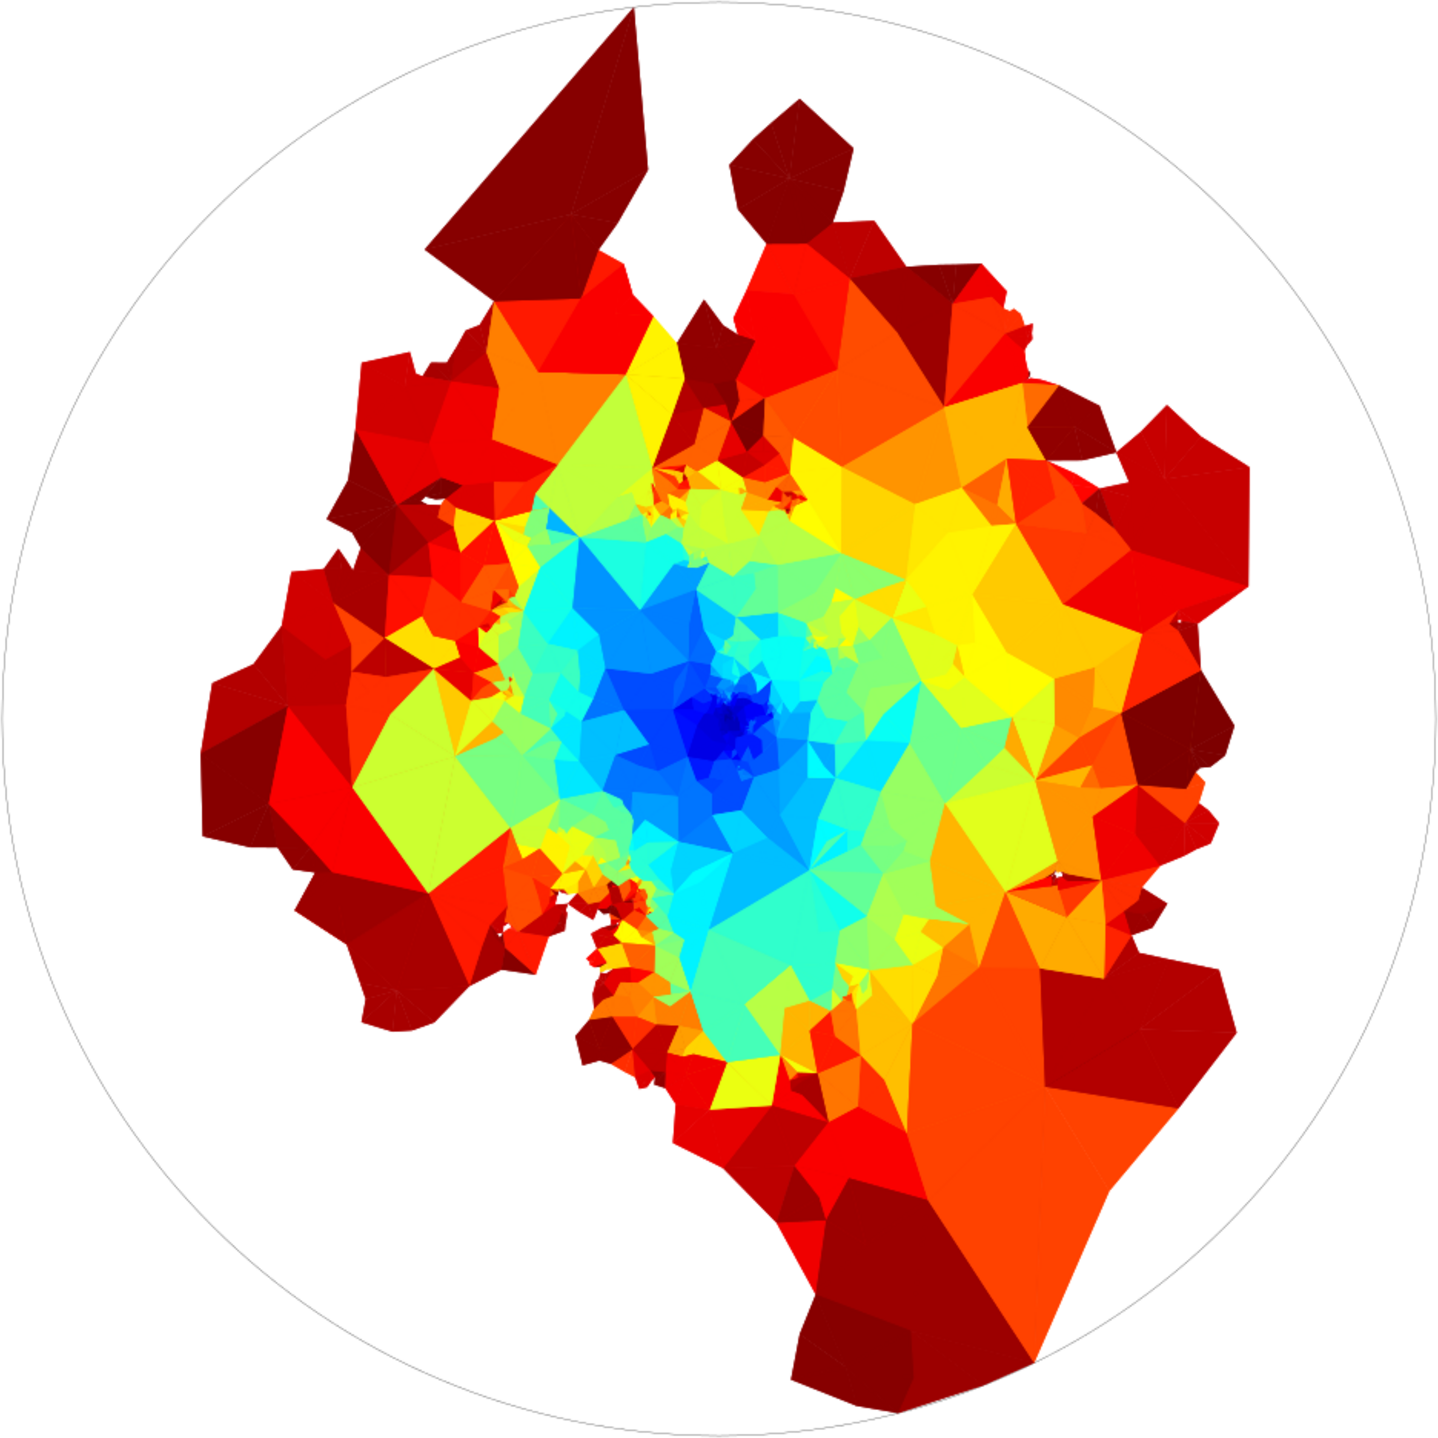
\includegraphics[width=0.35\textwidth]{Figures/mated_crt_10000_8_IDLA.png} 
	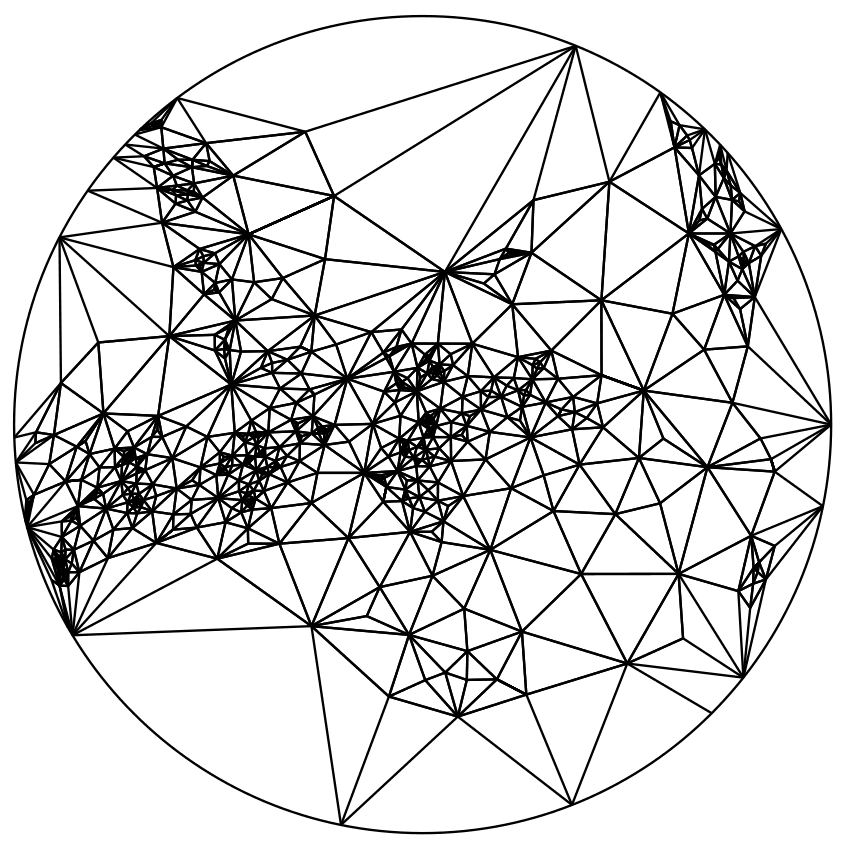
\includegraphics[width=0.35\textwidth]{Figures/mated-crt-1000.png}
	\caption{\textbf{Left:} IDLA on the Tutte embedding of a finite $\gamma = \sqrt{2}$ mated-CRT map with boundary, with $10^4$ vertices. 
		Walkers are added until the first time one of them hits a boundary vertex.  
		Cells are colored according to the first time one of their vertices is hit by a random walk. 
		\textbf{Right:} Illustration of the graph upon which IDLA is run. The finite mated-CRT map with boundary can be constructed from a pair of conditioned Brownian motions via a similar procedure as in Definition~\ref{def:mated-crt-map}. Away from the boundary, it locally looks like the infinite mated-CRT map considered in this paper, but its Tutte embedding is easier to define and simulate. See Remark~\ref{remark:tutte} for further discussion.
	}
	\label{fig:IDLA-tutte-embedding}
\end{figure}
In this article we study the large-scale behavior of a random growth model (IDLA) on a random graph (the mated-CRT map)
which approximates a random fractal surface embedded in the plane (Liouville quantum gravity, LQG). We establish, for each $\gamma \in (0,2)$, the convergence in probability of the IDLA cluster on the $\gamma$-mated-CRT map to a so-called $\gamma$-LQG harmonic ball (Theorem~\ref{theorem:convergence-of-IDLA}). Harmonic balls are random subsets of the plane characterized by a mean-value property for harmonic functions with respect to the LQG measure (Definition~\ref{def:harmonic-ball}). In a companion work \cite{bou2022harmonic}, harmonic balls are constructed via Hele-Shaw flow and it is shown that they are neither Lipschitz domains nor LQG metric balls. 

\subsection{Background}
We now briefly and somewhat informally describe the aforementioned objects, delaying the more technical definitions to Section \ref{sec:preliminaries} below. Minimal prior knowledge of LQG is needed to read this article.


\subsubsection{Internal DLA} \label{subsubsec:idla-informal-intro}
{\it Internal diffusion limited aggregation} (Internal DLA or IDLA) was first introduced to model the physical process of `material removal'
by Meakin-Deutch in \cite{meakin1986formation}. It was also independently introduced by Diaconis-Fulton in  \cite{diaconis1991growth}  as a special case of a commutative algebra.

In its simplest form, IDLA produces an increasing sequence of subsets of the vertex set of a graph $G$ (often taken to be a lattice such as $\Z^2$) as follows. Fix a root vertex $o$ for $G$. Send out an explorer starting from $o$ and allow it to travel according to a simple random walk on $G$ until it reaches an unoccupied vertex, at which point it stops and occupies that vertex. This process is repeated, each explorer starts at the root and walks randomly until it reaches an unoccupied vertex. For $n \geq 1$, the time $n$ IDLA {\it cluster} is the collection of occupied vertices after $n $ iterations of this. 

Following remarkable work by several groups of mathematicians, the large $n$ behavior of the IDLA clusters is now well understood on several families of graphs: $\Z^d$
\cite{lawler1992internal, lawler1995subdiffusive,asselah2013logarithmic, asselah2013sublogarithmic,jerison2012logarithmic, jerison2013internal, jerison2014internal, lucas2014limiting, idla-uniform-starting-points, darrow2020convergence},
Cayley graphs of groups with polynomial \cite{blachere2001internal} and  exponential \cite{blachere2007internal, huss2008internal} growth, supercritical percolation clusters \cite{shellef2010idla, duminil2013containing}, Sierpinski gasket graphs \cite{chen2017internal}, comb lattices \cite{huss-sava-comb, asselah2016fluctuations}, and cylinders \cite{jerison2014chapter, levine2019long, silvestri2020internal}. In most of these cases, the scaling limit of the IDLA clusters is described by a metric ball in the corresponding ambient space (the main result of the paper will give an example where the scaling limit of IDLA is not a metric ball).

We would like to examine what happens when $G$ is taken to be a {\it random} graph embedded in the plane. Specifically, instead of taking some deterministic lattice
which approximates Euclidean space, we take $G$ to be a graph which approximates a {\it Liouville quantum gravity} (LQG) surface.

\subsubsection{Liouville quantum gravity}	
LQG was introduced by Polyakov in the 1980s in the context of bosonic string theory~\cite{polyakov-qg1} as a model of a `random two-dimensional Riemannian manifold'. LQG is too rough to be defined as a manifold in the rigorous sense, although the following loose description can be made precise via various regularization procedures.
For $\gamma \in (0,2)$ and a domain $D\subset\C$, a $\gamma$-LQG surface parameterized by $D$ is the two-dimensional Riemannian manifold with Riemannian metric tensor $e^{\gamma h} \, (dx^2+dy^2)$, where $dx^2+dy^2$ is the Euclidean metric tensor and $h$ is a variant of the Gaussian free field (GFF) on $D$. 

Of particular relevance to this work is the associated volume form, the {\it $\gamma$-Liouville measure} or {\it $\gamma$-LQG measure}. This is a Radon measure
on $D$ which is (informally) given by 
\begin{equation} \label{eq:lqg-measure}
\mu_h(dz) = e^{\gamma h(z)} \, d z, 
\end{equation}
where $dz$ denotes two-dimensional Lebesgue measure~\cite{kahane1985chaos,rhodes-vargas-log-kpz,duplantier2011liouville}. We will give a precise definition of $\mu_h$ and the relevant variants of the GFF in Section \ref{sec:preliminaries}. For now,	the reader only needs to know that $\mu_h$ is a random non-atomic, locally finite Radon measure on $D$ which assigns positive mass to every open subset of $D$ and is mutually singular with respect to Lebesgue measure.
The works~\cite{ding2020tightness,gm-uniqueness} showed that an LQG surface can also be endowed with a canonical random metric, but we will not need this metric in the present paper.



\subsubsection{Random planar maps and the mated-CRT map} \label{subsubsec:mated-crt-map-intro}
\begin{figure}[ht!]\begin{center}
		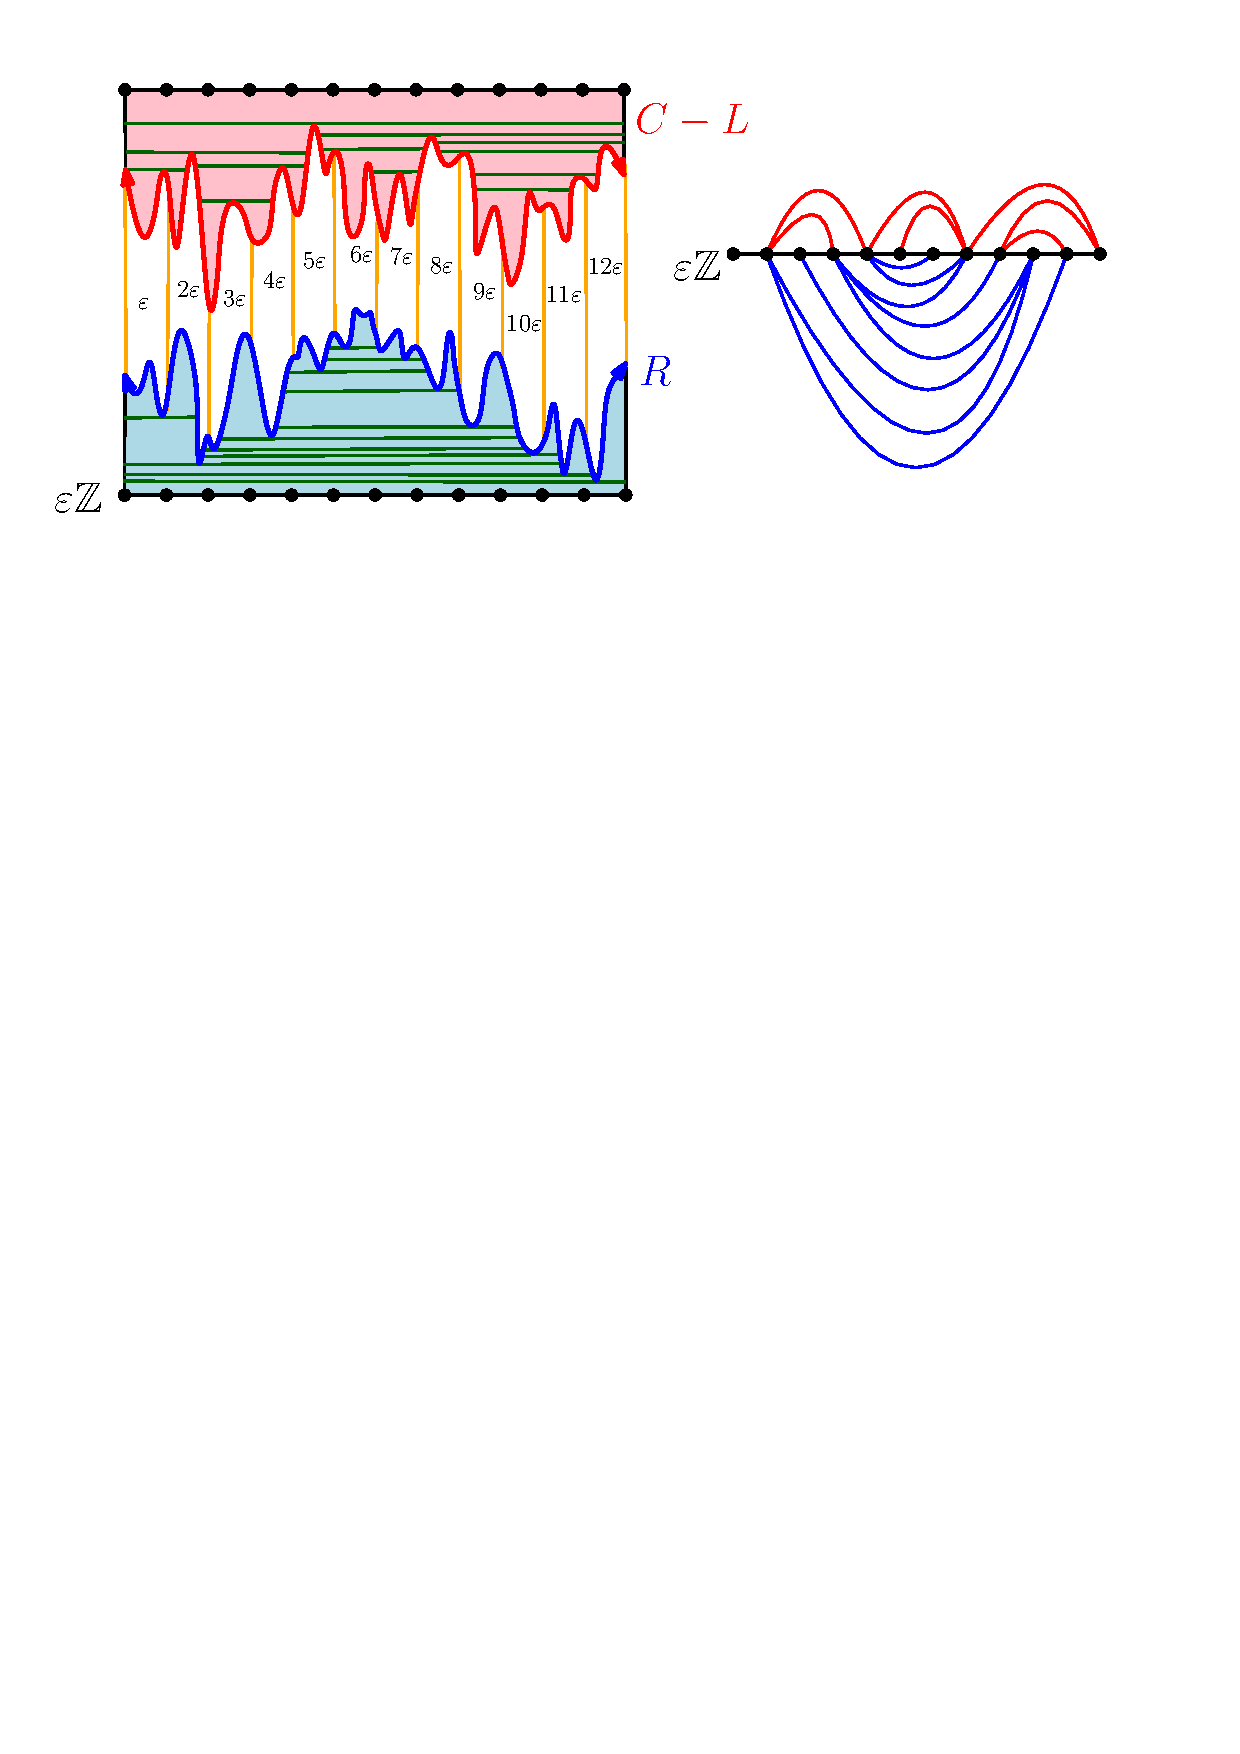
\includegraphics[scale=.8]{Figures/fig-mated-crt-map-harmonic}
		\caption{{\textbf{Left:} A sample construction of the mated-CRT map. We draw the graphs of $C-L$ and $ R$ in the interval $[0, 12 {\eps}]$ 
				where $C$ is a large constant chosen so that the graphs do not intersect. Each vertical strip containing the interval $[a-{\eps}, a]$ for $a \in {\eps} \Z$  corresponds to a vertex
				in the mated-CRT map. The adjacency condition \eqref{eq:edge-map} for $L$ (resp.\ $R$) corresponds to two vertices $a,b \in {\eps} \Z$ being adjacent if there is a horizontal line segment above the graph of $C-L$ (resp.\ below the graph of $ R$) which intersects the graph only in the vertical strips which contain the intervals $[a-{\eps}, a]$ and $[b-{\eps},b]$.
				In the figure, we have illustrated, for each pair $(a,b)$ for which this adjacency condition holds, the lowest (resp.\ highest) such horizontal line segment in green.
				\textbf{Right:} A planar embedding of the mated-CRT map on the left, under which it is a triangulation. Edges arising from the adjacency condition for $L$ (resp.\ $R$) which do not join consecutive vertices are shown in red (resp.\ blue). Edges joining consecutive vertices are shown in black. A similar illustration appeared as~\cite[Figure 1]{gms-harmonic}.}}
		\label{figure:mated-crt-map-illustration}
	\end{center}
\end{figure}


LQG is widely expected, and in some cases rigorously known, to describe the scaling limit of 
{\it random planar maps}. A \textit{planar map} is a graph embedded in $\C$ in such a way that no two edges cross, viewed modulo orientation preserving homeomorphisms $\C \rightarrow \C$. 
Uniform random planar maps (including uniform triangulations, quadrangulations, etc.) converge to $\sqrt{8/3}$-LQG surfaces in the Gromov-Hausdorff sense~\cite{legall-uniqueness,miermont-brownian-map,lqg-tbm1,lqg-tbm2} and, in the case of triangulations, when embedded via the so-called \textit{Cardy embedding}~\cite{hs-cardy-embedding}. Similar convergence results are expected to hold for various types of non-uniform random planar maps toward $\gamma$-LQG with $\gamma\not=\sqrt{8/3}$. For example, random planar maps sampled with probability proportional to the Ising model partition function are expected to converge to $\sqrt 3$-LQG (see, e.g.,~\cite[Section 3.1]{ghs-mating-survey} for more on such conjectures).

Mated-CRT maps are a one-parameter family of random planar maps, indexed by $\gamma\in(0,2)$, whose connection to LQG is better understood than for most other random planar maps. In particular, it was proven by Gwynne-Miller-Sheffield \cite{gms-tutte, gms-random-walk} that the re-scaled counting measure on vertices of the $\gamma$-mated-CRT  map converges to the $\gamma$-LQG measure when the map is embedded into $\C$ via the \emph{Tutte embedding} (i.e., the embedding where the position of each vertex is the average of the positions of its neighbors). Building on this, it was also shown by Berestycki-Gwynne in \cite{berestycki2020random} that random walk on the mated-CRT map converges to so-called \emph{Liouville Brownian motion}, see Section \ref{subsec:lbm-and-rw}
for the definition. 



The mated-CRT map is built via a pair of correlated linear Brownian motions as in Figure \ref{figure:mated-crt-map-illustration}. 
\begin{definition}[Mated-CRT map] \label{def:mated-crt-map}
	Fix $\gamma \in (0,2)$ and consider a two dimensional Brownian motion $(L_t,R_t)_{t\in\R}$ started at the origin with correlation coefficient given by $ - \cos ( \pi \gamma^2/ 4)$.  For ${\eps} > 0$, the {\it $\gamma$-mated-CRT map} with cell size ${\eps}$ associated to $(L_t, R_t)_{t\in\R}$ is the graph ${\Geps}$ whose vertex set is ${\eps} \Z = {\VGeps}$, with two vertices $a < b$ connected by an edge if and only if
	\begin{equation} \label{eq:edge-map}
	\left( \inf_{t \in [a - {\eps},a]} X_t \right) \vee \left( \inf_{t \in [b - {\eps}, b]} X_t \right)\le \inf_{t \in [a, b - {\eps}]} X_t
	\end{equation}
	where $X$ can be either $L$ or $R$. There are two edges connecting $a$ and $b$ if $|b-a| > {\eps}$ and \eqref{eq:edge-map}
	is satisfied for both $L$ and $R$.  See Figure \ref{figure:mated-crt-map-illustration} for an illustration and a description of the planar map structure of $\mathcal {\Geps}$.
\end{definition}

By Brownian scaling, the law of ${\Geps}$ (as a graph) does not depend on ${\eps}$. However, ${\eps}$ is a convenient scaling parameter when talking about limits, as we will see just below.
The definition of the mated-CRT map is a semi-discrete generalization of so-called \emph{mating-of-trees bijections} between random planar maps and random walk excursions.
For instance, the \emph{Mullin bijection}~\cite{mullin-maps,bernardi-maps,shef-burger} is a discrete analog of Definition~\ref{def:mated-crt-map} which produces a planar map decorated by a spanning tree from a two-dimensional random walk excursion.  See~\cite{ghs-mating-survey} for a survey of mating-of-trees bijections and their applications.

The main reason why the mated-CRT map is more tractable than other random planar maps is that, due to the results of~\cite{duplantier2014liouville}, it has an \textit{a priori} embedding into $\C$ defined in terms of LQG and Schramm-Loewner evolution (SLE). We will now discuss this embedding.


\subsubsection{SLE/LQG embedding}
In this paper, we work with an embedding of the mated-CRT map constructed via a space-filling Schramm-Loewner evolution (SLE) curve. We remark, however, that by \cite{gms-tutte, berestycki2020random}, our results extend 
to the so-called Tutte (or harmonic) embedding of the mated-CRT map --- see Figure \ref{fig:IDLA-tutte-embedding} and Remark \ref{remark:tutte}. 

Let $h$ be the random distribution on $\C$ corresponding to a $\gamma$-quantum cone (a slight modification of the whole-plane GFF).
Let $\mu_h$ be the $\gamma$-LQG measure associated to $h$. 
Let $\eta$ be a whole-plane space-filling SLE, independent of $h$, with parameter $\kappa = 16/\gamma^2 \in (4,\infty)$.
We parameterize $\eta$ so that $\eta(0) = 0$ and $\mu_h(\eta([a,b])) = b-a$ for every $a,b\in\R$ with $a < b$. 
We will review the definitions of $h$ and $\eta$ in Section \ref{sec:preliminaries} below.
For now, the unfamiliar reader can just think of $\eta$ as a random continuous, space-filling curve in $\C$ from $\infty$ to $\infty$ parameterized by a locally finite Radon measure. 

\begin{definition}[SLE/LQG embedding of the mated-CRT map~\cite{duplantier2014liouville}] \label{def:sle-lqg-embedding}
	For $\gamma \in (0,2)$ and ${\eps} > 0$, let ${\Geps}$ be the ${\eps}$-mated CRT map with vertex set ${\VGeps}$ as defined in Definition \ref{def:mated-crt-map}.
	The SLE/LQG embedding is defined as follows. Each vertex $a \in {\VGeps} = {\eps}\Z$ corresponds to a \emph{cell},
	\begin{equation} \label{eq:sle-cell}
	\Heps{a} := \eta([a-{\eps}, a]) .
	\end{equation} 
	Two distinct vertices $a,b \in {\VGeps}$ are connected by one (resp. two) edges if and only if $\Heps{a} \cap \Heps{b}$ has one
	(resp. two) connected components which are not singletons.  This provides an embedding
	of ${\Geps}$ into $\C$ by sending each vertex $a \in {\VGeps}$ to the point $\eta(a) \in \Heps{a}$ then drawing edges between adjacent vertices in such a way that no two edges cross (the precise locations of the edges is unimportant for our purposes). 
\end{definition}

The equivalence of the above SLE/LQG description of the mated-CRT map and the Brownian motion description, Definition \ref{def:mated-crt-map}, 
is a consequence of the main result of the seminal work~\cite{duplantier2014liouville}. See, in particular, \cite[Lemma 8.8]{duplantier2014liouville}. For an illustration of the SLE/LQG embedding, see Figure \ref{fig:sle-lqg-embedding}. 

\begin{figure}
	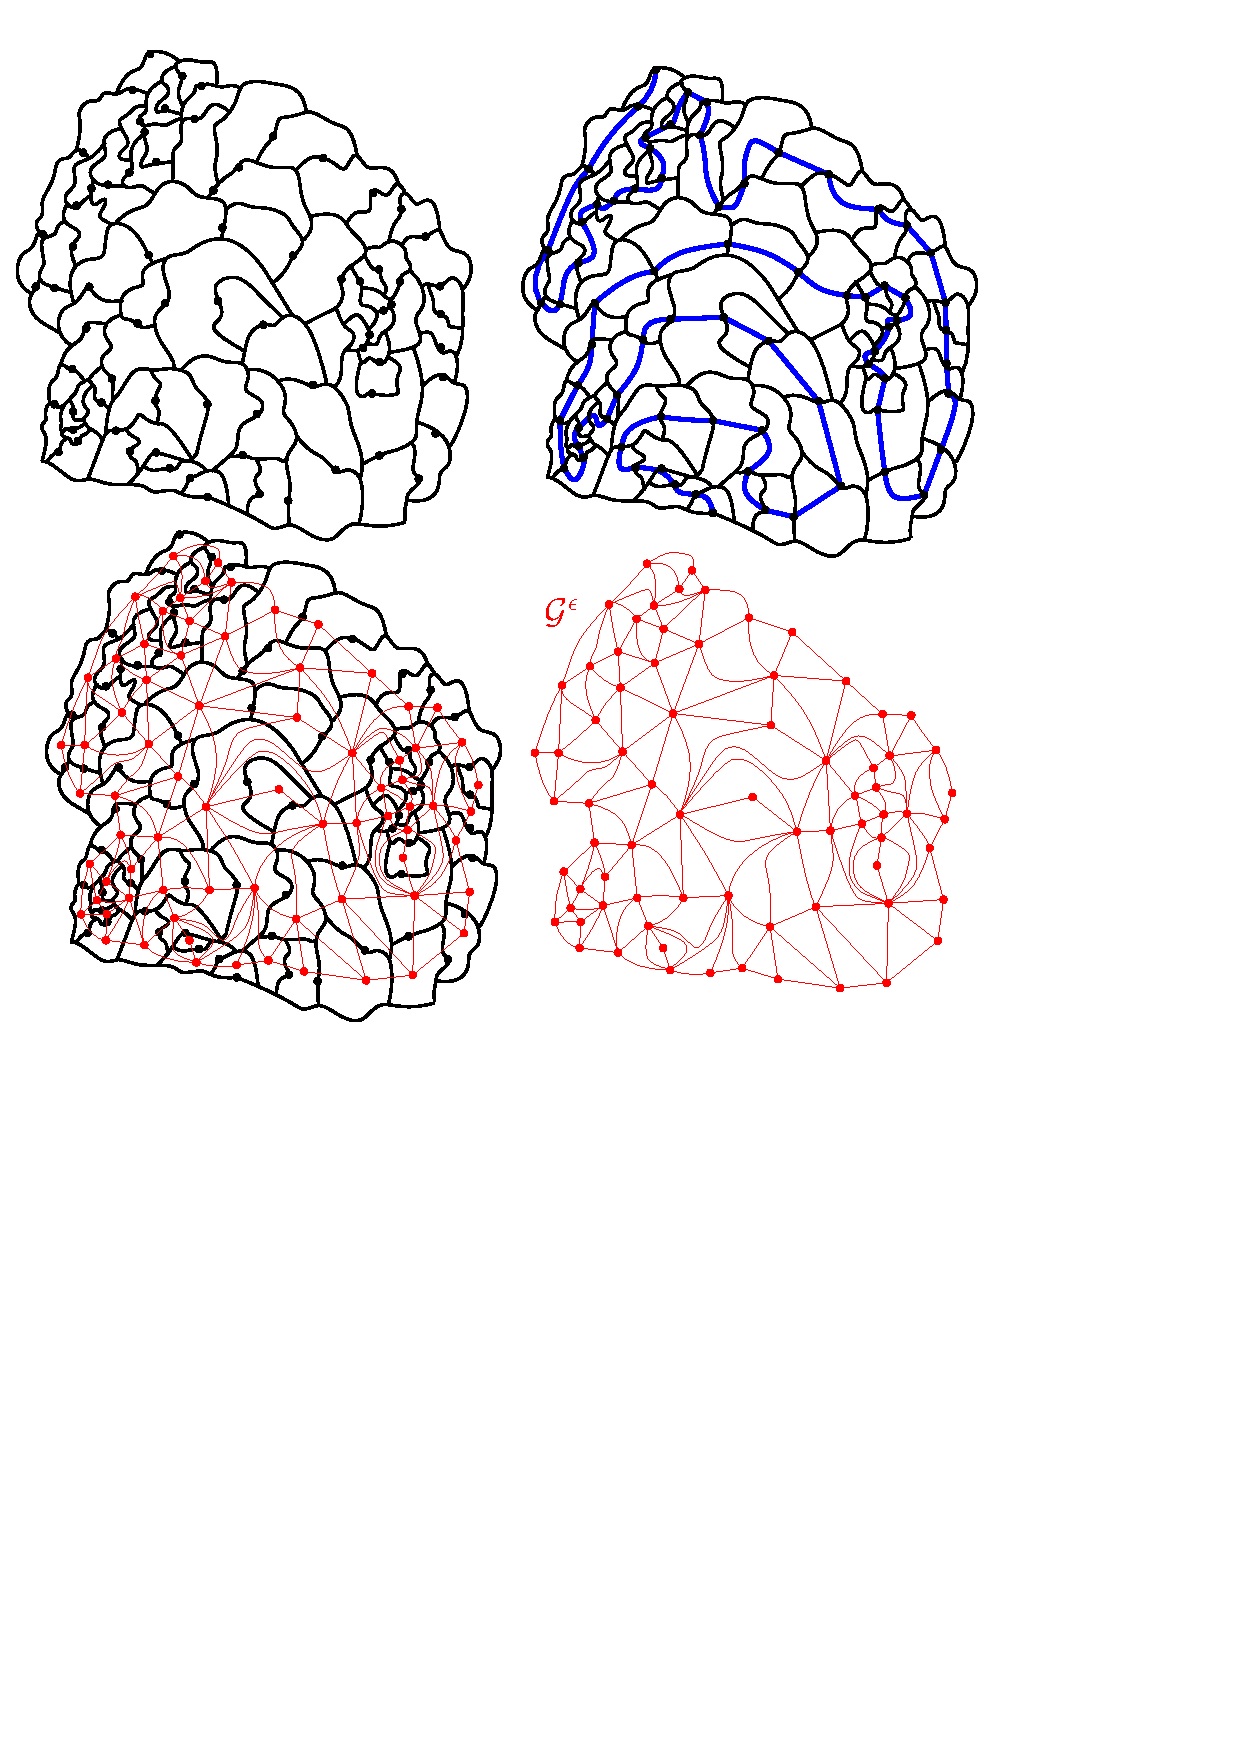
\includegraphics[width=0.75\textwidth]{Figures/fig-structure-graph-def.pdf}
	\caption{\textbf{Top left:} A space-filling SLE curve $\eta$ for $\kappa \geq 8$ divided into cells $\eta([a - {\eps}, a])$ for a collection of $a \in {\eps} \Z$. \textbf{Top right:} The
		same curve with a blue path showing the order in which cells are traversed by $\eta$.	\textbf{Bottom left:} A point in each cell, corresponding to a vertex in ${\Geps}$, is displayed in red
		and red edges are drawn to adjacent neighbors. \textbf{Bottom right:} The same as bottom left but with the black edges removed --- this illustrates the embedding of ${\Geps}$ into $\C$.
		A similar figure has appeared previously as~\cite[Figure 4]{gms-harmonic}.} \label{fig:sle-lqg-embedding}
\end{figure}


\subsubsection{Harmonic balls}	\label{subsubsec:harmonic-ball-intro}
In this article we show that IDLA on the SLE/LQG embedding of the mated-CRT map converges to a {\it harmonic ball}.
\begin{definition}[Harmonic ball] \label{def:harmonic-ball}
	Fix $\gamma \in (0,2)$ and let $\mu_h$ be the LQG measure \eqref{eq:lqg-measure} where $h$ is a variant of the Gaussian free field.
	A $\gamma$-LQG {\it harmonic ball} is a domain $\Lambda \subset \C$ which satisfies the following mean-value property for harmonic functions:
	\begin{equation}
	\int_{\Lambda} f(y) d \mu_h(y) = \mu_h(\Lambda) f(0), \quad \forall \mbox{$f:\C \to \R$ harmonic in a neighborhood of $\cl(\Lambda)$}. 	
	\end{equation}
\end{definition}
In a companion paper \cite{bou2022harmonic}, it is shown that if $\gamma\in(0,2)$ and $h$ is a suitable variant of the GFF on $\C$, then there is a unique growing family of LQG harmonic balls $\{\Lambda_t\}_{t>0}$, parameterized so that $\mu_h(\Lambda_t)=t$. These harmonic balls are constructed directly in the continuum via a certain optimization problem involving the measure $\mu_h$. This optimization problem, as well as several important properties of harmonic balls proved in \cite{bou2022harmonic}, are used in our proof. A statement of the facts about LQG harmonic balls which will be needed later appears in Theorem \ref{theorem:harmonic-balls} below. It is also shown in~\cite{bou2022harmonic} that LQG harmonic balls are neither Lipschitz domains nor LQG metric balls.




\subsection{Main results}
Fix $\gamma \in (0,2)$ and for ${\eps} > 0$ let ${\Geps}$ be the ${\eps}$-mated CRT map as in Definition \ref{def:mated-crt-map},
with vertices ${\VGeps}$ embedded into $\C$ via the SLE/LQG embedding as in Definition \ref{def:sle-lqg-embedding}. 
For a set $X \subset \C$ and $\delta > 0$ we denote the $\delta$-outer and $\delta$-inner neighborhoods of $X$ by 
\begin{equation} \label{eq:outer-inner-neighborhoods}
\begin{aligned}
\Bdeltap(X) &:= \{ x \in \C : \dist(x, X) \leq \delta\} \\
\Bdeltam(X) &:= \{ y \in X : \dist(y, X^c) \geq \delta\} 
\end{aligned}
\end{equation}
where $\dist$ denotes Euclidean distance.

\subsubsection{Internal DLA}
Our notation for the IDLA cluster on ${\Geps}$ is as follows. Begin with $A_{{\eps}}(0) = \emptyset$. For $m\geq 1$, inductively let $A_{{\eps}}(m)$ be the union of $A_{{\eps}}(m-1)$ and the first point at which a simple random walk on ${\Geps}$ started at the origin $ 0 \in {\VGeps} $ 
exits $A_{{\eps}}(m-1)$. By filling in the mated-CRT map cells corresponding to vertices in $A_{\eps}$ (Definition~\ref{def:sle-lqg-embedding}) we may map a subset $A_{{\eps}} \subset {\VGeps}$ to a subset of $\C$ via 
\begin{equation} \label{eq:vertex-scaling}
\overline A_{{\eps}} := \bigcup_{a \in A_{{\eps}}} \Heps{a}.
\end{equation}
\begin{theorem} \label{theorem:convergence-of-IDLA} 
	Let $\{\Lambda_t\}_{t\geq 0}$ be the growing family of $\gamma$-LQG harmonic balls with $\mu_h(\Lambda_t) = t$, as discussed just after Definition \ref{def:harmonic-ball}, with $h$ the field corresponding to the $\gamma$-quantum cone, as in Definition~\ref{def:sle-lqg-embedding}.
	For each $\delta > 0$ and $t > 0$, it holds with probability tending to 1 as ${\eps}\to 0$ that the union of the cells corresponding to the time $\lfloor t{\eps}^{-1}\rfloor$-IDLA cluster approximates $\Lambda_t$ in the following sense:
	\[
	\Bdeltam(\Lambda_t)	\subset \overline A_{{\eps}}(\lfloor t {\eps}^{-1} \rfloor) \subset \Bdeltap(\Lambda_t),
	\]
	where $B_{\delta}^{\pm}$ are as in \eqref{eq:outer-inner-neighborhoods}.
\end{theorem}

\begin{remark}[Convergence under the Tutte embedding] \label{remark:tutte}
	One may  also prove a version of Theorem~\ref{theorem:convergence-of-IDLA} for the disk version of the mated-CRT map under the Tutte embedding, as depicted in Figure~\ref{fig:IDLA-tutte-embedding}.
	The quantum disk is the canonical LQG surface with the topology of the disk~\cite{hrv-disk,duplantier2014liouville}. 
	In~\cite{gms-tutte}, the authors introduce a disk version of the mated-CRT map with a distinguished boundary and define its Tutte embedding (the definition of the Tutte embedding is easier for planar maps with boundary, which is why one wants to consider the disk version of the mated-CRT map). 
	They also show that the Tutte embedding of the disk version of the mated-CRT map is close, in the uniform distance, to its SLE/LQG embedding. 
	Using the fact that the generalized function representing the quantum disk behaves like a GFF away from its boundary, one can extend the results of~\cite{bou2022harmonic} to define a growing family of harmonic balls on the quantum disk started at a uniformly sampled interior point and stopped at the first time when they hit the boundary. 
	Via another absolute continuity argument, one can extend the result of Theorem~\ref{theorem:convergence-of-IDLA} to get that the IDLA clusters on the mated-CRT map with the disk topology, stopped at the first time they hit the boundary, converge to harmonic balls on the quantum disk under the SLE/LQG embedding. 
	We will not provide the details of these absolute continuity arguments in this paper, but see~\cite[Section 7.4]{berestycki2020random} and Theorem \ref{theorem:harmonic-balls} below for similar arguments.
	Using the results of~\cite{gms-tutte}, one gets that IDLA clusters on the disk version of the mated-CRT map also converge to harmonic balls under the Tutte embedding. 
\end{remark}



\subsubsection{Divisible sandpile}\label{subsubsec:div-sandpile-informal-intro}
Our proof of convergence of IDLA proceeds by first establishing an analogous result for an auxiliary particle system which may be thought of as the `expected value' of IDLA. 

The {\it divisible sandpile} is a deterministic diffusion process on a graph $G$,
which, to the best of our knowledge, was first introduced by Zidarov \cite[page 108-118]{zidarov1990inverse}
and (independently) studied by Levine in his thesis \cite{levine-thesis}. Start with masses (real numbers) on vertices of a graph and redistribute the mass according to the following rule. Whenever a vertex has mass $t$ larger than one, it is {\it unstable} and {\it topples} by distributing the excess mass, $(t-1)$, to each of its neighbors equally. This process, called {\it stabilizing}, continues until every vertex has mass less than or equal to one. Although stabilizing may take infinite time, if we have a finite amount of mass on an infinite graph, the end configuration exists and does not depend on the order in which unstable sites are toppled \cite{levine2016divisible}. From another perspective, the divisible sandpile is simply the Jacobi iterative algorithm, \eg, \cite[Chapter 10]{golub-matrix-computations}, for solving the Poisson equation.

In one variant of the model, called the {\it single-source} divisible sandpile, we start with a pile of mass $t > 0$ at a root vertex $o$ in $G$ and stabilize. The final collection of vertices which contain some mass is the {\it cluster}. In each IDLA convergence theorem recalled in Section~\ref{subsubsec:idla-informal-intro}, it has been shown that the limit shape of the single-source divisible sandpile cluster coincides with that of IDLA. This relationship was first observed and established on $\Z^d$ by Levine-Peres in \cite{levine2009strong}. See ~\cite{ruszel-divisible} for a survey relating IDLA and the divisible sandpile. 

In our setting, the IDLA cluster also shares the same limit shape as the divisible sandpile. Denote by $D_{{\eps}}(t)$ the divisible sandpile cluster starting with mass $t > 0$ at the origin in ${\Geps}$. 
\begin{theorem} \label{theorem:convergence-of-div-sandpile}	
	Theorem \ref{theorem:convergence-of-IDLA} holds with the divisible sandpile cluster 
	started with mass $t {\eps}^{-1}$ at the origin,  $\overline D_{{\eps}}(t {\eps}^{-1})$, in place of the IDLA cluster 
	started with $\lfloor t {\eps}^{-1} \rfloor$ explorers at the origin, 
	$\overline A_{{\eps}}(\lfloor t {\eps}^{-1} \rfloor)$. 
\end{theorem}
The divisible sandpile has an explicit description in terms of a discrete optimization problem, which we recall in Section \ref{sec:divisible-sandpile} below. 
In particular, from this optimization problem it is easy to deduce that the divisible sandpile cluster enjoys a certain discrete mean-value property; the clusters are 
{\it discrete harmonic balls} \cite[Equation (5)]{levine2010scaling}. From this, it is no surprise that divisible sandpile clusters converge to continuum harmonic balls.

We would also like to point out that the divisible sandpile appears to be the {\it only} way to find discrete harmonic balls. In fact, this property of the divisible sandpile was used to establish logarithmic fluctuations of IDLA around its limit shape in \cite{jerison2012logarithmic, jerison2013internal, jerison2014internal}.
\subsection{Open problems}
We suggest several directions for further study. The most pressing problem is to extend our convergence result to {\it other} 
random planar maps. This problem is mentioned in the companion work~\cite[Problem 1]{bou2022harmonic}.
\begin{problem} \label{prob:planar-map}
	Show that the scaling limit of IDLA and the divisible sandpile on random planar maps, other than mated-CRT maps, is also described by $\gamma$-LQG harmonic balls.
	For example, on a uniform random planar map establish convergence of IDLA to a $\sqrt{8/3}$-LQG harmonic ball. 
\end{problem}
Our proofs of Theorems~\ref{theorem:convergence-of-IDLA} and~\ref{theorem:convergence-of-div-sandpile} rely heavily on the convergence of random walk on the mated-CRT map to Liouville Brownian motion. This fact has not been established for random planar maps besides the mated-CRT map. We speculate that a solution to Problem~\ref{prob:planar-map} which does not use the convergence of random walk might rely on special symmetries of random planar maps, for example, the peeling process for uniform planar maps \cite{angel-peeling, curien-legall-peeling, curien-peeling-notes}. 

The next two questions concern IDLA on the mated-CRT map. While we have established a qualitative convergence theorem much more quantitative results are known on $\Z^d$. Lawler~\cite{lawler1995subdiffusive} used fine estimates on the Green's function in $\Z^d$ to establish subdiffusive fluctuations of IDLA around its limit shape. Later, Asselah-Gaudillère~\cite{asselah2013logarithmic, asselah2013sublogarithmic} and independently Jerison-Levine-Sheffield~\cite{jerison2012logarithmic, jerison2013internal} established logarithmic fluctuations. We do not expect logarithmic fluctuations in our setting, mainly because the cell sizes in the mated-CRT map have  a `multi-fractal' behavior. See Figure \ref{fig:idla-interface}.
\begin{problem} \label{prob:rate of convergence}
	Provide bounds on the rate of convergence of IDLA on the mated-CRT map. 
\end{problem}
\begin{figure}
	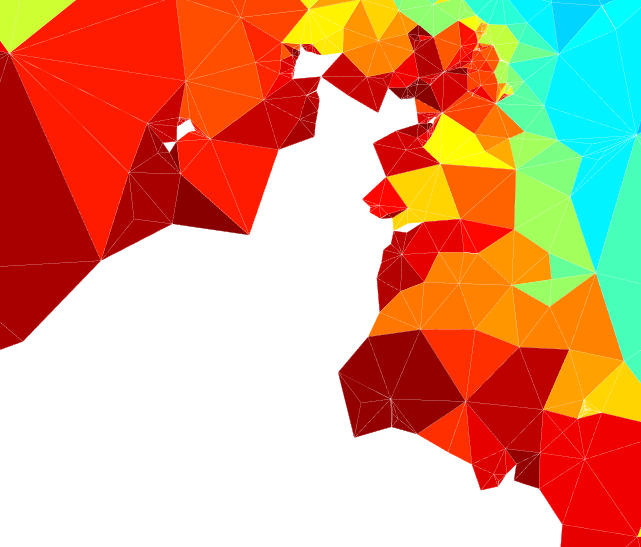
\includegraphics[width=0.45\textwidth]{Figures/mated_crt_10000_8_IDLA_zoom.png}
	\caption{A close up of the interface in Figure \ref{fig:IDLA-tutte-embedding}.} \label{fig:idla-interface}
\end{figure}



After proving logarithmic fluctuations in $\Z^d$, in a remarkable work, Jerison-Levine-Sheffield showed that the scaling limit of the fluctuations themselves exists.
Namely, fluctuations of IDLA on $\Z^d$ converge weakly to a variant of the Gaussian free field \cite{jerison2014internal, jerison2014chapter}. Darrow extended 
the analysis of Jerison-Levine-Sheffield on $\Z^2$ to the case of multiple sources \cite{darrow2020scaling}.
\begin{problem} \label{prob:fluctuations}
	Do the fluctuations of IDLA on the mated-CRT map around its limit shape have a scaling limit? 
\end{problem}


\subsection{Paper and proof outline}
Our proof uses three main inputs; the pairing of IDLA and the divisible sandpile, 
regularity properties of the mated-CRT map, and the convergence of random walk on the mated-CRT map to Liouville Brownian motion. 

The connection between IDLA and the divisible sandpile was implicit in the first work on IDLA by Lawler-Bramson-Griffeath \cite{lawler1992internal}
and made explicit in the thesis of Levine \cite{levine-thesis}. In particular, following the arguments of \cite{lawler1992internal},
a lower bound on the divisible sandpile cluster implies the same lower bound for the IDLA cluster. 
The divisible sandpile, being deterministic and enjoying a variational description, \ie, the {\it least action principle} for its {\it odometer} (see Section \ref{sec:divisible-sandpile} below for definitions), is more tractable than IDLA. 

In the cases considered so far, \eg, \cite{levine2009strong,  huss-sava-comb, MR3957187}, 
convergence of the divisible sandpile is proved by explicitly bounding its odometer via sharp estimates on stopped Green's functions.  These sharp estimates are unavailable in our setting and hence we proceed with a somewhat more robust method. Roughly, we use the fact that the mated-CRT map has an elliptic Harnack inequality and random walk converges to Brownian motion to show that the divisible sandpile odometer converges to its continuum counterpart, the odometer for {\it Hele-Shaw flow} (the solution to the optimization problem used to construct harmonic balls). 

We start by recalling in Section \ref{sec:preliminaries} several mated-CRT map estimates and the invariance principle for random walk 
proved in \cite{berestycki2020random, gwynne2019harmonic}. In this section we also record some basic properties of harmonic balls and Hele-Shaw flow on an LQG surface which we proved in a companion paper \cite{bou2022harmonic}.

In Section \ref{sec:dirichlet-problem}, we use the estimates proved in \cite{berestycki2020random, gwynne2019harmonic} to establish a 
general tightness lemma (Lemma \ref{lemma:discrete-potential-tightness}) for bounded functions with bounded graph Laplacian 
on the mated-CRT map. We then use this lemma to establish the convergence of solutions to the discrete Dirichlet problem on the mated-CRT map to solutions of the continuum Dirichlet problem (Lemma \ref{lemma:discrete-dirichlet-problem}) and convergence of the discrete Green's kernel to the continuum Green's function (Lemma \ref{lemma:uniform-convergence-of-greens-function}). 

In Section \ref{sec:divisible-sandpile}, we define the odometer for the divisible sandpile model on the mated-CRT map and state some basic properties of it which are proved in the Appendix, Section \ref{sec:obstacle-appendix}. 
We then prove convergence of the divisible sandpile odometer to its continuum counterpart. Our proof method is similar to, but easier than, that used to show convergence of the {\it Abelian sandpile odometer} \cite{bourabee-sandpile-2021, pegden-smart-sandpile-2013, barles-souganidis-convergence-1991}.
In Section \ref{sec:divisible-sandpile} we also observe that the convergence of the divisible sandpile odometer implies a lower bound on the divisible sandpile cluster: \ie, for fixed $t , \delta > 0$ it holds with probability tending to 1 as ${\eps}\to 0$ that
\begin{equation} \label{eq:div-lower-outline}
\Bdeltam(\Lambda_t) \subset \overline D_{{\eps}}( t {\eps}^{-1} ).
\end{equation}

In Section \ref{sec:idla-lower-bound} we apply the technique of Lawler-Bramson-Griffeath \cite{lawler1992internal} together with the divisible sandpile lower bound~\eqref{eq:div-lower-outline} and random walk estimates proved in \cite{berestycki2020random} to prove an analogous lower bound for the IDLA cluster.
In fact, the lower bound holds for the {\it stopped} IDLA cluster where random walkers which exit (a mated-CRT map approximation of) $\Lambda_t$ are stopped. 
By the Abelian property of IDLA, Lemma \ref{lemma:abelian-IDLA}, the IDLA cluster can be built by first generating the stopped IDLA cluster and then restarting
the stopped random walkers. 
Thus, an upper bound of the form 
\begin{equation} \label{eq:idla-upper-outline}
\overline A_{{\eps}}(\lfloor t {\eps}^{-1} \rfloor) \subset \Bdeltap(\Lambda_t)
\end{equation} 
will follow if one can show that the restarted random walks cannot travel further than a Euclidean distance of $\delta$ away from $\Lambda_t$. 

In fact, if the limit shape has the correct size, \ie, has volume equal to the total number of walkers, 
and has a measure zero boundary, then by the lower bound and conservation of mass, the number of restarted walkers can be made arbitrarily small.  These two limit shape properties are true for an LQG harmonic ball, as proved in the companion paper \cite{bou2022harmonic}.  Therefore, the proof of the upper bound then reduces to controlling the behavior of order $\delta {\eps}^{-1}$ restarted random walks near the boundary of $\Lambda_t$.  We do this by combining the arguments 
of \cite{duminil2013containing} together with those from LQG theory. 

Specifically, it was shown by Duminil-Copin-Lucas-Yadin-Yehudayoff \cite{duminil2013containing} that if a graph is regular enough, namely is volume doubling, and has a metric which can be controlled by the Euclidean metric, then a small number of walkers cannot spread very far. The mated-CRT map does not enjoy these properties, even approximately, and thus we cannot apply the Duminil-Copin-Lucas-Yadin-Yehudayoff argument directly. Instead, we use methods from LQG theory to provide weak harmonic measure estimates for random walk on the mated-CRT map. A modification of the iterative argument of Duminil-Copin-Lucas-Yadin-Yehudayoff then yields the upper bound.  See the beginning of Section \ref{sec:idla-upper-bound} for a detailed outline of the argument. 

In Section \ref{sec:div-upper-bound} we use the harmonic measure estimates proved in Section \ref{sec:idla-upper-bound} to prove an upper bound on the divisible sandpile cluster. The argument here is a simplified, discrete version of the upper bound for LQG harmonic balls from \cite[Section 6]{bou2022harmonic}. 

All of the aforementioned results were proved conditional on $t$ being small. In Section \ref{sec:proof-of-convergence} we combine the upper and lower bounds together with a scaling argument to remove this constraint on $t$ and complete the proof. 



\subsection{Notation and conventions}
\begin{itemize}
	\item Inequalities/equalities between functions/scalars are interpreted pointwise.
	\item For a set $D \subset \C$, $\partial D$ denotes its topological boundary, $\cl(D) = D \cup \partial D$ its closure, 
	and $\inte(D)$ its interior. 
	\item For a set $A \subset {\VGeps}$, $\partial A$ is the set of vertices in ${\VGeps} \setminus A$ which are joined by an edge to
	a vertex in $A$ and $\cl(A) = A \cup \partial A$ is its closure.  
	The set $\inte(A)$ are the vertices in $A$ which do not share an edge with a vertex in $A^c$. 
	\item For two sets $X, Y \subset \C$, we write $X \Subset Y$ if $\cl(X) \subset Y$. 
	\item $B_r(x)$ denotes the open ball of Euclidean radius $r > 0$ centered at $x \in \C$, when $x$ is omitted, the ball is centered at 0. 
	When $D \subset \C$, we write $B_{r}(D) = \{x \in \C: \dist(x, D) < r\}$.
	\item For $0 < r_1 < r_2$, denote an open annulus centered at $z \in \C$ by
	\begin{equation} \label{eq:annulus}
	\A_{r_1, r_2}(z) = B_{r_2}(z) \setminus \cl(B_{r_1}(z))
	\end{equation}
	and $\A_{r_1, r_2} := \A_{r_1,r_2}(0)$. 
	\item Let $\{E^{r}\}_{z > 0}$ be a one-parameter family of events. 
	We say that $E^r$ occurs with polynomially high probability as $r \to 0$
	if there exists $p>0$ such that $\P[E^r] \geq 1 - O(r^p)$. 
	\item For two sets $X, Y \subset \C$, we define $\dist(X,Y) = \inf_{x \in X, y \in Y} \dist(x,y)$ where $\dist$ denotes the Euclidean distance between two points. 
	\item For a set $D \subset \C$, $C(D)$ denotes the set of continuous functions on  $D$. 
\end{itemize}

\subsection*{Acknowledgments}
We thank an anonymous referee for helpful comments on an earlier version of this article.
A.B. thanks Charlie Smart and Bill Cooperman for useful discussions. 
A.B. was partially supported by NSF grant DMS-2202940 and a Stevanovich fellowship. 
E.G. was partially supported by a Clay research fellowship.


	
	
	\section{Preliminaries} \label{sec:preliminaries}
	In this section we recall several preliminary results on the Gaussian free field, Liouville quantum gravity, space-filling SLE, harmonic balls, random walk on the mated-CRT map, and Liouville Brownian motion. Of note, we record the convergence of random walk on the mated-CRT map to Liouville Brownian motion \cite{berestycki2020random}
and the regularity properties of $\gamma$-LQG harmonic balls established in \cite{bou2022harmonic}. 


\subsection{Gaussian free field}
In this paper, we work with a particular kind of Gaussian free field $h$ which arises naturally from the scaling limit of random planar maps. 
This field corresponds to an LQG surface called a {\it $\gamma$-quantum cone}. For our purposes we just define the field and give its scaling properties
--- a complete definition of the surface is given in \cite{duplantier2014liouville}.  

We start by defining the {\it whole-plane} Gaussian free field (GFF) $h^{\C}$ which is the centered Gaussian random generalized 
function on $\C$ with covariances
\begin{equation} \label{eq:cov-kernel}
\Cov(h^\C(x), h^\C(y)) := \log \frac{\max(|x|,1) \max(|y|,1)}{|x-y|} ,\quad\forall x,y\in\C .
\end{equation} 
The GFF $h^{\C}$ is not defined pointwise as the covariance kernel in~\eqref{eq:cov-kernel} diverges to $\infty$ as $x\to y$. 
However, for $z\in\C$ and $r>0$, one can define the average of $h^{\C}$ over the circle of radius $r$ centered at $z$, which we denote by $h^{\C}_r(z)$~\cite[Section 3.1]{duplantier2011liouville}. 	The whole plane GFF is sometimes defined modulo additive constant. Our choice of covariance in~\eqref{eq:cov-kernel} corresponds to fixing this additive constant so that $h^\C_1(0) = 0$ (see, e.g.,~\cite[Section 2.1.1]{vargas2017lecture}). 

The circle average of $h^{\C}$, $t \to h^{\C}_{e^{-t}}(0)$ is a Brownian motion, \cite[Section 3.1]{duplantier2011liouville}.
The field corresponding to the $\gamma$-quantum cone is constructed by enforcing its circle-average to correspond to a particular conditioned Brownian motion. 
Fix $\gamma \in (0,2)$ and let 
\begin{equation} \label{eq:Q}
Q := \frac{2}{\gamma} + \frac{\gamma}{2}.
\end{equation}

\begin{definition}[Circle average embedding of the $\gamma$-quantum cone] \label{def:quantum-cone}
	The circle average embedding of the $\gamma$-quantum cone is the distribution $h$ defined as follows. 
	Let $B$ be a standard linear Brownian motion and let $\hat{B}$ be an independent standard linear Brownian motion conditioned so that $\hat{B}_t + (Q-\gamma) t > 0$ for all $t > 0$.
	Let
	\begin{equation}
	A_t := \begin{cases}
	B_t + \gamma t , \quad &t \geq 0 \\
	\hat{B}_{-t} + \gamma t ,\quad &t < 0 .
	\end{cases}
	\end{equation}  
	The distribution $h$ is defined so that $t \to h_{e^{-t}}(0)$ has the same law as the process $A$ and $h - h_{|\cdot|}$ is independent 
	from $h_{|\cdot|}$ and has the same law as the analogous process for the whole-plane GFF, $h^{\C}$. 
\end{definition}


We note that the field $h$ in Definition \ref{def:quantum-cone} has the property that $\sup \{ r > 0 : h_r(0) + Q \log r = 0 \} = 1$. Furthermore, it is immediate from Definition~\ref{def:quantum-cone} that $h$ restricted to the unit disk agrees in law with the corresponding restriction of a whole-plane GFF plus $ - \gamma \log |\cdot|$, normalized so that its circle average over the disk is zero:
\begin{equation} \label{eq:gff}
h|_{B_1} \overset{d}{=} ( h^{\C} - \gamma \log |\cdot| )|_{B_1} .
\end{equation}


The law of the whole-plane GFF, viewed modulo additive constant, is invariant under complex affine transformations of $\C$. This implies the following scaling property for $h^{\C}$,
\begin{equation} \label{eq:gff-scaling}
h^{\C} \overset{d}{=} h^{\C}(x\cdot +y) - h^{\C}_{|x|}(y), \quad \forall x \in \C \setminus \{0\}, \quad \forall  y \in \C. 
\end{equation}
The distribution $h$ has a similar scale invariance. For $b > 0$, let 
\begin{equation} \label{eq:cone-scale-radius}
R_b := \sup \{ r > 0 : h_r(0) + Q \log r = \frac{1}{\gamma} \log b\}.
\end{equation}
Then, by \cite[Proposition 4.13(i)]{duplantier2014liouville},
\begin{equation} \label{eq:quantum-cone-scaling}
h(R_b \cdot) + Q \log R_b - \frac{1}{\gamma} \log b \overset{d}{=} h. 
\end{equation}	


\subsection{Liouville quantum gravity} \label{subsec:lqg}
\textit{Liouville quantum gravity (LQG)} is a one-parameter family of random fractal surfaces which were introduced by Polyakov in the 1980s in the context of bosonic string theory~\cite{polyakov-qg1}. 
We give some basic properties of LQG and refer the interested reader to the introductory texts \cite{berestycki2021gaussian,sheffield-icm,gwynne2020random}.

Let $\mu_h$ denote the {\it $\gamma$-LQG area (Liouville) measure} associated to $h$, the $\gamma$-quantum cone defined in \eqref{def:quantum-cone}. One of the several ways of defining $\mu_h$ is as the a.s.\ weak limit 
\begin{equation} \label{eq:measure-lim}
\mu_h = \lim_{\epsilon \rightarrow 0} \epsilon^{\gamma^2/2} e^{\gamma h_\epsilon(z)} \,dz
\end{equation}
where $dz$ denotes Lebesgue measure and $h_\epsilon(z)$ is the circle average~\cite{duplantier2011liouville, sheffield2016field}.
In fact, the measure $\mu_{\tilde h}$ can be constructed for any random generalized function $\tilde h$ of the form  $h + f$ where $f$ is a possibly random continuous function
and $h$ is the whole-plane GFF, defined in \eqref{eq:gff-scaling}. In particular, this includes the $\gamma$-quantum cone from Definition~\ref{def:quantum-cone}.
For later use, we record some basic properties of the LQG measure. 
\begin{fact}[LQG measure] \label{fact:lqg-measure}
	The LQG area measure $\mu_h$ satisfies the following properties.
	\begin{enumerate}[label=\Roman*.]
		\item {\bf Radon measure.} A.s., $\mu_h$ is a non-atomic Radon measure.
		\item {\bf Locality.} For every deterministic open set $U \subset \C$,
		$\mu_h(U)$ is given by a measurable function of 
		$h \vert_{U}$.
		\item {\bf Weyl scaling.} A.s., $e^{\gamma f} \cdot \mu_h = \mu_{h + f}$
		for every continuous function $f: \C \to \R$. 
		\item {\bf Conformal covariance.} A.s., the following is true. Let $U , \tilde U \subset \C$ be open and let $\phi$ be a conformal
		map from $\tilde U$ to $U$. Then, with $Q$ as in~\eqref{eq:Q}, 
		\begin{equation} \label{eq:measure-coord}
		\mu_{h \circ \phi + Q \log |\phi'|}(A) = \mu_h(\phi(A)) \quad \mbox{for all Borel measurable $A \subset \tilde U$}.
		\end{equation}
	\end{enumerate}
\end{fact}


The first three properties in Fact~\ref{fact:lqg-measure} are immediate from the definition~\eqref{eq:measure-lim}. The conformal covariance property was proven to hold a.s.\ for a fixed conformal map in~\cite[Proposition 2.1]{duplantier2011liouville} and extended to all conformal maps simultaneously in~\cite{sheffield2016field}.




\subsection{Harmonic balls}
A harmonic ball is a domain which satisfies the mean-value property for harmonic functions with respect to the LQG measure --- Definition \ref{def:harmonic-ball}. 
These balls are constructed in a companion work via the following optimization problem. 
For each $t > 0$ and ball $B_r = B_r(0)$, let 
\begin{equation} \label{eq:least-super-solution}
\overline w_t^{B_r} = \inf\{ w \in C(\cl(B_r)) : \Delta w \leq \mu_h \mbox{ in $B_r$}  \mbox{ and }  w \geq  - t G_{B_r}(0, \cdot) \mbox{ in $\cl(B_r)$}\},
\end{equation}
% CORRECTION [C1]: normalisation of $G_{B_r}$ stated (printed: 'Green's function for standard Brownian motion'), consistent with the definition of $\kappa_0$.
where $C(\cl(B_r))$ denotes the set of continuous functions on the closed ball, $\Delta w$ is interpreted in the distributional sense, $G_{B_r}$ is the Green's function on $B_r$ with zero boundary conditions, normalized by $\Delta G_{B_r} = -\delta$ (so that the occupation density of standard Brownian motion killed upon exiting $B_r$ is $2G_{B_r}$), and the infimum is pointwise.
The definition in \eqref{eq:least-super-solution} is the {\it obstacle problem} formulation of Hele-Shaw flow~\cite{sakai1984solutions} and may be thought of as the continuum 
analogue of the odometer for the divisible sandpile, defined below in Section \ref{sec:divisible-sandpile}. 


\begin{theorem}[Combination of Theorems 1.1 and 5.5 and Lemma 3.2 in \cite{bou2022harmonic}] \label{theorem:harmonic-balls}
	On an event of probability one, there exists a unique family of harmonic balls $\{\Lambda_t\}_{t > 0}$
	satisfying the following properties:
	\begin{enumerate}[label=(\alph*)]
		\item For each $t > 0$, $\mu_h(\Lambda_t) = t$, $\mu_h(\partial \Lambda_t) = 0$, and $\Lambda_t$ is equal to the interior of its closure.
		\item The domains $\Lambda_t$ are bounded, connected, open, contain the origin, increase continuously in $t$ (in the Hausdorff topology), and satisfy $\cap_{t > 0} \Lambda_t = \{0\}$.
		\item If, for some $r > 0$, $\Lambda_t \subset B_r$, then, for all $\rho > r$, 
		\[
		\Lambda_t = \inte \left( \cl \left( \{ x \in B_\rho : \overline w_t^{B_\rho}(x) > - t G_{B_\rho}(0, x)\} \right) \right).
		\] 
		Moreover, $\overline w_t^{B_\rho}$ is continuous and
		satisfies
		\[
		\begin{cases}
		\Delta \overline w_t^{B_\rho} = \mu_h |_{\Lambda_t}  \quad \mbox{on $B_\rho$} \\
		\overline w_t^{B_\rho} = 0 \quad \mbox{on $\partial B_\rho$}.
		\end{cases}
		\]
	\end{enumerate}
	
\end{theorem}

Strictly speaking, \cite{bou2022harmonic} considers the case where $h$ is not the quantum cone but rather a whole-plane GFF plus a log-singularity.
Transferring the proof to the quantum cone is a standard absolute continuity argument which we now provide. 
\begin{lemma} \label{lemma:existence-up-to-fixed-time}
	On an event of probability one, there exists a unique family of harmonic balls $\{\Lambda_t\}_{0 < t < T}$
	which satisfies the properties of Theorem \ref{theorem:harmonic-balls} (with $t$ restricted to be in $(0,T)$), where 
	\[
	T = \sup \{ t > 0 : \Lambda_t \subset B_{1/2}\}.
	\]
\end{lemma}
\begin{proof}
	By \eqref{eq:gff}, the restrictions to the unit disk of the quantum cone field $h$ and the whole-plane GFF plus $-\gamma \log |\cdot|$ agree in law.
	Since harmonic balls depend locally on the field~\cite[Proposition 1.3]{bou2022harmonic}, this equality in law together with  \cite[Theorems 1.1 and 5.5 and Lemma 3.2]{bou2022harmonic} directly implies the existence of a family of harmonic balls $\{ \Lambda_t \}_{0 < t < T}$ satisfying the properties in Theorem \ref{theorem:harmonic-balls}. 	
	Uniqueness of such a family is guaranteed by \cite[Proposition 5.6]{bou2022harmonic} 
	(that proposition is stated for a family of harmonic balls defined for all times, but the proof still works if the harmonic balls are only defined up to some fixed time). 
\end{proof}
We will now extend the above construction to all time using the scale invariance property of the $\gamma$-quantum cone.
The following is the quantum cone analog of \cite[Lemma 5.7]{bou2022harmonic} (which gives a similar statement for the LQG harmonic balls associated with the whole-plane GFF).  
\begin{lemma} \label{lemma:scale-invariance-up-to-fixed-time}
	For $b >0$, define the random radius $R_b > 0$ as in~\eqref{eq:cone-scale-radius}.
	A.s., there exists a unique family of harmonic balls 
	$\{\Lambda_{t}\}_{0 < t < b T^b}$
	such that $\{R_b^{-1} \Lambda_{b t}\}_{0 < t < T^b}$
	has the same law as $\{\Lambda_t\}_{0 < t < T}$, 
	where
	$T$ is as in Lemma \ref{lemma:existence-up-to-fixed-time}, 
	and 
	\[
	T^b = \sup\{ t > 0 : R_b^{-1} \Lambda_{b t} \subset B_{1/2} \}.
	\]
	In fact, we have the equality of joint laws
	\[
	\left( h, \{\Lambda_t\}_{0 < t < T} \right) \overset{d}{=}\left( h(R_b \cdot) + Q \log R_b - \frac{1}{\gamma} \log b, \{R_b^{-1} \Lambda_{b t}\}_{0 < t < T^b} \right).
	\] 
\end{lemma}
\begin{proof}
	Fix $b > 0$ and let
	\[
	h^b := h(R_b \cdot) + Q \log R_b - \frac{1}{\gamma} \log b,
	\]
	so that, as in \eqref{eq:quantum-cone-scaling}, $h^b \overset{d}{=} h$. By Lemma \ref{lemma:existence-up-to-fixed-time}, a.s.\ there exists a unique family of harmonic balls $\{\Lambda^b_t\}_{0 < t < T^b}$ which satisfies the properties of Theorem \ref{theorem:harmonic-balls} for the measure $\mu_{h^b}$ (with $t$ restricted to be in $(0,T^b)$), where
	\[
	T^b = \sup\{ t > 0 : \Lambda^b_{t} \subset B_{1/2} \}.
	\]
	Define
	\[
	\Lambda_{b t}  :=   R_b  \Lambda^b_t, \quad \forall 0 < t < T^b
	\]
	and note that by the properties of $\Lambda^b_t$, the LQG coordinate change formula, and Weyl scaling (Fact \ref{fact:lqg-measure}), a.s.,
	\[
	t = \mu_{h^b}(\Lambda^b_t) = b^{-1} \mu_h(\Lambda_{ b t}), \quad \forall 0 < t < T^b.
	\]
	For similar reasons, the domains $\{\Lambda_{t}\}_{0 < t < b T^b}$ are a.s.\ harmonic balls and satisfy parts (a) and (b) of Theorem \ref{theorem:harmonic-balls} for the measure $\mu_h$
	(with $t$ constrained to be less than $b T^b$). 
	These properties are enough to apply \cite[Proposition 5.6]{bou2022harmonic} (which works if the harmonic balls are only defined up to some fixed time) and conclude that $\{\Lambda_{t}\}_{0 < t < b T^b}$ is the unique such family. As $h^{b}$ has the same law as $h$, this shows the equality of joint laws. 
\end{proof}

\begin{proof}[Proof of Theorem \ref{theorem:harmonic-balls}]
	
	
	By Lemma \ref{lemma:scale-invariance-up-to-fixed-time}, a.s.\ for every integer $b \geq 0$, 
	there exists a unique family of harmonic balls $\{\Lambda_{t}\}_{0 < t < b T^b}$
	which satisfies the conditions of the theorem statement up to time $b T^b$,
	where $T^b$ is as in Lemma \ref{lemma:scale-invariance-up-to-fixed-time}. Since $T^b \overset{d}{=} T$ for each $b>0$, where $T$ is as in Lemma \ref{lemma:existence-up-to-fixed-time}, and $T$ is a strictly positive random variable, we deduce that $\lim_{b \to \infty} b T^b = \infty$ in probability. This complete the proof. 
\end{proof}

By applying the proof of Lemma \ref{lemma:scale-invariance-up-to-fixed-time} to the infinite family of harmonic balls given by Theorem \ref{theorem:harmonic-balls}, we have the following.
\begin{lemma} \label{lemma:scale-invariance}
	For each $b > 0$, we have the equality of the joint laws
	\[
	\left( h, \{\Lambda_t\}_{t > 0} \right) \overset{d}{=}\left( h(R_b \cdot) + Q \log R_b - \frac{1}{\gamma} \log b, \{R_b^{-1} \Lambda_{b t}\}_{t > 0} \right).
	\] 
	where the random radius $R_b > 0$ is as in~\eqref{eq:cone-scale-radius}. 
\end{lemma}


\subsection{Whole plane space-filling SLE}
The Schramm-Loewner evolution ($\text{SLE}_{\kappa}$) for $\kappa > 0$ was introduced by Schramm in \cite{schramm-sle}
as the only conformally invariant family of random curves which satisfy the domain Markov property. There are three phases of  $\text{SLE}_{\kappa}$: the curves are simple when $\kappa \in (0,4]$,  have self-intersections but are not space-filling for $\kappa \in (4,8)$, and are space-filling when $\kappa \geq 8$. 

In the embedding of the mated-CRT map, we work with the {\it whole plane space-filling SLE} $\eta$, a variant of SLE introduced in 
\cite[Sections 1.2.3 and 4.3]{miller2017imaginary}.  This is a random space-filling curve $\eta$ in $\C$ 
from $\infty$ to $\infty$ which fills all of $\C$ and does not intersect the interior of its past. 

For context, we informally describe how one constructs space-filling SLE. When $\kappa \geq 8$, whole plane space-filling SLE is simply ordinary SLE. In this case the 
cells $\eta([x- {\eps}, x])$ are topological rectangles and their boundaries are the union of four $\text{SLE}_{\underline{\kappa}}$ curves for $\underline{\kappa} = 16/\kappa$.
When $\kappa \in (4,8)$,  $\eta$ is built by taking ordinary $\text{SLE}_{\kappa}$ and `filling in' bubbles which are disconnected from infinity.
This results in a somewhat complicated geometry. In particular, for $\kappa \in (4,8)$ it is possible for the intersection of two cells to be an uncountable, totally disconnected Cantor-like set. Pairs of cells which intersect in this manner do not correspond to edges of the mated-CRT map in Definition~\ref{def:sle-lqg-embedding}.

In this paper, we mainly just use the fact that the law of $\eta$ is scale-invariant:
\begin{equation} \label{eq:eta-scale-invariant}
r \eta \overset{d}{=} \eta, \quad \forall r > 0, \quad \mbox{when viewed as curves modulo time parameterization}.
\end{equation}
For a detailed treatment of SLE see \cite{werner-notes, lawler-book} and for a more in-depth exposition of whole plane space-filling SLE see \cite[Section 3.6]{ghs-mating-survey}.

\subsection{Mated-CRT map} \label{subsec:mated-crt-prelims}
We defined most of what we need concerning the mated-CRT map in Section \ref{subsubsec:mated-crt-map-intro}. We provide some additional notation which we will use in the sequel. 

We fix the convention that when referring to points in $\C$, we use the letters $x,y,z$; while vertices in the mated-CRT map correspond to letters $a,b$.
Sets in $\C$ are $X, Y, D$, while sets of vertices in the mated-CRT map are $A,B$. 

For ${\eps} > 0$ and $\gamma \in (0,2)$ let ${\Geps}$ be the mated-CRT map with vertex set ${\VGeps}$ embedded in the plane via a whole plane space-filling SLE curve $\eta$ with $\kappa = 16/\gamma^2$  
as in Definitions \ref{def:mated-crt-map} and \ref{def:sle-lqg-embedding}. 

It is important to note that while a.s.\ each vertex in the mated-CRT map has a finite number of neighbors, the number of neighbors may be arbitrarily large. 
Write $\deg^{{\eps}}(a)$ for the degree of $a \in {\VGeps}$. 	We will need a way to pass between vertices in the map and points in $\C$:  for $x \in \C$, let
\begin{equation} \label{eq:plane-to-embedding}
a_x^{{\eps}} := \mbox{(smallest $a \in {\eps} \Z$ such that $x \in \Heps{a}$)}.
\end{equation}
For a set $D \subset \C$, we define 
\begin{equation} \label{eq:cells-domain-restriction}
{\Geps}(D) := \mbox{(subgraph of ${\Geps}$ induced by $\{a \in {\eps} \Z: \Heps{a} \cap D \neq \emptyset\}$)}
\end{equation}
and write ${\VGeps}(D)$ for the vertices in ${\Geps}(D)$. 
Several times throughout the paper we will work with the sets ${\VGeps}(D) \setminus {\VGeps}(\partial D)$ rather than ${\VGeps}(D)$ to account 
for the coarseness of the cells in the mated-CRT map. Indeed, even if $D$ is a smooth, bounded open set, typically ${\VGeps}(D)$ overlaps with ${\VGeps}(\partial D)$ --- see Figure \ref{fig:cell-boundary-mated-crt}.	
\begin{figure}
	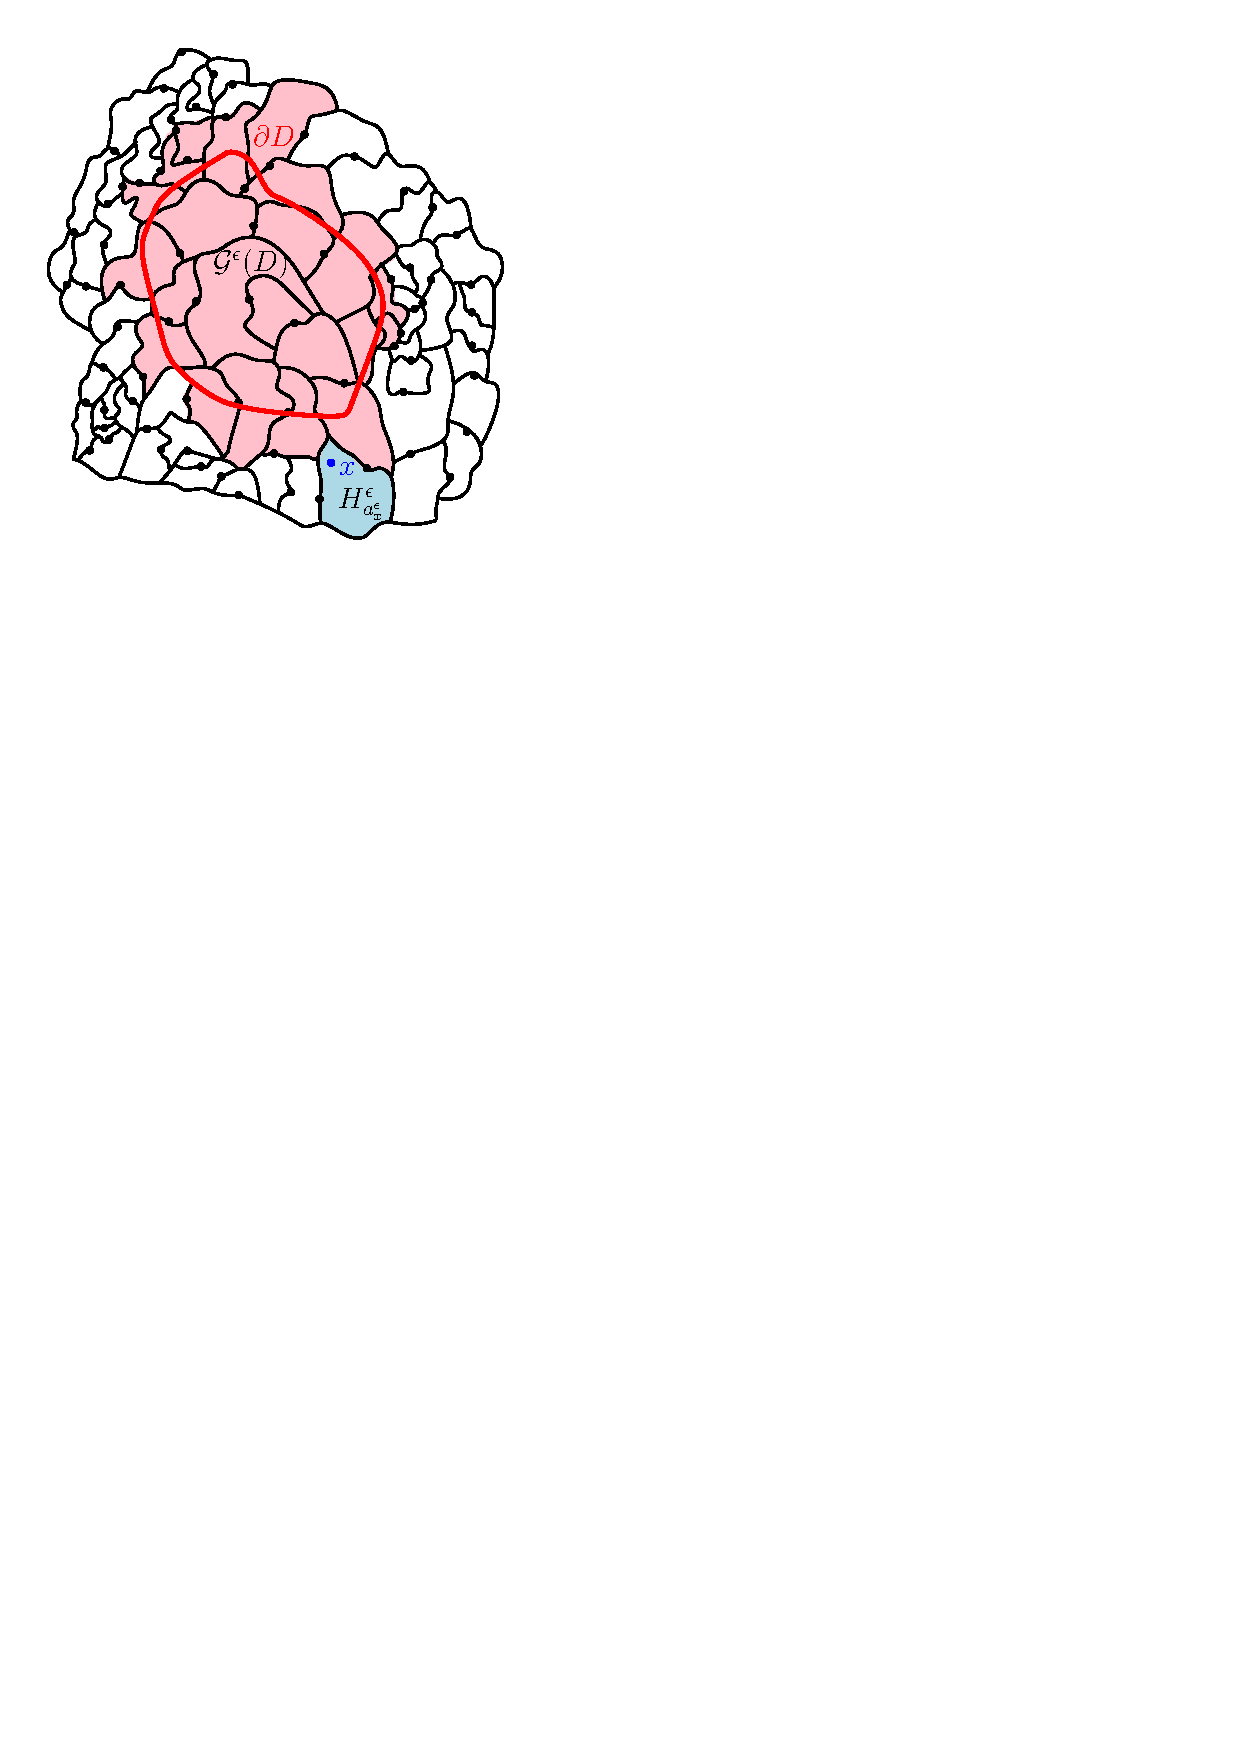
\includegraphics{Figures/fig-structure-graph-restrict.pdf}
	\caption{A set $D\subset \C$ and the set of mated-CRT map cells corresponding to the vertices in ${\Geps}(D)$, as in \eqref{eq:cells-domain-restriction}. 
		The boundary of the domain $\partial D$ is drawn in red and the cells of ${\Geps}(D)$ are filled in pink. A point $x \in \C$ and the cell containing it, $\Heps{a^{{\eps}}_x}$, is drawn 
		in light blue. A similar figure appeared in ~\cite[Figure 5]{gms-harmonic}.} \label{fig:cell-boundary-mated-crt}
\end{figure}



\subsection{Cell size and volume estimates}
In this section, we recall some estimates proved in the appendix of \cite{berestycki2020random}. 
The following estimate gives worst-case upper and lower bounds for the LQG mass of Euclidean balls.  
\begin{lemma}[Lemma A.1 in \cite{berestycki2020random}] \label{lemma:volume-growth}
	For each $\beta^+ \in (0, (2 -\gamma)^2/2)$ and $\beta^- > (2+\gamma)^2/2$
	it holds with polynomially high probability as $\delta \to 0$ that  
	\begin{equation} \label{eq:ball-volume}
	\delta^{\beta^-} \leq \mu_h(B_\delta(z)) \leq \delta^{\beta^+} ,\quad\forall z \in B_{1-\delta} .
	\end{equation}
\end{lemma}
For convenience, we fix $\beta^{\pm}$ in a fashion depending only on $\gamma$ so that when we refer to Lemma 
\ref{lemma:volume-growth} we may just refer to a single choice of $\beta^{\pm}$. 

The next lemma gives similar worst-case upper and lower bounds for the size of the cells in the mated-CRT map. 
\begin{lemma}[Lemma 2.4 in \cite{berestycki2020random}] \label{lemma:cell-size-estimate}
	Fix a small parameter $\zeta \in (0,1)$ and $\rho \in (0,1)$. With polynomially high probability as ${\eps} \to 0$, the Euclidean diameter of each mated-CRT map cell $\Heps{a}$ which intersects $B_\rho$ satisfies 
	\begin{equation}
	{\eps}^{\frac{2}{(2 - \gamma)^2} + \zeta} \leq \mathrm{diam}(\Heps{a}) \leq {\eps}^{\frac{2}{(2 + \gamma)^2} - \zeta}.
	\end{equation}
	
\end{lemma}


The following lemma is a quantitative version of the important fact that the counting measure on vertices in the mated-CRT map converges weakly to the LQG area measure.

\begin{lemma}[Lemma A.4 in \cite{berestycki2020random}] \label{lemma:mu_h-convergence}
	Fix $\rho \in (0,1)$. There exists $\alpha = \alpha(\gamma) > 0$ and $\beta = \beta(\gamma) > 0$
	such that with polynomially high probability as ${\eps} \to 0$, the following is true. 
	Let $D \subset B_{\rho}$ and let $f: B_{{\eps}^{\alpha}}(D) \to [0,\infty)$
	be a non-negative function which is ${\eps}^{-\beta}$-Lipschitz continuous and satisfies $\|f\|_{\infty} \leq {\eps}^{-\beta}$.
	For $a \in {\VGeps}(D)$, let $w^{{\eps}}_a$ be an arbitrary point of $\Heps{a} \cap \cl(D)$. 
	If we let $\mu_h$ be the $\gamma$-LQG area measure induced by $h$, then 
	\begin{equation}
	{\eps}^{-1} \int_D f(z)d \mu_h(z) - {\eps}^{-1 + \alpha} \leq
	\sum_{a \in {\VGeps}(D)} f(w^{\eps}_a) \leq 
	{\eps}^{-1} \int_{B_{{\eps}^\alpha}(D)} f(z) d \mu_h(z)  + {\eps}^{-1 + \alpha}
	\end{equation}
	simultaneously for every choice of $D$ and $f$ as above. 
\end{lemma}


An analogous result to the above holds when cells are weighted by their degrees, in which case, since the mated-CRT map is a planar triangulation,
there is an extra factor of 6 in the limit. 
\begin{lemma}[Corollary A.6 in \cite{berestycki2020random}] \label{lemma:mu_h_degree-convergence}
	For ${\eps}> 0$, let $\mu_h^{{\eps}}$ be the measure whose restriction to each cell $\Heps{a}$ for $a \in {\eps} \Z$
	is equal to $\deg^{{\eps}}(a) \mu_h |_{\Heps{a}}$. Then as ${\eps} \to 0$, we have $\mu^{{\eps}}_h \to 6 \mu_h$ 
	in probability w.r.t.\ the vague topology. 
\end{lemma}


\subsection{Liouville Brownian motion and random walk} \label{subsec:lbm-and-rw}
\textit{Liouville Brownian motion} (LBM) is the natural diffusion associated with $\gamma$-LQG and was constructed in \cite{berestycki2015diffusion, garban2016liouville}. Roughly, LBM is obtained from ordinary Brownian motion by changing time 
so that $\mu_h$ is invariant. That is, LBM started at $z\in\C$ is defined as $B^z_{\phi^{-1}(t)}$, where $B^z_t$ is Brownian motion started at $z $ and 
\[
\phi(t) = \lim_{{\eps} \to 0} \int_{0}^{t} {\eps}^{\gamma^2/2} e^{\gamma h_{{\eps}}(B_s^z)} ds, 
\]
where $h_{{\eps}}$ is the average of $h$ over the circle of radius ${\eps}$. 	 

In this paper we consider LBM rescaled by its (annealed) median exit time from a ball,
\begin{equation} \label{eq:rescaled-lbm}
X^z_t = B^z_{\phi^{-1}(t m_0)}, \quad \forall z \in \C,
\end{equation}
where 
% CORRECTION [C15]: the median is for the start 0, not a free z.
\begin{equation} \label{eq:mo} 
m_0 = \mbox{median}(\inf\{t > 0 : |B^0_{\phi^{-1}(t)}| \geq 1/2\}).
\end{equation}
% CORRECTION [C1]: new definition; the limits of Lemmas 3.3-3.5, 3.7, Theorem 4.1 and Lemma 4.8 carry \kappa_0 = 2/m_0 (printed: m_0).
We also set $\kappa_0 := 2/m_0$. Here and below the continuum Green's function $G$ is normalized by $\Delta G = -\delta$, so that the occupation density of standard Brownian motion killed upon exiting a domain is $2G$.
For $z \in \C$ and ${\eps} > 0$, let $X^{z, {\eps}} : \N \to {\VGeps}$ be a simple random walk on ${\Geps}$ started from $a_z^{{\eps}}$ (defined in \eqref{eq:plane-to-embedding}).
On occasion we will also write, for $a \in {\VGeps}$, the walk started from $a$ as $X^{a, {\eps}}$. 


LBM was shown in \cite{berestycki2020random} to describe the scaling limit of random walk on the mated-CRT map. To state this precisely, we introduce the scaling factor 
\begin{equation} \label{eq:meps}
{\meps} := (\mbox{median exit time of $\eta(X^{0, {\eps}})$ from $B_{1/2}$}),
\end{equation}
where $B_{1/2}$ is the Euclidean ball of radius $1/2$ centered at 0. By (1.8) in \cite{berestycki2020random},  
\begin{equation} \label{eq:meps-scaling}
C^{-1} {\eps}^{-1} \leq {\meps} \leq C {\eps}^{-1}, \quad \mbox{for all sufficiently small ${\eps} > 0$},
\end{equation}
where $C > 1$ is a deterministic constant depending only on $\gamma$. We also extend the domain of definition of the embedded 
walk $\N \ni j \to \eta(X^{z, {\eps}}_j)$ from $\N$ to $[0, \infty)$ by piecewise linear interpolation. 
\begin{theorem}[Theorem 1.2 \cite{berestycki2020random}] \label{theorem:rw-to-lbm}
	For each compact subset $K \subset \C$ and each $z \in K$,  the conditional law of the embedded linearly interpolated walk $(\eta(X^{z, {\eps}}_{m_{{\eps}} t}))_{t \geq 0}$
	given $(h, \eta)$ converges in probability to the law of rescaled $\gamma$-LBM, defined by \eqref{eq:rescaled-lbm}, started from $z$ associated with $h$ with respect to the Prokhorov topology induced by the local uniform metric on curves $[0,\infty) \to \C$.
\end{theorem}





\subsection{Discrete potential theory} \label{subsec:discrete-potential-definitions}
Recall the notation for simple random walk from Section \ref{subsec:lbm-and-rw}. 
We denote the Green's function for simple random walk killed upon exiting a set $D \subset \C$ by 
\begin{equation} \label{eq:greens-function}
\begin{aligned}
&\Gr{{\eps}}{D}(a,b) \\
&:= \E[\mbox{number of times that $X^{a, {\eps}}$ hits $b$ before exiting ${\VGeps}(D) \setminus {\VGeps}(\partial D)$} | h, \eta] 
\end{aligned}
\end{equation}
and its normalized version, the {\it Green's kernel} by
\begin{equation} \label{eq:greens-kernel}
\gr{{\eps}}{D}(a,b) := \frac{\Gr{{\eps}}{D}(a,b)}{\deg^{\eps}(b)}.
\end{equation}
By defining 
\[
\Gr{{\eps}}{D}(a, \cdot) = \Gr{{\eps}}{D}(\cdot, a) = 0, \quad \forall a \not \in {\VGeps}(D) \setminus {\VGeps}(\partial D)
\]
we extend the domain of definition of both the Green's function and kernel to all of ${\VGeps}$. 

For $a \in {\VGeps}$, the exit time of simple random walk on the mated-CRT map from a domain $D \subset \C$ is defined by
\begin{equation}  \label{eq:exit-time}
\taueps{D}{a} := \mbox{(first exit time of $X^{a, {\eps}}$ from ${\VGeps}(D) \setminus {\VGeps}(\partial D)$)}  
\end{equation}
and its mean is
\begin{equation} \label{eq:expected-exit-time}
\Qeps{D}(a):= \E[\taueps{D}{a} | h, \eta]  = \sum_{b \in {\VGeps}(D) \setminus {\VGeps}(\partial D)} \Gr{{\eps}}{D}(a,b) .
\end{equation}
We will also need to consider the {\it normalized expected exit time}, for  $a \in {\VGeps}$
\begin{equation} \label{eq:normalized-exit-time}
\qeps{D}(a)= \sum_{b \in {\VGeps}(D) \setminus {\VGeps}(\partial D)} \gr{{\eps}}{D}(a,b).
\end{equation}
Let $\Delta^{{\eps}}$ denote the degree normalized graph Laplacian on $\mathcal{G}^{{\eps}}$, 
\begin{equation} \label{eq:degree-normalized-laplacian}
\begin{aligned}
\Delta^{{\eps}} u(a) &= \frac{1}{\deg^{{\eps}}(a)} \sum_{b \sim a} (u(b) - u(a)) \quad \forall a \in {\VGeps}, \\
&\mbox{for functions $u: {\VGeps} \to \R$}, 
\end{aligned}
\end{equation}
where the sum $b \sim a$ is over the sites $b \in {\VGeps}$ which are joined by an edge to $a$. 
As $\Delta^{{\eps}}$ is the generator of simple random walk on ${\Geps}$, for $D \subset \C$, by, \eg, \cite[Proposition 6.2.3]{lawler-limic-walks},
\begin{equation} \label{eq:discrete-exit-laplacian}
\begin{cases}
\Delta^{{\eps}} \Qeps{D}(\cdot) = -1 \quad &\mbox{in ${\VGeps}(D) \setminus {\VGeps}(\partial D)$} \\
\Qeps{D}(\cdot) = 0 \quad &\mbox{otherwise}
\end{cases} 
\end{equation}
\begin{equation} \label{eq:discrete-normalized-exit-laplacian}
\begin{cases}
\Delta^{{\eps}} \qeps{D}(\cdot) = -1/\deg^{{\eps}}(\cdot) \quad &\mbox{in ${\VGeps}(D) \setminus {\VGeps}(\partial D)$} \\
\qeps{D}(\cdot) = 0 \quad &\mbox{otherwise}
\end{cases} 
\end{equation}
and for each $a \in {\VGeps}(D) \setminus {\VGeps}(\partial D)$, 
\begin{equation} \label{eq:discrete-green-laplacian}
\begin{cases}
\Delta^{{\eps}} \Gr{{\eps}}{D}(\cdot,a) = -1\{\cdot = a\} \quad &\mbox{in ${\VGeps}(D) \setminus {\VGeps}(\partial D)$} \\
\Gr{{\eps}}{D}(\cdot,a) = 0 \quad &\mbox{otherwise}
\end{cases} 
\end{equation}
and
\begin{equation} \label{eq:discrete-normalized-green-laplacian}
\begin{cases}
\Delta^{{\eps}} \gr{{\eps}}{D}(a,\cdot) = -\frac{1\{\cdot = a\}}{\deg^{{\eps}}(a)} \quad &\mbox{in ${\VGeps}(D) \setminus {\VGeps}(\partial D)$} \\
\gr{{\eps}}{D}(a,\cdot) = 0 \quad &\mbox{otherwise}.
\end{cases} 
\end{equation}
\begin{remark} \label{remark:overload-notation-potential}
	For a subset $A$ of  ${\VGeps}$, we overload notation and 
	define $\Gr{{\eps}}{A}, 	\gr{{\eps}}{A}, \Qeps{D},$ and $\qeps{A}$
	as above with the instances of ${\VGeps}(D) \setminus {\VGeps}(\partial D)$
	replaced by $A$.  Each of \eqref{eq:discrete-exit-laplacian}, \eqref{eq:discrete-normalized-exit-laplacian}, \eqref{eq:discrete-green-laplacian}, 
	and \eqref{eq:discrete-normalized-green-laplacian} hold with this same substitution. 
\end{remark}



We also write $\Delta$ for the continuum Laplacian on $\C$. The operator $\Delta^{{\eps}}$ shares several basic properties with its continuum counterpart $\Delta$, \eg, linearity and monotonicity. Of importance to us is the following {\it maximum principle} for $\Delta^{{\eps}}$. Recall that a function $u: {\VGeps} \to \R$ is {\it subharmonic} (resp. {\it superharmonic}) on $A \subset {\VGeps}$ if $\Delta^{{\eps}} u \geq 0$
(resp. $\Delta^{{\eps}} u \leq 0$) on $A$ and is {\it harmonic} if it is both subharmonic and superharmonic.  When we need to emphasize the distinction between $\C$ and ${\VGeps}$, we qualify functions as $\Delta$-harmonic or $\Delta^{{\eps}}$-harmonic. 


\begin{lemma} \label{lemma:maximum-principle}
	% CORRECTION [C2]: printed "For every connected subset" (false for infinite A, e.g. A = V^eps, boundary empty).
	For every nonempty finite subset $A \subset {\VGeps}$, if $u: \cl(A) \to \R$ is subharmonic on $A$, then
	\begin{equation} \label{eq:maximum-principle}
	\max_{a \in A} u(a) \leq \max_{b \in \partial A} u(b). 
	\end{equation}
\end{lemma} 
\begin{proof}
	This is standard. Consider a point $a \in A$ and apply the definition of subharmonicity to find a
	neighbor $\cl(A) \ni b \sim a$ for which $u(b) \geq u(a)$. 
\end{proof} 






In this article, we will use discrete Green's function and exit times estimates established in \cite{berestycki2020random}. 
Fix a $\rho \in (0,1)$ --- several of our estimates will be stated only on $B_\rho$. The reason for working on $B_\rho$ is that $h|_{B_1}$ agrees in law with the corresponding restriction of a whole-plane GFF plus $\gamma\log(1/|\cdot|)$, see \eqref{eq:gff}. Consequently the constants in several of these estimates will depend on $\rho$. 
First, we recall an upper bound on the Green's kernel. 
\begin{lemma}[Lemma 5.4 in \cite{berestycki2020random}] \label{lemma:bounded-greens-function}
	There exists $\beta = \beta(\gamma) > 0$
	and $C = C(\rho, \gamma) > 0$ such that 
	with polynomially high probability as ${\eps} \to 0$,
	\[
	\gr{{\eps}}{B_{\rho}}(a,b) 
	\leq C \log \left(  \frac{1}{|\eta(a) - \eta(b)|} \right) + C
	\]
	simultaneously for all $a,b \in {\VGeps}(B_{\rho})$
	with $|\eta(a) - \eta(b)| \geq {\eps}^{\beta}$.
\end{lemma}
We will also need an upper bound on the Green's function. Recall that the Green's function is the Green's kernel multiplied by the degree. 
Since the vertex degrees on the mated-CRT map are unbounded, we cannot directly apply the previous lemma. 
Nevertheless, the following crude upper bound will suffice. 
\begin{lemma}[Lemma 5.6 in \cite{berestycki2020random}] \label{lemma:greens-function-log-bound}
	For each $\zeta \in (0,1)$, it holds 
	with polynomially high probability as ${\eps} \to 0$ that
	\[
	\sup_{a,b \in {\VGeps}(B_{\rho})} \Gr{{\eps}}{B_{\rho}}(a,b) 
	\leq {\eps}^{-\zeta}.
	\]
\end{lemma}

We also need a lower bound on both the Green's kernel and function. 
\begin{lemma}[Lemma 4.4 in \cite{berestycki2020random}] \label{lemma:greens-kernel-lower-bound}
	There exists $\omega = \omega(\gamma) > 0$ and $C = C(\rho, \gamma) > 0$
	such that with polynomially high probability as ${\eps} \to 0$ the following holds. 
	For each $a \in {\VGeps}(B_{\rho - {\eps}^{\omega}})$ and 
	each $r \in [{\eps}^{\omega}, \dist(\eta(a), \partial B_{\rho})]$, 
	\[
	\begin{aligned}
	\Gr{{\eps}}{B_r(\eta(a))}(a,b)  \geq \gr{{\eps}}{B_r(\eta(a))}(a,b) &\geq C^{-1} \log \left( \frac{r}{|\eta(a) - \eta(b)|} \wedge {\eps}^{-1} \right) - 1, \\
	\quad \forall b \in {\VGeps}(B_{r/3}(\eta(a))).
	\end{aligned}
	\]
	
	
\end{lemma}

We conclude this subsection by formulating an upper bound on the expected exit time function in terms of the coarseness
of the ${\eps}$-mated CRT map and a certain continuum quantity. To that end, we consider the following random variable (from (5.1) in \cite{berestycki2020random})
\begin{equation} \label{eq:largest-exit-time-rv}
\Mrho{D} := \sup_{z \in D} \int_{D} \left( \log \left( \frac{1}{|z-w|} \right) + 1 \right) d\mu_h(w), \quad \mbox{for $D \subset \C$}
\end{equation}
and recall the following bounds. 
\begin{lemma} \label{lemma:bounded-exit-time}
	Almost surely, 
	\[
	\sup_{D \subseteq B_{\rho}} \Mrho{D} < \infty
	\]
	and with polynomially high probability as $\delta \to 0$
	\[	
	\sup_{y \in B_{\rho}} \Mrho{B_{\delta}(y)} \leq \delta^q, 
	\]
	for some deterministic $q = q(\gamma) > 0$.
\end{lemma}

\begin{proof}
	{\it Step 1: $	\mathcal{M}(D) < \infty$.} \\
	As $\mu_h$ is a locally finite measure, it suffices to bound the log integrand in \eqref{eq:largest-exit-time-rv}.
	% CORRECTION [C1]: constants of Lemma A.3 of [BG20] renamed $c_{\rm BG,0}$, $c_{\rm BG,1}$ (the letter $c_0$ now denotes the radius constant of Sections 6--7).
	By \cite[Lemma A.3]{berestycki2020random}, there are constants $c_{\rm BG,0}, c_{\rm BG,1}$ depending only on $\rho$ and $\gamma$ such that for each $A > 1$,
	it holds with probability at least $1 - c_{\rm BG,0} e^{-c_{\rm BG,1} A}$ that 
	\begin{equation} \label{eq:intermediate-bound}
	\sup_{z \in D} \int_{D}  \log \left( \frac{1}{|z-w|} \right) d\mu_h(w) \leq A ( \mu_h(D) + e^{-c_{\rm BG,1} A}). 
	\end{equation}
	By the Borel-Cantelli lemma, this shows $\sup_{D \subseteq B_{\rho}} \Mrho{D} < \infty$ almost surely. 
	
	{\it Step 2: $\sup_{y \in B_{\rho - \delta}} \Mrho{B_{\delta}(y)} \leq \delta^q$.} \\
	This follows by a partition of the integral into dyadic annuli as in the proof of \cite[Lemma A.3]{berestycki2020random}. An explicit proof is given in  
	the proof of Corollary 5.2 in \cite{berestycki2020random} -- this bound is exactly (5.3) there. 
\end{proof}

By \cite{berestycki2020random}, we can bound the expected exit time in terms of this random variable. 
\begin{lemma}[Proposition 5.1 in \cite{berestycki2020random}] \label{lemma:exit-time-upper-bound}
	There exists deterministic $\alpha = \alpha(\gamma) > 0$ and $C = C(\rho, \gamma) > 0$ such that with polynomially high probability as ${\eps} \to 0$
	it holds simultaneously for every Borel set $D \subset B_{\rho}$ with $\mu_h(D) \geq {\eps}^{\alpha}$
	that for all $a \in {\VGeps}(D)$
	\[
	\E[(\taueps{D}{a})^N| h, \eta]  \leq N! C^N {\eps}^{-N} \left( \sup_{z \in D} \int_{B_{{\eps}^{\alpha}}(D)}  \left ( \log \left( \frac{1}{|z-w|} \right) + 1  \right) d \mu_h(w) \right)^N
	\quad \forall N \in \N,
	\]
	in particular, for all $D \subset B_{\rho}$
	\[
	\qeps{D}(a) \leq \Qeps{D}(a)\leq C {\eps}^{-1} \Mrho{B_{{\eps}^{\alpha}}(D)}, \quad \forall a \in {\VGeps}(D).
	\]
\end{lemma}



By combining the previous two lemmas, we have the following bound on the expected exit time. 
\begin{lemma} \label{lemma:expected-exit-time-explicit-bound}
	There exists a deterministic $\alpha = \alpha(\gamma) > 0$ such that with polynomially high probability as ${\eps} \to 0$
	it holds simultaneously for every Borel set $D \subset B_{\rho}$ with $\mu_h(D) \geq {\eps}^{\alpha}$
	\[
	\qeps{D} \leq \Qeps{D} < \infty.
	\]
	Moreover,	for some deterministic $q = q(\gamma) > 0$, it holds with probability tending to 1 as ${\eps} \to 0$ and then $\delta \to 0$ that
	\[	
	\qeps{B_{\delta}(y)} \leq \Qeps{B_{\delta}(y)} \leq {\eps}^{-1} \times \delta^q,
	\]
	for every $y \in \C$ such that $B_{\delta}(y) \subset B_{\rho}$. 
\end{lemma}
\begin{proof}
	Apply Lemma \ref{lemma:bounded-exit-time} with some fixed $\rho' \in (\rho, 1)$ to Lemma \ref{lemma:exit-time-upper-bound} and absorb the constants into the factor of $\delta^q$. 
\end{proof}




	\section{Convergence of the Dirichlet problem} \label{sec:dirichlet-problem}
	In this section we use the estimates recalled in the previous section to prove uniform convergence of both the Green's kernel and the solution to the Dirichlet problem to their continuum counterparts.  Throughout this section, we fix $\rho \in (0,1)$ such that $B_{\rho} \Subset B_1$. 
	
	
	\subsection{Scaling}
	Recall the definition of ${\meps}$  and recall from~\eqref{eq:meps-scaling} that ${\meps} \asymp {\eps}^{-1}$.
	For a set $D \subset B_{\rho}$, we rescale a function, $u^{{\eps}}: {\VGeps}(D) \to \R $  
	by defining $\overline{u}^{{\eps}}: D \to \R$ in a piecewise constant fashion
	\begin{equation} \label{eq:discrete-scaling}
	\overline{u}^{{\eps}}(x) := {\meps}^{-1}  u^{{\eps}}(a^{{\eps}}_x), \quad \forall x \in D, 
	\end{equation}
	where $a^{{\eps}}_x$ is as in \eqref{eq:plane-to-embedding}.  That is, $\overline{u}^{{\eps}}$ is constant within the cells of the mated-CRT map. 
	
	
	Throughout this section, we work with functions which are of order ${\eps}^{-1}$. We do this because this is the order of the expected exit time function,
	Lemma \ref{lemma:exit-time-upper-bound}, and the divisible sandpile odometer in Section \ref{sec:divisible-sandpile}. 
	
	\subsection{Tightness}
	In this subsection we prove a general tightness result concerning bounded functions with bounded Laplacian. 
	
	
% CORRECTION [C11]: printed a random input sequence before a high-probability extraction; prepare deterministic scales first.
% CORRECTION [C10]: printed C'; the boundary data in Lemma 3.5 are of order eps^{-1}.
\begin{lemma} \label{lemma:discrete-potential-tightness}
For each deterministic sequence $\mathcal S\ni\eps\to0$, there is a
 deterministic subsequence $\mathcal S_*\subset\mathcal S$ such that
 the following holds almost surely. For every connected domain
 $D\subset B_\rho$, every $\sigma(h,\eta)$-measurable sequence
 $\mathcal E\subset\mathcal S_*$ tending to zero, and every
 $\sigma(h,\eta)$-measurable family
 $u^\eps:{\VGeps}(D)\to\mathbb R$, $\eps\in\mathcal E$, suppose that
 for some finite $\sigma(h,\eta)$-measurable $C>0$,
% CORRECTION [C3]: printed one-sided "u^{eps} \leq C eps^{-1}" (false: u^eps = -eps^{-2}); the proof (l.1016, 1040) and all uses have |u^eps|.
\[
 |\Delta^\eps u^\eps|\le C
 \quad\hbox{on }{\VGeps}(D)\setminus{\VGeps}(\partial D),
 \qquad
 |u^\eps|\le C\eps^{-1}\quad\hbox{on }{\VGeps}(D),
 \quad\eps\in\mathcal E.
\]
Then there is a $\sigma(h,\eta)$-measurable subsequence
 $\mathcal E_0\subset\mathcal E$ and $\overline u\in C(D)$ such that
 $\overline u^\eps\to\overline u$ uniformly on every compact
 $O\Subset D$ as $\mathcal E_0\ni\eps\to0$.

Moreover, if $D$ is simply connected, $u^\eps$ is discrete harmonic
 in ${\VGeps}(D)\setminus{\VGeps}(\partial D)$, and there exist
 $\chi\in(0,1]$ and a finite $C'>0$ such that
\begin{equation} \label{eq:holder-boundary-data}
 |u^\eps(a)-u^\eps(b)|\le
 C'\eps^{-1}(\eps\vee|\eta(a)-\eta(b)|)^\chi,
 \quad a,b\in{\VGeps}(\partial D),\quad\eps\in\mathcal E,
\end{equation}
then the convergence occurs uniformly in $\cl(D)$.
The subsequence can be chosen simultaneously for any countable
 collection of such function families and domains indexed by the same
 $\mathcal E$.
\end{lemma}
	
	Lemma \ref{lemma:discrete-potential-tightness} will follow from the Arz\'ela-Ascoli theorem and the following
	H\"{o}lder continuity of $\Delta^{{\eps}}$-harmonic functions on the mated-CRT map. 
	% CORRECTION [C6]: \to restored in the display (typesetting); the interior estimate needs the epsilon^beta floor and the boundary exponent must depend on chi.
	\begin{lemma}[Theorem 3.9 in \cite{gwynne2019harmonic}] \label{lemma:discrete-holder-continuity}
		There exist $\xi=\xi(\rho,\gamma)\in(0,1)$, $\beta=\beta(\rho,\gamma)\in(0,1)$ and $A=A(\rho,\gamma)>0$ such that, with polynomially high probability as $\eps\to0$, the following holds. For every connected domain $D\subset B_\rho$ and every $f^\eps$ which is $\Delta^\eps$-harmonic on ${\VGeps}(D)\setminus {\VGeps}(\partial D)$,
		\begin{equation}
		|f^\eps(a)-f^\eps(b)|\le A\left(\sup_{a'\in {\VGeps}(D)}|f^\eps(a')|\right)\left(\frac{\eps^\beta\vee|\eta(a)-\eta(b)|}{\dist(\eta(a),\partial D)}\right)^\xi,\quad a\in {\VGeps}(D)\setminus {\VGeps}(\partial D),\quad b\in {\VGeps}(D).
		\end{equation}
		Moreover, for each $\chi\in(0,1]$ there exists $\xi'=\xi'(\rho,\gamma,\chi)\in(0,1)$ with $\xi'\le\chi$, and for each $C'>0$ there exists $C=C(\rho,\gamma,\chi,C')>0$, such that with polynomially high probability as $\eps\to0$ the following holds. If $D$ is simply connected and
		\[|f^\eps(a)-f^\eps(b)|\le C'(\eps\vee|\eta(a)-\eta(b)|)^\chi,\quad a,b\in {\VGeps}(\partial D),\]
		then
		\begin{equation} \label{eq:boundary-estimate}
		|f^\eps(a)-f^\eps(b)|\le\max\left\{C,A\left(\sup_{a'\in {\VGeps}(D)}|f^\eps(a')|\right)\right\}(\eps\vee|\eta(a)-\eta(b)|)^{\xi'},\quad a,b\in {\VGeps}(D).
		\end{equation}
	\end{lemma}
	
	
% CORRECTION [C11]: deterministic thinning, spatial-radius control, and
% hereditary pathwise compactness replace the random-scale Borel--Cantelli step.
\begin{proof}[Proof of Lemma \ref{lemma:discrete-potential-tightness}]
Fix $\rho<\rho_1<\rho_2<1$ and a deterministic sequence $\mathcal S$.
For deterministic $\eps$, use the events in Lemmas
\ref{lemma:cell-size-estimate}, \ref{lemma:exit-time-upper-bound}, and
\ref{lemma:discrete-holder-continuity}, with ambient radius $\rho_1$.
For the boundary estimates include every rational $\chi\in(0,1]$ and
positive integer bound for the boundary H\"older constant. Enumerate
these events as $A^j_\eps$, $j\ge1$. Each has probability tending to one.
Choose a decreasing deterministic sequence $\eps_n\in\mathcal S$ such that
\[
 \P\left[\bigcup_{j\le n}(A^j_{\eps_n})^c\right]\le2^{-n},
 \qquad \mathcal S_*:=\{\eps_n:n\ge1\}.
\]
By Borel--Cantelli, almost surely each of these estimates holds for all
sufficiently small $\eps\in\mathcal S_*$. The estimates are uniform over
their allowed domains and functions. In particular, they are inherited
by every subsequent random subsequence of $\mathcal S_*$.

We record carefully the small-ball exit bound needed below. Fix
$0<b<(2-\gamma)^2/2$, $a>(2+\gamma)^2/2$, and $q\in(0,b)$.
Lemma~\ref{lemma:volume-growth}, Borel--Cantelli at spatial radii $2^{-k}$,
and monotonicity of ball mass imply that, almost surely, for some finite
random $K$ and positive random $r_0$,
\[
 K^{-1}r^a\le\mu_h(B_r(z))\le Kr^b,
 \qquad z\in B_{\rho_2},\quad 0<r<r_0.
\]
Shrink $r_0$ so that the balls below lie in the relevant ambient disks.
Decomposing $B_{2r}(z)$ into annuli about $v\in B_r(z)$ of radii
$3r2^{-j}$ gives
\[
 \sup_{v\in B_r(z)}\int_{B_{2r}(z)}
 \left(\log\frac1{|v-w|}+1\right)d\mu_h(w)
 \le K_1 r^b(1+|\log r|)\le K_2r^q.
\]
Indeed the $j$th term is bounded by a constant times
$(3r2^{-j})^b(1+|\log(3r)|+j)$, a summable series. If $\alpha$ is the
exponent in Lemma~\ref{lemma:exit-time-upper-bound}, then for each such
$r$, for all sufficiently small $\eps\in\mathcal S_*$,
$\eps^\alpha\le K^{-1}r^a$ and $\eps^\alpha\le r$.
The mass condition in that lemma is satisfied simultaneously for all
$B_r(z)$, $z\in B_\rho$, and its integration neighborhood is contained
in $B_{2r}(z)$. Consequently, its first-moment bound implies
\begin{equation}\label{eq:N3-small-ball-exit}
 \sup_{z\in B_\rho}\sup_{v\in{\VGeps}(B_r(z))}
 \eps\Qeps{B_r(z)}(v)\le K_3r^q,
 \quad\hbox{for all sufficiently small }\eps\in\mathcal S_*.
\end{equation}
The threshold may depend on $r,h,\eta$. Thus no interchange of the two
limits in Lemma~\ref{lemma:expected-exit-time-explicit-bound} is needed.

Work on this probability-one event and fix admissible $D,\mathcal E,u^\eps$.
By~\eqref{eq:meps-scaling}, $\overline u^\eps$ is uniformly bounded on
the tail of $\mathcal E$. Let $O\Subset D$ and $|x-y|\le\delta$ with
$x,y\in O$. Put $R=\sqrt\delta$ and take $\delta$ small enough that
$B_R(x)\Subset D$ for every $x\in O$.
Let $d_\eps$ be the maximum diameter of the cells meeting $B_{\rho_1}$.
For each fixed small $\delta$, eventually $d_\eps\le\delta$ and
$\eps^\beta\le\delta$, where $\beta$ is from
Lemma~\ref{lemma:discrete-holder-continuity}. The representatives of
$x,y$ are then at distance at most $3\delta$ from one another and at
distance at least $R/2$ from $\partial B_R(x)$.
Let $f^\eps$ be the discrete harmonic extension of the boundary values
of $u^\eps$ in $B_R(x)$. The maximum principle and
$\Delta^\eps\Qeps{B_R(x)}=-1$ give
\[
 \|f^\eps\|_\infty\le C\eps^{-1},\qquad
 |u^\eps-f^\eps|\le C\Qeps{B_R(x)}.
\]
For the second inequality, $(u^\eps-f^\eps)-C\Qeps{B_R(x)}$ is
subharmonic and $(u^\eps-f^\eps)+C\Qeps{B_R(x)}$ is superharmonic,
with zero boundary values. Applying the interior harmonic estimate,
\eqref{eq:N3-small-ball-exit}, and~\eqref{eq:meps-scaling} now yields
\begin{equation}\label{eq:equicontinuity}
 |\overline u^\eps(x)-\overline u^\eps(y)|
 \le K_4C\big(\delta^{\xi/2}+\delta^{q/2}\big),
 \quad x,y\in O,\quad |x-y|\le\delta,
\end{equation}
for all sufficiently small $\eps\in\mathcal E$, for each fixed small
$\delta$. Here $K_4$ is finite and independent of $\delta,x,y,\eps$.

The interpolated functions are piecewise constant, so we use the
asymptotic version of the Arz\'ela--Ascoli argument. Enumerate a countable
dense subset of $D$ and extract convergence of the bounded values at
these points by a diagonal argument. The choices can be made measurably:
at each point take the liminf along the current subsequence and choose
successively the least later index whose value is within $1/k$ of this
liminf. Each such set of indices is infinite. The diagonal indices are
measurable. For a compact $O\Subset D$, apply~\eqref{eq:equicontinuity}
on a slightly larger compact neighborhood and use a finite net from
the dense set. The extracted functions are uniformly Cauchy on $O$;
their limits are continuous and agree on overlapping compacts.
A compact exhaustion proves the first conclusion. The construction
applies to every subsequence of $\mathcal S_*$ on the same event.

For the moreover clause apply the boundary estimate of
Lemma~\ref{lemma:discrete-holder-continuity} to
$v^\eps=m_\eps^{-1}u^\eps$ on the vertices. Its sup norm and boundary
H\"older constant are uniformly bounded on the tail. The countable
boundary events suffice: decrease the exponent to a positive rational
one and increase the constant to an integer if necessary. Hence for
some finite $K_5$ and some $\xi'>0$,
\[
 |\overline u^\eps(x)-\overline u^\eps(y)|
 \le K_5\big(\eps\vee(|x-y|+2d_\eps)\big)^{\xi'},
 \qquad x,y\in\cl(D).
\]
The same finite-net argument on $\cl(D)$ gives uniform convergence
there. It also applies when the boundary H\"older condition is imposed
directly on $m_\eps^{-1}u^\eps$, as for the harmonic part in
Lemma~\ref{lemma:discrete-dirichlet-problem}.
For later use, on the same event the compactness also holds up to the
boundary of a ball for zero-boundary functions satisfying the two bounds
in the lemma, even without harmonicity. Here is the boundary comparison.
For $D$ a ball, $p\in\partial D$, and small $R>0$, let $U=D\cap B_R(p)$.
On the boundary of this simply connected lens prescribe
$g(b)=\min\{1,2|\eta(b)-p|/R\}$, and let $H^\eps$ be its harmonic
extension. If $d_\eps<R/2$, then $g=1$ on the artificial boundary cells
and $u^\eps=0$ on the remaining boundary cells. The maximum principle
and monotonicity of killed exit times give
\[
 |u^\eps|\le C\eps^{-1}H^\eps+C\Qeps{U}
 \le C\eps^{-1}H^\eps+C\Qeps{B_R(p)}.
\]
The boundary estimate applied to $RH^\eps$ has constants independent of
$p,R\le1$, since its boundary Lipschitz constant is at most $2$ and its
sup norm is at most $R$. At a boundary cell containing $p$,
$H^\eps\le2d_\eps/R$. Thus, for $|x-p|\le s<R/2$, for some $\theta>0$,
\[
 |\overline u^\eps(x)|\le KC\left[
 2d_\eps/R+R^{-1}(\eps\vee(s+2d_\eps))^\theta+R^q\right].
\]
The exit estimate above also holds for centers in $\cl(B_\rho)$, using
the ambient buffer. Taking the limsup for fixed $s,R$ and then choosing
$R=s^{\theta/(q+1)}$, with $\theta\le1$, bounds the limsup uniformly in
a boundary strip of width $s$ by $KC s^{\theta q/(q+1)}$.
Together with interior equicontinuity, this proves the asserted
zero-boundary compactness on the closed ball. Every limit is H\"older:
for points a distance $\delta$ apart use the interior estimate if their
boundary distances exceed $2\sqrt\delta$, and otherwise use the boundary
bound for both points. This comparison is inherited by every subsequence.

Finally, for countably many families indexed by the same $\mathcal E$,
enumerate all pairs consisting of a family and a dense-set evaluation,
and use the same measurable diagonal extraction. This proves the last
assertion.
\end{proof}
	
	
	
	
	
	
	
% CORRECTION [C11]: quantifier convention for the subsequent proofs.
In subsequent subsequence arguments we start with an arbitrary
 deterministic sequence of mesh sizes and, before making any random
 extraction, pass to a deterministic subsequence $\mathcal S_*$
 supplied by Lemma~\ref{lemma:discrete-potential-tightness}.
Any countable collection of additional convergences in probability
 used to identify limits is made almost sure on a further deterministic
 subsequence, and any countable collection of fixed-scale events whose
 probabilities tend to one is made eventual there. All subsequent
 random extractions take place inside this prepared sequence.
When every possible limit is identified, relative compactness implies
 convergence along the whole prepared deterministic sequence; the
 subsequence criterion then gives convergence in probability.
	\subsection{Uniform convergence of the Green's kernel} \label{subsec:green-kernel}
	For $z \in \C$, let 
	\[
	X^{z, {\eps}} : \N \to {\VGeps}
	\]
	be a simple random walk on ${\Geps}$ started from the vertex $a^{{\eps}}_z \in {\VGeps}$, defined in \eqref{eq:plane-to-embedding}, 
	stopped upon exiting ${\VGeps}(B_{\rho}) \setminus {\VGeps}(\partial B_{\rho})$. 
	Let $X^{z}$ be LBM started at $z$ stopped upon exiting $B_{\rho}$
	and  let
	\[
	\hat{X}^{z, {\eps}}: [0,\infty) \to \C
	\]
	be the process 
	$t \to \eta(X^{z, {\eps}}_{{\meps} t})$ extended from ${\meps}^{-1} \N$ to $[0,\infty)$ by piece-wise linear interpolation. 
	The goal of this section is to prove the following. 
	\begin{lemma} \label{lemma:uniform-convergence-of-greens-function}
		Fix a deterministic choice of $r>0$ and $z\in\C$ such that $B_r(z) \subset B_\rho$ and 
		$y \in B_r(z)$. Let $g^{{\eps}}(\cdot) := {\eps}^{-1} \gr{{\eps}}{B_r(z)}(a^{{\eps}}_y , \cdot)$ and define $\overline{g}^{\eps}$ as in~\eqref{eq:discrete-scaling}.
		For each small $\delta > 0$ and $O \subset \cl(B_r(z)) \setminus \{y\}$ which lies at positive distance from $y$, 
		with probability tending to 1 as ${\eps} \to 0$, 
		\begin{equation} \label{eq:green-uniform}
		% CORRECTION [C1]: printed \frac{m_0}{6}.
		\sup_{x \in O} \left|\overline{g}^{{\eps}}(x)  - \frac{\kappa_0}{6} \times G_{B_r(z)}(y , x)\right| \leq \delta,
		\end{equation}
		% CORRECTION [C1]: normalisation of $G_{B_r(z)}$ stated (printed: 'Green's function for standard Brownian motion'), consistent with the definition of $\kappa_0$.
		where $G_{B_r(z)}(y,x)$ is the continuum Green's function on $B_r(z)$ with zero boundary conditions, normalized by $\Delta G = -\delta$ (so that the occupation density of standard Brownian motion killed upon exiting $B_r(z)$ is $2G_{B_r(z)}$).
	\end{lemma}
	
	Lemma \ref{lemma:uniform-convergence-of-greens-function} will be shown as a consequence of the following result and Lemma \ref{lemma:discrete-potential-tightness}.
	
	\begin{lemma} \label{lemma:integral-convergence-of-greens-function}
		For each deterministic choice of $z\in\C$ and $r > 0$ such that $B_r(z) \subset B_{\rho}$, each $y \in B_r(z)$, and each bounded, H\"{o}lder-continuous, $\sigma(h, \eta)$-measurable function $f: B_{r}(z) \to \R$, 
		\[
		\begin{aligned}
		% CORRECTION [C1]: printed m_0 \times.
		{\meps}^{-1}  \sum_{x \in {\VGeps}(B_r(z))} \Gr{{\eps}}{B_r(z)}(a^{{\eps}}_{y}, x) f(\eta(x)) \to \kappa_0 \times \int_{B_r(z)} G_{B_r(z)} (y, x) f(x) d \mu_h(x),
		\end{aligned}
		\]
		in probability as ${\eps} \to 0$, where $G_{B_r(z)}$ is the continuum Green's function, and $a^{{\eps}}_{y}$ is as in \eqref{eq:plane-to-embedding}.  
	\end{lemma}
	\begin{proof}
		This follows from convergence of random walk on ${\Geps}$ to LBM and the fact that the discrete and continuum Green's functions can be represented in terms of these objects. 
		
        % CORRECTION [C16]: killed-domain and occupation proof repair, consistent with [C1], [C11].
        Write $D=B_r(z)$ and $\mathcal F=\sigma(h,\eta)$. Let
        $I_\eps=\mathcal{VG}^\eps(D)\setminus\mathcal{VG}^\eps(\partial D)$
        and $K_\eps$ be the first exit time of the discrete walk from $I_\eps$.
        A connected cell which meets $D$ and avoids $\partial D$ lies in $D$.
        Extend the bounded H\"older function $f$ from $D$ to $\cl D$ and then
        to the plane by nearest-point projection onto $\cl D$; call the result
        $\widetilde f$. Work with full walks and $X$ in a buffered disk
        $B_{\rho_1}$, $\rho<\rho_1<1$.

        Starting with an arbitrary deterministic mesh sequence, pass to a
        deterministic subsequence on which the quenched path convergence, the
        cell-diameter estimates, and the exit-time moment estimate hold almost
        surely, eventually for the estimates. The mass condition in the latter
        holds eventually since $\mu_h(D)>0$ a.s. The volume-growth estimate
        bounds its buffered logarithmic potential uniformly, and the second
        moment estimate and $m_\eps\asymp\eps^{-1}$ give a finite random $M$
        such that $\E[(K_\eps/m_\eps)^2\mid\mathcal F]\leq M$ on the tail.
        The exit time from all cells meeting $D$ dominates $K_\eps$, so the
        cited moment estimate applies in the required direction.

        Fix an environment in this event. Under a Skorokhod coupling, the
        interpolated walks $W_\eps$ converge locally uniformly to $X$. If
        $\tau$ is the first exit time of $X$ from $D$, then
        $K_\eps/m_\eps\to\tau$. Indeed, every compact pre-exit path segment
        is a positive distance from $D^c$, giving the lower bound. For the
        upper bound, Brownian motion visits the strict exterior of $\cl D$
        arbitrarily soon after exit by the strong Markov property and the
        outward normal projection. The continuous strictly increasing clock
        in the buffered disk transfers this property to $X$. An interpolated
        segment exiting the convex disk has an endpoint outside it, which
        gives the upper bound up to one mesh time.

        Hence, for fixed $T$, bounded convergence and the H\"older estimate
        give convergence of the quenched expectations of
        \[
        \frac1{m_\eps}\sum_{0\leq k<K_\eps,\ k<m_\eps T}
          f(\eta(X^{y,\eps}_k))
        \quad\longrightarrow\quad
        \int_0^{T\wedge\tau}f(X^y_t)\,dt.
        \]
        More precisely, if $d_\eps$ bounds the diameters of cells meeting the
        buffered disk and $H,\theta$ are H\"older constants, the interpolation
        error is at most $TH(2d_\eps)^\theta+2\|f\|_\infty/m_\eps$.
        The discrete occupation tail is bounded by $\|f\|_\infty M/T$;
        the continuum tail tends to zero because $\E[\tau\mid\mathcal F]<\infty$.

        We recall the occupation identity, including the start $y=0$. On
        $B_1$ write $h=g-\gamma\log|\cdot|$, with $g$ the normalized
        whole-plane GFF. For the clock of $g$, the Brownian multiplicative
        chaos construction and the Brownian Green kernel identify its quenched
        occupation measure as $2G_D(y,x)\mu_g(dx)$. Weighting the clock by
        $|x|^{-\gamma^2}$ gives $\mu_h$ away from $0$. A cutoff at $0$ can be
        removed even for $y=0$: for some $p\in(0,1)$ and $\kappa>0$, the
        logarithmically weighted $p$-moment of the regularized inserted mass
        of $B_a(0)$ is at most $Ca^\kappa(1+\log(1/a))^p$, uniformly in the
        regularization. This follows from radial Gaussian scaling, dyadic
        annuli and the regularization core. It gives convergence of the
        removed clock in probability without an annealed first-moment
        assumption. The resulting clock is continuous, strictly increasing
        before exit and has finite quenched mean lifetime; the measure
        identity holds simultaneously for bounded Borel $f$. Full details and
        exact citations are in Appendix~\ref{app:occupation-proof}.
        Thus the unscaled process $Y$ satisfies
        \[
          \E\!\left[\int_0^{\tau_D^Y} f(Y_t)\,dt\,\middle|\,\mathcal F\right]
          =2\int_D G_D(y,x)f(x)\,d\mu_h(x).
        \]
        Since $X_t=Y_{m_0t}$, its occupation integral is $1/m_0$ times
        this expression. Letting first $\eps\to0$ and then $T\to\infty$ gives
        \[
        \frac1{m_\eps}\sum_{b\in I_\eps}\Gr{{\eps}}{D}(a_y^{{\eps}},b)f(\eta(b))
        \longrightarrow \kappa_0\int_D G_D(y,x)f(x)\,d\mu_h(x).
        \]
        The other killed Green terms vanish. This also applies to
        $\mathcal F$-measurable $f$ after fixing the environment. The
        deterministic subsequence criterion gives convergence in probability.
	\end{proof}
	
	We now use the integral convergence of the Green's function (Lemma~\ref{lemma:integral-convergence-of-greens-function}) together with Lemma \ref{lemma:mu_h_degree-convergence} and tightness to show uniform convergence of the Green's kernel away from its pole. 
	
	\begin{proof}[Proof of Lemma \ref{lemma:uniform-convergence-of-greens-function}]
		% CORRECTION [C11]: prescribe a deterministic input sequence.
        Let a deterministic sequence of ${\eps}$s tending to zero be given. Fix $y \in B_r(z) \subset B_{\rho}$ and let $O \Subset B_{r}(z) \setminus \{y\}$ be open.
		Denote by  $\mathcal{P}(B_r(z))$ the set of polynomials with rational coefficients in $B_r(z)$. 
		
		There exists a deterministic subsequence $\mathcal{E}$ along which a.s.\ the convergence in Lemma  \ref{lemma:mu_h_degree-convergence}
		occurs and the convergence in Lemma \ref{lemma:integral-convergence-of-greens-function}  
		occurs for each $f \in \mathcal{P}(B_r(z))$.
		We may further assume, by the Borel-Cantelli lemma, that along this subsequence the conclusions of Lemma \ref{lemma:bounded-greens-function}
		and Lemma \ref{lemma:cell-size-estimate} hold.  Restrict to the subsequence $\mathcal{E}$ and the event of the preceding two sentences.
        % CORRECTION [C11]: this preparation precedes every random extraction.
        Further thin $\mathcal E$ deterministically as in
        Lemma~\ref{lemma:discrete-potential-tightness}. Its compactness
        conclusions now hold on a single event for every further subsequence.
        Use a countable compact exhaustion away from the pole.
		
		
		
		By Lemma \ref{lemma:bounded-greens-function},  $\gr{{\eps}}{B_{\rho}}(a^{{\eps}}_y , \cdot)$ is uniformly bounded in ${\VGeps}(O)$ by a random constant along $\mathcal{E}$, and by \eqref{eq:discrete-normalized-green-laplacian} is $\Delta^{{\eps}}$-harmonic in ${\VGeps}(O)$. Thus, by Lemma \ref{lemma:discrete-potential-tightness}, there is a random subsequence along which $\overline g^{\eps}$ converges uniformly in $O$ to some continuous function $\overline g^* : O \to \R$ (possibly depending on the subsequence). 
		
		Fix such a subsequence $\mathcal{E}_1 \subset \mathcal{E}$, and subsequential limit $\overline{g}^*$. Let $\mu_h^{{\eps}}$ be the measure on $\C$ whose restriction to each cell $\eta([x-{\eps}, x])$ for $x \in {\eps} \Z$
		is equal to $\deg^{{\eps}}(x)$ times $\mu_h |_{\eta([x-{\eps},x])}$. As we have assumed a.s.\ convergence of the  
		measure $\mu_h^{{\eps}}$ to $6 \mu_h$ along $\mathcal{E}_1$ with respect to the local Prokhorov topology, we have that as $\mathcal{E}_1 \ni {\eps}  \to 0$, 
		\[
		\int_{O} f(x) \overline{g}^{{\eps}}(x) d \mu^{{\eps}}_h(x)
		\to 6 \times \int_{O} f(x) \overline{g}^*(x) d \mu_h(x),
		\quad \forall \mbox{$f:\mathcal{P}(B_r(z)) \to \R$},
		\]
		almost surely. 
		By unpacking the definitions of $\overline{g}^{{\eps}}$ and $\mu_h^{{\eps}}$,
		and using Lemma \ref{lemma:cell-size-estimate} to control the approximation error, we have that a.s.\ as $\mathcal E \ni {\eps} \to 0$, 
		\[
		\begin{aligned}
		&\left | \int_{O} f(x) \overline{g}^{{\eps}}(x) d \mu^{{\eps}}_h(x) - 	{\meps}^{-1} \sum_{b \in {\VGeps}(O)} f(\eta(b)) \Gr{{\eps}}{B_{r}(z)}(a^{{\eps}}_y, b) \right|  \leq C {\eps}^{q}, \\
		&\quad \mbox{for constants $C = C(f)$ and $q = q(\gamma, f) > 0$,} \\
		& \quad \forall \mbox{$f:\mathcal{P}(B_r(z)) \to \R$}.
		\end{aligned}
		\]
		Combining the previous two indented equations together with Lemma \ref{lemma:integral-convergence-of-greens-function} 
		% CORRECTION [C17]: propagate [C1] in the proof.
		shows that $\overline{g}^*(x) = \frac{\kappa_0}{6} \times G_{B_{r}(z)}(y, x)$. Hence, \eqref{eq:green-uniform} holds when $O\Subset B_r(z) \setminus \{y\}$.
		
		After identifying the limit, we now argue that the convergence occurs up to $\partial B_r(z)$. By a diagonal argument, we may arrange so that 
		% CORRECTION [C17]: propagate [C1] in the proof.
		$\overline g^{\eps}$ converges uniformly to $ \frac{\kappa_0}{6} \times G_{B_{r}(z)}(y, x)$ along $\mathcal{E}$ on each compact subset of $B_r(z) \setminus \{y\}$.
		Let $s > 0$ be given and let $r_1 \in (0, r)$ be such that $y$ lies at positive distance from $\cl(\A_{r_1, r}(z))$ and
		\[
		\sup_{x \in \cl(\A_{r_1, r}(z))} G_{B_{r}(z)}(y, x) < s/4
		\]
		Indeed, this is possible as $G_{B_{r}(z)}(y, \cdot)$ is smooth up to the boundary away from its pole and is identically zero on $\partial B_r(z)$. 
		By the maximum principle, Lemma \ref{lemma:maximum-principle}, and local uniform convergence we have that 
		\[
		\sup_{b \in {\VGeps}(\A_{r_1, r}(z))} \gr{{\eps}}{B_{\rho}}(a^{{\eps}}_y , b)
		=
		\sup_{b \in {\VGeps}(\partial B_{r_1}(z))} \gr{{\eps}}{B_{\rho}}(a^{{\eps}}_y , b)
		< s/2,
		\]
		for all ${\eps}$ sufficiently small. This implies convergence up to the boundary, $\partial B_r(z)$.
        % CORRECTION [C11]: uniqueness concerns all cluster limits.
        The identification applies to every subsequential limit on the
        prepared event. Relative compactness and this uniqueness imply
        convergence along the whole prepared deterministic sequence.
        Since the original deterministic sequence was arbitrary, this
        proves convergence in probability.
	\end{proof}
	
	\subsection{Convergence of the Dirichlet problem}
	We follow a similar strategy as in the previous subsection to prove the following. 
	For a disk $D$, write $\pi_D$ for nearest-point projection onto $\cl(D)$.
% CORRECTION [C13]: printed phi(eta(b)); evaluate phi(pi_D(eta(b))) since boundary-cell representatives can lie outside cl(D).
	\begin{lemma} \label{lemma:discrete-dirichlet-problem}
		Fix a deterministic choice of $z\in\C$ and $r>0$ such that $B_r(z) \subset B_{\rho}$, a bounded, deterministic H\"{o}lder-continuous function $\psi: B_{r}(z) \to \R$, and a deterministic
		H\"{o}lder continuous function $\phi: \cl(B_r(z)) \to \R$. 
		The rescaled solution $\overline{f}^{\eps}$ (as in \eqref{eq:discrete-scaling}) to the discrete Dirichlet problem
		\[
		\begin{cases}
		\Delta^{{\eps}} f^{{\eps}}(a) = \psi(\eta(a)) \quad\mbox{for $a \in {\VGeps}(B_r(z)) \setminus {\VGeps}(\partial B_r(z))$} \\
		f^{{\eps}}(b) = {\meps} \times  \phi(\pi_{B_r(z)}(\eta(b))) \quad \mbox{for $b \in {\VGeps}(\partial B_r(z))$}
		\end{cases}
		\]
		converges in probability in the uniform topology on $\cl(B_r(z))$ to the solution of the continuum Dirichlet problem, 
		\[
		\begin{cases}
		% CORRECTION [C1]: printed m_0 \psi.
		\Delta \overline{f} = \kappa_0 \psi \times \mu_h  \quad\mbox{on $B_r(z)$} \\
		\overline{f}  = \phi \quad \mbox{on $\partial B_r(z)$}.
		\end{cases}
		\]
		Moreover, a.s.\ the limiting function $\overline{f}$ is H\"{o}lder continuous in $\cl(B_{r}(z))$. 
	\end{lemma}
	We first prove a pointwise convergence result concerning harmonic functions. 
	
% CORRECTION [C13]: printed Hölder psi on cl(D) evaluated at eta(exit vertex), without projection, and only pointwise convergence; corrected to psi in C(cl(D)), projection onto cl(D), uniform convergence, and the same-walk comparison below. Boundary representatives can lie outside cl(D), and path exit is not everywhere continuous.
\begin{lemma} \label{lemma:convergence-of-harmonic-functions}
Fix deterministic $D=B_r(z)\subset B_\rho$ and $\psi\in C(\cl(D))$.
Let $\pi_D:\C\to\cl(D)$ be nearest-point projection and put
$\bar\psi=\psi\circ\pi_D$. Let $X^\eps$ be unrestricted simple random walk
started at $a_y^\eps$, and let $\sigma_D^\eps$ be its first exit from
${\VGeps}(D)\setminus{\VGeps}(\partial D)$. Then, for each $y\in D$,
\[
 \E[\bar\psi(\eta(X^\eps_{\sigma_D^\eps}))\mid h,\eta]
 \longrightarrow \E[\psi(X^y_{\tau_D^y})\mid h,\eta]=u(y)
\]
in probability. Here $u$ is the deterministic classical harmonic extension
of $\psi|_{\partial D}$, and the cellwise discrete harmonic extensions
converge to $u$ uniformly on $\cl(D)$ in probability.

Moreover, if $\psi$ is $\chi$-H\"older, $0<\chi\le1$, with constant $H$,
let $W^\eps$ be the linearly interpolated embedding of the same unrestricted
walk and $Z^\eps$ its first Euclidean exit point from $D$. For each fixed
$y\in D$, there are $b=b(\gamma)>0$ and $\kappa,\nu>0$ such that, with
$q=b\chi/2$ and all sufficiently small $\eps$,
\[
 \P\!\left[\left|\psi(Z^\eps)-\bar\psi(\eta(X^\eps_{\sigma_D^\eps}))\right|
 >(1+H)\eps^q\right]\le C(\eps^\kappa+\eps^{\nu b/2}).
\]
On the negligible event that the interpolation starts outside $D$ or never
exits, define the first term to be zero. The comparison uses the same walk
for both stopping locations.
\end{lemma}
\begin{proof}
Choose $\rho<\rho_1<1$ and $a=(2+\gamma)^{-2}$. By the cell-size estimate
and the simultaneous annulus-disconnection estimate of
\cite[Lemma 3.11, (3.35)]{gms-harmonic}, there is an environment event
$E_\eps$ of probability at least $1-C\eps^\kappa$ on which all relevant
cell diameters are at most $d=\eps^a$ and each admissible annulus of radius
at least $\eps^{b_{\rm ann}}$ is disconnected by the walk with conditional
probability at least $p>0$ before it crosses the annulus. Set
$b=\min\{a,b_{\rm ann}\}$, $\ell=100d+\eps^{b_{\rm ann}}$ and
$\nu=-\log(1-p)/\log 2$.

At the first boundary-cell visit the representative is within $d$ of
$\partial D$. Before this visit the interpolated path stays in the convex
disk $D$. If it has not yet exited, compare the subsequent walk with its
first visit to a boundary cell of $B_{r+3d}(z)$, by which time it has exited
$D$. In each dyadic annulus centered at the first boundary representative,
a successful disconnection forces a visit to that outer boundary: otherwise
the cells visited inside the disk cannot separate a radial path outside it.
The strong Markov property therefore gives, for a deterministic small $s_0$,
\[
 \P[|Z^\eps-\eta(X^\eps_{\sigma_D^\eps})|>Cs\mid h,\eta]
 \le \min\{1,C(\ell/s)^\nu\},\qquad 0<s\le s_0,
\]
uniformly over interior starting vertices on $E_\eps$. The annulus radii
are at least $\ell$, so no estimate below the mesoscopic cutoff is used.
Projection is nonexpansive and fixes $Z^\eps$; taking
$s$ a constant multiple of $\eps^{b/2}$ proves the displayed comparison.
Integrating this tail shows that its conditional mean error tends to zero
in probability.

The unrestricted embedded walk converges in conditional law, in probability,
to rescaled LBM by \cite[Theorem 1.2]{berestycki2020random}. The exit-location
functional is continuous at paths which exit in finite time and cross the
boundary immediately after exit. Brownian motion has both properties for a
disk, by the strong Markov property and the reflection principle; LBM has
the same trace under a continuous strictly increasing time change. Applying
the almost-everywhere continuous mapping theorem to a deterministic
subsequence with almost sure conditional-law convergence, then using the
comparison above and the arbitrary-subsequence criterion, proves pointwise
convergence for H\"older data. The LBM exit law is the Brownian exit law, so
$u$ is the Poisson extension of the boundary values.

For uniform convergence, the same annulus iteration and the hitting-law
coupling estimate \cite[Lemma 3.10]{gms-harmonic} give, on each compact
$K\Subset D$ at distance $\delta$ from the boundary, the modulus
\[
 |f^\eps(v)-f^\eps(w)|\le C\|\psi\|_\infty
 \left(\frac{\ell\vee|\eta(v)-\eta(w)|}{\delta}\right)^\nu,
\]
where $f^\eps(v)=\E_v[\bar\psi(\eta(X^\eps_{\sigma_D^\eps}))\mid h,\eta]$.
For a representative $x$ at distance $u$ from $\partial D$, the radial
argument similarly bounds the chance of an exit displacement greater than
$Cs$ by $C((\ell+u)/s)^\nu$. Consequently, if $x_\partial$ is a nearest
boundary point and $\omega_\psi$ is the modulus of continuity of $\psi$,
\[
 |f^\eps(v)-\psi(x_\partial)|\le
 \omega_\psi(Cs+u)+C\|\psi\|_\infty((\ell+u)/s)^\nu.
\]
Taking $s=\sqrt{\ell+u}$ controls the boundary strip. A deterministic
diagonal subsequence with convergence at a countable dense set and eventual
$E_\eps$, followed by finite nets and this boundary estimate, yields uniform
convergence. Finally, approximate arbitrary continuous $\psi$ uniformly by
Lipschitz functions and use the sup-norm contraction of both harmonic
extensions. Full details, including the finite-graph coupling construction,
are given in Appendix~\ref{app:lemma36}.
\end{proof}
	
	
	This pointwise convergence is used together with tightness and integral convergence of the Green's function to prove uniform convergence of solutions 
	to the discrete Dirichlet problem. 
	
	\begin{proof}[Proof of Lemma \ref{lemma:discrete-dirichlet-problem}] 
		Decompose $f^{{\eps}} = f_1^{{\eps}} + f_2^{{\eps}}$ where 
		\[
		\begin{cases}
		\Delta^{{\eps}} f_1^{{\eps}}(a) = 0 \quad\mbox{for $a \in {\VGeps}(B_r(z)) \setminus {\VGeps}(\partial B_r(z))$} \\
		f_1^{{\eps}}(b) = {\meps} \phi(\pi_{B_r(z)}(\eta(b))) \quad \mbox{for $b \in {\VGeps}(\partial B_r(z))$}
		\end{cases}
		\]
		and
		\[
		\begin{cases}
		\Delta^{{\eps}} f_2^{{\eps}}(a) = \psi(\eta(a)) \quad\mbox{for $a \in {\VGeps}(B_r(z)) \setminus {\VGeps}(\partial B_r(z))$} \\
		f_2^{{\eps}}(b) = 0 \quad \mbox{for $b \in {\VGeps}(\partial B_r(z))$}.
		\end{cases}
		\]
		\medskip
		
		{\it Step 1: Pointwise convergence.} \\
		Let a deterministic sequence $\mathcal{E}$ be given. Recall from \cite[Corollary 6.2.4]{lawler-limic-walks} that both $f_1^{{\eps}}$ and $f_2^{{\eps}}$
		can be expressed in terms of the Green's function of random walk.  Hence, by Lemma \ref{lemma:convergence-of-harmonic-functions} and Lemma \ref{lemma:integral-convergence-of-greens-function} respectively, 
		there is a deterministic subsequence $\mathcal{E}_1 \subset \mathcal{E}$ along which a.s.\
		$\overline{f}_1^{{\eps}}$ and $\overline{f}_2^{{\eps}}$  
		converge pointwise at every rational point in $B_r(z)$ to
		$\overline{f}_1$ and $\overline{f}_2$ where
		\[
		\begin{cases}
		\Delta \overline{f}_1 = 0 \quad\mbox{on $B_r(z)$} \\
		\overline{f}_1  = \phi \quad \mbox{on $\partial B_r(z)$}
		\end{cases}
		\]
		and
		\[
		\begin{cases}
		% CORRECTION [C17]: propagate [C1] in the proof.
		\Delta \overline{f}_2 = \kappa_0 \mu_h \times \psi \quad\mbox{on $B_r(z)$} \\
		\overline{f}_2  = 0 \quad \mbox{on $\partial B_r(z)$}
		\end{cases}
		\]
		respectively. 
		\medskip
		
        % CORRECTION [C11]: prepare the barrier before the random extraction.
        Further thin $\mathcal E_1$ deterministically as in
        Lemma~\ref{lemma:discrete-potential-tightness}. By
        Lemma~\ref{lemma:integral-convergence-of-greens-function} with test
        function $1$, also arrange pointwise convergence at every rational
        point of $m_\eps^{-1}\Qeps{B_r(z)}$ on the same sequence.
        Include $f_1^\eps,f_2^\eps,\Qeps{B_r(z)}$ in the simultaneous
        compactness extraction below. For the harmonic part, apply the
        boundary estimate to $m_\eps^{-1}f_1^\eps$.

		{\it Step 2: Local uniform convergence.} \\ 
		We now show local uniform convergence in $B_r(z)$. By the maximum principle (Lemma \ref{lemma:maximum-principle}), $f_1^{{\eps}} \leq {\meps} \sup_{x \in B_r(z)} |\phi(x)|$.
		Moreover, as 
		\[
		f_2^{{\eps}} \pm \left( \sup_{x \in B_r(z)} |\psi(x)| \right) \times \Qeps{B_r(z)}
		\]
		is super (resp.\ sub) harmonic in ${\VGeps}(B_r(z)) \setminus {\VGeps}(\partial B_r(z))$ and zero on ${\VGeps}(\partial B_r(z))$, the maximum principle also implies that $|f_2^{{\eps}}| \leq \left(\sup_{x \in B_r(z)} |\psi(x)| \right) \Qeps{B_r(z)}$ 
		By the previous two sentences and Lemma \ref{lemma:expected-exit-time-explicit-bound} we have that $\overline{f}_1^{{\eps}}$ and $\overline{f}_2^{{\eps}}$ 
		are bounded by a random constant along a deterministic subsequence of $\mathcal{E}_1$. Thus, by Lemma \ref{lemma:discrete-potential-tightness} there is a random subsubsequence $\mathcal{E}_2 \subset \mathcal{E}_1$ along which $\overline{f}_1^{{\eps}}$ converges uniformly in $\overline{B}_r(z)$ and  $\overline{f}_2^{{\eps}}$ locally uniformly in $B_r(z)$ to continuous functions $\overline{f}_1^* : \overline{B}_r(z) \to \R$ and $\overline{f}_2^* : \overline{B}_r(z) \to \R$.
		By Step 1 we have that  $\overline{f}^*_1 = \overline{f}_1$ 
		and $\overline{f}^*_2 = \overline{f}_2$.
		
		\medskip
		{\it Step 3: Uniform convergence.} \\
		We now argue that $\overline{f}_2^{{\eps}}$ converges uniformly in $\cl(B_r(z))$ to $\overline{f_2}$ by a standard barrier argument. 
		Define
		\begin{equation}
		M_{\psi} = \sup_{a' \in B_r(z)} |\psi(a')|.
		\end{equation}
		and recall from \eqref{eq:discrete-exit-laplacian} that the function $\Qeps{B_r(z)}: {\VGeps}(\cl(B_r(z))) \to \R$ 
		satisfies
		\[
		\begin{cases}
		\Delta^{{\eps}} \Qeps{B_r(z)}(a) = -1 \quad\mbox{for $a \in {\VGeps}(B_r(z)) \setminus {\VGeps}(\partial B_r(z))$} \\
		\Qeps{B_r(z)}(b) = 0 \quad \mbox{for $b \in {\VGeps}(\partial B_r(z))$}.
		\end{cases}
		\]
		By the same argument as Steps 1 and 2, $M_{\psi} \times \Qeps{B_r(z)}$ converges locally uniformly in $B_r(z)$
		along $\mathcal{E}_2$
		to $M_{\psi} \times \overline{\mathfrak{Q}}_{B_r(z)}$ where
		\[
		\begin{cases}
		\Delta \overline{\mathfrak{Q}}_{B_r(z)} = -1 \quad\mbox{on $B_r(z)$} \\
		\overline{\mathfrak{Q}}_{B_r(z)}  = 0 \quad \mbox{on $\partial B_r(z)$}.
		\end{cases}
		\]
		By, for example, \cite[Proposition 2.5]{bou2022harmonic}, $\overline{\mathfrak{Q}}_{B_r(z)}$ is H\"{o}lder continuous in $\cl(B_r(z))$.
		Since $f^{{\eps}}_2 \pm M_{\psi} \times \Qeps{B_r(z)}$ is super (resp.\ sub) harmonic in ${\VGeps}(B_{r}(z)) \setminus {\VGeps}(\partial B_{r}(z))$ and is $0$ on ${\VGeps}(\partial B_{r}(z))$, we deduce convergence up to the boundary using the maximum principle exactly as in the proof of  Lemma \ref{lemma:uniform-convergence-of-greens-function}.
        % CORRECTION [C11]: the prepared sequence, rather than one chosen
        % random refinement, converges after all limits have been identified.
        Each possible limit has the rational-point values from Step 1.
        Relative compactness, the boundary control, and uniqueness therefore
        give convergence on the prepared deterministic sequence and hence
        convergence in probability.
	\end{proof}
	
	
	\subsection{Convergence of the normalized expected exit time}
	Recall that for a domain $D \subset B_{\rho}$, the normalized exit time is defined as $\qeps{D}(a)= \sum_{b \in {\VGeps}(D) \setminus {\VGeps}(\partial D)} \gr{{\eps}}{D}(a,b)$
	and by \eqref{eq:discrete-normalized-exit-laplacian} solves the following discrete Dirichlet problem, 
	\[
	\begin{cases}
	\Delta^{{\eps}} \qeps{D}(\cdot) = -(\deg^{{\eps}})^{-1}(\cdot) \quad &\mbox{in ${\VGeps}(D) \setminus {\VGeps}(\partial D)$} \\
	\qeps{D}(\cdot) = 0 \quad &\mbox{otherwise}.
	\end{cases} 
	\]
	As the function $(\deg^{{\eps}})^{-1}$ is not H\"{o}lder continuous, Lemma \ref{lemma:discrete-dirichlet-problem} does not directly imply 
	that the normalized expected exit time converges. Nevertheless, we can use tightness and convergence of the Green's kernel to show the following. 
	
	\begin{lemma} \label{lemma:convergence-of-the-normalized-exit-time}
		Fix a deterministic choice of $z \in \C$ and $r > 0$ such that $B_r(z) \subset B_{\rho}$. As ${\eps} \to 0$, $\olqeps{B_r(z)}$ converges 
		uniformly in $\cl(B_r(z))$
		to $\overline{\mathfrak q}_{B_r(z)}$
		in probability
		where
		\[
		\begin{cases}
		% CORRECTION [C1]: printed -m_0/6.
		\Delta \overline{\mathfrak q}_{B_r(z)} = -\kappa_0/6 \times \mu_h \quad \mbox{on $B_r(z)$} \\
		\overline{\mathfrak q}_{B_r(z)} = 0 \quad \mbox{ on $\partial B_{r}(z)$}.
		\end{cases}
		\]
	\end{lemma}
	\begin{proof}
		Fix a deterministic choice of $z \in \C$ and $r > 0$ such that $B_r(z) \subset B_{\rho}$. We split the proof into steps. 
		\medskip
		
		{\it Step 1: Identify a subsequence.} \\
		% CORRECTION [C11]: prescribe a deterministic input sequence.
        Let a deterministic sequence of ${\eps}$s tending to $0$ be given and fix a deterministic subsequence $\mathcal{E}$ along which the convergence result in Lemma \ref{lemma:uniform-convergence-of-greens-function}
		occurs in $\cl(B_r(z))$ and Lemmas \ref{lemma:mu_h-convergence} and \ref{lemma:expected-exit-time-explicit-bound} occur almost surely. 
		Also suppose that along this subsequence the convergence in Lemma \ref{lemma:discrete-dirichlet-problem} occurs for 
		$\phi \equiv 0$ and for $\psi$ within a countable family of bump functions $\mathcal F(B_r(z))$ with the following property.
		For each rational $\delta' >0$ and rational $x' \in B_r(z)$ such that $B_{\delta'}(x') \subset B_r(z)$, there is a function in $\mathcal F(B_r(z))$ which takes values in $[0,1]$, is 1 on $B_{\delta'}(x')$, and is 0 on $B_r(z) \setminus B_{2 \delta'}(x')$.	
        % CORRECTION [C11]: prepare all countable identifying inputs first.
        Take $\mathcal E$ inside the deterministic subsequence supplied by
        Lemma~\ref{lemma:discrete-potential-tightness}. Require the Green
        convergence above simultaneously for rational poles in $B_r(z)$
        and a countable exhaustion away from each pole. All subsequent
        extractions, including those for the rationally indexed truncated
        exit-time functions, inherit this single probability-one event.
		
		
		By Lemma \ref{lemma:expected-exit-time-explicit-bound}
		and our choice of subsequence, we have that that $\olqeps{B_r(z)}$
		is uniformly bounded by a random constant along $\mathcal{E}$. Since $\deg^{{\eps}} \geq 1$, by \eqref{eq:discrete-normalized-exit-laplacian}, 
		the unscaled function also has bounded $\Delta^{{\eps}}$-Laplacian. Thus, by Lemma \ref{lemma:discrete-potential-tightness}, there 
		is a random subsequence $\mathcal{E}_0$ along which $\olqeps{B_r(z)}$ converges. In the remainder of the proof we use convergence 
		of the Green's kernel away from its pole to identify the subsequential limit. 
		\medskip	
		
		{\it Step 2: Convergence away from the singularity.} \\
		Let  $x \in B_r(z) \cap \Q^2$ and a rational $\delta >0$ such that $B_{\delta}(x) \Subset B_r(z)$ be given. 
		We would like to apply the uniform convergence of the Green's kernel away from its pole (Lemma \ref{lemma:uniform-convergence-of-greens-function}). 
		So, we `carve out' the singularity at the pole of $\gr{{\eps}}{B_r(z)}(\cdot, \cdot)$ by considering, 
		\[
		\begin{aligned}
		\mathfrak q^{{\eps}, \delta^-}_{B_r(z)}(\cdot) &= \sum_{b \in {\VGeps}(B_r(z)) \setminus ({\VGeps}(\partial B_r(z)) \cup {\VGeps}(B_\delta(x)))} \gr{{\eps}}{B_r(z)}(\cdot, b) \\
		\mathfrak q^{{\eps}, \delta^+}_{B_r(z)}(\cdot) &= \sum_{b \in {\VGeps}(B_\delta(x))} \gr{{\eps}}{B_r(z)}(\cdot, b).
		\end{aligned}
		\]	
		Observe that the same argument leading to \eqref{eq:discrete-normalized-exit-laplacian}
		shows that 
		\begin{equation} \label{eq:trunc-laplacian-delta-}
		\begin{cases}
		\Delta^{{\eps}} \mathfrak q^{{\eps}, \delta^-}_{B_r(z)}(a) &= -(\deg^{{\eps}}(a))^{-1}  \\
		&\times 1\{a \in {\VGeps}(B_r(z)) \setminus ({\VGeps}(\partial B_r(z)) \cup {\VGeps}(B_\delta(x))) \}\\
		& \quad\mbox{on ${\VGeps}(B_r(z)) \setminus {\VGeps}(\partial B_r(z))$} \\
		\mathfrak q^{{\eps}, \delta^-}_{B_r(z)}  = 0 &\quad \mbox{otherwise.}
		\end{cases} 
		\end{equation}
		and
		\begin{equation}\label{eq:trunc-laplacian-delta+}
		\begin{cases} 
		\Delta^{{\eps}} \mathfrak q^{{\eps}, \delta^+}_{B_r(z)}(a) = -(\deg^{{\eps}}(a))^{-1} 1\{a \in {\VGeps}(B_\delta(x)) \} \quad\mbox{on ${\VGeps}(B_r(z)) \setminus {\VGeps}(\partial B_r(z))$} \\
		\mathfrak q^{{\eps}, \delta^+}_{B_r(z)}  = 0 \quad \mbox{otherwise}.
		\end{cases}
		\end{equation}
		% CORRECTION [C11]: use inherited pathwise estimates on the random input.
        Apply the countable-family assertion of Lemma~\ref{lemma:discrete-potential-tightness} on the prepared event to the rational pairs $\delta' > 0$ and $x' \in \Q^2$
		to see that there is a random subsequence  of $\mathcal{E}_0$ (independent of $\delta$ and $x$)  along which $\olqeps{B_r(z)}$, $\overline{\mathfrak q}^{{\eps}, \delta^-}_{B_r(z)}$, $\overline{\mathfrak q}^{{\eps}, \delta^+}_{B_r(z)}$ converge uniformly in $\overline{B}_r(z)$ to continuous functions $\overline{\mathfrak q}^{*}_{B_r(z)}$, $\overline{\mathfrak q}^{*, \delta^-}_{B_r(z)}$, $\overline{\mathfrak q}^{*, \delta^+}_{B_r(z)}$ (with the limit possibly depending on the subsequence).
		
		Fix such a subsequence $\mathcal{E}_1 \subset \mathcal{E}_0$ and limits $\overline{\mathfrak q}^{*}_{B_r(z)}$, $\overline{\mathfrak q}^{*, \delta^-}_{B_r(z)}$, $\overline{\mathfrak q}^{*, \delta^+}_{B_r(z)}$ and observe that
		\begin{equation} \label{eq:asymptotic-equal}
		\overline{\mathfrak q}^{*}_{B_r(z)} = \overline{\mathfrak q}^{*, \delta^-}_{B_r(z)} + \overline{\mathfrak q}^{*, \delta^+}_{B_r(z)}.
		\end{equation}	
		
		
		Let $g^{{\eps}}(\cdot) := {\eps}^{-1} \gr{{\eps}}{B_r(z)}(a^{{\eps}}_x , \cdot)$ so that by Lemma \ref{lemma:uniform-convergence-of-greens-function}, 
		\[
		% CORRECTION [C17]: propagate [C1] in the proof.
		g^{{\eps}}(\cdot) \to (\kappa_0/6) G_{B_r(z)}(x,\cdot)
		\]
		uniformly in $\cl(B_r(z)) \setminus B_{\delta}(x)$ 
		as $\mathcal{E}_1 \ni {\eps} \to 0$.  As $g^{{\eps}}$ is zero on $\partial B_r(z)$, 
		it satisfies the H\"{o}lder continuity estimate \eqref{eq:boundary-estimate} from Lemma \ref{lemma:discrete-holder-continuity} in $B_r(z) \setminus B_{\delta}(x)$.
		This allows us to use $\overline{g}^{{\eps}}$ as a test function in Lemma \ref{lemma:mu_h-convergence} so that
		\[
		\begin{aligned}
		\int_{B_{r}(z) \setminus B_{\delta}(x)} \overline{g}^{{\eps}}(y) d \mu_h(y)
		% CORRECTION [C17]: propagate [C1] in the proof.
		&\to \frac{\kappa_0}{6} \int_{B_{r}(z) \setminus B_{\delta}(x)} G_{B_r(z)}(x, y) d \mu_h(y).
		\end{aligned}
		\]
		as	$\mathcal{E}_1 \ni {\eps}  \to 0$.
		
		By unpacking the definition of $\overline{g}^{{\eps}}(y)$ and using Lemma \ref{lemma:cell-size-estimate}, 
		we see that the left-hand-side of the above converges to the same limit as $\overline{\mathfrak q}^{{\eps}, \delta^-}_{B_r(z)}(x)$. 
		This implies 
		\begin{equation} \label{eq:asymptotic-away}
		% CORRECTION [C17]: propagate [C1] in the proof.
		\overline{\mathfrak q}^{*, \delta^-}_{B_r(z)}(x) = \frac{\kappa_0}{6} \int_{B_{r}(z) \setminus B_{\delta}(x)} G_{B_r(z)}(x, y) d \mu_h(y).
		\end{equation}
		\medskip
		
		{\it Step 3: Remove the singularity.}\\
		We claim that we may conclude once we show that 
		\begin{equation} \label{eq:asymptotic-small}
		\lim_{\delta \to 0} \sup_{y \in B_r(z)} \overline{\mathfrak{q}}^{*, \delta^+}_{B_r(z)}(y) = 0.
		\end{equation}
		Indeed, \eqref{eq:asymptotic-away}, \eqref{eq:asymptotic-small}, and \eqref{eq:asymptotic-equal} together imply that
		\[
		% CORRECTION [C17]: propagate [C1] in the proof.
		\overline{\mathfrak q}^{*}_{B_r(z)}(x) = \frac{\kappa_0}{6} \int_{B_{r}(z)} G_{B_r(z)}(x, y) d \mu_h(y).
		\]
		Since $\Delta G_{B_r(z)}(x, \cdot) = -\delta_x(\cdot)$ 
		in $B_r(z)$, the integral above 
		is equal to $\overline{\mathfrak{q}}_{B_r(z)}(x)$. This completes the proof as $x$ was an arbitrary rational and $\overline{\mathfrak{q}}^{*}_{B_r(z)}$ is continuous. 
		
		
		It remains to show \eqref{eq:asymptotic-small}. Recall the definition of smooth bump functions $\mathcal{F}(B_r(z))$ from Step 1. 
		Let $\phi_{\delta} \in \mathcal{F}(B_r(z))$ be a smooth, positive bump function which is 1 on $B_{\delta}(x)$ and 0 on $B_{r}(z) \setminus B_{2 \delta}(x)$ 
		and consider
		the solution to the Dirichlet problem, $f^{{\eps}}_{\delta}: {\VGeps}(\cl(B_r(z))) \to \R$ defined by
		\[
		\begin{cases}
		\Delta^{{\eps}} f^{{\eps}}_{\delta}(a) = \phi_{\delta}(\eta(a)) \quad \mbox{for $a \in {\VGeps}(B_{r}(z)) \setminus {\VGeps}(\partial B_r(z))$} \\
		f^{{\eps}}_{\delta}(b) = 0  \quad \mbox{for $b \in {\VGeps}(\partial B_r(z))$}.
		\end{cases}
		\]	
		Since $q^{{\eps}, \delta^+}_{B_r(z)} \pm f^{{\eps}}_{\delta}$ is sub (resp.\ super) harmonic in ${\VGeps}(B_{r}(z)) \setminus {\VGeps}(\partial B_{r}(z))$ and is $0$ on ${\VGeps}(\partial B_{r}(z))$, by the maximum principle, 
		\begin{equation} \label{eq:bound-q-by-f}
		|\mathfrak q^{{\eps}, \delta^+}_{B_r(z)}| \leq |f^{{\eps}}_{\delta}|, \quad \mbox{in ${\VGeps}(B_{r}(z))$}.
		\end{equation}
		By Lemma \ref{lemma:discrete-dirichlet-problem}, $\overline{f}^{{\eps}}_{\delta}$ converges uniformly in $B_r(z)$ to $\overline{f}_{\delta}$ where
		\[
		\begin{cases}
		% CORRECTION [C17]: propagate [C1] in the proof.
		\Delta \overline{f}_{\delta} = \kappa_0 \phi_{\delta} \times \mu_h \quad \mbox{on $B_r(z)$} \\
		\overline{f}_{\delta} = 0  \quad \mbox{on $\partial B_r(z)$}.
		\end{cases}
		\]
		We can represent
		\begin{align*}
		% CORRECTION [C17]: propagate [C1] in the proof.
		\overline{f}_{\delta}(\cdot) &= \kappa_0 \int_{B_r(z)}  \phi_{\delta}(y) G_{B_r(z)}(\cdot, y) d \mu_h(y) \\
		% CORRECTION [C17]: propagate [C1] in the proof.
		&\leq \kappa_0 \int_{B_{2 \delta}(z)}  G_{B_1}(\cdot, y) d \mu_h(y) \\
		% CORRECTION [C17]: propagate [C1] in the proof.
		&\leq \kappa_0 \times \Mrho{B_{2 \delta}(z)}.
		\end{align*}
		Hence, by the second half of Lemma \ref{lemma:bounded-exit-time} 
		there exists $q = q(\gamma) > 0$ such that
		\[
		\overline{f}_{\delta} \leq \delta^q  \quad \mbox{for all $\delta$ sufficiently small},
		\]
        which by \eqref{eq:bound-q-by-f}, implies \eqref{eq:asymptotic-small}.
        % CORRECTION [C11]: refine an arbitrary cluster subsequence when
        % introducing auxiliary limits, so the total limit is unchanged.
        Starting from any convergent subsequence of $\olqeps{B_r(z)}$ on
        the prepared event, the further diagonal extraction above preserves
        its limit and identifies it by the same argument. Thus all limits
        coincide. Relative compactness and the boundary control give
        convergence on the prepared deterministic sequence, and the
        subsequence criterion completes the proof.
	\end{proof}
	
	
	
	\section{Convergence of the divisible sandpile odometer} \label{sec:divisible-sandpile}
	Fix $\rho \in (0,1)$  and $t > 0$. We briefly recall the single-source divisible sandpile model, introduced in Section \ref{subsubsec:div-sandpile-informal-intro}, and define its odometer. 
	In the model, we start with a continuous amount of mass $(t {\eps}^{-1})$ at the origin $0 \in {\VGeps}$ and zero elsewhere. At each time step, vertices $a \in {\VGeps}$ which have mass $\sigma(a) > 1$, where $\sigma$ is the current configuration, are unstable and {\it topple}, distributing the excess mass $(\sigma(a) - 1)$ 
	equally among the neighbors of $a$. 
	Since ${\Geps}$ is an infinite graph eventually each site $a$ will have mass at most $1$.
	Denote the final configuration of mass by $s^{{\eps}}_{t}: {\VGeps} \to [0, 1]$.
	
	The {\it odometer}, which we denote by $v^{{\eps}}_{t}: {\VGeps} \to [0, \infty)$, tracks the total amount of mass each site has emitted during this process. 
	In particular,  by definition of the graph Laplacian, we have that 
	\begin{equation} \label{eq:final-sandpile-definition}
	s^{{\eps}}_{t} = t {\eps}^{-1} \delta_0 +  \deg^{{\eps}} \times \Delta^{{\eps}} \left( \frac{v^{{\eps}}_{t}}{\deg^{{\eps}}} \right).
	\end{equation}
	(The two $\deg^{{\eps}}$ factors in the above expression are needed to ensure the above expression matches the prior description of toppling.)
	
	% CORRECTION [C9]: the printed identity had no eps < t restriction; for t <= eps no vertex topples.
	For $\eps < t$, the divisible sandpile cluster satisfies
	\begin{equation} \label{eq:cluster-definition}
	D_{{\eps}}(t {\eps}^{-1})  = \{ x \in {\VGeps} : s^{{\eps}}_{t} > 0 \}
	= \cl( \{ x \in {\VGeps} : v_t^{{\eps}} > 0 \}). 
	\end{equation}
	The reason for the closure in \eqref{eq:cluster-definition} is that there are some sites with mass
	in the cluster which have not toppled. These sites, by definition, must have a neighbor which has toppled. 
	
	A fundamental property in the study of the sandpile is the {\it least action principle},
	\begin{equation} \label{eq:least-action-principle}
	\frac{v^{{\eps}}_{t}}{\deg^{{\eps}}} = \min \{ w:{\VGeps} \to [0,\infty) : \Delta^{{\eps}} w + {\deg^{{\eps}}(0)}^{-1} t {\eps}^{-1} \delta_0 \leq (\deg^{{\eps}})^{-1}\},
	\end{equation}
	where the minimum is pointwise. See, \eg, \cite[Lemma 3.2]{levine2009strong} for a proof. This property is closely related to \eqref{eq:least-super-solution}. 
	In fact, one sees from the definition that if $D_{{\eps}}(t {\eps}^{-1})  \subset {\VGeps}(B_{\rho}) \setminus {\VGeps}(\partial B_{\rho})$,
	then we can express, using \eqref{eq:discrete-normalized-green-laplacian}, the solution to 
	\eqref{eq:least-action-principle} as 
	\begin{equation} \label{eq:odometer-to-normalized-odometer}
	\frac{v^{{\eps}}_{t}(a)}{\deg^{{\eps}}(a)} =
	\begin{cases}
	\wteps(a) + (t {\eps}^{-1}) \times \gr{{\eps}}{B_\rho}(0, a) \quad \mbox{for $a \in {\VGeps}(B_{\rho}) \setminus {\VGeps}(\partial B_{\rho})$} \\
	0 \quad \mbox{otherwise}
	\end{cases}
	\end{equation}
	where
	\begin{equation} \label{eq:discrete-least-supersolution}
	\begin{aligned}
	\wteps := &\min \{ w: {\VGeps}(\cl(B_{\rho})) \to \R : \Delta^{{\eps}} w \leq (\deg^{{\eps}})^{-1} \mbox{ on ${\VGeps}(B_{\rho}) \setminus {\VGeps}(\partial B_{\rho})$} \\
	&\quad \mbox{ and $w \geq -(t {\eps}^{-1}) \times  \gr{{\eps}}{B_\rho}(0, \cdot)$}\},
	\end{aligned}
	\end{equation}
	where the minimum is pointwise. And, in general, 
	\begin{equation} \label{eq:lower-bound-odometer}
	\frac{v^{{\eps}}_{t}}{\deg^{{\eps}}} \geq \wteps + (t {\eps}^{-1}) \times \gr{{\eps}}{B_\rho}(0, \cdot) \quad \mbox{on ${\VGeps}(B_{\rho})$}.
	\end{equation}
	
	Let $\overline \wteps$ be the re-scaled version of $\wteps$ as in \eqref{eq:discrete-scaling}.
	We will show the convergence of $\overline \wteps$ to its continuum counterpart defined by \eqref{eq:least-super-solution}. In order to ensure the divisible sandpile cluster is contained in $B_{\rho}$, we consider
	$t \in (0, \TT)$ where 
	\begin{equation} \label{eq:cluster-stopping-time}
	\TT = \sup \{t > 0 : \Lambda_t \subset B_{\rho/3} \},
	\end{equation}
	where $\Lambda_t$ is the LQG harmonic ball as in Theorem \ref{theorem:harmonic-balls}. 
	We take $B_{\rho/3}$ rather than $B_{\rho}$ in the above definition 
	to allow some room for error in the discrete estimates of Section \ref{sec:idla-upper-bound}. 
	
	\begin{theorem} \label{theorem:convergence-divisible}
		Recall the median exit time $m_0$ defined in \eqref{eq:mo} and $\kappa_0 = 2/m_0$.
		For each $t > 0$, on the event $\{t < \TT\}$ we have that $\olwteps$ converges uniformly in
		% CORRECTION [C1]: printed \frac{m_0}{6}.
		$B_{\rho}$ as ${\eps} \to 0$ to $\frac{\kappa_0}{6} \overline{w}^{B_\rho}_t$
		in probability, where $\overline w_t^{B_\rho}$ is as in Theorem~\ref{theorem:harmonic-balls}. 
	\end{theorem}
	% CORRECTION [C1]: printed \frac{m_0}{6}.
	The extra factor of $\frac{\kappa_0}{6}$ in Theorem \ref{theorem:convergence-divisible} is a result of the factor ${\meps}$
	appearing in the scaling definition \eqref{eq:discrete-scaling} and the fact that since the mated-CRT map is a planar triangulation,
	$\E[\deg^{{\eps}}(0)] = 6$. 
	
	A result similar to that of Theorem \ref{theorem:convergence-divisible} was proved on $\Z^d$ by Levine and Peres in \cite{levine2009strong}
	using different methods. Levine and Peres used precise estimates on the lattice Green's function in $\Z^d$ which are unavailable in our setting. 
	Our approach is similar to (but easier than) the method used to prove convergence of the {\it Abelian sandpile} --- see \cite{pegden-smart-sandpile-2013, bourabee-sandpile-2021}. (Also see \cite{barles-souganidis-convergence-1991} for a systematic approach to proving convergence of finite-difference schemes.)
	
	
	Before proceeding we point out that convergence of the odometer implies a lower bound
	on the divisible sandpile cluster.  
	\begin{prop}\label{prop:div-sandpile-lower-bound}
		For each $\delta \in (0, \rho)$ and $t > 0$, on the event $\{t < \TT\}$, 
		it holds except on an event of probability tending to 0 as ${\eps} \to 0$  that
		\[
		\Bdeltam(\Lambda_t) \subset \overline{D}_{{\eps}}(t {\eps}^{-1}).
		\]
	\end{prop}
	\begin{proof}[Proof assuming Theorem \ref{theorem:convergence-divisible}]
		
		Fix $\delta \in (0, \rho)$ and $t > 0$ and restrict to the event that $\{t < \TT\}$.
		Let a deterministic sequence of ${\eps}$s approaching zero be given. Recall from Theorem \ref{theorem:harmonic-balls} that
		\begin{equation} \label{eq:recall-cluster-def}
		\Lambda_t = \inte \left( \overline{\{ x \in B_\rho : \overline w_t^{B_\rho} > - t G_{B_\rho}(0, \cdot)\}} \right),
		\end{equation}
		where $G_{B_\rho}$ is the Green's function for $\Delta$ on $B_{\rho}$. 
		Since $\overline w_t^{B_\rho}$ is continuous and $G_{B_\rho}(0,\cdot)$ blows up at the origin, we can pick $r \in (0,1)$ so that
		\begin{equation} \label{eq:green-singularity-blow-up}
		\inf_{x \in B_{2 r}} t G_{B_\rho}(0, x) > \sup_{y \in B_{r}} -\overline w_t^{B_\rho}(y) .
		\end{equation}
		Since $\gr{{\eps}}{B_\rho}$ is superharmonic, by the maximum principle, Lemma \ref{lemma:maximum-principle},
		\begin{equation} \label{eq:singularity-blow-up}
		\inf_{a \in {\VGeps}(B_{r'})}\gr{{\eps}}{B_\rho}(0, a) 
		=
		\inf_{b \in {\VGeps}(\partial B_{r'})}\gr{{\eps}}{B_\rho}(0, b), \quad \forall r' \in (0, \rho). 
		\end{equation}
		
		Let $g^{{\eps}}(\cdot) := {\eps}^{-1} \gr{{\eps}}{B_\rho}(0 , \cdot)$ and define $\overline{g}^{\eps}$ as in~\eqref{eq:discrete-scaling}.
        % CORRECTION [C11]: the inner spatial radius may depend on the environment.
        Prepare the convergence from
        Lemma~\ref{lemma:uniform-convergence-of-greens-function}
        simultaneously on the annuli with positive rational inner radii.
        It then applies to the annulus selected above without a random
        choice of mesh size.
		By Theorem \ref{theorem:convergence-divisible}, there exists a deterministic subsequence, $\mathcal{E}$, along which a.s.\
		% CORRECTION [C17]: propagate [C1] in the proof.
		$\olwteps$  converges uniformly in $B_{\rho}$ to $\frac{\kappa_0}{6} \overline w_t^{B_\rho}$.
		Further, by Lemma \ref{lemma:uniform-convergence-of-greens-function} we may arrange so that, a.s.\ along $\mathcal{E}$,
		% CORRECTION [C17]: propagate [C1] in the proof.
% CORRECTION [C20] (author-approved 2026-11-10): the printed proof inferred the strict interior gap from continuity.
% Use the scaling law to exclude fixed deterministic jump times, then apply
% the obstacle equation and the strong minimum principle.
$\overline{g}^{{\eps}}$ converges uniformly in $\A_{r, \rho}$ to $\frac{\kappa_0}{6} \times G_{B_\rho}(0 , \cdot)$.

Under the unconditioned law of the global family, set $p(u):=\P[\Lambda_u\ne\bigcup_{0<q<u}\Lambda_q]$ for $u>0$. By openness, monotonicity and compactness, this event is the union over closed disks $K$ with rational centers and positive rational radii of $\{K\subset\Lambda_u\}\cap\bigcap_{q\in\mathbb Q\cap(0,u)}\{K\not\subset\Lambda_q\}$. These events are measurable since $\Lambda_u=\inte\cl(\Lambda_u)$ and $\cl(\Lambda_u)$ is a random closed set. For each $K$ they are pairwise disjoint as $u$ varies, so $p(u)>0$ for at most countably many $u$. Spatial dilations commute with unions, and Lemma~\ref{lemma:scale-invariance} gives $p(u)=p(bu)$ for every $b,u>0$. Hence $\Lambda_t=\bigcup_{0<u<t}\Lambda_u$ almost surely for our fixed~$t$.

On this probability-one event and on $\{t<\TT\}$, put $v_u=\overline w_u^{B_\rho}+uG_{B_\rho}(0,\cdot)$ on $B_\rho\setminus\{0\}$ for $0<u\leq t$. For $u<t$, Theorem~\ref{theorem:harmonic-balls}(c) and the obstacle constraint show that $v_t-v_u$ is harmonic on $\Lambda_u\setminus\{0\}$, is nonnegative on $\partial\Lambda_u$ since $v_u=0$ there, and tends to $+\infty$ at~$0$. The punctured domain is connected, so the minimum and strong minimum principles give $v_t-v_u>0$ there. Thus $v_t>0$ on $\Lambda_t\setminus\{0\}$. The set $\{x\in\Lambda_t:\dist(x,\partial\Lambda_t)\geq\delta/4\}$ is compact, so continuity away from~$0$ and divergence at~$0$ give $s>0$ such that
		\begin{equation} \label{eq:strictly-above-in-interior}
		\begin{aligned}
		\overline w_t^{B_\rho}(x) &> - t G_{B_\rho}(0, x) + s  \\
		&\mbox{for all $x \in \Lambda_t$ such that $\dist(x, \partial \Lambda_t) \geq \delta/4$}.
		\end{aligned} 
		\end{equation}
		We may further assume that a.s., the cell-size estimates of Lemma \ref{lemma:cell-size-estimate} hold for all sufficiently small ${\eps}\in \mathcal{E}$.  
		
		
		Therefore, by the uniform convergence of $\olwteps$ in $B_{\rho}$ and the
		uniform convergence of $\overline{g}^{{\eps}}$ in $\A_{r, \rho}$ 	we have by \eqref{eq:green-singularity-blow-up}
		\[
		\wteps(a)> \sup_{b \in {\VGeps}(\partial B_{2 r})}  -(t {\eps}^{-1}) \times \gr{{\eps}}{B_\rho}(0, b) , \quad \forall a \in {\VGeps}(B_{r}), \quad \forall   {\eps} \in\mathcal E \mbox{ sufficiently small}
		\]
		and thus by \eqref{eq:singularity-blow-up}
		\[
		\wteps(a)> - (t {\eps}^{-1}) \times \gr{{\eps}}{B_\rho}(0, a) , \quad \forall a \in {\VGeps}(B_{r}), \quad \forall   {\eps} \in\mathcal E \mbox{ sufficiently small.}
		\]
		Also, by uniform convergence of $\olwteps$ in $B_{\rho}$ and
		uniform convergence of $\overline{g}^{{\eps}}$ in $\A_{r, \rho}$ 	and \eqref{eq:strictly-above-in-interior} we have
		\[
		\begin{aligned}
		\wteps(a) &> - (t {\eps}^{-1}) \times \gr{{\eps}}{B_\rho}(0, a)  \\
		&\mbox{$\forall a \in {\VGeps}(\Lambda_t \setminus B_{r})$ such that $\dist(\eta(a), \partial \Lambda_t) \geq \delta/2$} \\
		&\mbox{$\forall {\eps} \in \mathcal{E} $ sufficiently small.}
		\end{aligned} 
		\]
		Combining the previous two indented equations with the definition of $\overline{D}_{{\eps}}$, \eqref{eq:cluster-definition}, and \eqref{eq:lower-bound-odometer}  completes the proof. 
	\end{proof}
	
	
	\subsection{Basic properties of the divisible sandpile} \label{subsec:basic-properties}
	For completeness, we recall some basic properties of the discrete least supersolution. 
	Since these results are standard, the proofs are given in Appendix \ref{sec:obstacle-appendix}.
	We also note that continuum analogs of these properties are proven in~\cite[Appendix A]{bourabee-sandpile-2021}.
	
	
	\begin{lemma} \label{lemma:discrete-basic-properties}
		Recall the definition of $\qeps{B_\rho}$ from \eqref{eq:normalized-exit-time}. 
		For all $t > 0$ and ${\eps} > 0$,  
		\[
		\max(-\qeps{B_{\rho}}, -(t {\eps}^{-1}) \times \gr{{\eps}}{B_\rho}(0, \cdot)) \leq \wteps \leq 0
		\]
		and  $\Delta^{{\eps}} \wteps \leq (\deg^{{\eps}})^{-1}$ on ${\VGeps}(B_{\rho}) \setminus {\VGeps}(\partial B_{\rho})$.
	\end{lemma}
	
	
	For the statement of the next lemma, we denote the {\it discrete cluster} by 
	\begin{equation} \label{eq:discrete-cluster}
	\Lambdateps = \{ a \in {\VGeps}(B_{\rho}) :  \wteps(a) > - (t {\eps}^{-1}) \gr{{\eps}}{B_{\rho}}(0, a)\}.
	\end{equation}
	% CORRECTION [C9]: the printed identity had no eps < t restriction. Equality with the stopped cluster also requires consistency.
	For $t \in (0,\TT)$ and $\eps < t$, if the stopped and unstopped odometers agree, then by \eqref{eq:cluster-definition},
	\begin{equation} \label{eq:cluster-and-lambdat}
	D_{{\eps}}(t {\eps}^{-1})  = \cl(\Lambdateps). 
	\end{equation}
	\begin{lemma} \label{lemma:discrete-laplacian-bound}
		For all $t > 0$ and ${\eps} > 0$, we have that $\Delta^{{\eps}} \wteps = (\deg^{{\eps}})^{-1}$ on $\Lambdateps$
		and $0 \leq \Delta^{{\eps}} \wteps \leq (\deg^{{\eps}})^{-1}$ on ${\VGeps}(B_{\rho}) \setminus {\VGeps}(\partial B_{\rho})$. 
		Moreover,  $\Lambdateps$ is connected.
		% CORRECTION [C7]: printed for all eps > 0; the source must belong to the killed domain.
		If $0 \in {\VGeps}(B_{\rho}) \setminus {\VGeps}(\partial B_{\rho})$ and $t {\eps}^{-1} > 1$, then $0 \in \Lambdateps$.
	\end{lemma}
	
	
	We conclude with a discrete conservation of mass lemma. 
	\begin{lemma} \label{lemma:discrete-conservation-of-mass}
		For all $t > 0$ and ${\eps} > 0$, we have that $|\Lambdateps| \leq   t {\eps}^{-1} $. Moreover, 
		% CORRECTION [C7]: printed without the source-in-domain condition; otherwise the killed source and mass sum can vanish.
		if $0 \in {\VGeps}(B_{\rho}) \setminus {\VGeps}(\partial B_{\rho})$ and $\Lambdateps \subset \inte({\VGeps}(B_{\rho}) \setminus {\VGeps}(\partial B_{\rho}))$,
		then  
		\[
		\sum_{a \in {\VGeps}(B_{\rho}) \setminus {\VGeps}(\partial B_{\rho})} \Delta^{{\eps}} \wteps(a) \deg^{{\eps}}(a) =  t {\eps}^{-1} .
		\] 
	\end{lemma}
	
	
	
	
	
	\subsection{Convergence of the odometer along subsequences}
	In this subsection we prove tightness of the re-scaled odometer function $\overline \wteps$ defined in~\eqref{eq:discrete-least-supersolution} and \eqref{eq:discrete-scaling}. In subsequent subsections we show that, for $t \in (0, \TT)$, each subsequential limit is given uniquely by \eqref{eq:least-super-solution}. 
	\begin{lemma} \label{lemma:subsequential-convergence}
        % CORRECTION [C12]: printed a.s. before all deterministic sequences; Borel--Cantelli requires a sequence-dependent deterministic thinning.
        For each fixed $t>0$ and each deterministic sequence of $\eps$'s
        converging to zero, there is a deterministic subsequence along
        which, almost surely, the rescaled functions are relatively compact
        for uniform convergence on $\cl(B_\rho)$, every limit is H\"{o}lder
        continuous, and a $\sigma(h,\eta)$-measurable convergent subsequence
        can be selected.
	\end{lemma}
	
	We will prove Lemma \ref{lemma:subsequential-convergence} by combining Lemma \ref{lemma:discrete-potential-tightness}, the results of the previous subsection,
	and the following lemma.  
	\begin{lemma} \label{lemma:equibounded}
        % CORRECTION [C12]: printed a.s. before the deterministic sequence; the thinning must be chosen first.
        For each deterministic sequence of $\eps$'s converging to zero,
        there exists a deterministic subsequence $\mathcal E$ such that,
        almost surely, there is a finite random constant $C$ for which,
        for every $t>0$,
		\[
		\sup_{x \in B_{\rho}} |\olwteps(x)| \leq C, \quad \forall {\eps} \in \mathcal{E}.
		\]
	\end{lemma}
	
	\begin{proof}
		By Lemma \ref{lemma:discrete-basic-properties}, 
		\begin{equation} \label{eq:odometer-bounds}
		-\qeps{B_{\rho}} \leq \wteps \leq 0, \quad \forall t > 0, \forall {\eps} > 0 
		\end{equation}
		and by Lemma \ref{lemma:exit-time-upper-bound} and \eqref{eq:meps-scaling}
		\begin{equation} 
		-\qeps{B_{\rho}} \geq -C_0 {\meps}  \Mrho{B_{\rho}}
		\end{equation}
		for some deterministic constant $C_0 = C_0(\rho, \gamma)$
		with polynomially high probability as ${\eps} \to 0$, where $\Mrho{B_{\rho}}$ is as in \eqref{eq:largest-exit-time-rv}.
		By Lemma  \ref{lemma:bounded-exit-time},  $\Mrho{B_{\rho}}$ is finite almost surely. 
		Hence, the previous two indented inequalities complete the proof by the definition of $\olwteps$ and the Borel-Cantelli lemma. 
	\end{proof}
	We now use the tightness lemma,  Lemma \ref{lemma:discrete-potential-tightness}, to prove subsequential convergence. 
	\begin{proof}[Proof of Lemma \ref{lemma:subsequential-convergence}] 	
        % CORRECTION [C11]: all t and all later extractions use the same event.
        Begin with the prescribed deterministic sequence and prepare it
        using Lemma~\ref{lemma:discrete-potential-tightness}. The bounds below
        and the boundary control hold on this event for every $t>0$ and
        are inherited by every further subsequence.
		By Lemma \ref{lemma:equibounded} and Lemma \ref{lemma:discrete-laplacian-bound}, for each $t>0$, the assumptions of Lemma \ref{lemma:discrete-potential-tightness}
		are satisfied along a deterministic subsequence for the functions $\wteps$. Hence, $\olwteps$ converges a.s.\ locally uniformly in $B_{\rho}$ along a random subsequence. To see that the convergence occurs uniformly in $\cl(B_{\rho})$, we use the standard barrier argument given in Step 3 of the proof of Lemma \ref{lemma:discrete-dirichlet-problem}. To implement the barrier argument we use that $0 \leq \Delta^{{\eps}} w^{{\eps}}_t \leq 1$. 
	\end{proof}
	
	\subsection{Properties of the subsequential limit}
	Convergence of the discrete Dirichlet problem, Lemma \ref{lemma:discrete-dirichlet-problem}, is used
	to establish some properties of each subsequential limit of the odometer.  
	We will use this in the next subsection to uniquely identify the limit. 
	
	\begin{lemma} \label{lemma:subsequential-properties}
        % CORRECTION [C11]: every limit on one prepared deterministic sequence.
        Fix $t>0$. For each deterministic sequence of $\eps$'s converging
        to zero, there exists a deterministic subsequence along which,
        almost surely, $\overline\wteps$ is relatively compact in the
        uniform topology on $\cl(B_\rho)$, and every subsequential limit
        $\overline w_t^*$ satisfies the following:
		\begin{enumerate}
			% CORRECTION [C1]: printed \frac{m_0}{6} (three times in items 1 and 3).
			\item $0 \geq \overline{w}^*_t \geq -t \frac{\kappa_0}{6} G_{B_{\rho}}(0, \cdot)$ on $\cl(B_{\rho})$;
			\item $\Delta \overline{w}^*_t \geq 0$ on $B_{\rho}$;
			\item $\Delta \overline{w}^*_t \leq \frac{\kappa_0}{6} \mu_h$ on $B_{\rho}$ and $\Delta \overline{w}^*_t = \frac{\kappa_0}{6} \mu_h$ on $\{x \in B_{\rho} : \overline{w}^*_t(x) > -t \frac{\kappa_0}{6} G_{B_{\rho}}(0, x)\}$.
		\end{enumerate}
	\end{lemma}
	
	
	
	\begin{proof}
        % CORRECTION [C11]: prepare before selecting an arbitrary cluster limit.
        Start with the given deterministic sequence, prepare it as above,
        and use the hereditary compactness in
        Lemma~\ref{lemma:subsequential-convergence}.
		By Lemma \ref{lemma:uniform-convergence-of-greens-function}, we may take a deterministic subsequence along which, 
		the convergence of 	$\overline g^{\eps}$ from that lemma, with $y = 0$ and $B_r(z) = B_{\rho}$, occurs almost surely. 
		Take another subsequence
		for which the convergence of Lemma \ref{lemma:discrete-dirichlet-problem}
		occurs a.s.\ for all $z \in \Q^2$ and rational $r > 0$,  $\psi \equiv 0$, and 
		all $\phi \in \mathcal{F}(B_r(z))$, the set of polynomials with rational coefficients
		restricted to $\cl(B_r(z))$. Further suppose that along this subsequence the convergence in Lemma \ref{lemma:convergence-of-the-normalized-exit-time} holds for all 
        $z\in\Q^2$ and rational $r>0$.
        % CORRECTION [C11]: the following proof concerns every possible limit.
        Let $\overline w_t^*$ be any uniform subsequential limit on the
        prepared event, and let $\mathcal E$ be a subsequence realizing it.
        The prepared convergences hold along $\mathcal E$, so the following
        comparisons apply to this arbitrary limit.
		\medskip
		
		{\it Step 1: Proof of (1).} \\
		By Lemma \ref{lemma:discrete-basic-properties}, 
		\begin{equation}
		0 \geq \wteps \geq -(t {\eps}^{-1}) \gr{{\eps}}{B_{\rho}}(0, \cdot) \quad \mbox{on ${\VGeps}(\cl(B_{\rho}))$} , \quad \forall {\eps}>0.
		\end{equation}
		% CORRECTION [C17]: propagate [C1] in the proof.
		This inequality persists in the limit by the uniform convergence of $\wteps$ and the convergence of the rescaled version of ${\eps}^{-1} \gr{\eps}{B_{\rho}}$ to $\frac{\kappa_0}{6} G_{B_{\rho}}$, for $\mathcal{E} \ni {\eps} \to 0$ as given by Lemma \ref{lemma:uniform-convergence-of-greens-function}.
		\medskip
		
		{\it Step 2: Proof of (2).}  \\
		Let $\delta > 0$, a rational $r > 0$, and a $z \in \Q^2$ such that $B_r(z) \Subset B_{\rho}$ be given. 
		For each ${\eps} \in \mathcal{E}$ consider the discrete harmonic function $f_\delta^{\eps}$ defined by
		\[
		\begin{cases}
		\Delta^{{\eps}} f^{{\eps}}_{\delta}(a) = 0 \quad\mbox{for $a \in {\VGeps}(B_r(z)) \setminus {\VGeps}(\partial B_r(z))$} \\
		% CORRECTION [C14]: printed m_eps phi^delta(eta(b)) + delta; corrected to m_eps (phi^delta(eta(b)) + delta), since the boundary value is normalized by m_eps.
		f^{{\eps}}_{\delta}(b)  = m_{{\eps}} (\phi^{\delta}(\eta(b)) + \delta) \quad \mbox{for $b  \in {\VGeps}(\partial B_r(z))$}
		\end{cases}
		\]
		where $\phi^{\delta} \in \mathcal{F}(B_r(z))$ is a rational polynomial satisfying 
		\begin{equation} \label{eq:approximation-by-delta}
		\sup_{x \in \cl(B_r(z))} |\phi^{\delta}(x) - \overline{w}^*_t(x)| < \delta/4.
		\end{equation}
		By Lemma \ref{lemma:discrete-laplacian-bound},  $\wteps$ is $\Delta^{{\eps}}$-subharmonic. 
		Thus, by the maximum principle, Lemma \ref{lemma:maximum-principle}, we have
		\[
		\sup_{a \in {\VGeps}(B_r(z)) \setminus {\VGeps}(\partial B_r(z))}(\wteps - f^{{\eps}}_{\delta})(a) \leq \sup_{b  \in {\VGeps}(\partial B_r(z))}
		(\wteps - f^{{\eps}}_{\delta})(b).
		\]
		As $\olwteps$ converges uniformly to $\overline{w}^*_t$ in $\cl(B_{\rho})$, by definition of $f_\delta^{\eps}$
		and \eqref{eq:approximation-by-delta}, we have
		\[
		\sup_{b  \in {\VGeps}(\partial B_r(z))}
		(\wteps - f^{{\eps}}_{\delta})(b) < 0, \quad \forall \mbox{ small ${\eps} \in \mathcal{E}$}.
		\]
		By combining the previous two indented equations, we have 
		\begin{equation} \label{eq:lower-bound}
		f^{{\eps}}_{\delta}(a) \geq \wteps(a), \quad \forall a \in {\VGeps}(B_r(z)), \quad \forall \mbox{ small ${\eps} \in \mathcal{E}$}.
		\end{equation}
		
		% CORRECTION [C13]: boundary-stability consequence of the Lemma 3.6 correction (previously unmarked).
		The polynomial boundary data in this comparison differ from their projected
		values by $o(m_\eps)$ uniformly, by the cell-size estimate; the discrete
		maximum principle therefore permits the use of Lemma \ref{lemma:discrete-dirichlet-problem}.
		By Lemma \ref{lemma:discrete-dirichlet-problem}, we have that $\overline f^{{\eps}}_{\delta}$ converges uniformly in 
		$\cl(B_r(z))$ to a harmonic function $\overline f^{*}_{\delta}: \cl(B_r(z)) \to \R$ which satisfies
		\begin{equation} \label{eq:harmonic-function-same-bdry-values}
		\begin{cases}
		\Delta \overline f^{*}_{\delta} = 0 \quad\mbox{on $B_r(z)$} \\
		\overline f^{*}_{\delta}  =  \phi^{\delta} + \delta \quad \mbox{on $\partial B_r(z)$}.
		\end{cases}
		\end{equation}
		Therefore, 
		\begin{align*}
		\overline{w}^*_t(z) &\leq \overline f^{*}_{\delta}(z) \qquad \mbox{(by \eqref{eq:lower-bound} and uniform convergence)} \\
		&= \int_{\partial B_{r}(z)} \overline{f}^*_{\delta} \qquad \mbox{(by harmonicity)} \\
		&= \int_{\partial B_{r}(z)} (\phi^{\delta} + \delta) \qquad \mbox{(by \eqref{eq:harmonic-function-same-bdry-values})}. 
		\end{align*}
		As the choice of rational $r > 0$ and $z \in \Q^2$ was arbitrary and the above inequality holds for any $\delta > 0$, by \eqref{eq:approximation-by-delta},
		and the continuity of $\overline{w}^*_t(z)$, we have
		\[
		\overline{w}^*_t(z) \leq \int_{\partial B_{r}(z)} \overline{w}^*_t, \quad \mbox{for all $r > 0$ and $z \in \C$ such that $B_r(z) \subset B_{\rho}$},
		\]
		completing the proof.
		\medskip
		
		{\it Step 3: Proof of (3).} \\ 
		We will show that
		\begin{equation} \label{eq:limit-admissible}
		% CORRECTION [C17]: propagate [C1] in the proof.
		\Delta \overline{w}^*_t \leq \frac{\kappa_0}{6} \mu_h  \quad \mbox{on $B_{\rho}$},
		\end{equation}
		and then 
		\begin{equation} \label{eq:limit-equal}
		% CORRECTION [C17]: propagate [C1] in the proof.
		\Delta \overline{w}^*_t = \frac{\kappa_0}{6} \mu_h  \quad \mbox{on $\{\overline{w}^*_t > -t \frac{\kappa_0}{6} G_{B_{\rho}}\}$},
		\end{equation}
		appealing to the argument of Step 2. 
		
		Let rational $r > 0$ and $z \in \Q^2$ such that $B_r(z) \subset B_{\rho}$ and $\delta > 0$ be given. Recall that for each ${\eps} > 0$, 
		$\qeps{B_r(z)}$ satisfies 
		\[
		\begin{cases}
		\Delta^{{\eps}} \qeps{B_r(z)}(a) = -(\deg^{{\eps}}(a))^{-1} \quad\mbox{for $a \in {\VGeps}(B_r(z)) \setminus {\VGeps}(\partial B_r(z))$} \\
		\qeps{B_r(z)}(b)  = 0 \quad \mbox{for $b  \in {\VGeps}(\partial B_r(z))$}.
		\end{cases}
		\]
		By Lemma \ref{lemma:discrete-laplacian-bound}, 
		\begin{equation} \label{eq:difference-super-harmonic}
		\Delta^{{\eps}} (\qeps{B_r(z)} + \wteps)(a) \leq 0 \quad\mbox{for $a \in {\VGeps}(B_r(z)) \setminus {\VGeps}(\partial B_r(z))$}.
		\end{equation}
		By Lemma \ref{lemma:convergence-of-the-normalized-exit-time}, $\olqeps{B_r(z)}$ converges uniformly 
		in $\cl(B_r(z))$ to $\overline{\mathfrak q}_{B_r(z)}$
		where	
		\begin{equation} \label{eq:limit-equation-laplacian}
		\begin{cases}
		% CORRECTION [C1]: printed -m_0/6.
		\Delta \overline{\mathfrak q}_{B_r(z)} = -\kappa_0/6 \times \mu_h \quad \mbox{on $B_r(z)$} \\
		\overline{\mathfrak q}_{B_r(z)} = 0 \quad \mbox{ on $\partial B_{r}(z)$}.
		\end{cases}
		\end{equation}
		
		As $(\qeps{B_r(z)} + \wteps)$ is discrete superharmonic \eqref{eq:difference-super-harmonic}, the same argument as in Step 2 shows that
		\begin{equation} \label{eq:limit-equation-sub-harmonic}
		\Delta (\overline{\mathfrak q}_{B_r(z)} + \overline{w}^{*}_t) \leq 0 \quad\mbox{on $B_r(z)$}.
		\end{equation}
		Combining this with \eqref{eq:limit-equation-laplacian} shows \eqref{eq:limit-admissible}. 
		
		We now show \eqref{eq:limit-equal}. Fix rational $r > 0$ and $z \in \Q^2$ so that 
		\[
		% CORRECTION [C17]: propagate [C1] in the proof.
		B_r(z) \subset \{x \in B_{\rho}: \overline{w}^*_t(x) > -t \frac{\kappa_0}{6} G_{B_{\rho}}(x)\}.
		\]
		By the continuity and uniform convergence of the two functions involved, for all ${\eps} \in \mathcal{E}$ sufficiently small, we have that 
		\begin{equation} \label{discrete-cluster-contained}
		\wteps(a) > -(t {\eps}^{-1}) \gr{B_{\rho}}{{\eps}}(0,a), \quad \forall a \in {\VGeps}(B_{r}(z)). 
		\end{equation}
		The inequality \eqref{discrete-cluster-contained}
		and Lemma \ref{lemma:discrete-laplacian-bound} together show that
		\begin{equation} \label{eq:difference-harmonic}
		\Delta^{{\eps}} (\qeps{B_r(z)} + \wteps)(a) = 0 \quad \forall a \in {\VGeps}(B_r(z)) \setminus {\VGeps}(\partial B_r(z))
		\end{equation}
		for all ${\eps} \in \mathcal{E}$ sufficiently small.
		Again applying the argument of Step 2 twice, we see that
		\begin{equation} \label{eq:limit-equation-harmonic}
		\Delta (\overline{\mathfrak q}_{B_r(z)} + \overline{w}^{*}_t) = 0 \quad\mbox{on $B_r(z)$},
		\end{equation}
		completing the proof by \eqref{eq:limit-equation-laplacian}.	
	\end{proof}
	
	
	\subsection{Proof of Theorem \ref{theorem:convergence-divisible}}
	Note that by the definition of $\TT$ and Theorem \ref{theorem:harmonic-balls},
	\[
	\Lambda_t = \inte\left( \cl \left( \{x \in B_\rho : \overline{w}^{B_\rho}_t > - G_{B_{\rho}}(0, \cdot) \} \right) \right), \quad \forall t \in (0, \TT).
	\]
		% CORRECTION [C17]: propagate [C1] in the proof.
	By (1) and (3) of Lemma \ref{lemma:subsequential-properties} we have that each possible subsequential limit $\frac{6}{\kappa_0} \overline{w}^*_t$ as in Lemma \ref{lemma:subsequential-convergence} is admissible in
	\eqref{eq:least-super-solution} 
	and hence
	\begin{equation} \label{eq:admissible-supersolution}
		% CORRECTION [C17]: propagate [C1] in the proof.
	\frac{\kappa_0}{6} \overline{w}^{B_\rho}_t \leq \overline{w}^*_t, \quad \forall t \in (0, \TT).
	\end{equation}
	For the other direction, we note that by part (c) of Theorem~\ref{theorem:harmonic-balls}, we have, for each $t \in (0,\TT)$, 
	\[
	\Delta \overline w_t^{B_\rho} = \mu_h |_{\Lambda_t}  \quad \mbox{on $B_\rho$} 
	\]
	and by (3) of Lemma~\ref{lemma:subsequential-properties}
	\[
		% CORRECTION [C17]: propagate [C1] in the proof.
	\Delta \overline{w}^*_t = \frac{\kappa_0}{6} \mu_h \quad \mbox{on}  \quad \{x \in B_{\rho} : \overline{w}^*_t(x) > -t \frac{\kappa_0}{6} G_{B_{\rho}}(0, x)\}
	\]
	and by~\eqref{eq:admissible-supersolution}, 
	\[
		% CORRECTION [C17]: propagate [C1] in the proof.
	\Lambda_t \subset   \inte \left( \cl \left( \{x \in B_\rho : \overline{w}^*_t > - \frac{\kappa_0}{6} G_{B_{\rho}}(0, \cdot) \} \right) \right), \quad \forall t \in (0, \TT).
	\]
	Consequently, by the above three displays we have for each $t \in (0,\TT)$, (in the weak sense)
	\[
		% CORRECTION [C17]: propagate [C1] in the proof.
	\Delta(\overline{w}^*_t - \frac{\kappa_0}{6} \overline{w}_t^{B_{\rho}}) = 0 \qquad \mbox{on $\Lambda_t$}
	\]
	and 
	\[
		% CORRECTION [C17]: propagate [C1] in the proof.
	\Delta(\overline{w}^*_t - \frac{\kappa_0}{6} \overline{w}_t^{B_{\rho}}) = \Delta \overline{w}^*_t \geq 0 \qquad \mbox{on $B_{\rho} \setminus \Lambda_t$}  \,
	\]
	with the last inequality coming from (2) of Lemma~\ref{lemma:subsequential-properties}.
	
	Therefore, for each $t \in (0,\TT)$,
	\[
	\begin{cases}
		% CORRECTION [C17]: propagate [C1] in the proof.
	\Delta(\overline{w}^*_t - \frac{\kappa_0}{6} \overline{w}^{B_\rho}_t) \geq 0 \quad \mbox{on $B_\rho$} \\
		% CORRECTION [C17]: propagate [C1] in the proof.
	\overline{w}^*_t - \frac{\kappa_0}{6} \overline{w}^{B_\rho}_t = 0 \quad \mbox{on $\partial B_\rho$}
	\end{cases}
	\]
	and hence by the maximum principle in the continuum, 
	\begin{equation} \label{eq:admissible-subsolution}
		% CORRECTION [C17]: propagate [C1] in the proof.
	\frac{\kappa_0}{6} \overline{w}^{B_\rho}_t \geq \overline{w}^*_t
	\end{equation}
    which, together with \eqref{eq:admissible-supersolution} shows that $\overline{w}^*_t = \overline{w}^{B_\rho}_t$.
    % CORRECTION [C11]: conclude on the deterministic sequence, then in probability.
    The identification applies to every limit on the deterministic
    sequence prepared in Lemma~\ref{lemma:subsequential-properties}.
    Relative compactness therefore implies convergence along that entire
    sequence on $\{t<\TT\}$. Since the starting deterministic sequence
    was arbitrary, the subsequence criterion gives the convergence in
    probability asserted in the theorem. \qed
	
	
	\section{IDLA lower bound} \label{sec:idla-lower-bound}
	We use the convergence of the divisible sandpile and the argument of Lawler-Bramson-Griffeath \cite{lawler1992internal}
	to prove the following lower bound on the IDLA cluster. As in the previous section we fix a $\rho \in (0,1)$ so that $B_{\rho} \Subset B_1$. 
	Recall the notation for the subset of $\C$ corresponding to a subset of ${\VGeps}$, \eqref{eq:vertex-scaling}.
	
	
	
	\begin{prop} \label{prop:IDLA-lower-bound}
		Recall the time $\TT$ from~\eqref{eq:cluster-stopping-time}.
		For each $\delta \in (0, \rho)$ and $t > 0$, on the event $\{t < \TT\}$, 
		it holds except on an event of probability tending to 0 as ${\eps} \to 0$  that
		\[
		\Bdeltam(\Lambda_t) \subset \overline{A}_{{\eps}}(\lfloor t {\eps}^{-1} \rfloor)
		\]
		where $\Lambda_t$ is as in Theorem \ref{theorem:harmonic-balls}.
		Moreover, this lower bound holds even when walkers are stopped upon 
		exiting ${\VGeps}(\Lambda_t)$. 	
	\end{prop}
	
	
	Our proof of Proposition \ref{prop:IDLA-lower-bound} relies on the following result of Lawler-Bramson-Griffeath \cite{lawler1992internal}. 
	Recall Remark \ref{remark:overload-notation-potential}.
	\begin{lemma}[Reformulation of Section 3 in \cite{lawler1992internal}] \label{lemma:general-idla-lower-bound}
		Suppose  $O_1^{{\eps}} \subset O_2^{{\eps}} \subset {\VGeps}(B_{\rho})$ are $\sigma(h,\eta)$-measurable domains containing the origin
		such that for $K_{\eps} > 0$,  some deterministic $q > 0$ and random $\sigma(h,\eta)$-measurable finite random variable $\mathfrak{s} > 0$, 
		\begin{equation} \label{eq:mean-value-ineq}
		K_{\eps} \Gr{{\eps}}{O_2^{{\eps}}}(0, a) \geq (1 + \mathfrak{s}) \sum_{b \in O_2^{{\eps}}} \Gr{{\eps}}{O_2^{{\eps}}}(b, a), \quad \forall a \in O_1^{{\eps}},
		\end{equation}
		and 
		\begin{equation} \label{eq:L-lower-bound}
		\frac{ \sum_{b \in O^{{\eps}}_2} \Gr{{\eps}}{O_2^{{\eps}}}(b, a) }{ {\Gr{{\eps}}{O_2^{{\eps}}}(a, a)}} \geq {\eps}^{-q}, \quad \forall a \in O_1^{{\eps}}, 
		\end{equation}
		with probability approaching one as ${\eps}$ goes to zero,  then 
		\begin{equation} \label{eq:lower-bound-arbitrary}
		O_1^{{\eps}} \subset A_{{\eps}}(\lfloor K_{\eps} \rfloor)
		\end{equation}
		with probability approaching one as ${\eps}$ goes to zero.
		Moreover, the bound \eqref{eq:lower-bound-arbitrary} holds even when walkers are stopped upon exiting $O_2^{{\eps}}$. 
	\end{lemma}
	
	We will give the proof of Lemma~\ref{lemma:general-idla-lower-bound} at the end of this section, following the argument of \cite{lawler1992internal}. We will first prove Proposition \ref{prop:IDLA-lower-bound} by verifying the two conditions of Lemma \ref{lemma:general-idla-lower-bound}. 
	% CORRECTION [C21] (editorial): printed 'we will show that an approximate mean-value inequality ... is satisfied for ... \Lambdateps'.
	For the stopped assertion, we will establish the required estimates directly on the intersection of $\Lambdateps$ with ${\VGeps}(\Lambda_t)$.
	
	\begin{lemma} \label{lemma:mean-value-ineq}
		For each $\delta \in (0, \rho)$ and $t > 0$ on the event $\{t < \TT\}$, 
		% CORRECTION [C23]: the quantifier order allows \mathfrak{s} to depend on both \delta and t.
		there exists a $\sigma(h,\eta)$-measurable finite random variable $\mathfrak{s} = \mathfrak{s}(\delta,t) > 0$ such that, except on an event of probability tending to 0 as ${\eps} \to 0$ ,
		\begin{equation} \label{eq:mean-value-ineq-verify}
		% CORRECTION [C4]: printed \partial \eta(\Lambdateps) (boundary of a finite point set); intended: boundary of the cell union \overline{\Lambdateps} (eq:vertex-scaling).
		(t {\eps}^{-1}) \Gr{{\eps}}{\Lambdateps}(0, a) \geq (1 + \mathfrak{s}) \sum_{b \in \Lambdateps} \Gr{{\eps}}{\Lambdateps}(b, a), \quad  \mbox{for all $a \in \Lambdateps$ s.t. $\dist(\eta(a), \partial \overline{\Lambdateps}) > \delta$}.
		\end{equation}
	\end{lemma}
	
	
	We will also prove the lower bound in  \eqref{eq:L-lower-bound}. 
	\begin{lemma} \label{lemma:L-lower-bound}
		There exists a deterministic $q > 0$ such that, for each $\delta \in (0, \rho)$ and $t > 0$ on the event $\{t < \TT\}$, 
		it holds except on an event of probability tending to 0 as ${\eps} \to 0$  that
		\begin{equation} \label{eq:L-lower-bound-verify}
		\frac{\sum_{b \in \Lambdateps} \Gr{{\eps}}{\Lambdateps}(b, a)  }{ {\Gr{{\eps}}{\Lambdateps}(a, a)}} \geq {\eps}^{-q},
		% CORRECTION [C4]: printed \partial \eta(\Lambdateps).
		\quad  \mbox{for all $a \in \Lambdateps$ s.t. $\dist(\eta(a), \partial \overline{\Lambdateps}) > \delta$}.
		\end{equation}
	\end{lemma}
	% CORRECTION [C21] (editorial): printed 'These lemmas imply Proposition \ref{prop:IDLA-lower-bound}.'
	We now prove Proposition~\ref{prop:IDLA-lower-bound} directly using the vertexwise argument of Lemma~\ref{lemma:general-idla-lower-bound}.
	
% CORRECTION [C21] (author-approved 2026-11-10): the printed application did not verify the target hypotheses,
% coverage by the strict positivity set, or the stated stopping domain.
% Apply the vertexwise argument inside the intersection with the continuum ball.
\begin{proof}[Proof of Proposition~\ref{prop:IDLA-lower-bound}]
Fix $t>0$ and $\delta\in(0,\rho)$, and work on $\{t<\TT\}$. Set $O_1^\eps={\VGeps}(\Bdeltam(\Lambda_t))$ and $I_\eps=\Lambdateps\cap{\VGeps}(\Lambda_t)$. We may assume that $O_1^\eps$ is nonempty. On ${\VGeps}(B_\rho)\setminus{\VGeps}(\partial B_\rho)$, define
\begin{equation*}
u^\eps=\wteps+(t\eps^{-1})\gr{{\eps}}{B_\rho}(0,\cdot)\,,
\end{equation*}
extend it by zero elsewhere, and set $M_\eps=\sup_{a\notin I_\eps}u^\eps(a)$.

The strict-gap argument in Proposition~\ref{prop:div-sandpile-lower-bound}, Theorem~\ref{theorem:convergence-divisible}, Lemmas~\ref{lemma:uniform-convergence-of-greens-function} and~\ref{lemma:cell-size-estimate}, and~\eqref{eq:meps-scaling} give a positive random $c$ such that $u^\eps(a)\geq c\eps^{-1}$ for every cell meeting $\Bdeltamm{\delta/2}(\Lambda_t)$, except on an event whose probability on $\{t<\TT\}$ tends to zero. Indeed, quantum-area parametrization makes distinct-cell overlaps $\mu_h$-null, so each cell contains a point belonging to no other cell; evaluate the rescaled convergence there. Near~$0$, use the annular Green bound and minimum principle from the proof of Proposition~\ref{prop:div-sandpile-lower-bound}. The same convergence, prepared on rational annuli as in that proof, gives $\eps M_\eps\to0$ in probability on $\{t<\TT\}$, since only cells disjoint from $\Lambda_t$ contribute and the limiting surplus vanishes there. In particular, $O_1^\eps\subset I_\eps$ and $\inf_{O_1^\eps}u^\eps\geq c\eps^{-1}$. Lemmas~\ref{lemma:discrete-laplacian-bound} and~\ref{lemma:cell-size-estimate} also give $0\in I_\eps$ with probability tending to one on $\{t<\TT\}$.

By Lemma~\ref{lemma:discrete-laplacian-bound} and the Green identities in Remark~\ref{remark:overload-notation-potential}, the function $(t\eps^{-1})\gr{{\eps}}{I_\eps}(\cdot,0)-\qeps{I_\eps}-u^\eps$ is harmonic on $I_\eps$ and has boundary values at least $-M_\eps$. Lemma~\ref{lemma:maximum-principle} therefore gives, for every $a\in I_\eps$,
\begin{equation*}
(t\eps^{-1})\gr{{\eps}}{I_\eps}(a,0)-\qeps{I_\eps}(a)\geq u^\eps(a)-M_\eps\,.
\end{equation*}
Since $\qeps{I_\eps}\leq C\eps^{-1}$ for a finite positive random $C$ by Lemmas~\ref{lemma:bounded-exit-time} and~\ref{lemma:exit-time-upper-bound}, reversibility gives~\eqref{eq:mean-value-ineq} with $O_2^\eps=I_\eps$, $K_\eps=t\eps^{-1}$ and $\mathfrak{s}=c/(2C)$, except on an event whose probability on $\{t<\TT\}$ tends to zero.

For every $a\in O_1^\eps$, cell-size control and the preceding positivity give ${\VGeps}(B_{\delta/4}(\eta(a)))\subset I_\eps$. Lemma~\ref{lemma:greens-kernel-lower-bound}, applied in this ball, and domain monotonicity bound $\gr{{\eps}}{I_\eps}(a,b)$ below by~$1$ on a sufficiently small concentric ball of fixed radius. The full support of $\mu_h$ and a finite cover of the possible centers give a uniform positive random lower bound for the masses of these smaller balls. Since each cell has mass~$\eps$, $\qeps{I_\eps}(a)\geq c_1\eps^{-1}$ uniformly on $O_1^\eps$ for a positive random~$c_1$. Lemma~\ref{lemma:greens-function-log-bound} with $\zeta=1/2$ and reversibility then give
\begin{equation*}
\frac{\sum_{b\in I_\eps}\Gr{{\eps}}{I_\eps}(b,a)}{\Gr{{\eps}}{I_\eps}(a,a)}\geq c_1\eps^{-1/2}\geq\eps^{-1/4}
\end{equation*}
uniformly on $O_1^\eps$, with probability tending to one on $\{t<\TT\}$.

Every target lies in the origin component of $I_\eps$: otherwise $\gr{{\eps}}{I_\eps}(a,0)=0$, contradicting the positive lower bound in the preceding maximum-principle comparison. Taking $O_2^\eps$ to be this component preserves both Green inequalities. The proof of Lemma~\ref{lemma:general-idla-lower-bound}, following~\cite[Section 3]{lawler1992internal}, applies vertexwise and requires neither connectivity nor origin membership of $O_1^\eps$. Rounding $K_\eps$ down decreases each particle hitting-count mean by at most one, which is absorbed by half the positive mean gap. Apply its conditional estimates on $\{t<\TT\}$, localize the positive random constants, and use $|O_1^\eps|\leq|\Lambdateps|\leq t\eps^{-1}$ from Lemma~\ref{lemma:discrete-conservation-of-mass} for the union bound. Thus the stopped aggregate fills $O_1^\eps$, whose cells cover $\Bdeltam(\Lambda_t)$. Since $O_2^\eps\subset{\VGeps}(\Lambda_t)$, monotonicity in the stopping domain proves both assertions.
\end{proof}
	
	
	We now prove Lemmas \ref{lemma:general-idla-lower-bound}, \ref{lemma:mean-value-ineq}, and \ref{lemma:L-lower-bound}.
	We start with Lemma~\ref{lemma:L-lower-bound}, which relies on the estimates established in \cite{berestycki2020random} as recalled in Section \ref{sec:preliminaries}. 
	\begin{proof}[Proof of Lemma \ref{lemma:L-lower-bound}]
		We restrict to the event that $\{t < \TT\}$ for $t > 0$.
		By the fact $\Lambdateps \subset {\VGeps}(B_{\rho})$ and Lemma \ref{lemma:greens-function-log-bound}, we have
		\begin{equation}
		\Gr{{\eps}}{\Lambdateps}(a,a) \leq \Gr{{\eps}}{B_{\rho}}(a,a) \leq {\eps}^{-1/2}, \quad \forall a \in {\VGeps}(B_{\rho})
		\end{equation} 
		except on an event of probability going to zero as ${\eps} \to 0$. 
		Therefore, it suffices to show that there exists a deterministic constant $C > 0$ independent of ${\eps}$ such that
		\begin{equation} \label{eq:lower-bound-exit}
		\sum_{b \in \Lambdateps} \Gr{{\eps}}{\Lambdateps}(b,a) \geq C \delta {\eps}^{-1}, \quad \forall 
		% CORRECTION [C4]: the cell-union boundary replaces the boundary of the finite point set (E-A8; four proof occurrences).
		a \in \Lambdateps:\dist(\eta(a), \partial \overline{\Lambdateps}) > \delta 
		\end{equation}
		except on an event of probability going to zero as ${\eps} \to 0$. Indeed, we just need the desired estimate for ${\eps}$ small
		and we may absorb the factor of $C \delta$ into ${\eps}^{1/2}$ for ${\eps}$ small enough, depending on $C$ and $\delta$. 
		
		% CORRECTION [C4]: the cell-union boundary replaces the boundary of the finite point set (E-A8; four proof occurrences).
		Let $a \in \Lambdateps$ such that $\dist(\eta(a), \partial \overline{\Lambdateps}) > \delta$ be given 
		and observe that
		\[
		\sum_{b \in \Lambdateps}  \Gr{{\eps}}{\Lambdateps}(b, a) \geq 
		\sum_{b \in {\VGeps}(B_{\delta/2}(a))} \Gr{{\eps}}{B_{\delta/2}(a)}(b,a).
		\]
		By Lemma \ref{lemma:greens-kernel-lower-bound} and Lemma \ref{lemma:mu_h-convergence}
		\[
		\sum_{b \in {\VGeps}(B_{\delta/2}(a))}  \Gr{{\eps}}{B_{\delta/2}(a)}(b,a)   \geq C \delta {\eps}^{-1}, 
		\]
		for some deterministic constant $C = C(\rho, \gamma)$ except on an event of probability going to zero as ${\eps} \to 0$. 
	\end{proof}
	
	We next prove the approximate mean-value inequality using the basic properties of the discrete obstacle problem
	and the convergence afforded by Theorem \ref{theorem:convergence-divisible}. 
	\begin{proof}[Proof of Lemma \ref{lemma:mean-value-ineq}]
		We restrict to the event that $\{t < \TT\}$ for $t > 0$. 
		As the function $\deg^{{\eps}}$ is reversible for simple random walk on ${\VGeps}$, by, for example, \cite[Exercise 2.1]{lyons-peres}, 
		\[
		\Gr{{\eps}}{\Lambdateps}(a,b)/\deg^{{\eps}}(b) = 	\Gr{{\eps}}{\Lambdateps}(b,a)/\deg^{{\eps}}(a), \quad \forall a,b \in \Lambdateps.
		\]
		Therefore, we can rewrite the desired inequality as 
		\[
		(t \eps^{-1}) \Gr{{\eps}}{\Lambdateps}(a, 0) \frac{\deg^{{\eps}}(a)}{\deg^{{\eps}}(0)} \geq (1 + \mathfrak{s}) \sum_{b \in \Lambdateps} \Gr{{\eps}}{\Lambdateps}(a, b)  \frac{\deg^{{\eps}}(a)}{\deg^{{\eps}}(b)} .
		\]
		By the definitions in Section \ref{subsec:discrete-potential-definitions} and Remark \ref{remark:overload-notation-potential}, this shows that it suffices to establish 
		\begin{equation} \label{eq:mean-value-ineq-verify-changed}
		(t \eps^{-1})  \gr{{\eps}}{\Lambdateps}(a, 0) \geq (1 + \mathfrak{s}) \qeps{\Lambdateps}(a) , \quad \forall 
		% CORRECTION [C4]: the cell-union boundary replaces the boundary of the finite point set (E-A8; four proof occurrences).
		a \in \Lambdateps:\dist(\eta(a), \partial \overline{\Lambdateps}) > \delta,
		\end{equation}
		% CORRECTION [C23]: the surplus variable depends on t as well (E-m1-2).
		for some finite $\sigma(h,\eta)$-measurable random variable $\mathfrak{s} = \mathfrak{s}(\rho, \gamma, \delta, t)> 0$ not depending on ${\eps}$,
		except on an event of probability going to zero as ${\eps} \to 0$. 
		Define 
		\begin{equation} \label{eq:odometer-tilde}
		\begin{aligned}
		v_t^{{\eps}}(a) &= \wteps(a) + (t \eps^{-1})  \gr{{\eps}}{B_{\rho}}(a, 0) \\
		\tilde v_t^{{\eps}}(a) &= (t \eps^{-1})  \gr{{\eps}}{\Lambdateps}(a, 0) - \qeps{\Lambdateps}(a) 
		\end{aligned}
		\end{equation} 
		and note that on $\Lambdateps$
		\begin{align*}
		&\Delta^{{\eps}} (v_t^{{\eps}} - \tilde v_t^{{\eps}}) \\
		&= (\deg^{{\eps}})^{-1} - \deg^{{\eps}}(0)^{-1} (t \eps^{-1})  1\{\cdot = 0\} - \Delta^{{\eps}} \tilde v_t^{{\eps}} 
		\quad \mbox{(by \eqref{eq:discrete-normalized-green-laplacian} and Lemma \ref{lemma:discrete-laplacian-bound})} \\
		&= (\deg^{{\eps}})^{-1} - \deg^{{\eps}}(0)^{-1} (t \eps^{-1})  1\{\cdot = 0\} -  (-\deg^{{\eps}}(0)^{-1}  (t \eps^{-1})  1\{\cdot = 0 \}
		+ (\deg^{{\eps}})^{-1}) \\
		&\quad \mbox{(by \eqref{eq:discrete-normalized-green-laplacian} and \eqref{eq:discrete-normalized-exit-laplacian})} \\
		&= 0 \, . 
		\end{align*}
		% CORRECTION [C34]: the ambient Green function does not vanish on the cluster boundary by itself; the obstacle contact gives the vanishing of w + (t/eps) g (E-x1-1).
		Since $\wteps + (t{\eps}^{-1})\gr{{\eps}}{B_{\rho}}(\cdot, 0)$ vanishes on $\partial \Lambdateps$ by obstacle contact, while $\gr{{\eps}}{\Lambdateps}$ and $\qeps{\Lambdateps}$ vanish there by killing,
		this implies that 
		\[
		\begin{cases}
		\Delta^{{\eps}} (v_t^{{\eps}} - \tilde v_t^{{\eps}})= 0 \quad \mbox{on $\Lambdateps$} \\
		(v_t^{{\eps}} - \tilde v_t^{{\eps}}) = 0 \quad \mbox{on $\partial \Lambdateps$}.
		\end{cases}
		\]
		By the maximum principle, Lemma \ref{lemma:maximum-principle}, this implies that
		\[
		\tilde v_t^{{\eps}} \geq v_t^{{\eps}} \quad \mbox{on $\Lambdateps$}.
		\]
		By uniform convergence of $\overline v^{{\eps}}_t$,  (scaling defined in \eqref{eq:discrete-scaling})
		which comes from Theorem \ref{theorem:convergence-divisible} and Lemma \ref{lemma:uniform-convergence-of-greens-function}, for some finite
		$\sigma(h,\eta)$-measurable random variable $C = C(\delta) > 0$, we have that
		\[
		% CORRECTION [C4]: the cell-union boundary replaces the boundary of the finite point set (E-A8; four proof occurrences).
		\tilde v_t^{{\eps}}(a) \geq	v_t^{{\eps}}(a) > C {\eps}^{-1} , \quad \forall  a \in \Lambdateps:\dist(\eta(a), \partial \overline{\Lambdateps}) > \delta,
		\]
		except on an event of probability going to zero as ${\eps} \to 0$. 
		Also, by Lemma \ref{lemma:exit-time-upper-bound} 
		\[
		\sup_{a \in \Lambdateps}  \qeps{\Lambdateps}(a) \leq C_1 {\eps}^{-1}, 
		\]
		with probability approaching one as ${\eps} \to 0$ for some finite $\sigma(h,\eta)$-measurable random variable $C_1>0$ not depending on ${\eps}$. By combining the previous two indented equations with the definition~\eqref{eq:odometer-tilde} of $\tilde v_t^{{\eps}}$, 
		we have \eqref{eq:mean-value-ineq-verify-changed} 
		with $\mathfrak{s} := (C/C_1)$. 
	\end{proof}
	
	We conclude by including, for completeness, the arguments of \cite{lawler1992internal}.
	
	
	\begin{proof}[Proof of Lemma \ref{lemma:general-idla-lower-bound}] 
		Recall that for each ${\eps} > 0$, the IDLA cluster is formed by running independent random walks
		$X^{0, {\eps}}(i) := X^{{\eps}}(i)$ started at the origin on ${\Geps}$ and stopped upon exiting the cluster. 
		We let each independent random walk evolve forever even after it has left the occupied cluster
		and introduce the stopping times:
		\begin{align*}
		\sigma^i &= \min \{ t: X^{{\eps}}_t(i) \not \in A_{{\eps}}(i -1) \} \\
		&= \mbox{the time it takes the $i$th walker to leave the occupied cluster} \\
		\tau_b^i &= \min \{ t: X^{{\eps}}_t(i) = b \}  \\
		&= \mbox{the time it takes the $i$th walker to hit site $b$} \\
		T^i &= \min\{ t : X^{{\eps}}_t(i) \not \in O_2^{{\eps}} \} \\ 
		&= \mbox{the time it takes the $i$th walker to leave $O_2^{{\eps}}$}.
		\end{align*}
		
		For $a\in {\VGeps}$, let $E_a({\eps})$ denote the event that $a$ does not belong to the cluster $A_{{\eps}}(K_{\eps})$.
		We claim that to prove \eqref{eq:lower-bound-arbitrary}, it suffices to show that
		with probability approaching one as ${\eps} \to 0$, 
		\begin{equation} \label{eq:exponential-bound}
		\P[E_a({\eps}) | h, \eta] \leq \exp(-c {\eps}^{-c}), \quad \forall a \in O_1^{{\eps}},
		\end{equation}
		for some deterministic $c > 0$ which is independent of ${\eps}$ and $a$. 
		Indeed, since the cells of ${\VGeps}$ have $\mu_h$-mass ${\eps}$ and intersect only along their boundaries there exists a random $C  = C(\rho, \gamma) > 0$ so that
		\[
		|{\VGeps}(B_{\rho})| \leq C {\eps}^{-1},
		\]
		with polynomially high probability as ${\eps} \to 0$.  Therefore, \eqref{eq:lower-bound-arbitrary} can be obtained from \eqref{eq:exponential-bound} and a union bound over all $a \in O_1^{{\eps}}$.
		
		Our aim now is to show \eqref{eq:exponential-bound}. Fix an ${\eps}$ for which \eqref{eq:mean-value-ineq} holds and a $b \in O_2^{{\eps}}$. 
		Consider the random variables 
		\begin{align*}
		M &= \sum_{i \leq K_{\eps}}  1\{ \tau_b^i \leq T^i \}  \\
		&= \mbox{number of walks that visit $b$ before leaving $O_2^{{\eps}}$} \\
		L &= \sum_{i \leq K_{\eps}} 1\{ \sigma^i \leq \tau_b^i < T^i  \} \\
		&= \mbox{number of walks that visit $b$ before leaving $O_2^{{\eps}}$ but after exiting the current cluster}  .
		\end{align*}
		Observe that for all $k \geq 0$, 
		\begin{equation} \label{eq:upper-bound}
		\begin{aligned}
		\P[E_b({\eps}) | h , \eta]
		&\leq \P[M = L | h, \eta] \\
		&\leq \P[\{M \leq k \}\cup \{L \geq k\} | h , \eta]  \\
		&\leq \P[M \leq k| h, \eta] + \P[L \geq k | h , \eta].
		\end{aligned}
		\end{equation} 
		We will choose $k$ below to minimize this bound.  First note that by, for example, \cite[Lemma 4.6.1]{lawler-limic-walks}
		\begin{equation} \label{eq:markov-chain-renewal}
		\P^a[\tau_b < T | h ,\eta] =  \frac{\Gr{{\eps}}{O_2^{{\eps}}}(a, b)}{\Gr{{\eps}}{O_2^{{\eps}}}(b, b)}	
		\end{equation}
		for all $a \in {\VGeps}$ where $\P^a[\tau_b < T | h ,\eta]$ denotes the probability
		that an independent walker started at $a \in {\VGeps}$ hits site $b$ before it leaves  $O^{{\eps}}_2$.
		
		
		As $M$ is a sum of i.i.d.\ random variables, by \eqref{eq:markov-chain-renewal}
		\begin{equation} \label{eq:expected-value-of-m}
		\E[M | h, \eta] = K_{\eps} \P[ \tau_b^{1} \leq T^{1} | h , \eta] = K_{\eps} \times \frac{\Gr{{\eps}}{O_2^{{\eps}}}(0, b)}{\Gr{{\eps}}{O_2^{{\eps}}}(b, b)}.
		\end{equation}
		The random variable $L$ is not a sum of independent random variables, but each walk which contributes to the sum in $L$ can be mapped to the point at which it exits the current cluster. Therefore, 
		by the strong Markov property, 
		\begin{equation} \label{eq:strong-markov-reduction}
		L \leq \hat{L} := \sum_{a \in O^{{\eps}}_2} 1^a\{\tau_b < T\}
		\end{equation}
		where $1^a\{\tau_b < T\}$ denotes the event that an independent walker started at $a \in {\VGeps}$ hits site $b$ before it leaves $O^{{\eps}}_2$.
		Hence, by \eqref{eq:markov-chain-renewal} we have that 
		\begin{equation} \label{eq:expected-value-of-l}
		\E[\hat{L} | h , \eta] = \sum_{a \in O^{\eps}_2} \P^a[\tau_b < T | h, \eta] =  \frac{ \sum_{a \in O^{{\eps}}_2} \Gr{{\eps}}{O_2^{{\eps}}}(a, b)}{ {\Gr{{\eps}}{O_2^{{\eps}}}(b, b)}}.
		\end{equation}
		
		
		By the assumption \eqref{eq:mean-value-ineq}, we have that \eqref{eq:expected-value-of-m} and  \eqref{eq:expected-value-of-l} imply that
		there exists a deterministic $q > 0$ and $\sigma(h,\eta)$-measurable finite random variable $\mathfrak{s} > 0$ so that with probability approaching one as ${\eps} \to 0$, 
		\begin{equation} \label{eq:m-bounded-below-by-l}
		\E[M | h ,\eta] \geq (1 + \mathfrak{s}) \E[\hat{L} | h , \eta] \geq (1 + \mathfrak{s}) {\eps}^{-q},
		\end{equation}
		with the latter inequality following by the assumption \eqref{eq:L-lower-bound}.
		
		Recall that if $S$ is a finite sum of independent indicators with mean $\mu$, then 
		\begin{equation} \label{eq:concentration-inequality}
		\P\left[ |S - \mu| \geq \mu^{3/4} \right] \leq 2 \exp\left( -\frac{1}{4} \mu^{1/2} \right)
		\end{equation} 
		for all sufficiently large $\mu$ (see, \eg, \cite[Lemma 3.3]{lawler1992internal}).  Now, set $k = (1 + \mathfrak{s}/4) \E[\hat{L} |h,\eta]$ in \eqref{eq:upper-bound}
		and compute
		\begin{align*}
		&\P\left[L \geq (1 + \mathfrak{s}/4) \E[\hat{L} | h , \eta] | h , \eta \right] \\
		&\leq \P \left[ \hat{L} \geq (1 + \mathfrak{s}/4) \E[\hat{L} | h ,\eta] | h , \eta \right] \quad \mbox{(by \eqref{eq:strong-markov-reduction})} \\
		&\leq \P \left[ \hat{L} \geq \E[\hat{L} | h ,\eta] + \E[\hat{L} | h ,\eta]^{3/4} | h , \eta \right] 
		\quad\mbox{(by \eqref{eq:m-bounded-below-by-l} for all ${\eps}$ small depending on $\mathfrak{s}$)} \\
		&\leq 2 \exp \left(-\frac{1}{4} \E[\hat{L} | h , \eta]^{1/2}\right)  \quad \mbox{(by \eqref{eq:concentration-inequality} with $\mu = \E[\hat{L} | h, \eta])$} \\
		&\leq 2 \exp\left(-\frac{1}{4} {\eps}^{-q/2} \right) \quad \mbox{(by \eqref{eq:m-bounded-below-by-l})}.
		\end{align*}
		Similarly, 
		\begin{align*}
		&\P \left[ M \leq (1 + \mathfrak{s}/4) \E[\hat{L} | h , \eta] | h , \eta \right]  \\
		&\leq  \P \left[ M \leq \E[M | h , \eta] - \E[M | h , \eta]^{3/4} | h , \eta \right]
		\quad\mbox{(by \eqref{eq:m-bounded-below-by-l} for all ${\eps}$ small depending on $\mathfrak{s}$)} \\
		&\leq 2 \exp\left(-\frac{1}{4} {\eps}^{-q/2} \right)  \quad \mbox{(by \eqref{eq:m-bounded-below-by-l} and \eqref{eq:concentration-inequality} with $\mu = \E[M | h, \eta])$}. 
		\end{align*}
		Therefore, if we set $k = (1 + \mathfrak{s}/4) \E[\hat{L} | h, \eta]$ and use \eqref{eq:upper-bound}, we have \eqref{eq:exponential-bound}, completing the proof.
	\end{proof}
	
	
	\section{IDLA upper bound}	\label{sec:idla-upper-bound}
	As in the previous section we fix a $\rho \in (0,1)$ so that $B_{\rho} \Subset B_1$. 
	Recall the notation for the subset of $\C$ corresponding to a subset of ${\VGeps}$, \eqref{eq:vertex-scaling}.
	Here we prove that the IDLA cluster is contained in a harmonic ball.  
	\begin{prop} \label{prop:IDLA-upper-bound}
		Recall the time $\TT$ from~\eqref{eq:cluster-stopping-time}.
		For each $\delta \in (0, \rho)$ and $t > 0$, on the event $\{t < \TT\}$, 
		it holds except on an event of probability tending to 0 as ${\eps} \to 0$  that	
		\[
		\overline{A}_{{\eps}}(\lfloor t {\eps}^{-1} \rfloor) \subset \Bdeltap(\Lambda_t),
		\]
		where $\Lambda_t$ is as in Theorem \ref{theorem:harmonic-balls}.
	\end{prop}
	Our proof of the upper bound combines ideas of Lawler \cite{lawler1995subdiffusive} and Duminil-Copin-Lucas-Yadin-Yehudayoff \cite{duminil2013containing}. 
	The idea is utilize the diffusive, `smoothing' nature of IDLA. That is, it is extremely unlikely that a random walk travels a
	long distance without hitting many sites while doing so. Since the IDLA cluster is built by running independent random walks, 
	the cluster itself has this same property. 
	
	In our setting, we would like to use this smoothing to assert the following: given the current cluster $\Theta \subset {\VGeps}(B_{\rho})$, after adding $\delta {\eps}^{-1}$ walkers to the origin, the resulting cluster must be contained in ${\VGeps}(\Bdeltapp{C \delta^c}(\overline{\Theta}))$, (for some constants $c, C$) with extremely high probability. 
	
	Duminil-Copin-Lucas-Yadin-Yehudayoff \cite{duminil2013containing} showed that IDLA does indeed have this property if the underlying graph 
	is regular enough. Roughly, they required the graph to obey volume doubling and have an intrinsic metric which can be controlled by the Euclidean metric. 
	Unfortunately, these required properties do not hold on the mated-CRT map. In particular, with positive probability, it is possible for random walkers
	to travel a long Euclidean distance in the mated-CRT map without hitting many cells. Fortunately, this is not the case
	for `most' of the mated-CRT map. 
	
	We formalize `most' by considering the behavior of random walk on a Euclidean annulus intersected with the mated-CRT map (under the usual SLE/LQG embedding). 
	Roughly, for a `good' annulus, for all sufficiently small ${\eps}$, it is difficult for a random walk on ${\VGeps}$ 
	to travel across the annulus without hitting many cells along the way. 
	
	We start in Section \ref{subsec:good-annuli} by defining what it means for an annulus to be good. 
	We then use the definition of good annulus in Section \ref{subsec:comparison-estimates} to provide 
	estimates for the hitting measure of random walk on the mated-CRT map. We then use these estimates 
	together with an iterative argument to prove the upper bound in Section \ref{subsec:iteration}. 
	
	Below we frequently make use of the Abelian nature of IDLA. This Abelian property was first observed by Diaconis-Fulton in \cite{diaconis1991growth}
	and states that the distribution of the final IDLA cluster is unaffected by the order in which walkers are sent out. In particular, 
	we may use this to `start' and `stop' walkers as they go through certain sets.  To that end, we introduce the following definitions. 
	For continuity of literature, we use the same notation as \cite{duminil2013containing}. 
	\begin{definition} \label{def:stopped-idla}
		% CORRECTION [C31]: allow the starting sites used by stopped/restarted IDLA (printed: $a_1, \ldots, a_k \in \Theta$).
		Given sets $\Theta \subset \Theta' \subset {\VGeps}$, and vertices $a_1, \ldots, a_k \in \Theta'$, 
		denote by 
		\[
		A(\Theta; a_1, \ldots, a_k \to \Theta') \subset {\VGeps} 
		\]
		the IDLA aggregate with the following initial condition: the set $\Theta$ is completely occupied, $k$ independent simple random walks are started at $a_1, \ldots, a_k$, and the walkers are stopped upon exiting $\Theta'$. A walker whose starting vertex is not occupied by the current aggregate is absorbed at its starting vertex at time zero. Let
		\[
		P(\Theta; a_1, \ldots, a_k \to \Theta') \subset \partial \Theta'
		\] 
		be the final positions of those walkers among $a_1, \ldots, a_k$, which are stopped before being absorbed into the aggregate. 
		We write
		\[
		A(\Theta; a_1, \ldots, a_k) := A(\Theta; a_1, \ldots, a_k \to {\VGeps}),
		\]
		when the walkers are not stopped, \ie, $\Theta' = {\VGeps}$. 
	\end{definition}
	In this notation, the Abelian property of IDLA is the following. 
	\begin{lemma}[Section 4 \cite{diaconis1991growth}] \label{lemma:abelian-IDLA}
		% CORRECTION [C31]: starting sites in Theta' as in Definition 6.2 (printed: $a_1, \ldots, a_k \subset \Theta$).
		For every $\sigma(h,\eta)$-measurable choice of $\Theta \subset \Theta' \subset {\VGeps}$ and $a_1, \ldots, a_k \in \Theta'$, the conditional laws given $(h,\eta)$ of
		\[
		\begin{aligned}
		A(\Theta; a_1, \ldots, a_k) \quad \text{and} \quad
		A( A(\Theta; a_1, \ldots, a_k \to \Theta'); P(\Theta; a_1, \ldots, a_k \to \Theta'))
		\end{aligned}
		\]
		agree. That is, the IDLA aggregate has the same (conditional) distribution as any restarted, stopped IDLA aggregate.
	\end{lemma}
	
	
	
	
	
	
	\subsection{Good annuli} \label{subsec:good-annuli}
	Let $\boldsymbol c_0 =\boldsymbol c_0 (\rho, \gamma) \in (0,1/5)$ be a deterministic constant chosen so that 
	\begin{equation} \label{eq:choice-of-constant-annulus}
	C_0^{-1} \log \left(\frac{1}{\boldsymbol c_0} \right) -1 \geq \frac{1}{2}. 
	\end{equation}
	where $C_0 = C_0(\rho, \gamma)$ is the constant from Lemma \ref{lemma:greens-kernel-lower-bound}. This will be used in Lemma \ref{lemma:chance-of-being-absorbed} below. 
	
	For $z \in \C$, $r > 0$, and parameter $C >0$, let $E_r(z) := E_r(z; C)$ be the event that the following
	is true:
	\begin{equation} \label{eq:good-annulus-event}
	% CORRECTION [C5] (E-A10): printed \log \frac{1}{|u-v|}, not scale invariant (E_r(z) a.s. empty for r < e^{1-C}/4, contradicting Lemmas 6.4-6.5).
\sup_{v \in \A_{r, 2r}(z)} \int_{\A_{r,2r}(z)} \left(\log \frac{r}{|u-v|} + 1 \right) d \mu_h(u) \leq C \inf_{w \in \A_{r, 2 r}(z)} \mu_h(B_{\boldsymbol{c_0} r}(w)).
	% CORRECTION [C27]: the annulus is open; use an infimum, as in the proof of Lemma 6.8 (printed: \min).
	\end{equation}
	An annulus $\A_{r, 2 r}(z)$ for which $E_r(z)$ holds it said to be {\it good}. In this subsection we prove that there are many good annuli in $B_{\rho}$. 
	\begin{lemma} \label{lemma:good-prevalance}
		% CORRECTION [C18] (author-approved 2026-11-09) Printed: a constant C depending only on gamma. The proof (Lemma 6.5's quantile of the
		% annulus ratio) gives C = C(gamma, \boldsymbol c_0), and a good annulus forces C >= (1 - log 2)/(16 \boldsymbol c_0^2) by packing, while \boldsymbol c_0 = \boldsymbol c_0(rho, gamma)
		% is fixed in eq:choice-of-constant-annulus; every later use keeps rho fixed, so the dependence on \boldsymbol c_0 is harmless.
		There exists a constant $C$ depending only on $\gamma$ and $\boldsymbol{c_0}$ such that the following holds with polynomially high 
		probability as $\delta \to 0$.
		For each $z \in ( B_{\rho - 3\sqrt{\delta}} \setminus B_{10 \sqrt{\delta}} ) \cap \frac{\delta}{100} \Z^2$ there is at least one radius $r \in [\delta,\delta^{1/2}] \cap \{7^{-n}\}_{n \in \N}$ for which $E_r(z)$ occurs, 
		where $E_r(z) = E_r(z;C)$ is as in \eqref{eq:good-annulus-event}. 
	\end{lemma}
	The argument is similar to \cite[Section 6.2]{bou2022harmonic}.  We start by showing that for each $z \in \C$ and $r > 0$, the event $E_r(z)$ occurs 
	with high probability provided $C > 0$ is chosen to be large (Lemma \ref{lemma:annulus-hit}).
	We will then use the near-independence of the GFF across disjoint concentric annuli (Lemma~\ref{lemma:annulus-iterate}) 
	to show that for each fixed $z \in \C$, it holds with very high probability when $\delta$ is small that there is at least one radius $r \in [\delta, \delta^{1/2}] \cap \{7^{-n}\}_{n \in \N}$ for which $E_r(z)$ occurs. 
	Finally, we will take a union bound over all $z \in B_{\rho - 3\sqrt{\delta}} \setminus B_{10 \sqrt{\delta}} \cap \frac{\delta}{100} \Z^2$. 
	
	Throughout this section, we use the fact, recalled in \eqref{eq:gff},  that in $B_1$ the $\gamma$-quantum cone field $h$ agrees in law with  
	the whole-plane GFF plus $-\gamma \log|\cdot|$ normalized so that its circle average over $B_1$ is 0. Also recall 
	the notation for annuli from \eqref{eq:annulus}.
	\begin{lemma} \label{lemma:annulus-hit}
		For each $p  \in (0,1)$, there exists $C=C(p,\gamma,\boldsymbol c_0)>0$ such that the event
		% CORRECTION [C28]: record the actual deterministic dependencies (printed: C = C(p)).
		 $E_r(z) := E_r(z; C)$ of \eqref{eq:good-annulus-event} satisfies 
		\[
		\begin{aligned}
		\P\left[ E_r(z) \right] \geq p,&\quad \forall r > 0, \\
		&\quad \forall z \in\C \mbox{ such that $\A_{r/3, 3r}(z) \subset B_{\rho}$ and $\dist(\A_{r/3, 3r}(z), \{0\}) \geq r/100$}.
		\end{aligned}
		\]
	\end{lemma}
	
	\begin{proof}
		Denote the left and right sides of the inequality in the event \eqref{eq:good-annulus-event}
		by $\mathcal{L}^h_r(z)$ and $\mathcal{R}^h_r(z)$ respectively.  We first show that it suffices to prove the lemma with $h$ replaced by $h^{\C}$, \ie, the GFF without a log-singularity ($\gamma = 0$ in \eqref{eq:gff}). We then prove the lemma for $h^{\C}$. 
		\medskip
		
		{\it Step 1: Reduction to $h^{\C}$.} \\
		Recall that $h$ restricted to $B_1$ agrees in law with $h^\C -\gamma \log |\cdot|$ where $h^\C$ is a whole-plane GFF. 
		So, we can couple $h^{\C}$ and $h$ so that $h|_{B_1} = h^\C|_{B_1} - \gamma\log|\cdot|$.
		Suppose the statement of the lemma holds for $h^{\C}$ with $C_1 > 0$ in place of $C$. 
		
		Fix $r > 0$ and then $z$ such that the annulus $\A_{r/3, 3 r}(z)$ lies at Euclidean distance at least $r/100$ from the origin. 
		Note that $E_r(z)$ depends only on $h|_{\A_{r/3,3r}(z)}$. Thus, the log function is bounded above and below in the region of dependence of $E_r(z)$. 
		% CORRECTION [C28]: the kernel K_r is signed, so bounded Weyl densities do not
		% directly give a multiplicative comparison of the two integrals (printed: the ratio comparison L/R <= A L^C/R^C).
		Write
		\[
		d\mu_h(u)=q(u)\,d\mu_{h^\C}(u)
		\quad\text{on }\A_{r/3,3r}(z).
		\]
		The separation of this annulus from the origin implies that there are
		numbers $0<a\leq b<\infty$, possibly depending on $(r,z)$, such that
		\[
		a\leq q(u)\leq b
		\quad\text{on }\A_{r/3,3r}(z),
		\qquad
		\frac ba\leq A_\gamma
		\]
		for a deterministic $A_\gamma<\infty$.

		Set
		\[
		K_r(u,v):=\log\frac r{|u-v|}+1,
		\qquad
		m^\C_r(z):=
		\inf_{w\in\A_{r,2r}(z)}
		\mu_{h^\C}(B_{\boldsymbol c_0r}(w)).
		\]
		Suppose that $E_r(z;C_1)$ holds for $h^\C$.  Averaging its defining
		inequality over normalized arclength measure on
		$\partial B_{3r/2}(z)$ gives
		\[
		\mu_{h^\C}(\A_{r,2r}(z))
		\leq
		\frac{C_1}{1-\log 2}\,m^\C_r(z).
		\]
		Since $K_r\geq 1-\log 4$ on
		$\A_{r,2r}(z)\times\A_{r,2r}(z)$, for every
		$v\in\A_{r,2r}(z)$,
		\begin{align*}
		\int_{\A_{r,2r}(z)} K_r(u,v)q(u)\,d\mu_{h^\C}(u)
		&\leq
		b\int_{\A_{r,2r}(z)} (K_r(u,v))_+\,d\mu_{h^\C}(u)\\
		&\leq
		b C_1\left(
		1+\frac{\log 4-1}{1-\log 2}
		\right)m^\C_r(z).
		\end{align*}
		On the other hand,
		\[
		\inf_{w\in\A_{r,2r}(z)}
		\mu_h(B_{\boldsymbol c_0r}(w))
		\geq a\,m^\C_r(z).
		\]
		Hence $E_r(z;C)$ holds for $h$, where
		\[
		C
		=
		A_\gamma C_1
		\left(
		1+\frac{\log 4-1}{1-\log 2}
		\right).
		\]
		\medskip
		
		{\it Step 2: Whole-plane GFF.} \\
		We use the fact that the law of $  h^{\C}$ is both scale and translation invariant modulo additive constant \eqref{eq:gff-scaling}. By the Weyl scaling property of the measure $\mu_h$ (Fact~\ref{fact:lqg-measure}), the event $E_r(z)$ is a.s.\ determined by $h$ viewed modulo additive constant. From this and the LQG coordinate change formula for $\mu_h$, we infer that the probability of $E_r(z)$ does not depend on $r$ or $z$. Hence, it suffices to find $C > 0$ as in the lemma statement such that $\P[E_1(0)] \geq p$. This however, follows immediately from the fact that $\frac{\mathcal{L}^h_1(0)}{\mathcal{R}^h_1(0)}$ is a positive, finite random variable. 
	\end{proof}
	
	The following lemma is a special case of~\cite[Lemma 3.1]{gwynne2020local}. 
	\begin{lemma}[\cite{gwynne2020local}] \label{lemma:annulus-iterate}
		Fix $0 < s_1<s_2 < 1$. Let $\{r_k\}_{k\in\N}$ be a decreasing sequence of positive numbers such that $r_{k+1} / r_k \leq s_1$ for each $k\in\N$ and let $\{E_{r_k} \}_{k\in\N}$ be events such that $E_{r_k}$ is a.s.\ determined by $h |_{\A_{s_1 r_k , s_2 r_k}(0)  } $, viewed modulo additive constant, for each $k\in\N$. 
		For $K\in\N$, let $N(K)$ be the number of $k\in [1,K] \cap \Z$ for which $E_{r_k}$ occurs. 
		For each $\alpha > 0$ there exists $p = p(\alpha,s_1,s_2) \in (0,1)$ and $C = C(\alpha,s_1,s_2) > 0$ (independent of the particular choice of $\{r_k\}$ and $\{E_{r_k}\}$) such that if  
		\begin{equation} \label{eqn-annulus-iterate-prob}
		\P\left[ E_{r_k}  \right] \geq p , \quad \forall k\in\N  ,
		\end{equation} 
		then 
		\begin{equation} \label{eqn-annulus-iterate}
		\P\left[ N(K)  = 0 \right] \leq C e^{-\alpha K} ,\quad\forall K \in \N. 
		\end{equation}  
	\end{lemma}
	
	We now prove the desired claim.
	
	
	\begin{proof}[Proof of Lemma~\ref{lemma:good-prevalance}]
		The event $E_r(z)$ depends only on the measure $\mu_h|_{\A_{r/3,3r}(z)}$ 
		Moreover, multiplying this measure by a constant does not change whether $E_r(z)$ occurs. 
		Therefore, $E_r(z)$ is a.s.\ determined by $h|_{\A_{r/3,3r}(z)}$ viewed modulo additive constant.
		
		% CORRECTION [C32]: the events $E_{r_k}(z)$ are determined by the field on annuli centred at $z\neq0$, while Lemma~\ref{lemma:annulus-iterate} is stated for annuli centred at $0$. The translation of the field in Subsection~\ref{subsec:comparison-estimates} (modulo additive constants, $h(z+\cdot)=\widetilde h^{\C}+\phi_z$ with $\phi_z(w)=-\gamma\log|z+w|$) gives the hypotheses of Lemma~\ref{lemma:annulus-iterate} with the same marginal bounds and constants.
		We now apply Lemma~\ref{lemma:annulus-iterate} with $K = \lfloor \log_7  \delta^{-1/2} \rfloor$, the radii $r_1,\dots,r_K \in [ \delta, \delta^{1/2}] \cap \{7^{-n}\}_{n\in\N}$, the events $E_{r_k} = E_{r_k}(z)$, and an appropriate universal constant choice of $\alpha$. We find that there exist universal constants $p\in (0,1)$ and $c>0$ such that if $\P[E_r(z)] \geq p$
		for each $r > 0$ and each $z \in B_{\rho} \setminus B_{10 r}$,  then for all $z \in B_{\rho} \setminus B_{10 \sqrt{\delta}}$, 
		\begin{equation} \label{eqn-annulus-hit-iterate}
		\P\left[ \text{$E_r(z)$ occurs at least once for $r \in [ \delta, \delta^{1/2}] \cap \{7^{-n}\}_{n\in\N}$} \right] \geq 1 - O_\delta(\delta^3) 
		\end{equation} 
		with a universal implicit constant in the $O_\delta(\cdot)$. 
		
		% CORRECTION [C18]: the constant is C(gamma, c_0), as in the statement of Lemma 6.4 (printed: C(gamma)).
		By Lemma~\ref{lemma:annulus-hit}, there exists $C = C(\gamma,\boldsymbol c_0) > 0$ such that for this choice of $C$, one has $\P[E_r(z)] \geq p$ for each $r > 0$ and each $z \in B_{\rho} \setminus B_{10 r}$. Therefore, the estimate~\eqref{eqn-annulus-hit-iterate} holds for this choice of $C$. We then conclude by means of a union bound over all $z\in  (B_{\rho-3 \sqrt{\delta}} \setminus B_{10 \sqrt{\delta}}) \cap \frac{\delta}{100} \Z^2$. 
	\end{proof}
	
	
	
	\subsection{Harmonic measure estimates} \label{subsec:comparison-estimates}
	Equipped with the prevalence of good annuli, we are now ready to prove the following random walk estimate.
	Roughly, it states that with probability bounded away from zero, random walk cannot travel through an annulus of constant size without hitting at least a mesoscopic number of vertices.	See Figure \ref{fig:harmonic-measure-exit} for an illustration. 
	
	Much stronger versions of this estimate have been proved on $\Z^d$ \cite[Lemma 11]{lawler1995subdiffusive} and the supercritical percolation cluster \cite[Lemma 5]{duminil2013containing}.	

	\begin{lemma} \label{lemma:constant-order-lower-bound}
		There exists deterministic $\omega = \omega(\gamma) > 0$ so that for each $s_0 \in (0,1)$, there exists $s_1, s_2 \in (0,1)$ 
		and a random  $\sigma(h)$-measurable $\boldsymbol{\delta}>0$ such that with probability approaching one as ${\eps}$ goes to zero, the following is true for all $r \in [10 {\eps}^{\omega}, \boldsymbol{\delta}]$ and all sets $\Theta \subset {\VGeps}$ such that $\overline{\Theta} \Subset B_{\rho/2}$ and $B_{s_0} \subset \overline{\Theta}$ with $\overline{\Theta}$ as in \eqref{eq:vertex-scaling}.
		
		Let $a \in \cl(\Theta)$ and let $S \subset {\VGeps}(\overline{\Theta} + B_r)$ be such that $|S \setminus \Theta| < s_1 r^{2 \beta^-} {\eps}^{-1}$
		where $\beta^-$ is as in Lemma \ref{lemma:volume-growth}.
		Let $\Xi$ denote the trace of a random walk started at $a$ and stopped upon exiting 
		${\VGeps}(\overline{\Theta} + B_r)$. Then, 
		\[
		\P[\Xi \cap {\VGeps}(\overline{\Theta} + B_r) \setminus (S \cup \Theta) \neq \emptyset | h, \eta] \geq s_2.
		\]
	\end{lemma}
	A law of large numbers version of this estimate is Lemma \ref{lemma:chance-of-being-absorbed} below and this will be used to show that the IDLA cluster
	cannot develop long tentacles in Lemma \ref{lemma:iterative-bound}. 
	
	The set $\Theta$ in Lemma \ref{lemma:constant-order-lower-bound} may be thought of as the current IDLA cluster
	and $S$ as the cluster after releasing an additional, small number of walkers (fewer than $s_1 r^{2 \beta^-} {\eps}^{-1}$). 
	The lemma states that with (conditional) probability bounded from below by a constant, $s_2$, which is independent 
	of $r$ and ${\eps}$, a random walk started at an arbitrary vertex in $\cl(\Theta)$ 
	will be absorbed into the intermediate cluster (\ie, hit a vertex not in $S \cup \Theta$) before exiting the $B_r$ neighborhood
	of the initial cluster, ${\VGeps}(\overline{\Theta} + B_r)$. In the case when $\Theta$ is a large IDLA cluster, the condition $B_{s_0} \subset \overline{\Theta}$
	is satisfied for some small $s_0 \in (0,\rho)$ for all small ${\eps}$ due the lower bound, Proposition \ref{prop:IDLA-lower-bound} 
	and the corresponding property for harmonic balls, Theorem \ref{theorem:harmonic-balls}. 
	
	
	
	
	To prove the divisible sandpile upper bound in Section \ref{sec:div-upper-bound}, we require the following stronger version of Lemma \ref{lemma:constant-order-lower-bound}. 
	\begin{lemma} \label{lemma:constant-order-lower-bound-div}
		There exists deterministic $\omega = \omega(\gamma) > 0$ so that for each $s_0 \in (0,1)$, there exists $s_1, s_2 \in (0,1)$ 
		and a random  $\sigma(h)$-measurable $\boldsymbol{\delta}>0$ such that with probability approaching one as ${\eps}$ goes to zero, the following is true for all $r \in [10 {\eps}^{\omega}, \boldsymbol{\delta}]$ and all sets $\Theta \subset {\VGeps}$ such that $\overline{\Theta} \Subset B_{\rho/2}$ and $B_{s_0} \subset \overline{\Theta}$ with $\overline{\Theta}$ as in \eqref{eq:vertex-scaling}.  
		
		For all $A \subset {\VGeps}(\overline{\Theta} + B_{r}) \setminus \Theta$
		such that, for all $z \in \C$,  $|A \cap {\VGeps}(B_r(z))| < s_1 r^{2 \beta^-} {\eps}^{-1}$, where $\beta^-$ is as in Lemma \ref{lemma:volume-growth}, the following holds.
		% CORRECTION [C30]: explicitly define the pre-exit path event (and "we have" -> "the following holds.") (printed: "$X^{a,\eps}$ exits ${\VGeps}(\overline{\Theta} + B_{r}) \setminus \Theta$ through $A$").
		Set
		\[
		U_{\Theta,r}:=
		{\VGeps}(\overline{\Theta}+B_r)\setminus\Theta
		\]
		and, for
		$a\in{\VGeps}(\partial(\overline{\Theta}+B_{r/2}))$, let
		\[
		\tau_{\Theta,r}^{a}
		:=
		\inf\{n\geq0:X_n^{a,\eps}\notin U_{\Theta,r}\}.
		\]
		Then
		\[
		\sup_{a \in {\VGeps}(\partial (\overline{\Theta} + B_{r/2}))}
		\P\left[
		X_n^{a,\eps}\in A
		\text{ for every }0\leq n<\tau_{\Theta,r}^{a}
		\,\middle|\,h,\eta
		\right]
		\leq 1-s_2,
		\]
		where $X^{a, {\eps}}$ is simple random walk started at $a \in {\VGeps}$. 
	\end{lemma}
	\begin{proof}[Proof of Lemma \ref{lemma:constant-order-lower-bound} assuming Lemma \ref{lemma:constant-order-lower-bound-div}]	
		By the strong Markov property and Lemma \ref{lemma:cell-size-estimate}, the trace of a random walk started at $a \in \cl(\Theta)$ 
		contains the trace of a random walk started at some site $b \in {\VGeps}(\partial (\overline{\Theta} + B_{r/2}))$ with probability approaching one as ${\eps} \to 0$. Moreover, if $S \subset {\VGeps}(\overline{\Theta} + B_r)$ satisfies $|S \setminus \Theta| < s_1 r^{2 \beta^-} {\eps}^{-1}$
		then $A := S   \setminus \Theta$ satisfies  $|A| < s_1 r^{2 \beta^-} {\eps}^{-1}$.
		Therefore, for all $z \in \C$,  $|A \cap {\VGeps}(B_r(z))| < s_1 r^{2 \beta^-} {\eps}^{-1}$. 
		
		The previous three sentences imply, by Lemma \ref{lemma:constant-order-lower-bound-div} (under the conditions of the lemma)
		that 
		\[
		\P[\Xi \cap {\VGeps}(\overline{\Theta} + B_r) \setminus (S \cup \Theta) = \emptyset | h, \eta] \leq  1-s_2 ,
		\]
		which implies Lemma \ref{lemma:constant-order-lower-bound}. 
	\end{proof}
	
	
	
	
	
	\begin{figure}
		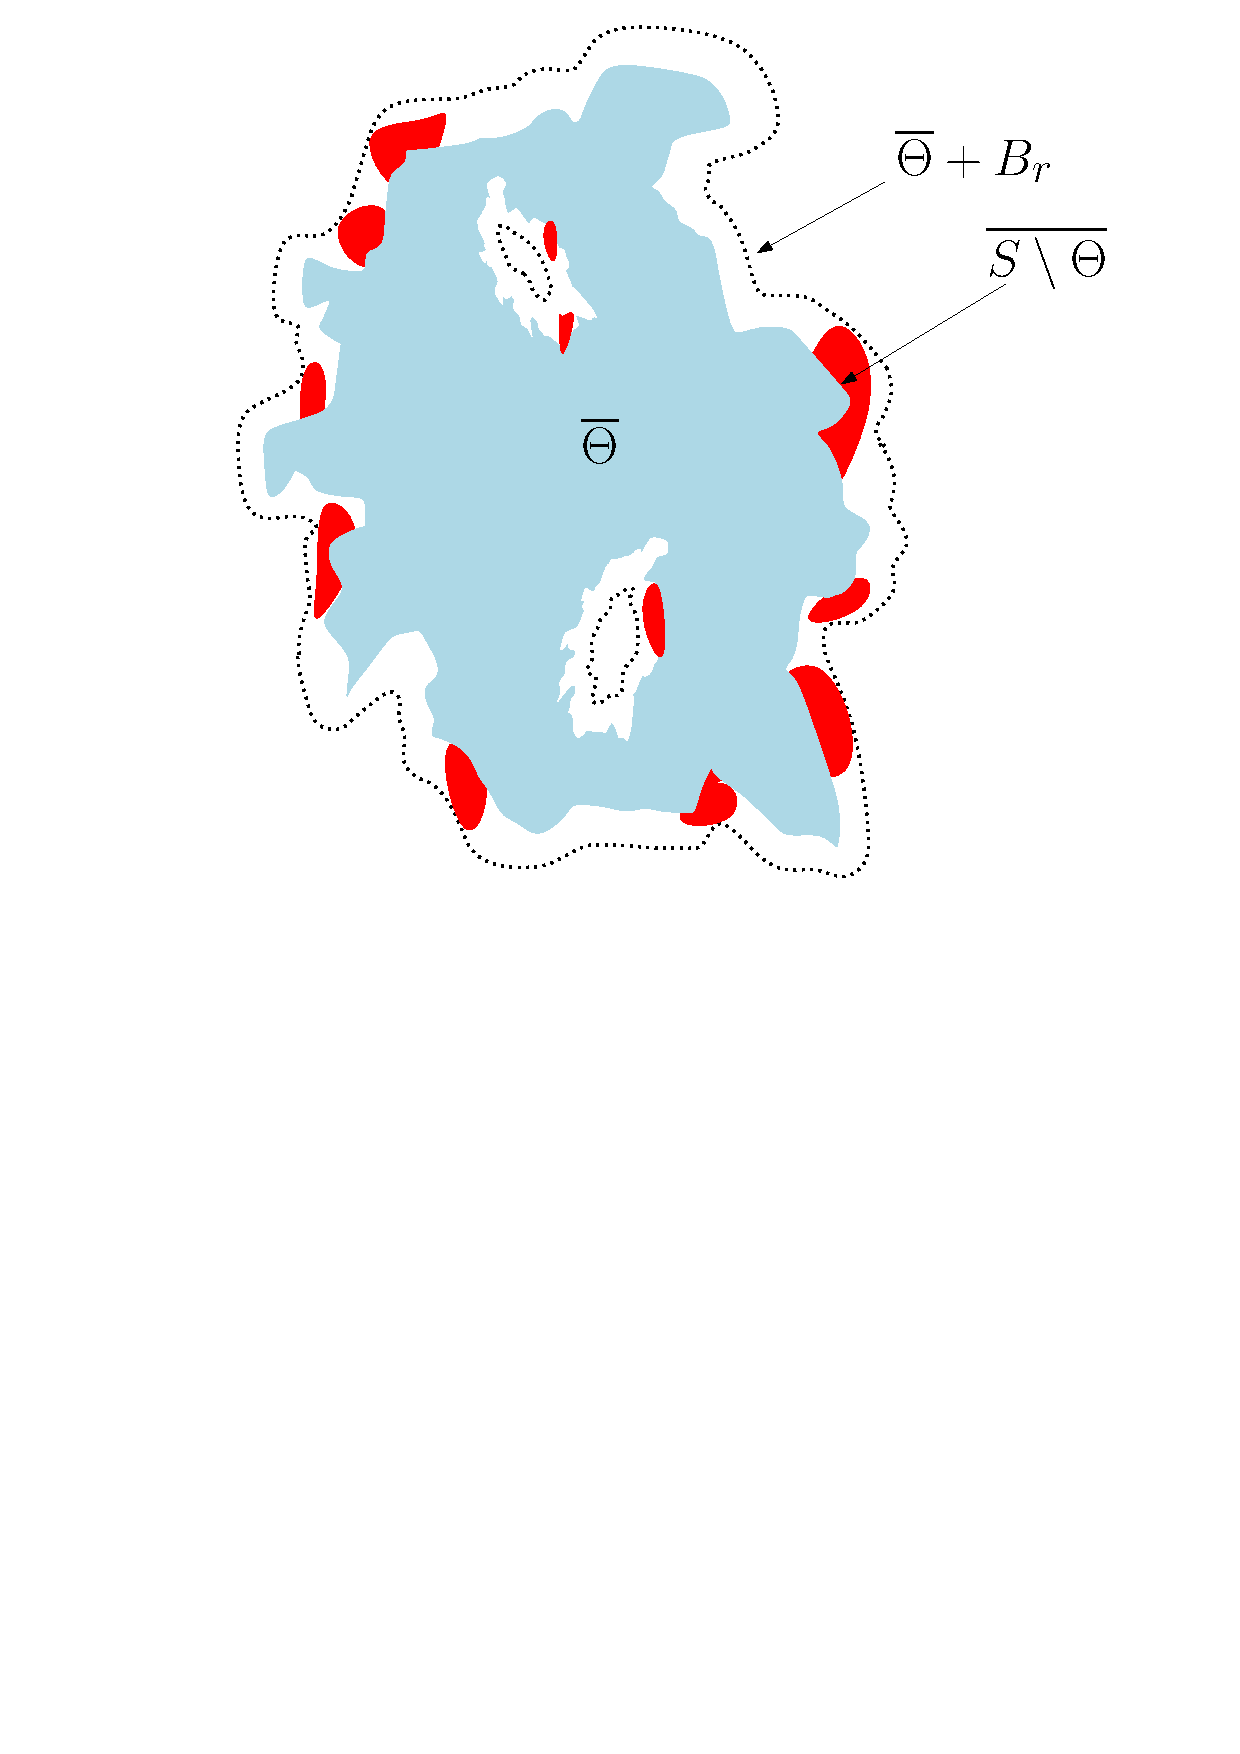
\includegraphics[width=0.5\textwidth]{Figures/fig-structure-graph-harmonic-measure.pdf}
		\caption{An illustration of the statement in Lemma \ref{lemma:constant-order-lower-bound}. The filled in cells corresponding to vertices in the cluster $\overline{\Theta}$ are shown in light blue and a neighborhood, $\overline{\Theta} + B_r$ is outlined by a dashed black line.  The set $\overline{S \setminus \Theta}$ is shown in red. Random walk started at a vertex in $\cl(\Theta)$
			is unlikely to exit ${\VGeps}(\overline{\Theta} + B_r)$ via paths which stay in $S$.}
		\label{fig:harmonic-measure-exit}
	\end{figure}
	
	
	
% CORRECTION [C26]: replace the proof of Lemma 6.8 by a target-scale short-window good-annulus construction and two-sided-shell amplification; this also repairs the [C5] kernel, Green-function, cell-size, stopping-time, and exponent-bookkeeping gaps.
\begin{proof}[Proof of Lemma \ref{lemma:constant-order-lower-bound-div}]
	As in the rest of this section, take the exponent $\beta^-$ in the
	statement to be a fixed deterministic choice allowed by Lemma
	\ref{lemma:volume-growth}, depending only on $\gamma$, and write
	$\beta=\beta^-$.  Fix once and for all
	\[
		0<\zeta<\frac12,
		\qquad
		\vartheta:=\frac{1+\zeta}{2}\in\left(\frac12,\frac34\right).
	\]
	Let $\kappa=\kappa(\gamma)>0$ be an exponent for which Lemma
	\ref{lemma:cell-size-estimate} gives the upper bound
	$\mathrm{diam}(\Heps{v})\leq \eps^\kappa$.  Let $\omega_{\rm G}$ be the
	exponent in Lemma \ref{lemma:greens-kernel-lower-bound}, and let
	$\alpha_{\rm c}$ and $\alpha_{\rm e}$ be the exponents in Lemmas
	\ref{lemma:mu_h-convergence} and \ref{lemma:exit-time-upper-bound},
	respectively.  We choose
	\begin{equation} \label{eq:c26-choice-omega}
		0<2\omega<\min\left\{
		\kappa,\omega_{\rm G},\alpha_{\rm e},
		\frac{\alpha_{\rm c}}{\beta},
		\frac{\alpha_{\rm e}}{\beta}
		\right\}.
	\end{equation}
	In particular, $\omega=\omega(\gamma)$.

	Let $C_{\rm G}=C_{\rm G}(\rho,\gamma)$ be the constant in Lemma
	\ref{lemma:greens-kernel-lower-bound}.  We use the freedom in the
	choice made in \eqref{eq:choice-of-constant-annulus} to take
	$\boldsymbol{c_0}$ still smaller, if necessary, so that
	\begin{equation} \label{eq:c26-choice-c0}
		\boldsymbol{c_0}<\frac1{48},
		\qquad
		C_{\rm G}^{-1}\log\frac1{8\boldsymbol{c_0}}-1\geq\frac12.
	\end{equation}
	This only changes the deterministic constant in Lemmas
	\ref{lemma:annulus-hit} and \ref{lemma:good-prevalance}.

	We first record three consequences of the results preceding the
	lemma.  They will be used simultaneously below.

	\medskip
	\noindent
	{\it Uniform lower volume bound.}
	By Lemma \ref{lemma:volume-growth} and the Borel--Cantelli lemma,
	there is an a.s. positive, $\sigma(h)$-measurable random variable
	$\boldsymbol t_*$ such that
	\begin{equation} \label{eq:c26-volume-all-scales}
		\mu_h(B_t(x))\geq c_{\rm v}t^\beta,
		\qquad x\in B_\rho,\quad 0<t<\boldsymbol t_*,
	\end{equation}
	where $c_{\rm v}=2^{-\beta}$.  Indeed, first apply Lemma
	\ref{lemma:volume-growth} at all sufficiently small dyadic radii.
	For an arbitrary $t$, choose a dyadic $q\in[t/2,t]$ and use
	$B_q(x)\subset B_t(x)$.  We decrease $\boldsymbol t_*$ so that all
	balls under consideration are contained in the range of Lemma
	\ref{lemma:volume-growth}.

	\medskip
	\noindent
	{\it Good radii in a short window.}
	There are a deterministic $C>0$ and an a.s. positive,
	$\sigma(h)$-measurable random variable $\boldsymbol d_*$ with the
	following property.  For every dyadic $d<\boldsymbol d_*$ and every
	\[
		z\in Z_d:=\left(B_{\rho-3d^\vartheta}\setminus
		B_{10d^\vartheta}\right)\cap\frac d{100}\Z^2,
	\]
	there is a measurably chosen radius
	\begin{equation} \label{eq:c26-short-window-radius}
		R_z(d)\in[d,d^\vartheta]\cap\{7^{-n}:n\in\N\}
	\end{equation}
	for which $E_{R_z(d)}(z;C)$ occurs.

	This is the proof of Lemma \ref{lemma:good-prevalance} with its
	list of radii restricted to the shorter window $[d,d^\vartheta]$.
	For completeness, we give the details.  Adding a constant to $h$
	multiplies every $\mu_h$-mass in the definition of $E_R(z;C)$ by
	the same factor.
	Consequently this event is determined by the restriction of $h$,
	viewed modulo additive constant, to
	\[
		\A_{(1-\boldsymbol{c_0})R,(2+\boldsymbol{c_0})R}(z)
		\subset \A_{3R/4,9R/4}(z).
	\]
	List the seven-adic radii in $[d,d^\vartheta]$ in decreasing
	order and continue the list below $d$ to obtain an infinite
	seven-adic sequence.
	% CORRECTION [C29]: justify translation since the quantum-cone field is not
	% itself translation invariant (in the replacement proof of [C26]; the printed paper has no translation step: "Apply Lemma ..., after translating by $z$, ...").
	For this fixed $z$, modulo an additive constant we may write
	\[
	h(z+\cdot)=\widetilde h^\C+\phi_z,
	\qquad
	\phi_z(w):=-\gamma\log|z+w|,
	\]
	where $\widetilde h^\C$ is a whole-plane GFF modulo additive constant.
	All of the annuli under consideration avoid $-z$, so $\phi_z$ is a
	deterministic continuous function on their union.  Adding $\phi_z$
	induces an invertible map on each annular field modulo additive constant.
	Consequently the translated events satisfy the hypotheses of
	Lemma \ref{lemma:annulus-iterate}, with the same marginal probability
	lower bound and the same constants.

	We therefore apply Lemma \ref{lemma:annulus-iterate} to the translated
	events, with scale radii
	$3R$, annular parameters $1/4$ and $3/4$, and
	\[
		\alpha_0:=\frac{10\log 7}{1-\vartheta}.
	\]
	We use the conclusion only for the first $K(d)$ terms, namely the
	radii which belong to $[d,d^\vartheta]$.
	Choose the probability threshold furnished by that lemma, and then
	choose $C$ by Lemma \ref{lemma:annulus-hit}.  The hypotheses of
	Lemma \ref{lemma:annulus-hit} hold for every $z\in Z_d$ and every
	$R\in[d,d^\vartheta]$: namely,
	$B_{3R}(z)\subset B_\rho$ and
	$\dist(\A_{R/3,3R}(z),\{0\})\geq 7d^\vartheta\geq R/100$.
	They also hold for every radius in the continuation below $d$, since
	such a radius is no larger than $d$.
	The number $K(d)$ of candidate radii satisfies
	\[
		K(d)\geq\frac{(1-\vartheta)\log(1/d)}{\log 7}-2.
	\]
	Consequently the probability that no candidate radius is good at a
	fixed $z$ is at most $C_1d^{10}$.  Since $|Z_d|\leq C_2d^{-2}$,
	the probability that some $z\in Z_d$ has no good radius is at most
	$C_3d^8$.  Summing over dyadic $d$ and applying Borel--Cantelli gives
	$\boldsymbol d_*$.  We decrease this cutoff by a deterministic amount,
	if necessary, so that the finite list in $[d,d^\vartheta]$ is nonempty
	for every dyadic $d<\boldsymbol d_*$.  Choosing, for example, the first
	good radius in that list gives the asserted measurable selection.

	\medskip
	\noindent
	{\it Conversion of the corrected annulus kernel.}
	For $R<1$, $z\in\C$, set
	\[
		m_R(z):=\inf_{w\in\A_{R,2R}(z)}
		\mu_h(B_{\boldsymbol{c_0}R}(w)).
	\]
	There is a deterministic $C_0=C_0(\rho,\gamma)>0$ such that, on
	$E_R(z;C)$, the following holds.  If
	$F\subset\A_{R,2R}(z)$ is Borel, $v\in\A_{R,2R}(z)$, and
	$|u-v|\leq R$ for every $u\in F$, then
	\begin{equation} \label{eq:c26-absolute-potential}
		\int_F\left(\log\frac1{|u-v|}+1\right)d\mu_h(u)
		\leq C_0\left(1+\log\frac1R\right)m_R(z).
	\end{equation}
	To see this, write
	$K_R(u,v)=\log(R/|u-v|)+1$.  If $\nu_R$ is normalized arclength
	measure on $\partial B_{3R/2}(z)$, then the mean-value property for
	$\log|\cdot|$ gives, for $u\in\A_{R,2R}(z)$,
	\[
		\int K_R(u,v)d\nu_R(v)
		=1+\log\frac{R}{\max\{|u-z|,3R/2\}}
		\geq 1-\log2.
	\]
	Since $K_R\geq1-\log4$ on the product of the annulus with
	itself and $\mu_h$ is finite on compact sets, we may apply Fubini
	after adding the constant $\log4-1$.  Averaging the defining
	inequality for $E_R(z;C)$ therefore yields
	\begin{equation} \label{eq:c26-annulus-mass}
		\mu_h(\A_{R,2R}(z))
		\leq\frac{C}{1-\log2}m_R(z).
	\end{equation}
	For the fixed $v$ in the claim, $K_R\geq1$ on $F$, whereas
	$K_R\geq1-\log4$ on the whole annulus.  Hence
	\begin{align*}
		\int_F K_R(u,v)d\mu_h(u)
		&=\int_{\A_{R,2R}(z)}K_R(u,v)d\mu_h(u)
		-\int_{\A_{R,2R}(z)\setminus F}K_R(u,v)d\mu_h(u)\\
		&\leq C m_R(z)+(\log4-1)\mu_h(\A_{R,2R}(z))
		\leq C_4m_R(z),
	\end{align*}
	by \eqref{eq:c26-annulus-mass}.  Adding
	$\log(1/R)\mu_h(F)$ and again using
	\eqref{eq:c26-annulus-mass} proves
	\eqref{eq:c26-absolute-potential}.  This is the point at which the
	scale-invariant kernel from correction \textup{[C5]} is used.

	We now specify the high-probability event for the map.  Put
	\[
		h_\eps:=\sup\{\mathrm{diam}(\Heps{v}):\Heps{v}\cap B_\rho\neq\emptyset\}.
	\]
	Intersect the simultaneous events in Lemmas
	\ref{lemma:cell-size-estimate}, \ref{lemma:mu_h-convergence},
	\ref{lemma:greens-kernel-lower-bound}, and
	\ref{lemma:exit-time-upper-bound}.  Their intersection has
	probability tending to one as $\eps\to0$.  By
	\eqref{eq:c26-choice-omega}, for all sufficiently small deterministic
	$\eps$, on this event, whenever $r\geq10\eps^\omega$ and $d$ is
	dyadic with $r^2\leq d<2r^2$, we have
	\begin{equation} \label{eq:c26-mesh-preparation}
		\begin{gathered}
		 \eps\leq8\boldsymbol{c_0},\qquad
		 h_\eps\leq\frac{\boldsymbol{c_0}d}{100},
		 \qquad \eps^{\alpha_{\rm e}}\leq\frac d{100},
		 \qquad \eps^{\omega_{\rm G}}\leq\frac d4,\\
		 \eps^{\alpha_{\rm c}}
		 \leq\frac{c_{\rm v}\boldsymbol{c_0}^\beta}{8}d^\beta,
		 \qquad
		 \eps^{\alpha_{\rm e}}
		 \leq c_{\rm v}4^{-\beta}d^\beta.
		\end{gathered}
	\end{equation}
	All of these inequalities are uniform over $r$ in the indicated
	range.  For example, $d\geq r^2\geq100\eps^{2\omega}$, and the
	strict exponent inequalities in \eqref{eq:c26-choice-omega} absorb
	the fixed constants in \eqref{eq:c26-mesh-preparation}; the first
	inequality there follows by taking $\eps$ deterministically small.

	Choose
	\begin{equation} \label{eq:c26-choice-s1}
		0<s_1\leq\min\left\{\frac12,
		\frac{c_{\rm v}\boldsymbol{c_0}^\beta}{8}\right\}.
	\end{equation}
	We next prove the local random-walk estimate which will be applied at
	each shell.

	\medskip
	\noindent
	{\it One good-annulus test.}
	Suppose that $r^2\leq d\leq R\leq d^\vartheta$, that
	$E_R(z;C)$ occurs, that $B_{3R}(z)\subset B_\rho$, and that
	\[
		b\in\VGeps(\partial B_{4R/3}(z)).
	\]
	Write $x=\eta(b)$ and set
	\[
		D:=B_{R/4}(x),
		\qquad D_0:=B_{\boldsymbol{c_0}R}(x),
		\qquad m_0:=\mu_h(D_0).
	\]
	We also suppose that $d^\vartheta\leq r/4000$ and that all the
	radii in this display are below $\boldsymbol t_*$.  Let
	\[
		\tau_D:=\inf\{n\geq0:X_n^{b,\eps}\notin
		(\VGeps(D)\setminus\VGeps(\partial D))\},
		\qquad
		V:=\sum_{0\leq n<\tau_D}
		1\{X_n^{b,\eps}\notin A\}.
	\]
	We claim that, for a deterministic $q_0=q_0(\rho,\gamma)>0$,
	\begin{equation} \label{eq:c26-one-test}
		\P[V\geq1\mid h,\eta]
		\geq\frac{q_0}{(1+\log(1/r))^2}.
	\end{equation}

	First, $D_0\subset B_r(x)$ since $R\leq d^\vartheta\leq r/4000$,
	and $R\geq r^2$.  Moreover,
	$h_\eps\leq\boldsymbol{c_0}d/100\leq
	\boldsymbol{c_0}R/100$.  Since $x=\eta(b)$ belongs to the cell of
	$b$, that cell is contained in $D$; and a cell which meets $D_0$ is
	contained in $B_{\boldsymbol{c_0}R+h_\eps}(x)\subset D$.  Hence
	the cell of $b$ and every cell in $\VGeps(D_0)$ belong to
	$\VGeps(D)\setminus\VGeps(\partial D)$.  Hence the sparsity
	hypothesis on $A$, \eqref{eq:c26-volume-all-scales},
	\eqref{eq:c26-mesh-preparation}, and
	\eqref{eq:c26-choice-s1} give
	\begin{align}
		|\VGeps(D_0)\setminus A|
		&\geq \eps^{-1}
		\left(m_0-\eps^{\alpha_{\rm c}}-s_1r^{2\beta}\right)
		\notag\\
		&\geq \frac12\eps^{-1}m_0.
		\label{eq:c26-target-count}
	\end{align}
	Indeed, $m_0\geq c_{\rm v}\boldsymbol{c_0}^\beta R^\beta$,
	$r^{2\beta}\leq R^\beta$, and the first line is Lemma
	\ref{lemma:mu_h-convergence} with the function equal to one.

	If $b'\in\VGeps(D_0)$, then
	$b'\in\VGeps(B_{R/12}(x))$ by
	\eqref{eq:c26-choice-c0}.  Furthermore, choosing a point of
	$\Heps{b'}\cap D_0$ and using
	\eqref{eq:c26-mesh-preparation},
	\[
		|\eta(b')-x|\leq2\boldsymbol{c_0}R.
	\]
	We check explicitly the hypotheses of Lemma
	\ref{lemma:greens-kernel-lower-bound} for the ball $D=B_{R/4}(x)$.
	By \eqref{eq:c26-mesh-preparation}, $R/4\geq d/4\geq
	\eps^{\omega_{\rm G}}$.  Also $B_{3R}(z)\subset B_\rho$ and
	$\left||x-z|-4R/3\right|\leq h_\eps$ give
	\[
		\dist(x,\partial B_\rho)\geq
		3R-\frac43R-h_\eps>\frac R4\geq
		\eps^{\omega_{\rm G}},
	\]
	so $b\in\VGeps(B_{\rho-\eps^{\omega_{\rm G}}})$ and
	$R/4\leq\dist(x,\partial B_\rho)$.  Finally,
	$b'\in\VGeps(B_{R/12}(x))$, and
	\[
		\left(\frac{R/4}{|x-\eta(b')|}\right)\wedge\eps^{-1}
		\geq\frac1{8\boldsymbol{c_0}}
	\]
	by the preceding distance estimate and
	$\eps\leq8\boldsymbol{c_0}$.  The lemma therefore gives
	\begin{equation} \label{eq:c26-green-half}
		\Gr{{\eps}}{D}(b,b')
		\geq C_{\rm G}^{-1}\log\frac1{8\boldsymbol{c_0}}-1
		\geq\frac12.
	\end{equation}
	Consequently, by the exact pre-exit Green-function identity,
	\begin{equation} \label{eq:c26-first-moment}
		\E[V\mid h,\eta]
		\geq\frac14\eps^{-1}m_0.
	\end{equation}

	Since the cell of $b$ meets $\partial B_{4R/3}(z)$,
	\[
		\left||x-z|-\frac43R\right|\leq h_\eps.
	\]
	It follows from \eqref{eq:c26-mesh-preparation} that
	\begin{equation} \label{eq:c26-ball-in-annulus}
		B_{R/4+\eps^{\alpha_{\rm e}}}(x)
		\subset\A_{R,2R}(z).
	\end{equation}
	Indeed, the inner and outer radial bounds are respectively
	$(4/3-1/4-2/100)R=319R/300>R$ and
	$(4/3+1/4+2/100)R=481R/300<2R$.
	The same estimates put $D$ in this annulus, and if $u$ belongs to
	the left side of \eqref{eq:c26-ball-in-annulus} and $v\in D$, then
	$|u-v|<R$.  Also $x\in\A_{R,2R}(z)$, so $m_R(z)\leq m_0$.
	The mass hypothesis in Lemma \ref{lemma:exit-time-upper-bound} holds
	because
	\[
		\mu_h(D)\geq c_{\rm v}(R/4)^\beta
		\geq c_{\rm v}4^{-\beta}d^\beta
		\geq\eps^{\alpha_{\rm e}}.
	\]
	Using \eqref{eq:c26-absolute-potential} in that lemma with $N=2$
	therefore gives
	\begin{equation} \label{eq:c26-second-moment}
		\E[V^2\mid h,\eta]
		\leq\E[\tau_D^2\mid h,\eta]
		\leq C_5\eps^{-2}
		\left(1+\log\frac1R\right)^2m_0^2.
	\end{equation}
	The second moment method, \eqref{eq:c26-first-moment}, and
	\eqref{eq:c26-second-moment} imply
	\[
		\P[V\geq1\mid h,\eta]
		\geq\frac{q_*}{(1+\log(1/R))^2}
	\]
	for some $q_*\in(0,1)$, after decreasing the constant if
	necessary.  Finally, $R\geq d\geq r^2$, so
	$1+\log(1/R)\leq2(1+\log(1/r))$ after decreasing the deterministic
	upper cutoff for $r$.  This proves \eqref{eq:c26-one-test}, with
	$q_0=q_*/4$.

	\medskip
	\noindent
	{\it Two-sided shells.}
	We now fix $s_0\in(0,1)$.  Choose a deterministic
	$r_0=r_0(s_0,\rho,\gamma)>0$ so small that the following hold for
	every $0<r\leq r_0$.  If $d$ is the dyadic number determined by
	\begin{equation} \label{eq:c26-base-scale}
		r^2\leq d<2r^2
	\end{equation}
	and $s=d^\vartheta$, then
	\begin{equation} \label{eq:c26-geometric-cutoffs}
		\begin{gathered}
		 s\leq r/4000,\qquad r\leq\min\{e^{-1},\rho/100\},\\
		 10s+2d/100<s_0,\\
		 \rho/2+0.55r+2d/100+3s<\rho,
		\end{gathered}
	\end{equation}
	Such an $r_0$ exists since
	$s\leq2^\vartheta r^{1+\zeta}=o(r)$.  We will decrease $r_0$
	once more at the end of the proof to obtain the numerical bound
	$s_2=1/2$.

	Set
	\begin{equation} \label{eq:c26-random-cutoff}
		\boldsymbol\delta
		:=r_0\wedge\sqrt{\boldsymbol d_*/4}
		\wedge
		\left(\frac{\boldsymbol t_*}{2^{\vartheta+1}}
		\right)^{1/(2\vartheta)}.
	\end{equation}
	This is positive and $\sigma(h)$-measurable.  Fix
	$r\in[10\eps^\omega,\boldsymbol\delta]$, an admissible $\Theta$ and
	$A$, and
	\[
		a\in\VGeps(\partial(\overline\Theta+B_{r/2})).
	\]
	For the dyadic $d$ in \eqref{eq:c26-base-scale} and
	$s=d^\vartheta$, the definition of $\boldsymbol\delta$ gives
	\begin{equation} \label{eq:c26-cutoff-consequences}
		d<\boldsymbol d_*,
		\qquad s<\boldsymbol t_*/2,
		\qquad s\leq r/4000.
	\end{equation}
	Indeed, $d<2r^2\leq\boldsymbol d_*/2$ and
	$s<2^\vartheta r^{2\vartheta}\leq\boldsymbol t_*/2$.
	Thus the short-window selector and all lower volume bounds used below
	are available at every selected radius.

	Let $\mathcal F_n$ be the natural filtration of the walk.  Write
	\[
		K:=\overline\Theta,
		\qquad
		U:=\VGeps(K+B_r)\setminus\Theta,
		\qquad
		\tau:=\inf\{n\geq0:X_n^{a,\eps}\notin U\},
	\]
	and put $f(x)=\dist(x,K)$.  The starting cell meets
	$\{f=r/2\}$, so it intersects $K+B_r$ and cannot correspond to a
	vertex of $\Theta$; hence $a\in U$.  The set $U$ is finite: indeed,
	the properness of the space-filling curve implies that a bounded
	Euclidean set meets only finitely many $\eps$-cells.  Since the
	map is connected, simple random walk exits every finite vertex set
	almost surely (from each vertex choose a finite path out of the set
	and iterate the resulting uniform positive exit probability).  Thus
	$\tau<\infty$ almost surely.  With the exit-through convention used in
	the statement, the bad event is
	\begin{equation} \label{eq:c26-bad-event}
		\mathcal B:=\{X_n^{a,\eps}\in A\text{ for every }0\leq n<\tau\}.
	\end{equation}

	For $d,s$ as above, let
	\[
		N:=\left\lfloor\frac r{400s}\right\rfloor,
		\qquad \lambda_j:=20js,
		\qquad
		\Sigma_j:=\left\{x:\left|f(x)-\frac r2\right|=\lambda_j\right\},
		\quad 1\leq j\leq N.
	\]
	By \eqref{eq:c26-geometric-cutoffs},
	\begin{equation} \label{eq:c26-number-shells}
		20s\leq\lambda_j\leq r/20,
		\qquad
		N\geq c_Nr^{-\zeta},
		\qquad c_N:=2^{-\vartheta}/800.
	\end{equation}
	In particular, every $\Sigma_j$ is contained in the band
	$0.45r\leq f\leq0.55r$.

	The starting cell meets $\{f=r/2\}$.  Hence every point of this cell
	has $|f-r/2|\leq h_\eps<\lambda_1$.  Define
	\[
		C_j:=\inf\{n\geq0:\Heps{X_n^{a,\eps}}\cap\Sigma_j\neq\emptyset\}.
	\]
	On $\mathcal B$, each $C_j$ is strictly smaller than $\tau$.  Indeed,
	consecutive cells intersect, so the union of the cells visited from
	time zero through time $\tau$ is connected.  At time $\tau$ either
	$X_\tau^{a,\eps}\in\Theta$, in which case its cell is contained in
	$K$ and $f=0$ there, or
	$X_\tau^{a,\eps}\notin\VGeps(K+B_r)$, in which case $f\geq r$ on
	its cell.  The continuous image of the connected union under
	$|f-r/2|$ therefore contains $[0,r/2]$.  The terminal cell itself
	meets none of the sets $\Sigma_j$, since on it either $f=0$ or
	$f\geq r$, while $\lambda_j<r/2$.  Hence every level $\lambda_j$
	is reached before time $\tau$.  More generally,
	\begin{equation} \label{eq:c26-shell-order}
		C_{j+1}<\tau\quad\Longrightarrow\quad C_j<C_{j+1}.
	\end{equation}
	The strictness follows because one cell cannot meet two successive
	shells, whose levels are separated by $20s$, whereas
	$h_\eps<s/100$.

	Let $Q_d$ denote a deterministic nearest-point rounding map onto
	$(d/100)\Z^2$.  On $\{C_j<\infty\}$, set
	\[
		x_j:=\eta(X_{C_j}^{a,\eps}),
		\qquad z_j:=Q_d(x_j).
	\]
	Choose $y_j\in\Heps{X_{C_j}^{a,\eps}}\cap\Sigma_j$.  Then
	\[
		\dist(z_j,\Sigma_j)
		\leq |z_j-x_j|+|x_j-y_j|
		\leq\frac{2d}{100}.
	\]
	Since $B_{s_0}\subset K$ and $K\Subset B_{\rho/2}$,
	\[
		|y_j|\geq s_0,
		\qquad
		|y_j|\leq\rho/2+0.55r.
	\]
	Together with \eqref{eq:c26-geometric-cutoffs}, this implies
	\[
		z_j\in Z_d.
	\]
	We may therefore define
	\[
		R_j:=R_{z_j}(d)
	\]
	on $\{C_j<\infty\}$; choose fixed deterministic defaults for
	$x_j,z_j,R_j$ on $\{C_j=\infty\}$.  The selected radius is good,
	and
	\begin{equation} \label{eq:c26-R-range}
		r^2\leq d\leq R_j\leq s.
	\end{equation}
	Consequently
	\begin{equation} \label{eq:c26-center-near-shell}
		\dist(z_j,\Sigma_j)\leq\frac{2d}{100}
		\leq\frac{R_j}{50}.
	\end{equation}
	For every $u$ in the cell at time $C_j$,
	$|u-z_j|\leq|u-x_j|+|x_j-z_j|\leq2d/100\leq R_j/50$.
	Thus the whole cell at time $C_j$ is contained in
	$B_{R_j/50}(z_j)$.

	Since every cell is connected, for every Euclidean ball $B$ one has
	\[
		\{v:\Heps{v}\subset B\}
		=\VGeps(B)\setminus\VGeps(\partial B).
	\]
	On $\{C_j<\infty\}$ define
	\[
		T_j:=\inf\left\{n\geq C_j:
		\Heps{X_n^{a,\eps}}\not\subset B_{4R_j/3}(z_j)\right\},
	\]
	and set $T_j=\infty$ on $\{C_j=\infty\}$.  This is a stopping
	time.  The cell at time $C_j$ is contained in the displayed ball, so
	$T_j>C_j$.  The set of cells contained in a bounded ball is finite,
	and simple random walk exits every finite vertex set almost surely;
	hence $T_j<\infty$ whenever $C_j<\infty$.  At time $T_j$ the exit
	cell intersects the preceding cell, which is contained in the ball,
	but is not itself contained in the ball.  Since cells are connected,
	\begin{equation} \label{eq:c26-boundary-start}
		X_{T_j}^{a,\eps}\in
		\VGeps(\partial B_{4R_j/3}(z_j)).
	\end{equation}
	The measurability assertion follows since $z_j,R_j$ are
	$\mathcal F_{C_j}$-measurable.  On $\{T_j<\infty\}$ put
	\[
		b_j:=X_{T_j}^{a,\eps},
		\qquad x'_j:=\eta(b_j),
		\qquad D_j:=B_{R_j/4}(x'_j),
	\]
	and define
	\[
		L_j:=\inf\{n\geq T_j:X_n^{a,\eps}\notin
		(\VGeps(D_j)\setminus\VGeps(\partial D_j))\}.
	\]
	Set $L_j=\infty$ on $\{T_j=\infty\}$.  Since
	$x'_j\in\Heps{b_j}$ and $h_\eps\leq R_j/100$, the cell of
	$b_j$ is contained in $D_j$.  Thus $L_j>T_j$ whenever
	$T_j<\infty$.  The vertex set $\VGeps(D_j)$ is finite, so
	$L_j<\infty$ whenever $T_j<\infty$.  Every cell used from time
	$C_j$ through time $L_j$,
	including the exit cell at time $L_j$, is contained in
	$B_{2R_j}(z_j)$.  Indeed, before $T_j$ the cells are contained in
	$B_{4R_j/3}(z_j)$; the cell at $T_j$ meets its boundary; the cells
	strictly before $L_j$ are contained in $D_j$; and the cell at
	time $L_j$ meets $\partial D_j$.  The latter follows because it
	intersects the preceding cell in $D_j$ and is not an interior
	vertex of $D_j$.  Using $h_\eps\leq R_j/100$ gives
	\[
		\frac43R_j+h_\eps+\frac14R_j+2h_\eps<2R_j.
	\]
	By \eqref{eq:c26-center-near-shell}, every point of these cells
	satisfies
	\begin{equation} \label{eq:c26-test-near-shell}
		\left|\left|f-\frac r2\right|-\lambda_j\right|<3s.
	\end{equation}
	Since consecutive shell levels are separated by $20s$, we obtain the
	pathwise ordering
	\begin{equation} \label{eq:c26-test-order}
		C_{j+1}<\tau
		\quad\Longrightarrow\quad
		C_j<T_j<L_j<C_{j+1},
		\qquad 1\leq j<N.
	\end{equation}
	In fact, for every $j$, $C_j<\tau$ implies $L_j<\tau$.  Indeed,
	\eqref{eq:c26-test-near-shell} and $\lambda_j\leq r/20$ imply that
	every whole cell used by any test satisfies
	\begin{equation} \label{eq:c26-test-inside-U}
		0.449r<f<0.551r.
	\end{equation}
	Such a cell lies in $(K+B_r)\setminus K$, so its vertex belongs to
	$U$.

	We can now apply the one-test estimate.  On $\{T_j<\tau\}$,
	\eqref{eq:c26-boundary-start}, \eqref{eq:c26-R-range}, the goodness
	of $R_j$, and the preceding containment verify all the hypotheses of
	\eqref{eq:c26-one-test}.  The strong Markov property at $T_j$ gives
	\begin{equation} \label{eq:c26-conditional-test}
		\P\left[
		\left.\exists n\in[T_j,L_j):X_n^{a,\eps}\notin A
		\,\right|\mathcal F_{T_j},h,\eta\right]
		\geq q(r):=\frac{q_0}{(1+\log(1/r))^2}
	\end{equation}
	on $\{T_j<\tau\}$.  By \eqref{eq:c26-test-inside-U}, every hit in
	\eqref{eq:c26-conditional-test} is a visit to $U\setminus A$ before
	$\tau$.

	For $1\leq j\leq N$, define
	\[
		\mathcal P_j:=\{T_j<\tau,\ X_n^{a,\eps}\in A\text{ for all }n<T_j\},
	\]
	and
	\[
		\mathcal Q_j:=\{X_n^{a,\eps}\in A\text{ for all }T_j\leq n<L_j\}.
	\]
	Then $\mathcal P_j\in\mathcal F_{T_j}$, and
	\eqref{eq:c26-conditional-test} implies
	\[
		\P[\mathcal Q_j\mid\mathcal F_{T_j},h,\eta]
		\leq1-q(r)
		\quad\text{on }\mathcal P_j.
	\]
	The pathwise ordering \eqref{eq:c26-test-order} gives
	\[
		\mathcal P_{j+1}\subset\mathcal P_j\cap\mathcal Q_j,
		\qquad j<N.
	\]
	Therefore, by conditional expectation,
	\[
		\P[\mathcal P_{j+1}\mid h,\eta]
		\leq(1-q(r))\P[\mathcal P_j\mid h,\eta].
	\]
	On the event $\mathcal B$, every shell is reached and every local
	test fails; in particular,
	$\mathcal B\subset\mathcal P_N\cap\mathcal Q_N$.  Iterating the last
	display and using the final test gives
	\begin{align}
		\P[\mathcal B\mid h,\eta]
		&\leq(1-q(r))^N\notag\\
		&\leq\exp\left[-\frac{c_*r^{-\zeta}}
		{(1+\log(1/r))^2}\right],
		\qquad c_*:=c_Nq_0>0.
		\label{eq:c26-amplified-bound}
	\end{align}
	No independence of the tests is used.

	Since
	$r^{-\zeta}/(1+\log(1/r))^2\to\infty$ as $r\to0$, choose a
	deterministic $r_{\rm amp}=r_{\rm amp}(\rho,\gamma)>0$ so that
	the right side of \eqref{eq:c26-amplified-bound} is at most $1/2$
	for every $0<r\leq r_{\rm amp}$.  Replace $r_0$ in
	\eqref{eq:c26-random-cutoff} by $r_0\wedge r_{\rm amp}$ and
	redefine $\boldsymbol\delta$ accordingly.  Thus the conclusion
	of the lemma holds with
	\[
		s_2=\frac12.
	\]
	The construction is simultaneous for every admissible
	$r,\Theta,A$, and starting vertex $a$ on the common event described
	above, whose probability tends to one as $\eps\to0$.  The random
	cutoff \eqref{eq:c26-random-cutoff} is $\sigma(h)$-measurable.

	Finally, although the statement places the choices of $s_1,s_2$
	after $s_0$, the proof gives the stronger dependence order: the
	constants $s_1$ in \eqref{eq:c26-choice-s1} and $s_2=1/2$ depend
	only on $(\rho,\gamma)$ and are chosen before $s_0$; only
	$\boldsymbol\delta$ depends on $s_0$.
\end{proof}
	\begin{figure}
		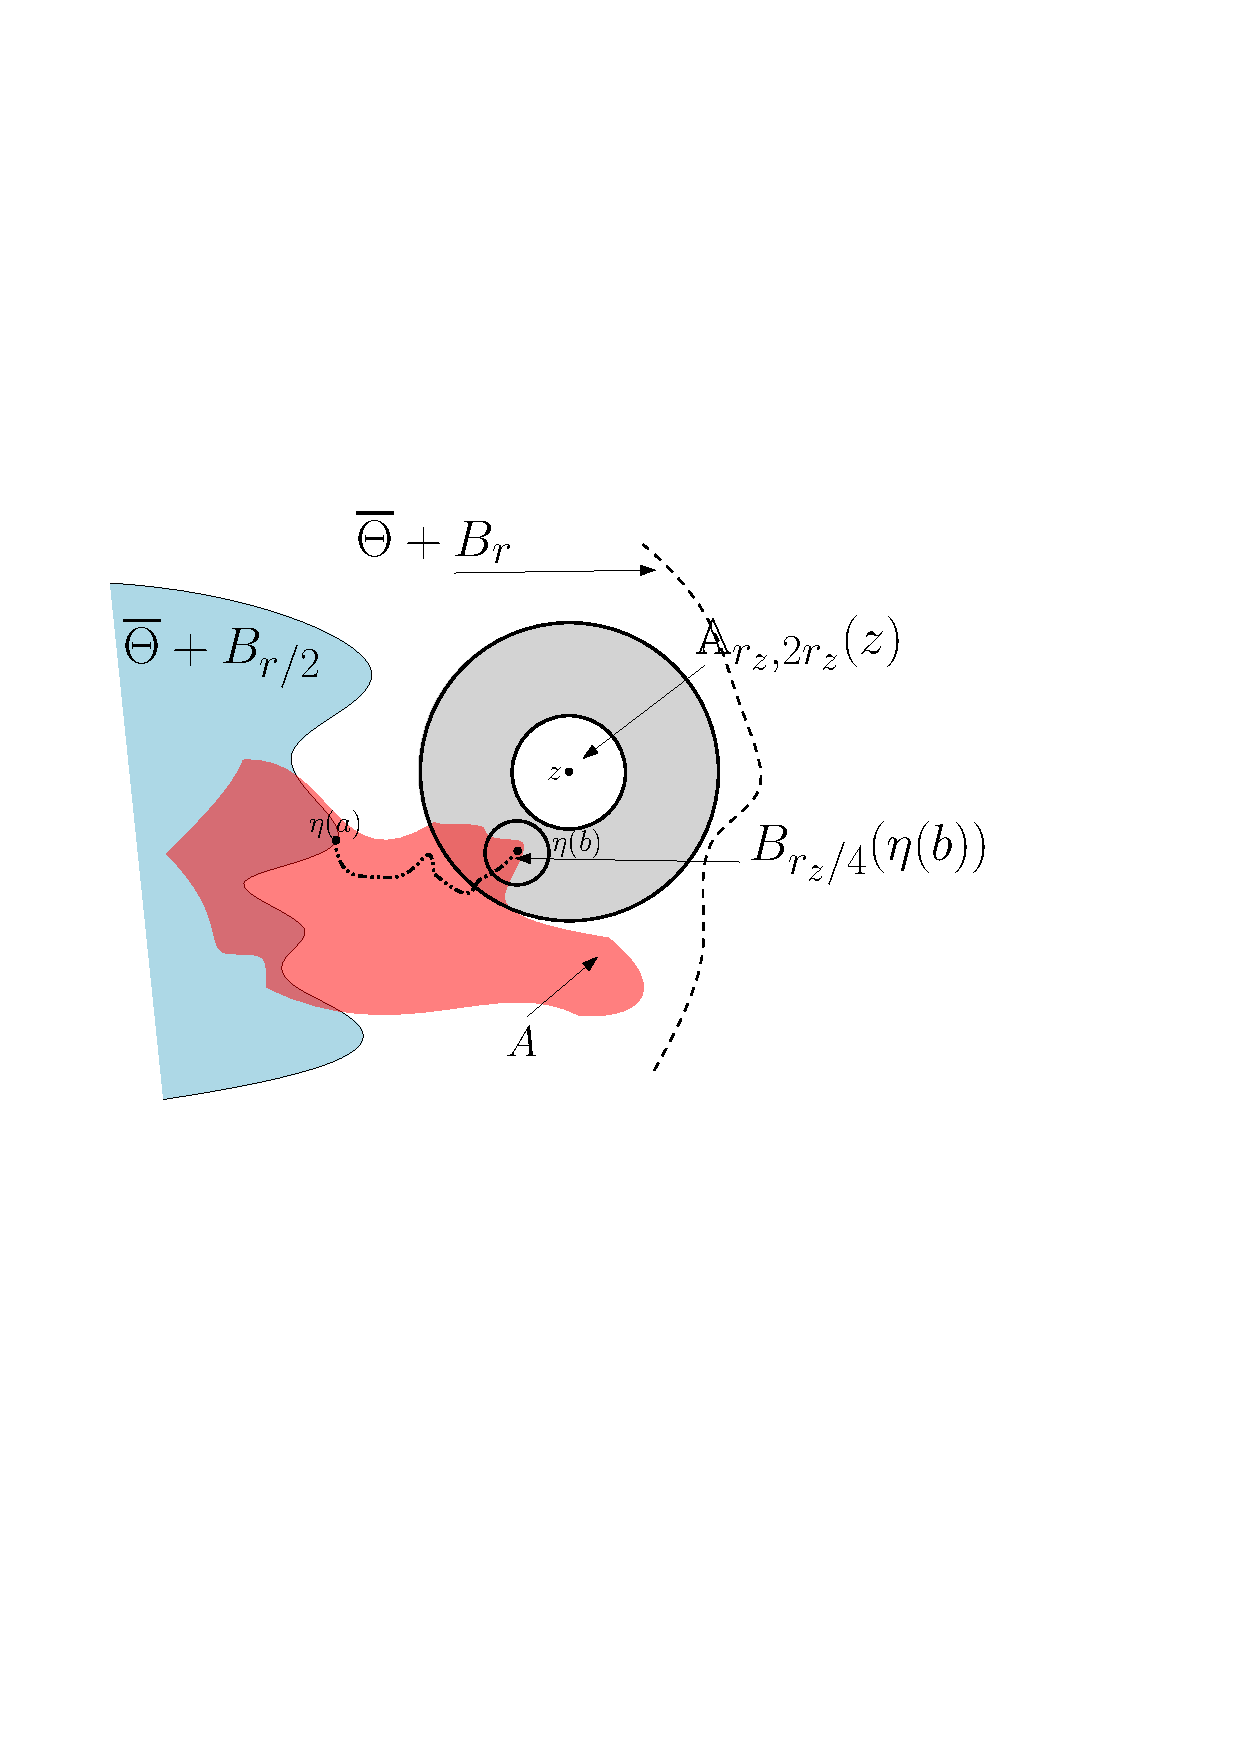
\includegraphics[width=0.5\textwidth]{Figures/fig-reduction-to-ball.pdf}
		\caption{Illustration of part of the proof of Lemma \ref{lemma:constant-order-lower-bound}; only parts of the sets are shown and aspect ratios are not drawn to scale.
			The set $\overline{\Theta} + B_{r/2}$ is shown in blue with a solid black boundary, 
			the boundary of $\overline{\Theta} + B_{r}$ is shown as a dashed black line.
			A good annulus $\A_{r_z, 2 r_z}(z)$ is shown in gray, an interior ball is outlined in black, and the set $A$ is shown 
			in light-red. A random walk started at $a$ must hit ${\VGeps}(B_{{(4/3)} r_{z}}(z))$ for some ${z} \in \mathbf{Z}$
			at a point $b \in {\VGeps}(\partial B_{{(4/3)} r_{z}}(z))$. The proof then reduces to showing a random walk started at $b$ with 
			probability bounded from below must exit 
			$A$ before exiting ${\VGeps}(B_{r_{z}/4}(b))$.} \label{fig:path-decomposition}
	\end{figure}	
	
	
	
	We next show that with exponentially high probability in $r$, if one starts $k \leq r^{2 \beta^-} {\eps}^{-1}$ walkers somewhere 
	in the closure of the current cluster $\cl(\Theta)$, then the number of walkers which are absorbed 
	before exiting ${\VGeps}(\overline\Theta + B_r)$ is at least a constant fraction of $k$. 
	The proof uses the constant-order lower bound given by Lemma \ref{lemma:constant-order-lower-bound} together with a concentration inequality for negative binomials. 
	The statement is a modification of \cite[Lemma 6]{duminil2013containing}. Note that \cite[Lemma 6]{duminil2013containing} is much stronger than what we have below, 
	but that stronger statement is not needed to complete the proof of the IDLA upper bound. For the statement, we recall the definition of the modified IDLA aggregate from Definition~\ref{def:stopped-idla}.
	
	\begin{lemma} \label{lemma:chance-of-being-absorbed}		
				% CORRECTION [C35]: the choice of $s_3$ follows $s_0$, as in Lemma 6.7 (E-c5-1); the proof below is unchanged.
		There exists deterministic $\omega = \omega(\gamma) > 0$ so that for each $s_0 \in (0,1)$, there exist $s_3 > 0$ and $s_4, s_5 \in (0,1)$ 
		and a random $\sigma(h)$-measurable $\boldsymbol{\delta} >0$ such that with probability approaching one as ${\eps}$ goes to zero, the following holds for $r \in [10 {\eps}^{\omega}, \boldsymbol{\delta}]$ 
		for all sets $\Theta \subset {\VGeps}$ 
		such that $\overline{\Theta} \Subset B_{\rho/2}$ and $B_{s_0} \subset \overline{\Theta}$ with $\overline{\Theta}$ as in \eqref{eq:vertex-scaling}:
		for each $k \leq s_5 r^{2 \beta^-} {\eps}^{-1}$ and $a_1, \ldots, a_{k} \in \cl(\Theta)$, 
		\[
		\P[ |A(\Theta; a_1, \ldots, a_{k} \to {\VGeps}(\overline{\Theta} + B_r)) \setminus \Theta| \leq s_4 k | h ,\eta] \leq \exp(-s_3 k).
		\]
	\end{lemma}
	
	\begin{proof}
		For $s_0 \in (0,1)$, let $\omega$, $s_1, s_2$ be as in Lemma \ref{lemma:constant-order-lower-bound} 
		and fix ${\eps}$ and $r \geq 10 {\eps}^{\omega}$ for which the event of Lemma \ref{lemma:constant-order-lower-bound}  occurs. Set $s_5 = \min(\frac{s_1}{s^{-1}_2 + C}, s_1)$ for a
		deterministic constant $C > 0$ from \eqref{eq:number-of-walkers-nb-bound} below.  Let $k \leq s_5 r^{2 \beta^-} {\eps}^{-1}$ and $a_1, \ldots, a_{k} \in \cl(\Theta)$
		% CORRECTION [C31]: match the statement and the subsequent argument (printed: $\in \Theta$).
		be given. 
		
		Start with the set $\Theta$ completely occupied and consider an infinite number of walkers each started at an arbitrary site in $\cl(\Theta)$ and stopped upon exiting ${\VGeps}(\overline\Theta + B_r)$. Let $\mathcal{N}(k_1)$ denote the number of such walkers 
		needed until $k_1$ walkers have been absorbed into the cluster. That is, $\mathcal N(k_1)$ counts the number of walkers needed
		until the aggregate has an additional $k_1$ walkers in ${\VGeps}(\overline\Theta + B_r) \setminus \Theta$. 
		
		We seek to iteratively apply Lemma \ref{lemma:constant-order-lower-bound}. Define $S_0 = \Theta$ and for each $k' \in \{1, \ldots, k_1\}$
		condition on the first $(k'-1)$ walkers to determine the current aggregate $S_{k'-1}$. 
		We then apply Lemma \ref{lemma:constant-order-lower-bound} with $S := S_{k'-1}$ to the $k'$-th walker under the conditional law given the first $(k'-1)$ 
		walkers. By the Markov property of IDLA this implies that
		\[
		\mathcal{N}(k_1) \leq \mathrm{NegBinom}(k_1, s_2), \quad \forall k_1 \leq s_1 r^{2 \beta^-} {\eps}^{-1}
		\]
		where $\mathrm{NegBinom}(k_1,s_2)$ denotes a random variable drawn from a negative binomial distribution with $n = k_1$ and $p = s_2$, sampled independently from $(h,\eta)$. 
		Therefore, by a concentration inequality for negative binomial random variables, for each $k_1 \leq s_1 r^{2 \beta^-} {\eps}^{-1}$, 
		% CORRECTION [C19] (author-approved 2026-11-10) Printed: \mathcal{N}(k_1) \leq (s_2^{-1}+C)k_1 here and \mathcal{N}(\cdot) \leq k in the next display.
		% Both tail events were reversed: the negative-binomial domination bounds the probability of needing too many walkers (with certain
		% absorption \mathcal{N}(m)=m, so the printed left side equals 1). The inclusive threshold in the conclusion is routine rounding.
		\begin{equation} \label{eq:number-of-walkers-nb-bound}
		\P[ \mathcal{N}(k_1) > (s_2^{-1} + C) k_1 | h, \eta] \leq \exp(-c k_1), \quad \mbox{for deterministic constants $C, c > 0$}.
		\end{equation}
		Thus, if we choose $k_1 = (s_2^{-1} + C)^{-1} \times k$, we have by our choice of $s_5$ and 
		\eqref{eq:number-of-walkers-nb-bound}, 
		\[
		\P\left[ \mathcal{N}((s_2^{-1} + C)^{-1} \times k) > k | h , \eta \right]  \leq \exp(-c k),
		\] 
		where the deterministic constant $c$ has changed compared to \eqref{eq:number-of-walkers-nb-bound}.
		By definition of $\mathcal{N}$, this implies the desired conclusion with $s_3 = c$ and $s_4 = (s_2^{-1} + C)^{-1}$.
	\end{proof}
	
	
	
	
	
	
	\subsection{Iteration} \label{subsec:iteration}
	We now prove a general bound on how far walkers can spread by iterating Lemma \ref{lemma:chance-of-being-absorbed}. 
	The iteration uses the Abelian property of IDLA and involves starting and stopping walkers which reach a certain distance
	of the current cluster. The proof is similar to that of \cite[Theorem 2]{duminil2013containing}.
	
	
	\begin{lemma}  \label{lemma:iterative-bound}
		There exists a deterministic exponent $\beta = \beta(\rho, \gamma) > 0$ and a constant $C = C(\rho, \gamma)>0$ so that 
		for each $s_0 \in (0,1)$ there exists a $\sigma(h)$-measurable random variable $\boldsymbol{\delta}_0$
		such that with probability approaching one as ${\eps} \to 0$,  for each $\overline{\Theta} \Subset B_{\rho/2}$ with $B_{s_0} \subset \Theta$ 
		and each $\delta_0 < \boldsymbol{\delta}_0$ the following is true. 
		The IDLA cluster started with  $\Theta$ completely occupied and
		$j \leq \lceil \delta_0 {\eps}^{-1} \rceil$ walkers at sites $\{a_1, \ldots, a_{j}\} \subset \cl(\Theta)$ 
		is contained in a $C \delta_0^\beta$ neighborhood of $\Theta$:
		\[
		A(\Theta; a_1, \ldots, a_{j}) \subset {\VGeps}(\Bdeltapp{C \delta_0^\beta}(\overline{\Theta})) \subset {\VGeps}(B_{\rho}).
		\]
	\end{lemma}
	\begin{proof}
		For $s_0 \in (0,1)$, let the parameters $\omega, s_3, s_4, s_5$ and random variable $\boldsymbol{\delta}$ be as in  Lemma \ref{lemma:chance-of-being-absorbed}.
		We truncate on the event of Lemma \ref{lemma:chance-of-being-absorbed} and fix an ${\eps}$. 
		Below we use the fact that Lemma \ref{lemma:chance-of-being-absorbed} is stated for {\it all}  choices of $\Theta$ satisfying the hypotheses and IDLA is a Markov process, 
		Lemma \ref{lemma:abelian-IDLA}. 	Throughout the proof we introduce several other events 
		which occur with probability approaching one as ${\eps} \to 0$ and will truncate on those events. 
		
		Let $\beta^-$ be as in Lemma \ref{lemma:volume-growth}.
		Let $\boldsymbol{\delta_0} = \boldsymbol{\delta_0}(\boldsymbol{\delta}, \rho, \gamma) < \boldsymbol{\delta}$ be such that $(\boldsymbol{\delta_0} s_5^{-1})^{1/2 \beta^-} \leq \boldsymbol{\delta}$, so that Lemma \ref{lemma:chance-of-being-absorbed} holds with $r \in ( 10 {\eps}^{\omega}, (\boldsymbol{\delta_0} s_5^{-1})^{1/2 \beta^-})$.  
		At the end of the proof, we reveal, in a deterministic fashion,  how small  $\boldsymbol{\delta_0}$ must be
		so that the final cluster is contained in ${\VGeps}(B_{\rho})$. Fix $\delta_0 < \boldsymbol{\delta_0}$. 
		
		
		Fix $\omega_0 \in (0,\omega)$ which we will choose in \eqref{eq:choice-of-omega0} below. 
		Set $\Theta^0 = \Theta$, $P_0 =\{a_1, \ldots, a_j\}$, 
		and for $k \geq 1$, inductively define (using the notation of Definition~\ref{def:stopped-idla})
		\[
		\begin{cases}
		\mbox{Current radius: } & r_k :=  \max\left( (|P_{k-1}| \times {\eps} \times s_5^{-1})^{1/{2 \beta^-}}, 10 {\eps}^{\omega_0} \right) \\
		\mbox{Current cluster: } & \Theta^{k} := A(\Theta^{k-1}; P_{k-1} \to {\VGeps}(\overline{\Theta^{k-1}} + B_{r_k})) \\
		\mbox{Stopped walkers: } & P_k := P(\Theta^{k-1}; P_{k-1} \to {\VGeps}(\overline{\Theta^{k-1}} + B_{r_k})).
		\end{cases}
		\]
		Define the stopping time
		\begin{equation} \label{eq:iterate-stop-time3}
		\tau_{{\eps},3} = \min \{ k \geq 0 : \overline{\Theta^{k}} \not \subset B_{\rho}\}.
		\end{equation}
		In the analysis below, we will truncate on a high probability event which ensures that $\tau_{{\eps},3}  =\infty$.
		
		Denote the first time there are fewer than 
		${\eps}^{-\omega_0}$ stopped walkers by 
		\begin{equation} \label{eq:iterate-stop-time2}
		\tau_{{\eps},2} = \min \left( \min \{ k \geq 0 : |P_k| \leq {\eps}^{-\omega_0}\}, \tau_{{\eps},3} \right)
		\end{equation}
		and the first time (before $\tau_{{\eps},2}$) that the current radius is less than $10 {\eps}^{\omega_0}$ by 
		\begin{equation}
		\tau_{{\eps},1} = \min \left( \min \{ k \geq 0 : r_k \leq 10 {\eps}^{\omega_0} \}, \tau_{{\eps},2} \right).
		\end{equation}
		By the Abelian property of IDLA, Lemma \ref{lemma:abelian-IDLA}, the distribution of the final IDLA cluster $A(\Theta; a_1, \ldots, a_{\lceil \delta_0 {\eps}^{-1} \rceil})$
		coincides with that of $\Theta^{\infty}$. Thus, it suffices to iteratively control how far the clusters $\Theta^{k}$ spread. In the first step, we control how far the aggregate spreads until 
		time $\tau_{{\eps},1}$, in the second, until time $\tau_{{\eps},2}$. In the third step, we control how far ${\eps}^{-\omega_0}$ walkers can spread.
		We show in the final step, after making $\boldsymbol{\delta_0}$ smaller in a deterministic way, that in fact we have $\tau_{{\eps},2} < \tau_{{\eps},3}$ and 
		$\tau_{{\eps},3} = \infty$. 
		
		Before proceeding, we note that by Lemma \ref{lemma:cell-size-estimate} (after truncating on another high probability event),  for each $\zeta > 0$, 
		\begin{equation} \label{eq:cell-size-estimate-local}
		\diam(H^{{\eps}}_a) \leq {\eps}^{2/(2+\gamma)^2 - \zeta} \quad \forall a \in {\VGeps}(B_{\rho}). 
		\end{equation}
		Choose $\zeta$ in a way which depends only on $\gamma$ and then choose $\omega_0$ small enough so that 
		\begin{equation} \label{eq:choice-of-omega0}
		{\eps}_0^{-\omega_0}  \times {\eps}_0^{2/(2+\gamma)^2 - \zeta} \leq {\eps}_0^{\omega_0/2} ,\quad \forall {\eps}_0 \in (0,1) .
		\end{equation}
		\medskip
		
		{\it Step 1: $t < \tau_{{\eps},1}$.} \\
		All of our parameter choices so far have been so that we can iteratively apply 
		Lemma \ref{lemma:chance-of-being-absorbed} for each $k \in \{1, \ldots, \tau_{{\eps},1}-1\}$ with $\Theta = \Theta^{k}$, 
		$r = r_k$, and $k = |P_{k-1}| \geq {\eps}^{-\omega_0}$.
		
		By \eqref{eq:cell-size-estimate-local} and \eqref{eq:choice-of-omega0} and the fact $r_k \geq 10 {\eps}^{\omega_0}$, there is a `shell' of additional vertices in
		$\Theta^{k}$ that are not in $\Theta^{k-1}$; that is, $\partial \Theta^{k} \cup \Theta^{k-1}$ is not connected. 
		Therefore, at least one walker is absorbed in each step and hence we have $\tau_{{\eps},1} \leq \tau_{{\eps},2} \leq {\eps}^{-1}$.
		Thus, by Lemma \ref{lemma:chance-of-being-absorbed} (with $s_3 > 0$ and $s_4 \in (0,1)$ from there)  and a union bound over all $k=1,\dots,\lfloor{\eps}^{-1} \rfloor$, 
		\begin{equation} \label{eqn:use-absorb}
		\P \left[ \exists k \in \{1, \ldots, \tau_{{\eps},1}-1\} : |P_k| \geq (1-s_4) |P_{k-1}| | h, \eta \right] \leq {\eps}^{-1} \exp(- s_3 {\eps}^{-\omega_0}).
		\end{equation}
		We henceforth truncate on the event in~\eqref{eqn:use-absorb}, which happens with probability tending to 1 as ${\eps}\to 0$
		to see that 	
		\begin{equation} \label{eq:good-event} 
		|P_k| \leq (1-s_4) |P_{k-1}|, \quad \forall k \in \{1, \ldots, \tau_{{\eps},1}-1\} .
		\end{equation}
		This implies that $|P_k| \leq (1-s_4)^k |P_0| \leq (1-s_4)^k \delta_0 {\eps}^{-1}$ for each $k\leq \tau_{{\eps},1}-1$. By the definition of $r_k$, this, in turn, implies that
		\begin{equation} \label{eq:good-event2} 
		r_k \leq (\delta_0\times (1-s_4)^{k-1} \times s_5^{-1})^{1/2\beta^-}, \quad \forall k \in \{1, \ldots, \tau_{{\eps},1}-1\} .
		\end{equation} 
		Therefore, 
		\begin{equation} \label{eq:bound-on-radii-sum}
		\sum_{k=1}^{\tau_{{\eps},1}-1} r_k \leq \sum_{k=1}^{\tau_{{\eps},1}-1} (\delta_0\times (1-s_4)^{k-1} \times s_5^{-1})^{1/2\beta^-} \leq C \times \delta_0^{1/2\beta^-} \times \frac{1}{1 - (1-s_4)^{1/2\beta^-}},
		\end{equation}
		where $C = C(s_5) > 0$ is deterministic. 
		\medskip
		
		
		{\it Step 2: $k \in [\tau_{{\eps},1}, \tau_{{\eps},2})$.} \\
		In this step we again apply Lemma \ref{lemma:chance-of-being-absorbed} for each $k \in \{\tau_{{\eps},1}, \ldots, \tau_{{\eps},2}\}$ 
		with the same choice of parameters as in Step 1 except now the radius is fixed $r_k = 10 {\eps}^{\omega_0}$. 
		Note that $r_k \geq (|P_{k-1}| \times {\eps} \times s_5^{-1})^{1/{2 \beta^-}}$ by definition and hence the conditions of Lemma \ref{lemma:chance-of-being-absorbed}
		are satisfied. 
		We show that 
		\begin{equation} \label{eq:time-upper-bound}
		\tau_{{\eps},2} \leq C \log {\eps}^{-1} + \tau_{{\eps},1}, \quad \mbox{for deterministic $C = C(s_4, \gamma) > 0$} 
		\end{equation}
		and hence 
		\begin{equation}
		\sum_{k=\tau_{{\eps},1}}^{\tau_{{\eps},2}} r_k \leq C \times {\eps}^{\omega_0} \times \log {\eps}^{-1}, \quad \mbox{for deterministic $C = C(s_4, \gamma) > 0$}.
		\end{equation}
		To see \eqref{eq:time-upper-bound}, we first use exactly the same argument as in Step 1 (and truncate on another event) to get that	
		\[
		|P_k| \leq (1-s_4) |P_{k-1}|, \quad \forall k \in \{\tau_{{\eps},1}, \ldots, \tau_{{\eps},2} \} .
		\]
		Hence, by the definition~\eqref{eq:iterate-stop-time2} of $\tau_{{\eps},2}$, 
		\[
		{\eps}^{-\omega_0} \leq |P_{\tau_{{\eps},2}-1}| \leq (1-s_4)^{\tau_{{\eps},2}- \tau_{{\eps},1}-1} {\eps}^{-1}
		\]
		which implies \eqref{eq:time-upper-bound} upon re-arranging. 
		\medskip
		
		{\it Step 3: $k \geq \tau_{{\eps},2}$.} \\
		It remains to control how far the remaining ${\eps}^{-\omega_0}$ walkers can go before being absorbed. 
		We do this crudely by appealing to the upper bound on the Euclidean diameter of cells in the mated-CRT map:
		by \eqref{eq:cell-size-estimate-local} and \eqref{eq:choice-of-omega0}
		we have that ${\eps}^{-\omega_0}$ walkers cannot go farther than Euclidean distance ${\eps}^{\omega_0/2}$ before being absorbed into the cluster,
		\begin{equation} \label{eq:distance-of-final-cluster}
		\dist(\overline{\Theta^{\infty}}, \overline{\Theta^{\tau_{{\eps},2}}}) < {\eps}^{\omega_0/2},
		\end{equation}
		since each walker occupies at least one cell.
		\medskip
		
		{\it Step 4: Reduce ${\eps}$ and $\boldsymbol{\delta_0}$ and conclude.} \\
		By combining Steps 1-3, the final aggregate $\overline{\Theta^{\infty}}$ is contained in $\overline{\Theta} + B_R$, where
		\[
		\begin{aligned}
		R &=  C \times \delta_0^{1/2\beta^-}  \quad \mbox{(by \eqref{eq:bound-on-radii-sum})} \\
		&+  C \times {\eps}^{\omega} \times \log {\eps}^{-1}  \quad \mbox{(by \eqref{eq:time-upper-bound})} \\
		&+ {\eps}^{\omega_0/2} \quad \mbox{(by \eqref{eq:distance-of-final-cluster})} 
		\end{aligned}
		\]
		for deterministic constants $C = C(s_4, s_5, \beta^-, \gamma)$. 
		The first term in $R$ dominates for small ${\eps}$.
		This completes the proof after we decrease $\boldsymbol{\delta_0}$ in a deterministic fashion and then ${\eps}$ depending on $\delta_0$ so that $R < \rho/4$ and hence the time $\tau_{{\eps},3} $ of \eqref{eq:iterate-stop-time3} is infinite, as $\overline{\Theta} \Subset B_{\rho/2}$ by assumption.
	\end{proof}
	
	
	
	
	\subsection{Proof of upper bound} \label{subsec:proof-of-idla-upper-bound}
	We now prove the upper bound by combining the asymptotically correct lower bound together with the general bound of the previous subsection. 
	The idea is the following. By the Abelian property, we may construct the IDLA cluster by first letting walkers evolve until they exit ${\VGeps}(\Lambda_t)$,
	where $\Lambda_t$ is as in Theorem \ref{theorem:harmonic-balls}.
	By the lower bound, Proposition \ref{prop:IDLA-lower-bound}, 
	most of the walkers will have been absorbed into the aggregate at this point. In fact, as the LQG measure of the boundary of harmonic balls is zero (Theorem \ref{theorem:harmonic-balls}),
	the number of remaining walkers can be made arbitrarily small. Thus, we may apply Lemma  \ref{lemma:iterative-bound} to see that the remaining walkers do not spread too far. 
	
	\begin{proof}[Proof of Proposition \ref{prop:IDLA-upper-bound}]
		Let the parameters $\beta, C$ be as in Lemma \ref{lemma:iterative-bound}. 
		Let $\delta \in (0, \rho)$ be given. Truncate on the event that $t < \TT$ and let $\Lambda_t$ be the harmonic ball satisfying the conditions in Theorem \ref{theorem:harmonic-balls}. 
		Since $\Lambda_t$ is open and contains the origin, we have that there exists a random $\sigma(h)$-measurable $s_0 \in (0,1)$ so that $B_{s_0} \Subset \Lambda_t$.
		Recall the notation $B_{\delta}^{\pm}$ from \eqref{eq:outer-inner-neighborhoods}. 
		Since $\mu_h(\partial \Lambda_t) = 0$ (Theorem \ref{theorem:harmonic-balls}), 
		\begin{equation} \label{eq:zero-measure-boundary}
		\lim_{\delta \downarrow 0} \left( \mu_h(\Bdeltap(\Lambda_t)) - \mu_h(\Bdeltam(\Lambda_t)) \right) = 0.
		\end{equation}
		Denote by 
		\[
		A_{{\eps}}(\lfloor t {\eps}^{-1} \rfloor \to {\VGeps}(\Lambda_t)) := A(\emptyset ; 0,\dots,0 \to {\VGeps}(\Lambda_t))
		\]
		the IDLA aggregate formed by $\lfloor t {\eps}^{-1} \rfloor$ walkers started at the origin 
		stopped upon exiting ${\VGeps}(\Lambda_t)$  and let $P_{{\eps}}(\lfloor t {\eps}^{-1} \rfloor \to {\VGeps}(\Lambda_t))$ denote the positions of the stopped (not absorbed) walkers
		on the boundary of ${\VGeps}(\Lambda_t)$. 
		We have by Proposition \ref{prop:IDLA-lower-bound}  
		that for each $\delta_0 \in (0, \rho)$, 
		\begin{equation} \label{eq:asymptotic-lower-bound}
		\Bdeltamm{\delta_0}(\Lambda_t)  \subset \overline{A}_{{\eps}}(\lfloor t {\eps}^{-1} \rfloor \to {\VGeps}(\Lambda_t))
		\end{equation}
		except on an event of probability tending to 0 as ${\eps} \to 0$.
		
		Choose, as in the statement of Lemma \ref{lemma:iterative-bound}, a $\sigma(h)$-measurable $\boldsymbol{\delta_0}$ depending on $s_0$. Assume that $C \boldsymbol{\delta_0}^\beta < \delta$. 
		By \eqref{eq:zero-measure-boundary}, we may choose a $\delta_0 < \boldsymbol{\delta_0}$ sufficiently small so that 
		\begin{equation} \label{eq:small-boundary}
		\mu_h\left(	\Bdeltapp{\delta_0}(\Lambda_t) \setminus	\Bdeltamm{\delta_0}(\Lambda_t) \right) \leq  \boldsymbol{\delta_0}/2. 
		\end{equation}
		The aggregate lower bound \eqref{eq:asymptotic-lower-bound} implies 
		\[
		|P_{{\eps}}(\lfloor t {\eps}^{-1} \rfloor \to {\VGeps}(\Lambda_t))| \leq t {\eps}^{-1} - |{\VGeps}(\Bdeltamm{\delta_0}(\Lambda_t))| 
		\]
		except on an event of probability tending to 0 as ${\eps} \to 0$.
		Let $\alpha = \alpha(\gamma) > 0$ be the parameter from Lemma \ref{lemma:mu_h-convergence}.
		Since by Theorem \ref{theorem:harmonic-balls}, $\mu_h(\Lambda_t) = t$, we have by Lemma \ref{lemma:mu_h-convergence},
		except on an event of probability tending to 0 as ${\eps} \to 0$, 
		\[
		{\eps}^{-1} \left( t - {\eps}^{\alpha}  \right) \leq |{\VGeps}(\Bdeltapp{\delta_0}(\Lambda_t))|  \leq {\eps}^{-1} \left( \mu_h(\Bdeltapp{\delta_0}(\Lambda_t)) + {\eps}^{\alpha} \right)
		\]
		and  
		\[
		|{\VGeps}(\Bdeltamm{\delta_0}(\Lambda_t))| \geq {\eps}^{-1} \left( \mu_h(\Bdeltamm{\delta_0}(\Lambda_t)) - {\eps}^{\alpha} \right). 
		\]
		The previous three indented equations imply that except on an event of probability tending to 0 as ${\eps} \to 0$,
		\[
		|P_{{\eps}}(\lfloor t {\eps}^{-1} \rfloor \to {\VGeps}(\Lambda_t))| \leq {\eps}^{-1} \left( \mu_h(\Bdeltapp{\delta_0}(\Lambda_t) \setminus \Bdeltamm{\delta_0}(\Lambda_t)) 
		+ 3 {\eps}^{\alpha} \right).
		\]		
		This implies by \eqref{eq:small-boundary} that
		\begin{equation}
		|P_{{\eps}}(\lfloor t {\eps}^{-1} \rfloor \to {\VGeps}(\Lambda_t))|  
		\leq \boldsymbol{\delta}_0 {\eps}^{-1}
		\end{equation}
		except on an event of probability tending to 0 as ${\eps} \to 0$.
		
		By the Abelian property of IDLA (Lemma \ref{lemma:abelian-IDLA}), the distribution of the final aggregate 
		coincides with that created after releasing the paused walkers: 
		\[
		A_{{\eps}}(\lfloor t {\eps}^{-1}\rfloor ) \overset{d}{=} A( A_{{\eps}}(\lfloor t {\eps}^{-1} \rfloor \to {\VGeps}(\Lambda_t));P_{{\eps}}(\lfloor t {\eps}^{-1} \rfloor \to {\VGeps}(\Lambda_t))),
		\]
		where the equality in distribution is conditional on $h$ and $\eta$. 
		Since IDLA is a Markov process and $\overline{\Lambda}_t \Subset B_{\rho/2}$  ($t < \TT$), we may apply Lemma \ref{lemma:iterative-bound} with $\Theta = A_{{\eps}}(\lfloor t {\eps}^{-1} \rfloor \to {\VGeps}(\Lambda_t))$ and at most $\boldsymbol{\delta}_0 {\eps}^{-1}$ walkers started at $P_{{\eps}}(\lfloor t {\eps}^{-1} \rfloor \to {\VGeps}(\Lambda_t))$ to see that 
		except on an event of probability approaching zero as ${\eps} \to 0$, 
		\[
		\overline{A}_{{\eps}}(\lfloor t {\eps}^{-1} \rfloor )  
		\subset 
		\Bdeltapp{C \boldsymbol{\delta_0}^\beta}(\overline{A_{{\eps}}}(\lfloor t {\eps}^{-1} \rfloor \to {\VGeps}(\Lambda_t))
		\subset 
		\Bdeltapp{C \boldsymbol{\delta_0}^\beta}(\Lambda_t).
		\]
		This concludes the proof upon recalling $\delta > C \boldsymbol{\delta_0}^\beta$. 	
	\end{proof}
	
	
	
	
	
		
	
	\section{Divisible sandpile upper bound} \label{sec:div-upper-bound}
	We combine Lemma \ref{lemma:constant-order-lower-bound} together with ideas from \cite[Section 6.5]{bou2022harmonic} 
	to prove an upper bound on the divisible sandpile cluster. For the statement, recall the notation of the cluster $D_{{\eps}}$ from \eqref{eq:cluster-definition}
	and $\overline{D_{{\eps}}}$ from \eqref{eq:vertex-scaling}. 
	\begin{prop} \label{prop:div-sandpile-upper-bound}
		Recall the time $\TT$ from~\eqref{eq:cluster-stopping-time}.
		For each $\delta \in (0, \rho)$ and $t > 0$, on the event $\{t < \TT\}$, 
		it holds except on an event of probability tending to 0 as ${\eps} \to 0$  that	
		\[
		\overline{D}_{{\eps}}(t {\eps}^{-1}) \subset \Bdeltap(\Lambda_t),
		\]
		where $\Lambda_t$ is as in Theorem \ref{theorem:harmonic-balls}. 
	\end{prop}
	Recall from \eqref{eq:least-action-principle} the least action principle for the divisible sandpile odometer, 
	\[
	\frac{v^{{\eps}}_t}{\deg^{{\eps}}}  = \min \{ w:{\VGeps} \to [0,\infty) : \deg^{{\eps}} \times \Delta^{{\eps}} w + t {\eps}^{-1} \delta_0 \leq 1 \},
	\] 
	% CORRECTION [C9]: the printed identity had no eps < t restriction. The stopped and unstopped odometers must also agree.
	and that, when $\eps < t$ and the stopped and unstopped odometers agree,
	\begin{equation} \label{eq:cluster-contained-in}
	\begin{aligned}
	\Lambdateps &= \{a \in \VGeps: v^{{\eps}}_t > 0 \} \\
	D_{{\eps}}(t {\eps}^{-1}) &=  \cl(\Lambdateps).
	\end{aligned}
	\end{equation}
	In this section we mainly work with the stopped odometer, defined by 
	\begin{equation} \label{eq:stopped-odometer-de}
	u_t^{{\eps}} = \min \{ w: {\VGeps}(B_{\rho}) \to [0,\infty) : \Delta^{{\eps}} w + {\deg^{{\eps}}(0)}^{-1} t {\eps}^{-1} \delta_0 \leq (\deg^{{\eps}})^{-1}\},
	\end{equation}
	which, as discussed in the beginning of Section \ref{sec:divisible-sandpile}, relates to $\wteps$ via  $u_t^{{\eps}} = \wteps + (t {\eps}^{-1}) \times  \gr{{\eps}}{B_\rho}(0, \cdot)$. 
	The reason for doing so is that the results of Section \ref{sec:divisible-sandpile}, a priori, apply just to the stopped odometer.  However, as we will show, for small $t$, the odometer 
	$\frac{v^{{\eps}}_t}{\deg^{{\eps}}}$ agrees with the stopped odometer. In particular, 
	it is straightforward to see that 
	\begin{equation} \label{eq:consistency}
	u_t^{{\eps}} = 0 \quad \mbox{on $\cl({\VGeps}(\partial B_{\rho}))$} 
	\implies
	u_t^{{\eps}} = \frac{v^{{\eps}}_t}{\deg^{{\eps}}} \quad  \mbox{in ${\VGeps}(\cl(B_{\rho}))$}.
	\end{equation}
	Therefore, the upper bound for the divisible sandpile cluster will follow from \eqref{eq:cluster-contained-in} once we show that $u_t^{{\eps}}$ is zero near the boundary of $\Lambda_t$ for $t < \TT$. 
	
	Our strategy for the upper bound is similar to the argument in \cite[Section 6]{bou2022harmonic}, but with some simplifications. 
	We start by establishing harmonic comparison lemmas in Section \ref{subsec:harmonic-comparison} which allow us to compare the mass
	of the cluster to the size of the stopped odometer.  We then use these lemmas together with an iteration to show the upper bound in Section \ref{subsec:div-sandpile-iteration} as follows. By convergence of the stopped odometer away from the origin, we have that $u_t^{{\eps}}$ is small near ${\VGeps}(\partial \Lambda_t)$. This implies that the amount of mass in the shell ${\VGeps}(\Lambda_t + B_r) \setminus {\VGeps}(\Lambda_t)$ is small. 
	Hence, by Lemma \ref{lemma:constant-order-lower-bound-div} the probability that a random walk exits the cluster
	before exiting this shell is bounded from below. By comparison, this implies the size of the odometer must be small on ${\VGeps}(\partial (\Lambda_t + B_r))$. Iterate this argument with shells of decreasing size to see that the odometer must be zero outside of 
	${\VGeps}(\Lambda_t + B_R)$ for some small $R$.
	
	This is simpler than \cite[Section 6]{bou2022harmonic} as we do not have to redo \cite[Sections 6.1-6.3]{bou2022harmonic} since we have already proved a harmonic measure estimate in Lemma \ref{lemma:constant-order-lower-bound}. In particular, we do not consider `very good annuli' explicitly. Further, since we have an a priori strong upper bound on the size of the odometer on ${\VGeps}(\partial \Lambda_t)$ due to its convergence (Theorem \ref{theorem:convergence-divisible}), the inductive counterpart of \cite[Section 6.5]{bou2022harmonic} is shorter. 
	
	\subsection{Harmonic comparison} \label{subsec:harmonic-comparison}
	In this subsection, we prove discrete analogues of the harmonic comparison lemmas for the Hele-Shaw odometer from \cite[Section 6.4]{bou2022harmonic}. First note that since  $\Delta^{\eps} u_t^{\eps} = \Delta^{\eps} \wteps + (t {\eps}^{-1}) \times \Delta^{\eps} \gr{{\eps}}{B_{\rho}}$,  by combining \eqref{eq:discrete-normalized-green-laplacian} and Lemma \ref{lemma:discrete-basic-properties} we have that 
	\begin{equation} \label{eq:laplacian-of-uteps}
	\begin{aligned}
	0 \leq \Delta^{{\eps}} u_t^{{\eps}}  + {\deg^{{\eps}}(0)}^{-1} t {\eps}^{-1} \delta_0 &\leq (\deg^{{\eps}})^{-1}
	\quad \mbox{on ${\VGeps}(B_{\rho})$} \\
	u_t^{{\eps}} &\geq 0  	\quad \mbox{on ${\VGeps}(B_{\rho})$} \\
	\Delta^{{\eps}} u_t^{{\eps}}  + {\deg^{{\eps}}(0)}^{-1} t {\eps}^{-1} \delta_0 &= (\deg^{{\eps}})^{-1}
	\quad \mbox{on $\Lambdateps$} \\
	u_t^{{\eps}} &= 0 \quad \mbox{on ${\VGeps}(B_{\rho}) \setminus \Lambdateps$}.
	\end{aligned}
	\end{equation}
	We use this to show the following. 
	% CORRECTION [C8]: printed all s > 0; the estimate fails below the cell scale.
	\begin{lemma} \label{lemma:mass-bound-odometer}
		There exist deterministic constants $\beta = \beta(\rho,\gamma)>0$, $C = C(\rho, \gamma) > 0$, $\boldsymbol{c}_0 = \boldsymbol{c}_0(\rho, \gamma) \in (0, 1)$ such that with polynomially high probability as ${\eps} \to 0$, the following holds. For all $t > 0$,
		all connected sets $\Theta \subset {\VGeps}(B_{\rho})$ containing the origin, 
		and all $s \geq \eps^{\beta}$, $z \in \C$ such that ${\VGeps}(B_{s}(z)) \subset {\VGeps}(B_{\rho}) \setminus \Theta$,
		\[
		\left| {\VGeps}(B_{\boldsymbol{c}_0 s}(z)) \cap \Lambdateps \right| \leq C \times \sup_{\partial \Theta} u_t^{{\eps}}.
		\]
	\end{lemma}
	
	\begin{proof}
		Truncate on the events of Lemmas \ref{lemma:greens-kernel-lower-bound} and \ref{lemma:cell-size-estimate}.
		By \eqref{eq:laplacian-of-uteps} we have that $\Delta^{{\eps}} u_t^{{\eps}} \geq 0$ away from the origin and $\Delta^{{\eps}} u_t^{{\eps}} = (\deg^{{\eps}})^{-1}$ on $\Lambdateps \setminus \{0\}$. 
		Hence, by the maximum principle,  as $u_t^{{\eps}} = 0$ on $\partial B_{\rho}$ and $u_t^{{\eps}}$ is subharmonic away from the origin, 
		\begin{equation} \label{eq:upper-bound-on-ut}
		\sup_{\Lambdateps \cap {\VGeps}(B_s(z))} u_t^{{\eps}} \leq  \sup_{\partial \Theta} u_t^{{\eps}}.
		\end{equation}
		We will prove the desired inequality by comparing $u_t^{{\eps}}$ to the  following function 
		\[
		\mathfrak{f}^{{\eps}}(\cdot) =  \sum_{b \in {\VGeps}(B_s(z)) \cap \Lambdateps \setminus  {\VGeps}(\partial B_s(z))} \gr{{\eps}}{B_s(z)}(\cdot,b)
		\]
		which, for the same reasoning leading to \eqref{eq:discrete-normalized-exit-laplacian}, satisfies 
		\[
		\begin{cases}
		\Delta^{{\eps}} \mathfrak{f}^{{\eps}}(\cdot) = -\deg^{{\eps}}(\cdot)^{-1} 1\{ \cdot \in \Lambdateps\} \quad &\mbox{in ${\VGeps}(B_s(z)) \setminus {\VGeps}(\partial B_s(z))$} \\
		\mathfrak{f}^{{\eps}}(\cdot) = 0 \quad &\mbox{otherwise}.
		\end{cases} 
		\]
		We then compute:
		\begin{align*}
		\sup_{{\VGeps}(B_s(z))} \mathfrak{f}^{{\eps}}  &\leq 	\sup_{{\VGeps}(B_s(z))} ( u_t^{{\eps}} + \mathfrak{f}^{{\eps}} ) \quad \mbox{($u_t^{{\eps}} \geq 0$)} \\
		&\leq \sup_{{\VGeps}(\partial B_s(z))} (	u_t^{{\eps}} + \mathfrak{f}^{{\eps}} )  \quad \mbox{($u_t^{{\eps}} + \mathfrak{f}^{{\eps}}$ is subharmonic)} \\
		&= \sup_{{\VGeps}(\partial B_s(z))} 	u_t^{{\eps}} \quad \mbox{($\mathfrak{f}^{{\eps}} = 0$ on ${\VGeps}(\partial B_s(z))$)} \\
		&\leq \sup_{\partial \Theta} u_t^{{\eps}} \quad \mbox{(by \eqref{eq:upper-bound-on-ut})}.
		\end{align*}	
		Let $\boldsymbol{c}_0$ be as in \eqref{eq:choice-of-constant-annulus} so that
		by Lemma \ref{lemma:greens-kernel-lower-bound} 
		\[
		\mathfrak{f}^{{\eps}} \geq \sum_{b \in {\VGeps}(B_{\boldsymbol{c_0} s}(z)) \cap \Lambdateps}  \gr{{\eps}}{B_s(z)}(\cdot,b)
		\geq \frac{1}{2} 	 \left| {\VGeps}(B_{\boldsymbol{c}_0 s}(z)) \cap \Lambdateps \right|.
		\]
		Combining the previous two indented equations completes the proof. 
	\end{proof}
	
	
	\begin{lemma} \label{lemma:odometer-bound-mass}
		% CORRECTION [C24]: the comparison holds almost surely, simultaneously for every \eps > 0.
		Almost surely, simultaneously for every ${\eps} > 0$, the following holds for all $t > 0$ and all sets $B \subset {\VGeps}(B_{\rho}) \setminus \{0\}$:
		\[
		u_t^{{\eps}}(b) \leq \left( \sup_{\partial B} u_t^{{\eps}} \right) \P[\mbox{$X^{b, {\eps}}$ exits $B$ before hitting $B \setminus \Lambdateps$} | h, \eta], \quad \forall b \in B,
		\]	
		where $X^{b, {\eps}}$	is a simple random walk on ${\Geps}$ started from the vertex $b \in {\VGeps}$.
	\end{lemma}
	\begin{proof}
		The function 
		\[
		f(b) := \left( \sup_{\partial B} u_t^{{\eps}} \right) \P[\mbox{$X^{b, {\eps}}$ exits $B$ before hitting $B \setminus \Lambdateps$} | h, \eta]
		\]
		satisfies 
		\[
		\begin{cases}
		\Delta^{{\eps}} f = 0 \quad \mbox{on $B \cap \Lambdateps$} \\
		f = 0 \quad \mbox{on $B \cap (\Lambdateps)^c$} \\
		f = \left( \sup_{\partial B} u_t^{{\eps}} \right) \quad \mbox{on $B^c \cap \Lambdateps$} 
		\end{cases}
		\]
		Therefore, by \eqref{eq:laplacian-of-uteps}, we have 
		\[
		\begin{cases}
		\Delta^{{\eps}} (u_t^{{\eps}} - f) \geq 0 \quad \mbox{on $B \cap \Lambdateps$} \\
		(u_t^{{\eps}} - f) = 0 \quad \mbox{on $B \cap (\Lambdateps)^c$} \\
		(u_t^{{\eps}} - f) \leq 0 \quad \mbox{on $B^c \cap \Lambdateps$},
		\end{cases}
		\]
		which implies the claim by the maximum principle and the fact $u_t^{{\eps}} = 0$ on $(\Lambdateps)^c$. 
	\end{proof}
	
	
	
	
	
	\subsection{Iteration} \label{subsec:div-sandpile-iteration}
	The proof of Proposition \ref{prop:div-sandpile-upper-bound} proceeds by a similar iteration to the proof of Proposition \ref{prop:IDLA-upper-bound}
	but with the odometer replacing the role of the random walks.  We show that the maximum of the odometer decreases across shells of 
	increasing radii. 
	Eventually the odometer will be so small the upper bound we derive from the following estimate will suffice. 
	\begin{lemma}[Lemma 4.2 \cite{levine2009strong}] \label{lemma:crude-upper-bound}
		% CORRECTION [C25]: the path starts in the positive stopped support \Lambdateps, and one polynomially-high-probability event works for every t > 0.
		With polynomially high probability as ${\eps} \to 0$, the following holds simultaneously for every $t > 0$.
		For every point $a \in \Lambdateps \setminus \{0\}$ there is a path $a = a_0 \sim a_1 \sim \cdots \sim a_m = 0$ in $\Lambdateps$
		with 
		\[
		u^{{\eps}}_t(a_{i+1}) \geq u^{{\eps}}_t(a_i) + \log({\eps}^{-1})^{-2}.
		\]
	\end{lemma}
	
	
	\begin{proof}
		By \cite[Lemma 2.6]{gwynne2019harmonic} it holds with polynomially high probability as ${\eps} \to 0$ that 
		\begin{equation} \label{eq:degree-bound}
		\max_{a \in {\VGeps}(B_{\rho})} \deg^{{\eps}}(a) \leq (\log {\eps}^{-1})^2.
		\end{equation}
		On this event, fix $t > 0$ and $a \in \Lambdateps \setminus \{0\}$, and let $a_0 = a$. Inductively, assume that $i\geq 0$ and $a_i \in \Lambdateps$ has been defined. If $a_i = \{0\}$, set $m=i$ and conclude the induction. If $a_i \not=0$, let $a_{i+1}$ be a neighbor of $a_i$ maximizing $u^{{\eps}}_t(a_{i+1})$.
		Since $a_i \in \Lambdateps \setminus \{0\}$, \eqref{eq:laplacian-of-uteps} gives $\Delta^{{\eps}} u^{{\eps}}_t(a_i) = \deg^{{\eps}}(a_i)^{-1}$, so
		\begin{align*}
		u^{{\eps}}_t(a_{i+1}) &\geq \frac{1}{\deg^{{\eps}}(a_i)} \sum_{y \sim a_i} u^{{\eps}}_t(y) \quad \text{(choice of $a_{i+1}$)} \\
		&=  u^{{\eps}}_t(a_i) + \Delta^{{\eps}} u^{{\eps}}_t(a_i) \quad \text{(definition of $\Delta^{\eps}$)} \\
		&= u^{{\eps}}_t(a_i) + \deg^{{\eps}}(a_i)^{-1} \\
		&\geq u^{{\eps}}_t(a_i) + \log({\eps}^{-1})^{-2} \quad\text{(by~\eqref{eq:degree-bound})}.
		\end{align*}
		In particular, $u^{{\eps}}_t(a_{i+1}) > 0$, so $a_{i+1} \in \Lambdateps$ and the induction continues.
		As the number of vertices in $D_{{\eps}}(t {\eps}^{-1})$ is finite and contains the origin, Lemma \ref{lemma:discrete-conservation-of-mass}, there must be a finite $i$ for which $a_i = 0$.
	\end{proof}
	
	
	\begin{figure}
		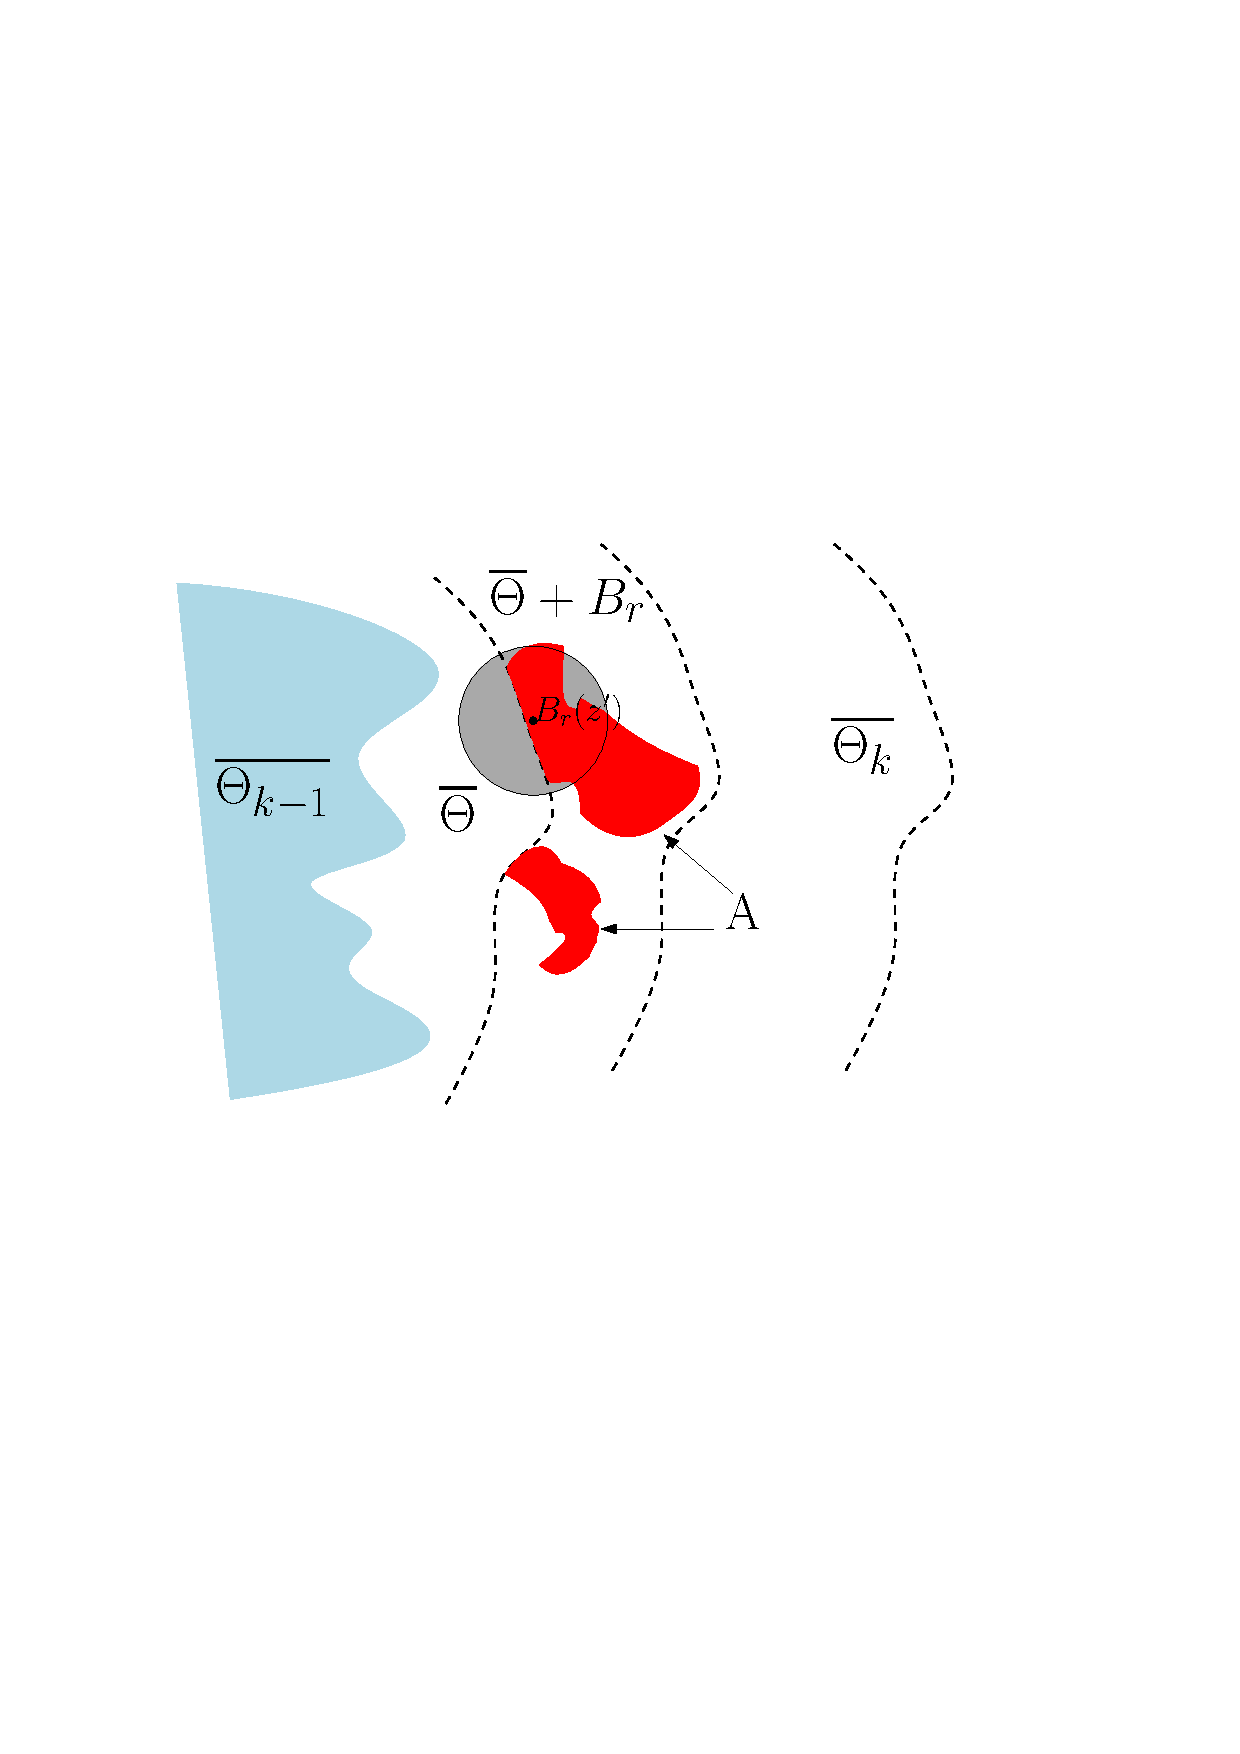
\includegraphics[width=0.5\textwidth]{Figures/div-sandpile-iteration.pdf}
		\caption{Illustration of the objects appearing in Step 1 of the proof of Proposition \ref{prop:div-sandpile-upper-bound}.
			Part of the current cluster $\overline{\Theta_{k-1}}$ is shown in light blue
			and parts of the boundaries of the intermediate clusters $\overline{\Theta}$ and $\overline{\Theta} + B_r$, defined in \eqref{eq:parameter-choices}
			and the next cluster $\overline{\Theta_k}$ are outlined by dashed lines. The ball $B_r(z')$ is shown in light gray 
			and part of the set $A$, defined in \eqref{eq:parameter-choices}, is shown in red. } \label{fig:div-sandpile-upper-bound-step1}
	\end{figure}
	
	\begin{proof}[Proof of Proposition \ref{prop:div-sandpile-upper-bound}] 
		Let $\delta \in (0, \rho)$ be given. Truncate on the event that $t < \TT$ and let $\Lambda_t$ be the harmonic ball satisfying the conditions in Theorem \ref{theorem:harmonic-balls}. 
		Since $\Lambda_t$ is open and contains the origin, we have that there exists a random $\sigma(h)$-measurable $s_0 \in (0,1)$ so that $B_{s_0} \Subset \Lambda_t$.
		
		For this $s_0$,  let the parameters $\omega, s_1, s_2, \boldsymbol{\delta}$ be as in Lemma \ref{lemma:constant-order-lower-bound-div}. Let $\beta^-$ be as in Lemma \ref{lemma:volume-growth} and
		\begin{equation} \label{eq:s6}
		s_6 := s_1^{-1} \boldsymbol{c_0}^{-2 \beta^-} 4^{2 \beta^-} \times C
		\end{equation}
		where $C$ and $\boldsymbol{c_0}$ are the deterministic constants from Lemma \ref{lemma:mass-bound-odometer}. Let $\boldsymbol{\delta_0} = \boldsymbol{\delta_0}(\boldsymbol{\delta}, \rho, \gamma) < \boldsymbol{\delta}$ be such that $(\boldsymbol{\delta_0} s_6)^{1/2 \beta^-} \leq \boldsymbol \delta$, so that Lemma \ref{lemma:constant-order-lower-bound-div} holds with $r \in ( 10 {\eps}^{\omega}, (\boldsymbol{\delta_0} s_6)^{1/2 \beta^-})$.  
		At the end of the proof we state how small $\boldsymbol{\delta_0}$ must be so that the final cluster is contained in ${\VGeps}(B_{\rho})$. Fix $\delta_0 <
		\boldsymbol{\delta_0}$ and decrease $\boldsymbol{\delta_0}$ so that $2 \times C_1 \times \boldsymbol{\delta_0}^\beta < \delta$ for a random constant $C_1$ to be determined below. 
		
		By the uniform convergence of the scaled version $\overline u_t^{\eps}$ of $u_t^{{\eps}}$ away from the origin (Theorem \ref{theorem:convergence-divisible} and Lemma \ref{lemma:uniform-convergence-of-greens-function}) and the fact that $\Lambda_t$ a.s.\ contains a neighborhood of 0, on the event $\{t < \TT\}$, 
		\begin{equation} \label{eq:start-iteration}
		\sup_{{\VGeps}(\partial \Lambda_t)} u_t^{{\eps}} < \delta_0 {\eps}^{-1},
		\end{equation}
		except on an event of probability tending to 0 as ${\eps} \to 0$.
		% CORRECTION [C8]: the printed proof did not impose the lower scale required by Lemma 7.2.
		Decrease $\omega$ if necessary so that $\omega < \beta$, where $\beta$ is from Lemma \ref{lemma:mass-bound-odometer}. Fix $\omega_0 \in (0,\omega)$ which we will choose in \eqref{eq:choice-of-omega0-div} below. Set
		$\Theta_0 = {\VGeps}(\Lambda_t)$, $r_0 = \delta_0$, $O_0 = \max_{\partial \Theta_0} u^{{\eps}}_t$
		and for $k \geq 1$, inductively define 
		\begin{equation} \label{eq:div-sandpile-cluster-iteration}
		\begin{cases}
		\mbox{Current cluster: } & \Theta_k := {\VGeps}(\overline{\Theta_{k-1}} + B_{r_{k-1}}) \\
		\mbox{Current radius: } & r_k :=  \max\left( (|O_{k-1}| \times {\eps} \times s_6)^{1/{2 \beta^-}}, 40 \boldsymbol{c_0}^{-1} {\eps}^{\omega_0} \right) \\
		\mbox{Current maximum odometer: } & O_k := \max_{\partial \Theta_k} u^{{\eps}}_t.
		\end{cases}
		\end{equation}
		Denote the first time the odometer is smaller than 
		${\eps}^{-\omega_0}$ by 
		\begin{equation} \label{eq:iterate-stop-time2-div}
		\tau_{{\eps},2} = \min\{ k \geq 0 : |O_k| \leq {\eps}^{-\omega_0} \}
		\end{equation}
		and the first time (before $\tau_{{\eps},2}$) that the current radius is less than $40 \boldsymbol{c_0}^{-1} {\eps}^{\omega_0}$ by 
		\begin{equation}
		\tau_{{\eps},1} = \min \left( \min\{ k \geq 0 : r_k \leq 40 \boldsymbol{c_0}^{-1} {\eps}^{\omega_0} \}, \tau_{{\eps},2} \right).
		\end{equation}
		By Lemma \ref{lemma:cell-size-estimate}, for each $\zeta > 0$, 
		\begin{equation} \label{eq:cell-size-estimate-local-div}
		\diam(H^{{\eps}}_a) \leq {\eps}^{2/(2+\gamma)^2 - \zeta} \quad \forall a \in {\VGeps}(B_{\rho}),
		\end{equation}
		w.p.\ tending to 1 as ${\eps} \to 0$. 
		Choose $\zeta$ in a way which depends only on $\gamma$ and then choose $\omega_0$ small enough so that 
		\begin{equation} \label{eq:choice-of-omega0-div}
		{\eps}_0^{-\omega_0}  \times {\eps}_0^{2/(2+\gamma)^2 - \zeta} \leq {\eps}_0^{\omega_0/2} ,\quad \forall {\eps}_0 \in (0,1) .
		\end{equation}
		
		
		{\it Step 1: $k < \tau_{{\eps},1}$.} \\
		We first show that for each $t \in \{1, \ldots, \tau_{{\eps},1}-1\}$,
		\begin{equation} \label{eq:iterative-bound-of-o}
		O_k \leq (1-s_2) O_{k-1},
		\end{equation}
		except on an event of probability tending to 0 as ${\eps} \to 0$.
		By Lemma \ref{lemma:mass-bound-odometer}, for all $z \in \C$ and $s \geq \eps^{\beta}$ such that $B_{s}(z) \subset B_{\rho} \setminus \overline{\Theta_{k-1}}$:
		\begin{equation} \label{eq:mass-bound-in-proof}
		\left| {\VGeps}(B_{\boldsymbol c_0 s}(z)) \cap \Lambdateps \right| \leq C \times \sup_{\partial \Theta_{k-1}} u_{t}^{{\eps}},
		\end{equation}
		where $\boldsymbol{c_0}$ is as in Lemma \ref{lemma:mass-bound-odometer}, except on an event of probability tending to 0 as ${\eps} \to 0$.
		As we justify just below, this implies we can apply Lemma \ref{lemma:constant-order-lower-bound-div} with parameters
		\begin{equation} \label{eq:parameter-choices}
		\begin{aligned}
		r &= \boldsymbol{c_0} r_k/4 \\
		\Theta &= {\VGeps}(\overline{\Theta_{k-1}} + B_{r_k/4}) \\
		A &= \Lambdateps \cap \{ {\VGeps}(\overline{\Theta} + B_r) \setminus \Theta \}.
		\end{aligned}
		\end{equation}
		See Figure \ref{fig:div-sandpile-upper-bound-step1} for an illustration of these sets. Indeed, we have that $A \subset {\VGeps}(\overline{\Theta} + B_r) \setminus \Theta$ and, by \eqref{eq:mass-bound-in-proof}, for $z \in \C$:
		\begin{align*}
		|A \cap {\VGeps}(B_r(z))|  &=
		|A \cap {\VGeps}(B_{\boldsymbol{c_0} r_k/4}(z))|  \\
		&\leq |\Lambdateps \cap {\VGeps}(B_{\boldsymbol{c_0} r_k/4}(z'))|  \\
		&\quad \mbox{(for some $z' \in \C$ s.t.\ $B_{r_k/4}(z') \subset B_{\rho} \setminus \overline{\Theta_{k-1}}$  by definition of $A$ \eqref{eq:parameter-choices})} \\
		&\leq C \times \sup_{\partial \Theta_{k-1}} u_t^{{\eps}} \quad \mbox{(by \eqref{eq:mass-bound-in-proof})} \\
		&= C \times O_{k-1}   \quad \mbox{(definition of $O_{k-1}$ \eqref{eq:div-sandpile-cluster-iteration})} \\
		&=  r_k^{2 \beta^-} \times {\eps}^{-1} \times s_6^{-1} \times C  \quad \mbox{(definition of $r_k$ \eqref{eq:div-sandpile-cluster-iteration})} \\
		&=  s_1  r^{2 \beta^-} {\eps}^{-1} \quad \mbox{(definition of $r$ and $s_6$  \eqref{eq:parameter-choices} and \eqref{eq:s6})}.
		\end{align*}
		Thus, as $r \geq 10 {\eps}^{\omega}$ the hypotheses of Lemma \ref{lemma:constant-order-lower-bound-div} are satisfied and we may apply it to get 
		\begin{equation} \label{eq:probability-bound-in-proof}
		\begin{aligned}
		\sup_{a \in {\VGeps}(\partial (\overline{\Theta_{k-1}} + B_{r_k/4 + \boldsymbol{c_0} r_k/8}))}
		\P[&\mbox{$X^{a, {\eps}}$ exits ${\VGeps}(\overline{\Theta_{k-1}} + B_{r_k/4 + \boldsymbol{c_0} r_k/4} )\setminus
			{\VGeps}(\overline{\Theta_{k-1}} + B_{r_k/4}))$} \\
		&\mbox{before exiting $A$} | h , \eta]  
		\leq (1 - s_2)
		\end{aligned}
		\end{equation}
		except on an event of probability tending to 0 as ${\eps} \to 0$.
		Next, by Lemma \ref{lemma:odometer-bound-mass} applied to the set 
		\[
		B := {\VGeps}(\overline{\Theta_{k-1}} + B_{r_k/4 + \boldsymbol{c_0} r_k/4} )\setminus
		{\VGeps}(\overline{\Theta_{k-1}} + B_{r_k/4})
		\]
		together with the maximum principle for $u_t^{{\eps}}$ ($u_t^{{\eps}} = 0$ on ${\VGeps}(\partial B_{\rho})$),
		\[
		u_t^{{\eps}}(b) \leq O_{k-1} \times \P[\mbox{$X^{b, {\eps}}$ exits $B$ before exiting $A$} | h , \eta], \quad \forall b \in B.
		\]
		Another application of the maximum principle shows 
		\[
		O_{k} \leq  \sup_{b \in {\VGeps}(\partial (\overline{\Theta_{k-1}} + B_{r_k/4 + \boldsymbol{c_0} r_k/8}))} u_{t}^{{\eps}}(b).
		\]
		The previous two indented equations together with \eqref{eq:probability-bound-in-proof} imply \eqref{eq:iterative-bound-of-o}.
		
		We now use \eqref{eq:iterative-bound-of-o}, the definition of $r_k$,  and the initial bound given by \eqref{eq:start-iteration} to see that
		\begin{equation} \label{eq:good-event3} 
		r_k \leq (\delta_0\times (1-s_2)^k \times s_6)^{1/2\beta^-}, \quad \forall k \in \{1, \ldots, \tau_{{\eps},1}-1\} 
		\end{equation} 
		and consequently, 
		\begin{equation} \label{eq:bound-on-radii-sum-div}
		\sum_{k=0}^{\tau_{{\eps},1}-1} r_k \leq \sum_{k=0}^{\tau_{{\eps},1}-1} (\delta_0\times (1-s_2)^k \times s_6)^{1/2\beta^-} \leq C \times \delta_0^{1/2\beta^-} \times \frac{1}{1 - (1-s_2)^{1/2\beta^-}},
		\end{equation}
		except on an event of probability tending to 0 as ${\eps} \to 0$ where $C = C(s_6) > 0$ is a random constant. 
		\medskip
		
		
		{\it Step 2: $t \in [\tau_{{\eps},1}, \tau_{{\eps},2})$.} \\
		We again apply Lemma \ref{lemma:constant-order-lower-bound-div} for each $k \in \{\tau_{{\eps},1}, \ldots, \tau_{{\eps},2}\}$ with the same choice of parameters as in Step 1.
		Reasoning similar to the proof of Step 1 shows that 
		\[
		O_k \leq (1-s_2) O_{k-1}, \quad \forall k \in \{\tau_{{\eps},1}, \ldots, \tau_{{\eps},2} \} 
		\]
		except on an event of probability tending to 0 as ${\eps} \to 0$.
		Hence, by the definition~\eqref{eq:iterate-stop-time2-div} of $\tau_{{\eps},2}$, 
		\[
		{\eps}^{-\omega_0} \leq |O_{\tau_{{\eps},2}-1}| \leq C (1-s_2)^{\tau_{{\eps},2}- \tau_{{\eps},1}-1} {\eps}^{-1}, \quad \mbox{for $C = C(s_6) > 0$} 
		\]
		which, upon re-arranging, implies
		\begin{equation} \label{eq:time-upper-bound-div}
		\tau_{{\eps},2} \leq C \log {\eps}^{-1} + \tau_{{\eps},1}, \quad \mbox{for random $C = C(s_2, s_6) > 0$} 
		\end{equation}
		and hence 
		\begin{equation}
		\sum_{k=\tau_{{\eps},1}}^{\tau_{{\eps},2}} r_k \leq C \times {\eps}^{\omega_0} \times \log {\eps}^{-1}, \quad \mbox{for random $C = C(s_2, s_6) > 0$}
		\end{equation}
		except on an event of probability tending to 0 as ${\eps} \to 0$.
		\medskip
		
		{\it Step 3: $k \geq \tau_{{\eps},2}$.} \\
		We control the size of the odometer by Lemma \ref{lemma:crude-upper-bound}
		and the upper bound on the Euclidean diameter of cells in the mated-CRT map. 
		By Lemma \ref{lemma:crude-upper-bound},  w.p.\ tending to 1 as ${\eps} \to 0$, for every $a \in \Lambdateps \setminus \Theta_{\tau_{{\eps},2}}$, there is a path
		of at most $\log({\eps}^{-1})^2 {\eps}^{-\omega_0}$ cells from $a$
		to $\partial \Theta_{\tau_{{\eps},2}}$ along which the odometer increases by at most ${\eps}^{-\omega_0}$.
		Thus, by the definition of $\tau_{{\eps},2}$, \eqref{eq:cell-size-estimate-local-div}, and \eqref{eq:choice-of-omega0-div}
		\begin{equation} \label{eq:distance-of-final-cluster-div-sandpile}
		u_t^{{\eps}}(a) = 0  \quad \mbox{for $a \in {\VGeps}(B_{\rho})$ such that $\dist(\eta(a), \eta(\Theta_{\tau_{{\eps},2}})) \geq  {\eps}^{\omega_0/2} \log({\eps}^{-1})^2$}
		\end{equation}
		except on an event of probability tending to 0 as ${\eps} \to 0$.
		\medskip
		
		{\it Step 4: Reduce ${\eps}$ and $\boldsymbol{\delta_0}$ and conclude.} \\
		Recall that we have set $\Theta_0 = {\VGeps}(\Lambda_t)$, so that $\overline\Theta_0$ is the union of the ${\eps}$-mated-CRT map cells which intersect $\Lambda_t$.
		By combining Steps 1-3, \eqref{eq:cluster-contained-in}, and \eqref{eq:consistency},
		the divisible sandpile cluster, $\overline{D}_{{\eps}}(t {\eps}^{-1})$ is contained in $\overline{\Theta_0} + B_R$, where
		\[
		\begin{aligned}
		R &=  C_1 \times \delta_0^{1/2\beta^-}  \quad \mbox{(by \eqref{eq:bound-on-radii-sum-div})} \\
		&+  C_1 \times {\eps}^{\omega} \times \log {\eps}^{-1}  \quad \mbox{(by \eqref{eq:time-upper-bound-div})} \\
		&+ {\eps}^{\omega_0/2} \log({\eps}^{-1})^2 \quad \mbox{(by \eqref{eq:distance-of-final-cluster-div-sandpile})} 
		\end{aligned}
		\]
		for random constants $C_1 = C_1(s_2, s_6, \beta^-, \gamma)$, provided that $R < \rho/2$,
		except on an event of probability tending to 0 as ${\eps} \to 0$.
		The first term in the definition of $R$ dominates for small ${\eps}$.
		Decrease $\boldsymbol{\delta_0}$ in a deterministic fashion and then decrease ${\eps}$ depending on $\delta_0$ so that $R < \rho/2$ and hence $u_t^{{\eps}} = v_t^{{\eps}}$.  
		This completes the proof after recalling that $\delta > 2 \times C_1 \boldsymbol{\delta_0}^\beta$. 
	\end{proof}
	
	\section{Convergence} \label{sec:proof-of-convergence}
	We start by combining Propositions \ref{prop:IDLA-lower-bound}, \ref{prop:IDLA-upper-bound}, \ref{prop:div-sandpile-lower-bound}, and  \ref{prop:div-sandpile-upper-bound}
	into the following statement. 
	\begin{prop} \label{prop:IDLA-constrained-convergence}
		Recall the time $\TT$ from~\eqref{eq:cluster-stopping-time}
		and the notation $B_{\delta}^{\pm}$ from \eqref{eq:outer-inner-neighborhoods}.  For each $\delta \in (0, \rho)$ and $t > 0$, on the event $\{t < \TT\}$, 
		it holds except on an event of probability tending to 0 as ${\eps} \to 0$  that
		\[
		\Bdeltam(\Lambda_t) \subset \overline{\mathcal{X}}_{{\eps}}(t {\eps}^{-1}) \subset \Bdeltap(\Lambda_t)
		\]
		for $\mathcal{X} \in \{A, D\}$,
		where $\Lambda_t$ is as in Theorem \ref{theorem:harmonic-balls},  \ie, both the IDLA cluster and divisible sandpile cluster converge. 
	\end{prop}
	To prove Theorems \ref{theorem:convergence-of-IDLA} and \ref{theorem:convergence-of-div-sandpile}, we will combine the previous proposition with a scaling argument to transfer from $t\in (0,\TT)$ to an arbitrary $t>0$.
	
	\subsection{Proof of Theorems \ref{theorem:convergence-of-IDLA} and \ref{theorem:convergence-of-div-sandpile}} \label{subsec:proof-of-idla}
	We use the scale-invariance property of the $\gamma$-quantum cone. Fix $b > 0$ and for $R_b$ as in 
	\eqref{eq:cone-scale-radius}, let
	\[
	h^b := h(R_b \cdot) + Q \log R_b - \frac{1}{\gamma} \log b \quad \text{and} \quad  \eta^b = R^{-1}_b \eta(b \cdot). 
	\]
	By Lemma \ref{lemma:scale-invariance}, $(h, \{\Lambda_t\}_{t > 0} ) \overset{d}{=} (h^b, \{ R_b^{-1} \Lambda_{b t} \}_{t>0})$.
	Hence, by the scale-invariance of the law of $\eta$, viewed modulo time parametrization, and the independence of $\eta$ and $(h, \{\Lambda_t\}_{t>0})$,
	\begin{equation} \label{eq:scale-invariance-of-field-and-eta}
	(h,\eta,\{\Lambda_t\}_{t > 0})  \overset{d}{=} (h^b,\eta^b , \{R_b^{-1} \Lambda_{b t}\}_{t > 0} ) .
	\end{equation}
	Hence, if we let
	\[
	T^b := \sup \{ t > 0 : R_b^{-1} \Lambda_{b t} \subset B_{\rho/3} \}
	\]
	then $T^b$ has the same law as $\TT$, defined in \eqref{eq:cluster-stopping-time}.
	By Proposition \ref{prop:IDLA-constrained-convergence}, for each $\delta \in (0, \rho)$ and $t > 0$, on the event $\{t < \TT\}$, 
	it holds except on an event of probability tending to 0 as ${\eps} \to 0$  that
	\[
	\Bdeltam(\Lambda_t) \subset \overline{\mathcal{X}}_{{\eps}}( t {\eps}^{-1} ) \subset \Bdeltap(\Lambda_t),
	\]
	for $\mathcal{X} \in \{A, D\}$, \ie, both the IDLA cluster and divisible sandpile cluster converge. 
	Let $\mathcal{X} \in \{A, D\}$ be given. 
	By \eqref{eq:scale-invariance-of-field-and-eta}, 
	this implies that for each $\delta \in (0, \rho)$ and $t > 0$, on the event $\{t < T^b\}$, 
	it holds except on an event of probability tending to 0 as ${\eps} \to 0$  that
	\[
	\Bdeltam(R^{-1}_b \Lambda_{b t}) \subset  R^{-1}_b \overline{\mathcal{X}}_{{\eps}}( b t {\eps}^{-1} ) \subset \Bdeltap(R^{-1}_b \Lambda_{b t}).
	\]
	By applying the above statement with $t/b$ in place of $t$ and $\delta / R_b$ in place of $\delta$, then re-scaling space by $R_b$, we get the following.
	For each $\delta \in (0, \rho)$ and $t > 0$, on the event $\{t < b \times T^b\}$, 
	it holds except on an event of probability tending to 0 as ${\eps} \to 0$  that
	\[
	\Bdeltam(\Lambda_t) \subset \overline{\mathcal{X}}_{{\eps}}( t {\eps}^{-1} ) \subset \Bdeltap(\Lambda_t).
	\]
	As $b > 0$ was arbitrary, it remains to show that in probability, 
	\begin{equation} \label{eq:btb-converge-to-inf}
	\lim_{b \to \infty} b \times T^b = \infty.
	\end{equation}
	This, however, follows immediately from the fact that $\TT$ is strictly positive and $\TT \overset{d}{=} T^b$.
	%for each $p \in (0,1)$, there exists $c_p > 0$ so that 
	%\[
	%\P[T^b > c_p] \geq p, \quad \forall b >0 .
	%\]
	%Hence,
	%\[
	%\P[ \cap_{m=1}^{\infty} \cup_{b = m}^{\infty} T^b > c_p] \geq p.
	%\]
	%Combining the previous two indented equations shows that with probability at least $p$,  $b \times T^b \to \infty$.
	%Since this holds for all $p \in (0,1)$, we have that the convergence of \eqref{eq:btb-converge-to-inf} occurs in probability. 
	\qed
	
		
	
	
	\appendix	
	\section{Discrete obstacle problem} \label{sec:obstacle-appendix}
We provide the proofs which were omitted in Section \ref{subsec:basic-properties} in the general setting of an undirected, locally finite, connected, and infinite graph $G$. We consider a finite set of vertices of $G$, denoted by $V$, which contain a marked vertex which we call the {\it origin}, denoted by $0$.  
	% CORRECTION [C33]: the hypotheses are weakened on V and strengthened on G (E-c1-2); connectedness of V is not used.
	\begin{remark}
	Connectedness of $V$ is not needed. Since $G$ is connected and infinite, every vertex of the finite set $V$ has a path in $G$ to $V^c$. Hence the finite maximum principle holds on every connected component of $V$, and the zero-boundary Dirichlet problem on $V$ has a unique solution: the homogeneous problem vanishes by the maximum principle applied to both signs, and existence follows from invertibility of the finite matrix. On a component of $V$ not containing $0$ the obstacle is harmonic and vanishes on the exterior boundary, hence vanishes; so the least supersolution vanishes there. The perturbation argument for $\Delta w=\mathfrak r$ on $\{w>\phi\}$ and $\Delta w\geq 0$ on $V$ is componentwise, and the exclusion of a component of $\{w>\phi\}$ away from $0$ uses the finite maximum principle on that component; hence the cluster is connected when nonempty. The upper and lower bounds and the mass identities sum over all of $V$ and do not use connectedness of $V$.
	\end{remark}
The graph Laplacian, $\Delta$, is defined by,
\[
\Delta u(a) =  \frac{1}{\deg(a)} \sum_{b \sim a}(u(b) - u(a)), \quad \mbox{for all vertices $a$ of $G$}
\]
where the sum $b \sim a$ is over the vertices $b$ which share an edge with $a$ and $\deg(a)$ denotes the number of such vertices.  Observe that the analogue of the maximum principle, Lemma \ref{lemma:maximum-principle}, and the following discrete divergence theorem are satisfied on $G$.


\begin{lemma} \label{lemma:discrete-divergence-theorem}
	Let $VG$ denote all the vertices of $G$ and suppose that $f,g: VG \to \R$ are functions which are zero outside of a finite subset of $VG$. 
	Then
	\begin{equation} \label{eq:gauss-green}
	\sum_{a \in VG} f(a) \Delta g(a) \deg(a) = \sum_{a \in VG} g(a) \Delta f(a) \deg(a).
	\end{equation}
\end{lemma}
\begin{proof}
	This is well known for general, undirected graphs --- see for example~\cite[Equation (2.17)]{telcs2006} or~\cite[Lemma 3.6]{berestycki2020random}.
\end{proof}

%\begin{proof}
%    Write $e_{x,y}$ for the indicator function that there is an edge between sites $x, y \in {\VGeps}$. 
%	We have, after unpacking the definitions and using compact support:
%	\begin{align*}
%	\sum_{x \in {\VGeps}} f(x) \Delta g(x) \deg^{{\eps}}(x) &= \sum_{x \in {\VGeps}} f(x) \sum_{y \in {\VGeps}} (g(y) - g(x)) e_{x,y}  \\
%	&= \sum_{x \in {\VGeps}} \sum_{y \in V} f(\textcolor{red}{x}) g(\textcolor{blue}{y}) e_{x,y}  -  \sum_{x \in {\VGeps}} \sum_{y \in {\VGeps}} f(x) g(x) e_{x,y} \\
%	&= \sum_{x \in {\VGeps}} \sum_{y \in V} f(\textcolor{blue}{y}) g(\textcolor{red}{x}) e_{x,y}  -  \sum_{x \in {\VGeps}} \sum_{y \in {\VGeps}} f(x) g(x) e_{x,y}  \qquad \mbox{($e_{x,y} = e_{y,x}$)} \\
%	&= \sum_{x \in {\VGeps}} g(x) \Delta^{{\eps}} f(x) \deg^{{\eps}}(x),
%	\end{align*}
%	completing the proof. 
%\end{proof}


Let $\mathfrak{r}:V \to (0, \infty)$ denote a {\it threshold function} 
and $\phi : \cl(V) \to (-\infty, 0]$ the {\it obstacle}
which satisfies the following equation
\begin{equation} \label{eq:laplacian-of-phi}
\begin{cases}
\Delta \phi  = \mathfrak t \delta_0 \quad \mbox{on $V$} \\
\phi = 0 \quad \mbox{on $\partial V$}
\end{cases}
\end{equation}
where $\mathfrak t > 0$. Consider the following {\it discrete obstacle problem}
\begin{equation} \label{eq:discrete-least-supersolution-general}
\begin{aligned}
w := &\min \{ u: \cl(V) \to \R : \Delta u \leq \mathfrak{r} \mbox{ on $V$ and $u \geq \phi$}\}.
\end{aligned}
\end{equation}
We will make use of the following function $\mathfrak{q}: \cl(V) \to \R$ which is defined by the unique solution to
\begin{equation} \label{eq:definition-of-exit-time-general}
\begin{cases}
\Delta \mathfrak q  = \mathfrak{r} \quad \mbox{on $V$} \\
\mathfrak{q} = 0 \quad \mbox{on $\partial V$}.
\end{cases}
\end{equation}
We also denote the {\it discrete cluster} by 
\begin{equation} \label{eq:discrete-cluster-general}
\Lambda = \{ a \in \cl(V) :  w(a) > \phi(a) \}.
\end{equation}



The results of Section \ref{subsec:basic-properties} may be achieved from those of this section 
via the following map, for ${\eps} > 0$, $\rho \in (0,1)$, 
\begin{align*}
\mathfrak{t} &\to {\eps}^{-1} t \deg^{{\eps}}(0)^{-1} \\
w &\to \wteps \\
G &\to {\Geps} \\
V &\to {\VGeps}(B_{\rho}) \setminus {\VGeps}(\partial B_{\rho}) \\
\mathfrak{r} &\to (\deg^{{\eps}})^{-1} \\
\phi &\to -(t {\eps}^{-1}) \times  \gr{{\eps}}{B_\rho}(0, \cdot) \\
\mathfrak q &\to  -\qeps{B_{\rho}} \\
\Lambda &\to \Lambdateps.
\end{align*}
Lemma \ref{lemma:discrete-basic-properties} is a special case of the following. 
\begin{lemma} \label{lemma:discrete-basic-properties-general}
	We have that
	\[
	\max(\mathfrak q,\phi) \leq w \leq 0
	\]
	and  $\Delta w \leq \mathfrak{r}$ on $V$.
\end{lemma}
\begin{proof}
	{\it Step 1: $w \leq 0$.} \\ 
	As $0 \geq \phi$ and $\mathfrak{r} > 0$ the function which is identically 0 is admissible in \eqref{eq:discrete-least-supersolution-general}.
	\medskip
	
	{\it Step 2: $w \geq \phi$ and $\Delta w \leq \mathfrak{r}$.} \\ 
	Observe that in general, for two functions $u_1, u_2$ defined on the vertices
	of the graph $G$, we have
	\[
	\Delta \min(u_1, u_2) \leq \min(\Delta u_1 , \Delta u_2),
	\]
	where the minimum is pointwise. 
	Indeed, write $u = \min(u_1,u_2)$ and suppose for a vertex $a$ that $u(a) = u_1(a)$. Then, by definition, 
	\[
	\Delta u(a) = \frac{1}{\deg(a)} \sum_{b \sim a}(u(b) - u_1(a))
	\leq \frac{1}{\deg(a)} \sum_{b \sim a}( u_1(b) - u_1(a)) = \Delta u_1(b). 
	\]
	Therefore, by compactness, the inequalities in the definition of \eqref{eq:discrete-least-supersolution-general}
	are also satisfied by $w$. 
	\medskip
	
	{\it Step 3: $w \geq \mathfrak q$.} \\ 
	By Steps 1 and 2, since $\phi$ is zero on $\partial V$, we have that $w$ is zero on $\partial V$. 
	Thus, by \eqref{eq:definition-of-exit-time-general} and Step 2, 	$(w - \mathfrak{q})$ is superharmonic on $V$ and zero on 
	$\partial V$, and hence the claim follows by the maximum principle.
\end{proof}

Lemma \ref{lemma:discrete-laplacian-bound} is a special case of the following. 
\begin{lemma} \label{lemma:discrete-laplacian-bound-general}
	We have that $\Delta w = \mathfrak{r}$ on $\Lambda$ 
	and $\mathfrak{r} \geq \Delta w \geq 0$ on $V$. 
	Moreover,  $\Lambda$ is connected and if $\mathfrak{t} > \mathfrak{r}(0)$, contains the origin. 
\end{lemma}
\begin{proof}
	{\it Step 1: $\Delta w = \mathfrak{r}$ on $\Lambda$.} \\
	Note that the inequality $\Delta w \leq \mathfrak{r}$ was established in Lemma \ref{lemma:discrete-basic-properties-general}. 
	Suppose for sake of contradiction $w > \phi$
	but $\Delta w(a) < \mathfrak{r}(a)$ for some $a \in V$.  Let 
	\[
	\delta = \min \left( \mathfrak{r}(a) - \Delta w(a), w(a) - \phi(a)  \right) > 0
	\]
	and consider the function $u: V \to \R$ defined by, 
	\[
	u := w - \delta \times 1\{ \cdot = a\}.
	\]
	We will see that the function $u$ is admissible in \eqref{eq:discrete-least-supersolution-general}, but strictly less than $w$,  a contradiction. 
	By definition 
	\[
	\Delta u(b) \leq \Delta w(b) \quad \forall b \neq a 
	\]
	and
	\begin{align*}
	\Delta u(a) &= \frac{1}{\deg(a)} \sum_{b \sim a} (w(b) - u(a))  
	=  \Delta w(a) + \delta 
	\leq \mathfrak{r}(a).
	\end{align*}
	Similarly, 
	\[
	u(b) = w(b) \geq \phi(b) \quad \forall b \neq a 
	\]
	and
	\begin{align*}
	u(a)  
	= w(a) - \delta  
	\geq  w(a) - w(a) + \phi(a) 
	=\phi(a), 
	\end{align*}
	completing the proof. 
	\medskip
	
	{\it Step 2: $\Delta w \geq 0$.} \\
	If $a \in V \cap \Lambda^c$, we have
	\begin{align*}
	\Delta w(a) &= \frac{1}{\deg(a)} \sum_{b \sim a} (w(b) -  w(a)) \\
	&= \frac{1}{\deg(a)} \sum_{b \sim a} (w(b) - \phi(a)) \quad \mbox{(assumption on $a$)} \\
	&\geq \Delta \phi(a)  \quad \mbox{(Lemma \ref{lemma:discrete-basic-properties-general})} \\
	&\geq 0 \quad \mbox{(since $\phi$ is subharmonic)}.
	\end{align*}
	In light of Step 1, this completes the proof. 
	\medskip
	
	{\it Step 3:  $\Lambda$ is connected.} \\
	Consider the function $v =  w - \phi$. 
	If $\Lambda$ is disconnected then there is a connected component of $\Lambda$ not containing the origin;
	call this component $A$. 
	By Step 1 and \eqref{eq:laplacian-of-phi}, we have that 
	\[
	\begin{cases}
	\Delta v = \mathfrak{r} \quad \mbox{on $A$} \\
	v > 0 \quad \mbox{on $A$} \\
	v = 0 \quad \mbox{on $\partial A$}, 
	\end{cases}
	\]
	which contradicts the maximum principle. 
	\medskip
	
	{\it Step 4: If $t > \mathfrak{r}(0)$,  $\Lambda$ contains the origin.} \\
	We demonstrate the contrapositive. Observe that the argument in Step 3 shows that $\Lambda$ is either empty or contains the origin. 
	If $\Lambda$ is empty, then
	\begin{align*}
	\mathfrak{t} &= \Delta \phi(0) \qquad \mbox{(by \eqref{eq:laplacian-of-phi})} \\
	&= 	\Delta  w(0) \qquad \mbox{(as $\Lambda$ is empty)} \\
	&\leq \mathfrak{r}(0) \qquad \mbox{(by Lemma \ref{lemma:discrete-basic-properties-general})},
	\end{align*}
	completing the proof. 
\end{proof}
We conclude with a discrete conservation of mass lemma; this is a general version
of Lemma \ref{lemma:discrete-conservation-of-mass}.
\begin{lemma} \label{lemma:discrete-conservation-of-mass-general}
	If $\mathfrak{r} = \deg^{-1}$, we have that $|\Lambda| \leq  \mathfrak{t} \times \deg(0)$. Moreover, 
	if $\Lambda \subset \inte(V)$,
	then  
	\[
	\sum_{a \in V} \Delta w(a) \deg(a) =  \mathfrak{t} \times \deg(0).
	\] 
\end{lemma}
\begin{proof}
	Let	$v = w - \phi$ and extend $v$ to a function on $VG$, the set of all vertices of $G$, by defining it to be zero on $\cl(V)^c$. 
	We compute, 
	\begin{align*}
	-\mathfrak{t} \times  \deg(0) + |\Lambda| &\leq \sum_{a \in V} \Delta v(a) \deg(a)
	\quad \mbox{(by Lemma \ref{lemma:discrete-laplacian-bound-general}, \eqref{eq:laplacian-of-phi}, and $\mathfrak{r} = \deg^{-1}$)} \\
	&= \sum_{a \in VG} 1\{ a \in V\}  \Delta v(a) \deg(a) \\
	&= \sum_{a \in VG}   v(a) \deg(a) \Delta 1\{ a \in V\} 
	\quad \mbox{(by Lemma \ref{lemma:discrete-divergence-theorem})} \\
	&= \sum_{a \in V}   v(a) \deg(a) \Delta 1\{ a \in V\} 
	\quad \mbox{($v = 0$ on $V^c$)} \\
	&= -\sum_{a \in V}  v(a)  \left( \mbox{\# neighbors of $a$ not in $V$} \right) \\
	&\leq 0 \quad \mbox{(since $v \geq 0$ by Lemma \ref{lemma:discrete-basic-properties-general})}.
	\end{align*}
	If $\Lambda \subset \inte(V)$, then $v = 0$ on all vertices which share an edge with a vertex in $\partial V$. 
	Thus, an identical computation, where the first line is replaced by 
	\[
	-\mathfrak{t} \times  \deg(0) + \sum_{a \in V} \Delta w(a) \deg(a) = \sum_{a \in V} \Delta v(a) \deg(a)
	\]
	and the last inequality by an equality, shows the moreover clause. 
\end{proof}

	
% CORRECTION [C16]: the occupation argument for Lemma 3.4 is transcribed in full in Appendix B; the printed proof is replaced by it.
\section{Occupation identity for the clock in Lemma 3.4}\label{app:occupation-proof}
For the circle-average clock of a $\gamma$-quantum cone we prove the killed occupation identity at each deterministic starting point, including the logarithmic singularity $0$, for all $\gamma\in(0,2)$. The coefficient is $2$ for unscaled Liouville Brownian motion and $\kappa_0=2/m_0$ for the time-rescaled process $X$ of Section~\ref{subsec:lbm-and-rw}. We also give a precise killed-process version of the argument in Lemma~\ref{lemma:integral-convergence-of-greens-function}.

\subsection{Statement, normalization, and exact inputs}

Write $B_a=B_a(0)$. Fix $\gamma\in(0,2)$, $\rho\in(0,1)$,
a deterministic disk $D=B_r(z)\subset B_\rho$, and a deterministic
$y\in D$. In particular, $\cl(D)$ is a compact subset of $B_1$.
Let $h$ be the circle-average embedding of a $\gamma$-quantum cone.
We use exactly the field and area normalization of the paper:
\begin{equation}\label{eq:field}
 h|_{B_1}\overset d=(g-\gamma\log|\cdot|)|_{B_1},
 \qquad
 \E[g(x)g(w)]=\log\frac1{|x-w|}\quad(x,w\in B_1),
\end{equation}
where $g$ is the whole-plane GFF with $g_1(0)=0$, and
$\mu_h=\lim_{\varepsilon\to0}\varepsilon^{\gamma^2/2}e^{\gamma h_\varepsilon(x)}\,dx$.
The first identity is equation \eqref{eq:gff} of the paper
and follows directly from its definition of the cone. In arguments
inside $B_1$ we couple the two sides of \eqref{eq:field}.

Conditionally on $\mathcal F=\sigma(h,\eta)$, sample standard planar Brownian
motion $B^y$, independently of this environment. Its generator is
$\tfrac12\Delta$. Put
\begin{equation}\label{eq:clock}
 \sigma=\inf\{s\geq0:B^y_s\notin D\},\qquad
 \phi_\varepsilon(s)=\int_0^{s\wedge\sigma}
       \varepsilon^{\gamma^2/2}e^{\gamma h_\varepsilon(B^y_u)}\,du .
\end{equation}
Here and below the continuum Dirichlet Green function has normalization
$\Delta G_D(y,\cdot)=-\delta_y$. In a disk, if
$a=(y-z)/r$ and $b=(x-z)/r$, it is
\begin{equation}\label{eq:green}
 G_D(y,x)=\frac1{2\pi}
     \log\left|\frac{1-\overline a b}{a-b}\right|.
\end{equation}
Consequently the ordinary Brownian occupation kernel is $2G_D$.
For example, this follows by applying It\^o's formula to the
zero-boundary solution of $-\tfrac12\Delta u=f$, first for smooth $f$,
and then by approximation and monotone convergence.

\begin{theorem}\label{thm:main}
The clocks in \eqref{eq:clock} converge, uniformly in $s\geq0$ in joint
probability over the field and Brownian motion, to a clock $\phi$.
Almost surely in the environment, $\phi$ is Brownian-almost surely
continuous, starts at $0$, is strictly increasing before $\sigma$,
and has $0<\phi(\sigma)<\infty$.

Define the unscaled process $Y_t^y=B^y_{\phi^{-1}(t)}$ before its exit
time $\tau_D^Y=\phi(\sigma)$, and the process of the paper by
$X_t^y=Y^y_{m_0t}$, with $\tau_D^X=\phi(\sigma)/m_0$.
Here $m_0$ is the unique deterministic annealed median of the raw exit time
of $Y^0$ from $B_{1/2}$, so $0<m_0<\infty$.
Almost surely in the environment, simultaneously for every bounded
Borel function $f:D\to\R$,
\begin{align}
 \E\left[\int_0^{\tau_D^Y}f(Y_t^y)\,dt\,\middle|\,h,\eta\right]
   &=2\int_DG_D(y,x)f(x)\,\mu_h(dx), \label{eq:raw}\\
 \E\left[\int_0^{\tau_D^X}f(X_t^y)\,dt\,\middle|\,h,\eta\right]
   &=\frac2{m_0}\int_DG_D(y,x)f(x)\,\mu_h(dx).
       \label{eq:scaled}
\end{align}
Both lifetimes have finite quenched mean. The event in this statement
may depend on the fixed parameters $\gamma,\rho,D,y$; it does not
depend on $f$. In particular the conclusion applies to every bounded
H\"older function which is measurable with respect to $(h,\eta)$.
\end{theorem}

\begin{remark}[What is, and is not, an approximation claim]\label{rem:mode}
The paper's display defining $\phi$ does not specify a mode of
convergence. Theorem~\ref{thm:main} constructs its precise
circle-average approximants in the full-$\varepsilon$ probability sense.
Every almost sure version of that displayed limit has the same value;
an almost surely convergent deterministic subsequence also exists.
We do not claim almost sure convergence along every real
$\varepsilon\downarrow0$ at the singular start. This precision does not change
the resulting clock or its quenched occupation identity.
\end{remark}

For clarity, the exact non-elementary inputs to the proof are listed
here. Page numbers refer to the versions specified in the bibliography.
\begin{enumerate}[label=(\roman*)]
\item Berestycki \cite[Theorem 1.1, p.~3; hypotheses (1.2)--(1.5),
pp.~2--3]{berestycki2017elementary}: for covariance
$\log|x-w|^{-1}$ plus a continuous function, and a finite reference
measure of finite $(d-\delta)$-energy for every $\delta>0$, the
variance-normalized GMC approximants converge in $L^1$ and probability
when $\gamma<\sqrt{2d}$, and weakly in probability as measures.
The uniform circle mollifier is explicitly admissible on p.~3.
\item Berestycki \cite[Theorem 1.2, p.~949, and its proof, p.~959;
Remark 3.5, p.~959]{berestycki2015diffusion}: the circle-average construction for a
zero-boundary GFF converges along dyadic scales and its pre-exit clock
is continuous and strictly increasing. Strict increase is proved in
the paragraph immediately preceding Remark 3.5; that remark proves
the absence of clock jumps. We use these precise clock conclusions.
\item Berestycki--Gwynne \cite[Lemma A.1, p.~66, equation (A.1)]{berestycki2020random}:
for the circle-average $\gamma$-cone and any small $\zeta>0$, with
polynomially high probability as $\delta\downarrow0$,
\begin{equation}\label{eq:BGmass}
 \delta^{(2+\gamma)^2/2+\zeta}
 \leq\mu_h(B_\delta(v))
 \leq\delta^{(2-\gamma)^2/2-\zeta},
 \qquad v\in B_{1-\delta}.
\end{equation}
\end{enumerate}
The additional exact inputs used only for Lemma 3.4 are recorded in
Section~\ref{sec:use}. In particular we do not use the assertion of the
singular-start Green formula in \cite[footnote 2, p.~9]{berestycki2020random} as a proof
of that formula.

\subsection{The nonsingular circle-average clock}

Let
\[
 \nu_\varepsilon(dx)=\varepsilon^{\gamma^2/2}e^{\gamma g_\varepsilon(x)}\,dx,
 \qquad \nu=\mu_g,\qquad
 A_\varepsilon(s)=\int_0^{s\wedge\sigma}
                \varepsilon^{\gamma^2/2}e^{\gamma g_\varepsilon(B^y_u)}\,du.
\]
For sufficiently small $\varepsilon$, all averaging circles centered in
$\cl(D)$ lie in $B_1$. Averaging the logarithmic covariance twice gives
\begin{equation}\label{eq:var}
 \operatorname{Var}(g_\varepsilon(x))=\log(1/\varepsilon),\qquad
 \E\nu_\varepsilon(dx)=dx.
\end{equation}
Thus there is no missing conformal-radius multiplier in this
normalization.

\begin{lemma}\label{lem:base}
The clocks $A_\varepsilon$ converge uniformly in $s\geq0$ in probability to a
continuous clock $A$, strictly increasing before $\sigma$.
For this specified deterministic $y$, on one event of full field
probability,
\begin{equation}\label{eq:base}
 \E_y\left[\int_0^\sigma q(B^y_s)\,dA(s)\,\middle|\,g\right]
       =2\int_DG_D(y,x)q(x)\,\nu(dx)
\end{equation}
simultaneously for every bounded Borel $q$.
\end{lemma}

\begin{proof}
First verify the hypothesis needed to apply \cite[Theorem 1.1,
p.~3]{berestycki2017elementary} conditionally on a Brownian path. For $0<a<2$ and an
integer $n$, Brownian Gaussian increments give
\[
 \E_y\int_0^n\int_0^n |B^y_s-B^y_t|^{-a}\,ds\,dt
   =C_a\int_0^n\int_0^n |s-t|^{-a/2}\,ds\,dt<\infty.
\]
Intersecting over integers $n$ and a countable sequence of exponents
tending to $2$, and using $\sigma<\infty$ almost surely, proves that
the Brownian occupation measure
$\lambda_B(E)=\int_0^\sigma\ones_{\{B^y_s\in E\}}\,ds$
has finite $a$-energy for every $a<2$. Its support is in $\cl(D)$,
strictly inside a larger disk in $B_1$.

For this reference measure, the theorem and \eqref{eq:var} give
convergence of $A_\varepsilon(\sigma)$ in $L^1$ in the field, conditionally
on almost every Brownian path. The same applies with $\sigma$ replaced
by $t\wedge\sigma$ and with bounded nonnegative continuous spatial
weights. Each conditional $L^1$ error is bounded by twice the reference
mass, because the approximants and limit have that mass as their
field expectation. Since
$\E_y\sigma=(r^2-|y-z|^2)/2<\infty$, dominated convergence over Brownian
paths gives joint $L^1$ convergence. Signed bounded weights follow by
splitting positive and negative parts.

Here is an explicit transfer of clock regularity from the precise
Dirichlet-field statement in \cite[Theorem 1.2, p.~949, proof and
Remark 3.5, p.~959]{berestycki2015diffusion}. Choose $\rho<R<1$. On $B_R$, the
logarithmic covariance is the sum of the zero-boundary disk GFF
covariance
\[
 \log\frac{R|1-x\overline w/R^2|}{|x-w|}
\]
and the covariance
\[
 K_H(x,w)=-\log R-\log|1-x\overline w/R^2|
   =-\log R+
       \operatorname{Re}\sum_{n\geq1}\frac{(x\overline w/R^2)^n}{n}.
\]
The latter is positive definite: it is the covariance of an independent
real Gaussian constant of variance $-\log R$ plus a harmonic Gaussian
power series. The series converges locally uniformly almost surely.
Thus $g$ has the law of $g^{\,0}+H$ there, with independent
zero-boundary GFF $g^{\,0}$ and harmonic continuous $H$.
On $\cl(D)$, $H$ is bounded and its sufficiently small circle averages
equal $H$. The clocks are therefore related by the continuous positive
multiplier $e^{\gamma H(B^y_s)}$. The cited Dirichlet clock is continuous
and strictly increasing, and its dyadic limit agrees with the
probability limit just obtained. This constructs $A$ with those
properties. Convergence at finitely many time points, monotonicity of
$A_\varepsilon$, and continuity of $A$ imply uniform convergence in probability
on each bounded time interval. Finally $\P_y(\sigma>n)\to0$ gives the
asserted uniform convergence on $s\geq0$.

For $q\in C(\cl(D))$, the ordinary Brownian Green identity gives
\begin{equation}\label{eq:baseapprox}
 \E_y\left[\int_0^\sigma q(B^y_s)\,dA_\varepsilon(s)\,\middle|\,g\right]
   =2\int_DG_D(y,x)q(x)\,\nu_\varepsilon(dx).
\end{equation}
The weighted clocks on the left converge in joint $L^1$ by the preceding
conditional-GMC argument. Their probability limit is the Stieltjes
integral against $A$, by its continuity and uniform clock convergence.
Conditional expectation is an $L^1$ contraction.

The right side of \eqref{eq:baseapprox} converges in $L^1$ in the field.
Indeed, first replace $G_D(y,\cdot)$ by its minimum with $M$ and apply
\cite[Theorem 1.1, p.~3]{berestycki2017elementary} with a bounded weighted Lebesgue
reference measure. The expected error, for both $\nu_\varepsilon$ and $\nu$,
is at most
\[
 2\|q\|_\infty
       \int_{\{G_D(y,x)>M\}}G_D(y,x)\,dx\longrightarrow0.
\]
Here $\E\nu(dx)=dx$ follows from the same $L^1$ theorem; the logarithmic
singularity is Lebesgue integrable. This proves \eqref{eq:base}
for each fixed continuous $q$.

Take a countable uniformly dense collection in $C(\cl(D))$ containing
$1$, for example the rational polynomials in the two coordinates.
On one field event, both sides define finite Borel measures on
$\cl(D)$ with identical integrals against this collection. Their
integrals agree for all continuous functions by uniform approximation,
so the measures agree. Both give zero mass to $\partial D$:
$A$ has no terminal atom and $G_D$ vanishes there.
Equality of the measures proves the assertion for every bounded Borel
$q$. This construction fixed $y$ at the outset and therefore has no
exceptional starting-point issue.
\end{proof}

\subsection{The logarithmic insertion and its actual regularization}

Choose a buffered radius $\rho<\rho_1<1$ and any
$b\in(0,(2-\gamma)^2/2)$. Apply \eqref{eq:BGmass} at dyadic radii and
use Borel--Cantelli and monotonicity. Almost surely there are finite
random constants $C$ and $r_0>0$ such that
\begin{equation}\label{eq:mass}
 \mu_h(B_a(v))\leq C a^b,\qquad
 v\in B_{\rho_1},\quad 0<a<r_0.
\end{equation}
On this event $\mu_h(\{0\})=0$. Off $0$, the circle average of
$-\log|\cdot|$ is $-\log|x|$ for $\varepsilon<|x|$. Local convergence of
the area measures on compact subsets away from $0$, followed by a
countable exhaustion, therefore gives
\begin{equation}\label{eq:weight}
 \mu_h(dx)=|x|^{-\gamma^2}\nu(dx)\quad\hbox{on }B_1.
\end{equation}
The value of the weight at $0$ is immaterial: $\nu(\{0\})=0$ follows
from $\E\nu(dx)=dx$, and $\mu_h(\{0\})=0$ was just proved.

Since \eqref{eq:green} implies
$2G_D(v,x)\leq C_D(1+\log^+(1/|v-x|))$, a dyadic annulus sum using
\eqref{eq:mass} gives
\begin{equation}\label{eq:potential}
 \sup_{v\in D}\int_DG_D(v,x)\,\mu_h(dx)<\infty .
\end{equation}
For the small-distance contribution the summable upper bound is a
constant times $\sum_{j\geq0}(j+1)2^{-jb}$; the remaining contribution
is bounded by local finiteness.

Using bounded truncations of $|x|^{-\gamma^2}$ in Lemma~\ref{lem:base},
define
\begin{equation}\label{eq:weightedclock}
 \Phi(s)=\int_0^{s\wedge\sigma}|B^y_u|^{-\gamma^2}\,dA(u).
\end{equation}
Monotone convergence and \eqref{eq:weight}--\eqref{eq:potential} give
\begin{equation}\label{eq:weightedmean}
 \E_y[\Phi(\sigma)\mid g]
       =2\int_DG_D(y,x)\,\mu_h(dx)<\infty .
\end{equation}
In particular $\Phi(\sigma)<\infty$ Brownian-almost surely.
Lemma~\ref{lem:base} with $q=\ones_{\{0\}}$ shows that
$dA$ gives no mass to $\{s:B^y_s=0\}$, even when $y=0$.
One may set the weight to any positive finite value at $0$.
The finite measure defining $d\Phi$ is absolutely continuous with
respect to the atomless measure $dA$. Thus $\Phi$ is continuous,
$\Phi(0)=0$, and it is strictly increasing before $\sigma$.
In particular there is no initial holding interval or clock atom at $0$.

It remains essential to identify \eqref{eq:weightedclock} with
\emph{the circle-average regularization in the paper}. Finite potentials
or a generic additive-functional correspondence alone would not do this.
We provide that identification next.

\begin{lemma}[Regularized origin tails]\label{lem:tails}
Put
\[
 \mu_\varepsilon(dx)=\varepsilon^{\gamma^2/2}e^{\gamma h_\varepsilon(x)}\,dx,\qquad
 0<p<\min\{1,4/\gamma^2-1\},\qquad
 \kappa=(2-\gamma^2/2)p-\gamma^2p^2/2>0 .
\]
For all sufficiently small $a,\varepsilon>0$, uniformly in $\varepsilon$,
\begin{equation}\label{eq:tail}
 \E\left[\left(\int_{B_a}
          (1+\log(1/|x|))\,\mu_\varepsilon(dx)\right)^p\right]
     \leq C a^\kappa(1+\log(1/a))^p .
\end{equation}
\end{lemma}

\begin{proof}
The circle mean-value formula, including at $x=0$, gives exactly
\begin{equation}\label{eq:regweight}
 \mu_\varepsilon(dx)=(|x|\vee\varepsilon)^{-\gamma^2}\nu_\varepsilon(dx).
\end{equation}
For $R<1$, the covariance in \eqref{eq:field} gives on $B_1$
\[
 g(Ru)=N_R+g^R(u),\qquad
 \operatorname{Var}(N_R)=\log(1/R),
\]
where $N_R=g_R(0)$ is independent of $g^R$ and
$g^R|_{B_1}\overset d=g|_{B_1}$.
For example $\operatorname{Cov}(g(Ru),g_R(0))=\log(1/R)$ for
$|u|<1$, and subtracting this covariance gives the claim.
Whenever the averaging circles lie in $B_R$, \eqref{eq:regweight}
therefore yields
\begin{equation}\label{eq:scale}
 \mu_\varepsilon(R\,du)
   =R^{2-\gamma^2/2}e^{\gamma N_R}
       (|u|\vee(\varepsilon/R))^{-\gamma^2}\nu^R_{\varepsilon/R}(du),
\end{equation}
where $\nu^R_\delta$ is the nonsingular regularization for $g^R$.
It has expectation $du$ on the sets used below, by \eqref{eq:var}.

First let $A_s=\{s/2<|x|\leq s\}$ and $\varepsilon\leq s/4$, and take
$R=2s$. In rescaled coordinates, $1/4<|u|\leq1/2$ and
$\varepsilon/R\leq1/8$. The insertion weight is bounded, while the
logarithmic factor is at most $C(1+\log(1/s))$.
Independence in \eqref{eq:scale}, followed by
$\E[V^p]\leq(\E V)^p$, gives
\[
 \E\left[\left(\int_{A_s}(1+\log(1/|x|))\,\mu_\varepsilon(dx)\right)^p\right]
  \leq C s^\kappa(1+\log(1/s))^p,
\]
since $\E e^{p\gamma N_R}=R^{-\gamma^2p^2/2}$.

For the regularization core $B_c$ with $c\leq4\varepsilon$, instead take
$R=8\varepsilon<1$. Then $\varepsilon/R=1/8$ and $c/R\leq1/2$.
The expected rescaled log-weighted integral is bounded by
$C(c/R)^2(1+\log(1/c))$, as follows by integrating the logarithm
against $du$; the insertion is bounded at this fixed rescaled
regularization. Thus
\[
 \E\left[\left(\int_{B_c}(1+\log(1/|x|))\,\mu_\varepsilon(dx)\right)^p\right]
 \leq C R^\kappa(c/R)^{2p}(1+\log(1/c))^p
 \leq C c^\kappa(1+\log(1/c))^p,
\]
where the last inequality uses $\kappa<2p$ and $c\leq R$.
This also covers $a\leq4\varepsilon$. Otherwise split $B_a$ into dyadic
annuli until the remaining core has radius at most $4\varepsilon$.
Use $(\sum_j v_j)^p\leq\sum_j v_j^p$ and
\[
 \sum_{j\geq0}(2^{-j}a)^\kappa
       (1+\log(1/a)+j\log2)^p
       \leq C a^\kappa(1+\log(1/a))^p
\]
to obtain \eqref{eq:tail}.
\end{proof}

\begin{proof}[Identification of the paper's clock]
Let $0\leq\chi_a\leq1$ be continuous, equal to $0$ on $B_a$ and $1$
off $B_{2a}$.
For $\varepsilon<a$, \eqref{eq:regweight} implies
\[
 \int_0^{s\wedge\sigma}\chi_a(B^y_u)
       \varepsilon^{\gamma^2/2}e^{\gamma h_\varepsilon(B^y_u)}\,du
   =\int_0^{s\wedge\sigma}
        \chi_a(B^y_u)|B^y_u|^{-\gamma^2}\,dA_\varepsilon(u).
\]
For fixed $a$ these integrals converge uniformly in $s$ in probability
to the corresponding integral against $A$. To justify this
Stieltjes continuity assertion directly, restrict first to
$\{\sigma\leq n\}$, approximate the continuous time function
$\chi_a(B^y_u)|B^y_u|^{-\gamma^2}$ uniformly by step functions,
and use uniform convergence of the integrators and their total masses.
Then let $n\to\infty$.

The removed nonnegative part is bounded, uniformly in $s$, by
\[
 R_{\varepsilon,a}=\int_0^\sigma\ones_{\{|B^y_u|<2a\}}
                  \varepsilon^{\gamma^2/2}e^{\gamma h_\varepsilon(B^y_u)}\,du.
\]
Ordinary Brownian occupation gives
\[
 U_{\varepsilon,a}(g):=\E_y[R_{\varepsilon,a}\mid g]
       =2\int_{D\cap B_{2a}}G_D(y,x)\,\mu_\varepsilon(dx).
\]
For $y=0$, $G_D(0,x)\leq C_D(1+\log(1/|x|))$ near $0$.
For $y\ne0$, the kernel is bounded there if $2a<|y|/2$.
Consequently Lemma~\ref{lem:tails} and conditional Markov inequality
give, for every $u>0$,
\begin{align*}
 \P(R_{\varepsilon,a}>u)
 &\leq\E\min\{1,U_{\varepsilon,a}/u\}\\
 &\leq u^{-p}\E[U_{\varepsilon,a}^p]
 \leq C_{D,y}u^{-p}a^\kappa(1+\log(1/a))^p\longrightarrow0 ,
\end{align*}
uniformly in sufficiently small $\varepsilon$. The removed part for $\Phi$
tends to zero almost surely: its total mass is finite by
\eqref{eq:weightedmean}, and the limiting set $\{B^y_u=0\}$ has
zero clock mass. First let $\varepsilon\to0$ with $a$ fixed, and then
$a\to0$. We conclude that
\[
 \sup_{s\geq0}|\phi_\varepsilon(s)-\Phi(s)|\longrightarrow0
       \quad\hbox{in probability}.
\]
This proves the required identification $\phi=\Phi$, including
at $y=0$, throughout $\gamma\in(0,2)$.
No annealed first moment of the inserted clock was used.
These constructions agree on nested disks up to the smaller Brownian
exit time: their stopped approximants are identical, so uniqueness
of the probability limit gives the same stopped clock. Thus this
identification also supplies the restriction of the paper's clock
when a larger ambient disk is used.
\end{proof}

\subsection{Occupation identity, simultaneity, and the coefficient}

\begin{proof}[Proof of Theorem~\ref{thm:main}]
The clock construction and its regularity have been proved above.
For a fixed environment, extend \eqref{eq:base} by monotone convergence
to nonnegative Borel functions. Equations \eqref{eq:weight} and
\eqref{eq:weightedclock} then identify, as finite Borel measures,
\[
 \E_y\left[\int_0^\sigma\ones_{\{B^y_s\in dx\}}\,d\phi(s)
                 \,\middle|\,g\right]
     =2G_D(y,x)\,\mu_h(dx).
\]
The equality holds on the same event as in Lemma~\ref{lem:base}
and \eqref{eq:potential}, simultaneously for all Borel sets.
In particular its integral against any bounded Borel $f$ is legitimate
and absolutely integrable.

A continuous strictly increasing clock maps $[0,\sigma]$ onto
$[0,\phi(\sigma)]$. The change of variables for its Stieltjes measure
therefore gives, pathwise,
\[
 \int_0^{\tau_D^Y}f(Y_t^y)\,dt
       =\int_0^\sigma f(B^y_s)\,d\phi(s).
\]
This proves \eqref{eq:raw}. Strict positivity and finiteness of the
raw exit time also show that its annealed median from $0$ in $B_{1/2}$
is deterministic, positive, and finite. To check uniqueness, take
$1/2<R<1$ in the Gaussian decomposition used in
\eqref{eq:scale}. The raw exit time $L$ has the representation
$L=e^{\gamma N_R}L'$, with $N_R$ a nondegenerate Gaussian independent
of $0<L'<\infty$. Hence $\log L$ has a strictly positive continuous
density, obtained by convolving the law of $\log L'$ with a Gaussian
density. Its median is unique. Finally $X_t=Y_{m_0t}$,
so changing variables $s=m_0t$ proves \eqref{eq:scaled}.

The argument is local in $h|_{B_1}$, so the law identity
\eqref{eq:field} transfers it to the cone. Conditional Brownian
sampling is independent of the entire pair $(h,\eta)$; all kernels
used above are functions of $h$ alone. Conditioning additionally on
$\eta$ therefore leaves them unchanged. The finite-measure identity
holds before choosing $f$, which proves the claimed simultaneity and
allows environment-measurable $f$. Complex-valued tests follow by
treating their real and imaginary parts separately.
\end{proof}

The assertion with coefficient $2$ for the process $X$ is
false, and not merely inconsistent notation.
For a concrete parameter choice take $\gamma=1/2$ and let
$L=\tau_{B_R}^{Y,0}$ with $R=1/2$. By \eqref{eq:weight},
$\E\nu(dx)=dx$, \eqref{eq:raw}, and Tonelli,
\[
 \E L
   =2\int_0^R s^{1-\gamma^2}\log(R/s)\,ds
   =\frac{2R^{2-\gamma^2}}{(2-\gamma^2)^2}<0.195 .
\]
Thus $\P(L\geq1)<1/2$, so every median $m_0$ is less than $1$.
For $f=1$, the positive Green integral in \eqref{eq:scaled} then
rules out coefficient $2$. The minimal coefficient correction is
$\kappa_0=2/m_0$, the constant defined after \eqref{eq:mo}.
Alternatively, coefficient $2$ is correct if the named process is
changed from $X$ to the raw process $Y$.

A remark on the median: equation
\eqref{eq:mo} must use the starting point $0$, i.e.
\[
 m_0=\operatorname{median}
       \left(\inf\{t\geq0:|Y_t^0|\geq1/2\}\right).
\]
It cannot define a different $m_0$ for each displayed $z$:
the discrete median in \eqref{eq:meps} is taken from $0$,
and a start outside $B_{1/2}$ would give median zero.

\subsection{The use in Lemma 3.4}\label{sec:use}

We use the paper with the constant $\kappa_0$ defined after \eqref{eq:mo}.
Its conclusion in Lemma~\ref{lemma:integral-convergence-of-greens-function} needs no change of coefficient or
quantifiers. Its proof should explicitly use killed occupation in
$D=B_r(z)$. A path frozen at its boundary point has infinite
occupation of $f=1$ over $[0,\infty)$; stopping only on leaving
$B_\rho$ does not give the Green function of $D$.

We now give the convergence-to-occupation step.
For the embedded walk, put
\[
 I_\varepsilon=\mathcal{VG}^\varepsilon(D)\setminus\mathcal{VG}^\varepsilon(\partial D),\qquad
 K_\varepsilon=\inf\{k\geq0:X_k^{y,\varepsilon}\notin I_\varepsilon\},\qquad
 W^\varepsilon(t)=\eta(X^{y,\varepsilon}_{m_\varepsilon t}),
\]
with linear interpolation in the last expression. Use full walks,
or walks observed until leaving a larger buffered disk.
Let $\tau=\tau_D^X$ for the accelerated continuum process.

The exact external inputs here are
\cite[Theorem 1.2, p.~10]{berestycki2020random}, giving quenched convergence in
probability in the topology of local uniform convergence of paths;
\cite[Remark 1.3, equation (1.8), p.~10]{berestycki2020random}, giving
$m_\varepsilon\asymp\varepsilon^{-1}$; \cite[Lemma 2.4, equation (2.8),
p.~17]{berestycki2020random}, giving vanishing maximal cell diameter on buffered
compact disks with polynomially high probability; and
\cite[Proposition 5.1, equation (5.1), p.~28]{berestycki2020random}, giving,
on an event of polynomially high probability, the bounds
\begin{equation}\label{eq:discretemom}
 \E[(\tau^\eps_U)^N\mid h,\eta]
 \leq N!C^N\varepsilon^{-N}
  \left(\sup_{v\in U}
       \int_{B_{\varepsilon^\alpha}(U)}
         \left(\log\frac1{|v-w|}+1\right)\mu_h(dw)\right)^N
\end{equation}
for all positive integers $N$ and admissible Borel
$U\subset B_{\rho_1}$ with $\mu_h(U)\geq\varepsilon^\alpha$.
Its $\tau_U^\varepsilon$ is exit from the cells intersecting $U$;
$K_\varepsilon$ kills no later, so it satisfies the same upper bound.

Start with any deterministic sequence $\varepsilon\downarrow0$.
Pass to a deterministic subsequence on
which the quenched path laws converge almost surely, the maximal
relevant cell diameter $d_\varepsilon$ tends to zero almost surely, and
\eqref{eq:discretemom} holds eventually. The mass condition for the
fixed disk holds eventually because $\mu_h(D)>0$ almost surely.
The logarithmic integral in \eqref{eq:discretemom} is bounded uniformly
on its tail by the same annulus argument as \eqref{eq:potential},
using the buffered radius and \eqref{eq:mass}. Taking $N=2$ yields
a finite random $M$ with
\begin{equation}\label{eq:UI}
 \E[(K_\varepsilon/m_\varepsilon)^2\mid h,\eta]\leq M,\qquad
 \E[(K_\varepsilon/m_\varepsilon-T)_+\mid h,\eta]\leq M/T .
\end{equation}

Fix an environment in this event and in the event of
Theorem~\ref{thm:main}, also applied in a buffered disk. Couple its
quenched path laws by the Skorokhod representation, so that
$W^\varepsilon\to X$ locally uniformly almost surely. Then
\begin{equation}\label{eq:exitconv}
 K_\varepsilon/m_\varepsilon\longrightarrow\tau
       \quad\hbox{almost surely under the coupling}.
\end{equation}
We give the pathwise detail since exit time is not continuous at
every continuous path. If $t<\tau$, the compact path $X([0,t])$
has positive distance from $D^c$. Uniform convergence and shrinking
cells imply that every visited cell before time $m_\varepsilon t$ lies
inside $D$ and misses $\partial D$. This proves the lower bound
in \eqref{eq:exitconv}.

At ordinary Brownian exit from a disk, the projection of subsequent
increments onto the outward normal is one-dimensional Brownian
motion by the strong Markov property. The reflection principle
shows it has positive values arbitrarily soon. Thus Brownian motion
visits the strict exterior of the closed disk arbitrarily soon after
exit. The continuous strictly increasing clock in the buffered disk
transfers these visits to $X$ at times arbitrarily close after
$\tau$. At any such time, the exterior point is at positive distance
from $\cl(D)$, and this persists under uniform convergence.
A linear segment with a point outside the convex closed disk has
an endpoint outside it; that endpoint's cell cannot belong to
$I_\varepsilon$. The corresponding mesh time differs by at most
$m_\varepsilon^{-1}\to0$. This proves the upper bound and hence
\eqref{eq:exitconv}.

Let $f$ be any bounded H\"older function on $D$, measurable with
respect to the environment. It has a unique continuous extension
to $\cl(D)$. Compose that extension with nearest-point projection
onto the closed disk to obtain a bounded H\"older extension
$\widetilde f$ to $\C$. After the environment is fixed this is
an ordinary fixed function, of some exponent $\theta>0$ and
constant $H<\infty$. The coupling gives, for each fixed $T$,
\[
 \int_0^{T\wedge(K_\varepsilon/m_\varepsilon)}
             \widetilde f(W^\varepsilon(t))\,dt
       \longrightarrow \int_0^{T\wedge\tau}f(X_t)\,dt .
\]
The bound $T\|f\|_\infty$ permits passage to quenched expectations.
Adjacent cells intersect, so the relevant interpolation segments
have length at most $2d_\varepsilon$. The difference from the discrete
Riemann sum over $0\leq k<K_\varepsilon$, $k<m_\varepsilon T$, divided by
$m_\varepsilon$, is at most
\[
 T H(2d_\varepsilon)^\theta+2\|f\|_\infty/m_\varepsilon .
\]
The time horizon is fixed here; a uniform error independent of all
$T>0$ is unnecessary.

By \eqref{eq:UI}, the expected discarded discrete tail is at most
$\|f\|_\infty(M/T+m_\varepsilon^{-1})$. The continuum tail tends to zero
because $\E[\tau\mid h,\eta]<\infty$ by
Theorem~\ref{thm:main}. Letting first $\varepsilon\to0$ and then $T\to\infty$
proves
\begin{align*}
 m_\varepsilon^{-1}\sum_{b\in I_\varepsilon}
       \operatorname{Gr}_{D}^{\varepsilon}(a_y^\varepsilon,b)f(\eta(b))
 &=m_\varepsilon^{-1}\E\left[\sum_{k<K_\varepsilon}
             f(\eta(X_k^{y,\varepsilon}))\,\middle|\,h,\eta\right]\\
 &\longrightarrow
   \E\left[\int_0^\tau f(X_t^y)\,dt\,\middle|\,h,\eta\right]\\
 &=\frac2{m_0}\int_DG_D(y,x)f(x)\,\mu_h(dx).
\end{align*}
The sum may equivalently range over all cells intersecting $D$
if one uses $\widetilde f$: their killed Green function is zero
outside $I_\varepsilon$. This avoids evaluating $f$ at a representative
outside its domain.

Every deterministic input sequence has a deterministic subsequence
with this almost sure conclusion. The subsequence criterion gives
convergence in probability along all meshes, as required in
Lemma 3.4. The fixed-environment argument works for all bounded
H\"older tests on the same event, so it also justifies the
environment-dependent tests in that lemma.


% CORRECTION [C13]: the replacement argument for Lemma 3.6 (continuous datum, nearest-point projection, uniform convergence) is transcribed in full in Appendix C.

\section{Replacement proof of Lemma 3.6}\label{app:lemma36}
Throughout, the notation is that of the paper. Fix $\gamma\in(0,2)$, $\rho<1$, and a
deterministic disk $D=B_r(z)\subset B_\rho(0)$.
Take $h$ to be the circle-average embedding of a
$\gamma$-quantum cone, and decorate it by an independent
whole-plane space-filling $\mathrm{SLE}_{16/\gamma^2}$,
subsequently parameterized by $\mu_h$-area and denoted by
$\eta$. Use the associated mated-CRT cell-adjacency graph,
with edge multiplicities counted in simple random walk.
Let $\mathcal F=\sigma(h,\eta)$ and let
$H^\eps_a=\eta([a-\varepsilon,a])$ be the cell of $a\in\varepsilon\mathbb Z$.
Adjacent cells intersect. The cells are connected and locally finite.
Set
\[
 I^\eps_D=\mathcal{VG}^{\varepsilon}(D)\setminus\mathcal{VG}^{\varepsilon}(\partial D),\qquad
 \sigma^\eps_D=\inf\{j\ge0:X^\eps_j\notin I^\eps_D\},
\]
where $X^\varepsilon$ is one \emph{unrestricted} simple random walk started
at $a_y^\varepsilon=\min\{a\in\varepsilon\mathbb Z:y\in H^\eps_a\}$,
and $\mathcal{VG}^{\varepsilon}(A)=\{a:H^\eps_a\cap A\ne\varnothing\}$.
Use this same walk for every stopping operation below.
Write $Y^\eps_j=\eta(X^\eps_j)$ and let $W^\varepsilon$ be its linearly
interpolated embedding, with any positive deterministic time
rescaling, for instance $m_\varepsilon$ from the paper.
Define
\[
 T_D(W)=\inf\{t\ge0:W(t)\notin D\},\qquad
 Z^\varepsilon=W^\varepsilon(T_D(W^\varepsilon)).
\]
For a path that starts outside $D$ we project its initial point onto
$\overline D$; this harmless convention is irrelevant eventually for
each fixed $y\in D$.

There are three distinct issues in the printed proof.
\begin{enumerate}[label=(\roman*)]
\item A boundary cell need not have its representative $\eta(a)$ in
$\overline D$. Therefore $\psi(\eta(X^\eps_{\sigma^\eps_D}))$ is
not defined if $\psi$ is specified only on $\overline D$.
\item The exit functional is not an everywhere-defined continuous
functional on the printed path space. A constant path in $D$ never
exits. Uniform convergence of paths need not preserve exit locations
at a path that touches the boundary and returns without crossing.
Moreover the interpolated paths in the proof live in the outer
domain, not necessarily in $\overline D$.
\item The walk denoted $\widehat X^{y,\varepsilon}$ there is stopped on
boundary \emph{cells} of $B_\rho$. In particular, for $D=B_\rho$
it can be frozen at a representative inside $D$, so its Euclidean
exit time can be infinite. Small cell size alone also does not
control the excursion after first visiting a boundary cell.
\end{enumerate}
The last display additionally mixes the notation for LBM and the
discrete walk. It must use $X^{y,\varepsilon}$ in both discrete expressions.

For an explicit discontinuity example, take $D=B_1(0)$ and a
real-valued continuous path which runs from $0$ to $1$ in time
$1$, returns to $0$ in the next unit of time, and then runs
at unit speed toward $-\infty$. Its first exit is at $1$.
Multiplying this path by $1-1/n$, $n\ge2$, gives paths converging
locally uniformly to it whose first exit is at $-1$.
For $\psi(w)=\operatorname{Re}w$ the exit functional therefore
does not converge. This is why its limiting-law continuity
set must be checked.

The minimal boundary-value convention is
\[
 \bar\psi=\psi\circ\pi_D,\qquad
 \pi_D:\C\longrightarrow\overline D
\]
the nearest-point projection onto the closed disk.
It is $1$-Lipschitz, so a $\chi$-H\"older constant of $\psi$ is also
one for $\bar\psi$. The minimal path convention for the proof is to
use the unrestricted interpolation $W^\varepsilon$. A precise convention
which also works for the printed outer-stopped interpolation is
given in Section~\ref{sec:outer}.

\begin{theorem}[Lemma 3.6 with continuous data]\label{thm:A}
For every deterministic $\psi\in C(\overline D)$ and $y\in D$,
\begin{equation}\label{eq:A-main}
 \E[\bar\psi(Y^\eps_{\sigma^\eps_D})\mid\mathcal F]
 \ \longrightarrow\
 \E[\psi(X^y_{\tau_D})\mid\mathcal F]
 =:u(y)
 \quad\hbox{in probability}.
\end{equation}
Here $X^y$ is the rescaled LBM in the paper. The function $u$ is
the deterministic classical harmonic extension of
$\psi|_{\partial D}$. In fact the cellwise discrete harmonic
extensions converge uniformly on $\overline D$, in probability.
For H\"older $\psi$ the same-walk comparison in
Theorem~\ref{thm:rate} below gives a polynomial rate.
\end{theorem}

\subsection{Precisely stated inputs}
All page numbers refer to the linked arXiv versions, not journal
pagination.
\begin{enumerate}[label=(\alph*)]
\item Berestycki--Gwynne, arXiv:2003.10320v2,
Theorem 1.2, p.~10: the conditional law of the unrestricted
interpolated embedded walk, with the paper's median time
normalization, converges in probability in the local uniform path
topology to rescaled LBM. The theorem is uniform over starting
points in a fixed compact set.
\item The same paper, Lemma 2.4, p.~17: for each fixed
$\rho_1<1$ and $0<a<2/(2+\gamma)^2$, with probability
$1-O(\varepsilon^\kappa)$, for some $\kappa>0$, every cell meeting
$B_{\rho_1}$ has diameter at most $\varepsilon^a$.
\item Gwynne--Miller--Sheffield, arXiv:1807.07511v3,
Lemma 3.11, (3.35), p.~31: there are
$\alpha_{\rm ann}=\alpha_{\rm ann}(\gamma)>0$,
$b_{\rm ann}=b_{\rm ann}(\gamma)>0$, and
$p=p(\rho_1,\gamma)>0$ such that, with probability
$1-O(\varepsilon^{\alpha_{\rm ann}})$, simultaneously for every
$c\in B_{\rho_1}$ and
$R\ge\varepsilon^{b_{\rm ann}}$ with $B_{2R}(c)\subset B_{\rho_1}$,
one has
\[
 \inf_{v\in\mathcal{VG}^{\varepsilon}(B_R(c))}
 \P_v[\mathcal D_R(c)\mid\mathcal F]\ge p.
\]
Here $\mathcal D_R(c)$ is the event that $X^\varepsilon$ disconnects
$\mathcal{VG}^{\varepsilon}(\partial B_{R/2}(c))$ from $\mathcal{VG}^{\varepsilon}(\partial B_{2R}(c))$
before hitting the latter set.
Disconnection here means separation in the planar graph by
the vertices visited by the walk. We decrease $p$ to be at
most $1/2$ when convenient.
\item The same paper, Lemma 3.10, (3.34), p.~31:
for random walk on a graph which almost surely hits a set $A$,
the total variation distance between its first-hit distributions
on $A$, started from $v$ and $w$, is at most
\[
 1-\P_v[X\text{ disconnects }w\text{ from }A
                      \text{ before hitting }A].
\]
We apply this on a finite graph, with extra edges between
stopping vertices if needed to make it connected. The
construction below checks the connectedness and almost-sure
hitting hypotheses explicitly.
\end{enumerate}
The argument below uses these annulus and coupling inputs directly;
it does not require an explicit boundary H\"older exponent.
In particular it avoids a mesh-scale absorption issue in
the proof of Theorem 3.9 of Gwynne--Miller--Sheffield,
p.~32, (3.37): uniformly in a boundary distance $u$,
a factor $((\varepsilon^{b_{\rm ann}}\vee s)/u)^c$ cannot in general
be bounded by $C((\varepsilon\vee s)/u)^{c'}$ merely by decreasing
$c'$. For example, if $0<b_{\rm ann}<1$, $u=\varepsilon^{b_{\rm ann}}$
and $s\le\varepsilon$, the first factor is $1$ and the second tends
to $0$. We therefore retain the mesoscopic cutoff and do not
extract numerical comparison exponents from (3.33).
This is consistent with the weaker formulation of Lemma~\ref{lemma:discrete-holder-continuity}.

\subsection{The quantitative boundary-excursion estimate}
Fix $\rho<\rho_1<1$ and any
$0<a<2/(2+\gamma)^2$, and set
\begin{equation}\label{eq:exponents}
 \begin{gathered}
 b=\min\{a,b_{\rm ann}\}>0,\qquad d=\varepsilon^a,\qquad
 \ell=100d+\varepsilon^{b_{\rm ann}},\\
 \varepsilon^b\le\ell\le101\varepsilon^b,\qquad
 \nu=\frac{-\log(1-p)}{\log2}>0.
 \end{gathered}
\end{equation}
Choosing $a$ as a function of $\gamma$ makes $b=b(\gamma)$,
whereas $\nu$ can depend on $\rho_1$.
Let $E_\varepsilon\in\mathcal F$ be the intersection of the cell-size event
in (b) with the simultaneous annulus event in (c). Then
\[
 \P(E_\varepsilon^c)\le C\varepsilon^\kappa
\]
for some $\kappa>0$. Notice that $\ell\ge\varepsilon^{b_{\rm ann}}$
and $d<\ell/100$. All annuli used below have radii at least
$\ell$; no estimate is applied below its permitted cutoff.
Only this fixed separation between the cell size and
the first annulus radius is needed.

We first make explicit the planar observation needed with (c).
Let $O$ be a disk, $x\in O$, $B_{3R}(x)\subset B_{\rho_1}$,
and suppose
\[
 R/2>\dist(x,\partial O)+20d.
\]
A walk all of whose visited cells are contained in $O$ cannot
disconnect $\mathcal{VG}^{\varepsilon}(\partial B_{R/2}(x))$ from
$\mathcal{VG}^{\varepsilon}(\partial B_{2R}(x))$.
Indeed take the outward radial segment about the center of
$O$ from $u\in\partial B_{R/2}(x)$ to
$w\in\partial B_{2R}(x)$. Its distance from $O$ is greater
than $20d$. Choose cells containing $u,w$; their vertices
belong to the respective circle vertex sets.
Use the usual planar cell-adjacency drawing, with vertices
in their cells and edges in arbitrarily small neighborhoods
of the unions of incident cells. Choose perturbations of
size less than $d/10$ to accommodate pinch points.
Join the two chosen embedded vertices to $u,w$, respectively,
and insert the radial segment between these short joins.
The resulting curve stays at distance greater than $18d$
from $O$.

Here is why following faces along this curve is legitimate
even when cells have nontrivial topology. In the buffered
region, every point is within $2d$ of an embedded vertex,
since some cell contains the point. Consequently a face
meeting the curve has boundary within $2d$ of it; otherwise
that nearby vertex would lie in the interior of the face.
An edge there belongs to neighborhoods of its incident cells.
These cells, and the third incident cell of the triangular
face, all meet the ambient cell-size region. Each has
diameter at most $d$. They intersect pairwise, so their
union has diameter at most $3d$; the face boundary, and
hence the bounded face itself, have diameter less than $4d$.
The latter assertion follows because a bounded face is
contained in the convex hull of its boundary.

Local finiteness now gives a finite chain of closed faces
along the curve, consecutive faces sharing an edge or a
vertex. Their boundary vertices give a graph path between
the two chosen vertices. Every cell on this path is within
$6d$ of the curve and is therefore disjoint from $O$.
Thus the path avoids every visited vertex, contradicting
graph disconnection. This also checks the endpoint
membership in the two prescribed circle vertex sets.
Equivalently this is the planar separation
observation in the proof of GMS Theorem 3.9, p.~32, immediately
before (3.38); the buffer here makes its application insensitive
to cell representatives. This auxiliary planar drawing is
used only for graph separation; $W^\varepsilon$ remains the
straight-line interpolation specified at the start.

\begin{lemma}[Excursion after a boundary-cell hit]\label{lem:excursion}
On $E_\varepsilon$, for all sufficiently small $\varepsilon$, uniformly
over walks started in $I_D^\varepsilon$,
\begin{equation}\label{eq:spatial-tail}
 \P\bigl[|Z^\varepsilon-Y^\eps_{\sigma_D^\varepsilon}|>C s\mid\mathcal F\bigr]
 \le \min\{1,C(\ell/s)^\nu\},\qquad 0<s\le s_0,
\end{equation}
where $s_0>0$ is deterministic. The same estimate bounds the
maximal displacement from $Y^\eps_{\sigma_D^\varepsilon}$ after that
visit and before Euclidean exit, if exit has not already
occurred on the entering edge.
\end{lemma}
\begin{proof}
An interior cell is contained in $D$, by connectedness.
The first noninterior cell reached from $I_D^\varepsilon$ meets
$\partial D$: it intersects its preceding interior cell and
cannot be wholly outside $D$. Its representative is therefore
within $d$ of $\partial D$.
Before the edge entering it, all interpolated segments lie in
the convex disk $D$. If Euclidean exit occurs on the entering
edge, its distance from the endpoint is at most $2d$, since
adjacent cell representatives have distance at most $2d$.

Otherwise let $v=X^\eps_{\sigma_D^\varepsilon}$,
$x=\eta(v)\in D$, and put $O=B_{r+3d}(z)$.
The cell of $v$ is contained in $O$, and
$\dist(x,\partial O)\le4d$.
A first visit to $\mathcal{VG}^{\varepsilon}(\partial O)$ has representative at
distance at least $r+2d$ from $z$.
Consequently the interpolation has exited $D$ by that visit.
It is enough to control the walk's excursion before hitting
$\mathcal{VG}^{\varepsilon}(\partial O)$.

Let $R_j=2^j\ell$, and retain indices with $2R_j\le s_0$,
where $s_0<(\rho_1-\rho)/2$ is small enough that even
$B_{3R_j}(x)\subset B_{\rho_1}$. At the initial stage
the walk is at $v$.
At each subsequent stage restart it at its first hit of
$\mathcal{VG}^{\varepsilon}(\partial B_{2R_{j-1}}(x))$, unless it has already hit
$\mathcal{VG}^{\varepsilon}(\partial O)$. The restart cell meets the open disk
$B_{R_j}(x)$ even though $2R_{j-1}=R_j$:
it intersects the preceding cell, which is contained
in $B_{R_j}(x)$ since this is the first boundary-cell hit.
Its representative need not lie in that open disk, but
input (c) requires exactly membership in $\mathcal{VG}^{\varepsilon}(B_{R_j}(x))$.
Also the restart cell cannot already meet
$\partial B_{2R_j}(x)$, since its diameter is at most
$d<R_j/100$. Thus consecutive dyadic radii give legitimate
successive stopping times.
For small $\varepsilon$ the planar observation applies at every
stage, because $R_j/2\ge\ell/2>50d$ whereas
$\dist(x,\partial O)+20d\le24d$.
Thus the disconnection event in input (c) forces a visit
to $\mathcal{VG}^{\varepsilon}(\partial O)$ before reaching
$\mathcal{VG}^{\varepsilon}(\partial B_{2R_j}(x))$.
The conditional chance of surviving to that outer circle
without visiting $\mathcal{VG}^{\varepsilon}(\partial O)$ is at most $1-p$.

The strong Markov property, applied successively to these
stopping times, now gives a survival probability at most
$(1-p)^{j+1}$ through stage $j$. The annuli overlap; no
independence is being used. The uniform conditional bound
$1-p$ at each restart is the only input to the product.
Before the first boundary-cell hit for $B_{2R_j}(x)$,
all representatives lie in $B_{2R_j}(x)$; the representative
of the hit cell lies in $B_{2R_j+d}(x)$. Convexity gives the
same bound for interpolated segments.
For a displacement scale $s\ge4\ell$, choose the largest $j$
with $2R_j\le s/2$. Since $R_j=2^j\ell$,
\[
 (1-p)^{j+1}\le C(\ell/s)^\nu.
\]
A displacement greater than a fixed multiple of $s$ before
Euclidean exit requires survival through this stage.
The cases $s<4\ell$ follow by enlarging the constant and using
the bound $1$. Conditional on the environment the annulus
event is uniform over all centers, radii, and starting
vertices, so it remains applicable to the random $x$.
Finally apply the strong Markov property at $\sigma_D^\varepsilon$.
\end{proof}

\begin{theorem}[Quantitative comparison]\label{thm:rate}
Suppose $\psi$ is $\chi$-H\"older on $\overline D$, with
$0<\chi\le1$ and H\"older constant $H$.
Fix $y\in D$ and start the walk at $a_y^\varepsilon$.
Define $\Phi^\psi(W)=\psi(W(T_D(W)))$ on paths which start
inside $D$ and exit in finite time, and set it equal to $0$
on all remaining paths. For every
\[
                         0<q<b\chi
\]
one may take $C_\psi=1+H$ so that, for small $\varepsilon$,
\begin{equation}\label{eq:rate}
 \P\!\left[
 |\Phi^\psi(W^\varepsilon)-\bar\psi(Y^\eps_{\sigma_D^\varepsilon})|
       >C_\psi\varepsilon^q\right]
 \le C\bigl(\varepsilon^\kappa+\varepsilon^{\nu(b-q/\chi)}\bigr).
\end{equation}
On $E_\varepsilon$ the corresponding conditional probability is at
most $C\varepsilon^{\nu(b-q/\chi)}$, uniformly over interior starting
vertices. Moreover, on $E_\varepsilon$,
\begin{equation}\label{eq:mean-rate}
 \E[|\Phi^\psi(W^\varepsilon)-\bar\psi(Y^\eps_{\sigma_D^\varepsilon})|
       \mid\mathcal F]\le
 \begin{cases}
 C H\varepsilon^{b\chi},&0<\chi<\nu,\\
 C H\varepsilon^{b\nu}(1+|\log\varepsilon|),&\chi=\nu,\\
 C H\varepsilon^{b\nu},&\nu<\chi\le1 .
 \end{cases}
\end{equation}
In particular, choosing $a=(2+\gamma)^{-2}$ permits
\[
 q=\frac{\chi}{2}\min\{(2+\gamma)^{-2},b_{\rm ann}(\gamma)\},
\]
with exactly the dependence requested in the printed comparison.
More generally, by choosing $a$ close enough to its upper
endpoint, every
\begin{equation}\label{eq:full-q-range}
 0<q<\chi\min\{2/(2+\gamma)^2,b_{\rm ann}(\gamma)\}
\end{equation}
is allowed.
\end{theorem}
\begin{proof}
For fixed $y\in D$, its starting cell is interior on $E_\varepsilon$
for all small $\varepsilon$.
The unrestricted walk exits the finite cell domain associated
with $B_{r+3d}(z)$ almost surely, so its interpolation exits $D$.
Projection is nonexpansive and fixes its exit point
$Z^\varepsilon\in\partial D$. Hence
\[
 |\psi(Z^\varepsilon)-\bar\psi(Y^\eps_{\sigma_D^\varepsilon})|
 \le H|Z^\varepsilon-Y^\eps_{\sigma_D^\varepsilon}|^\chi.
\]
Use Lemma~\ref{lem:excursion} with $Cs=\varepsilon^{q/\chi}$,
which is larger than a fixed multiple of $\ell$ for small
$\varepsilon$, and add $\P(E_\varepsilon^c)$.
For the mean, write $R=|Z^\varepsilon-Y^\eps_{\sigma_D^\varepsilon}|
\le2r+d$. By monotonicity the tail bound extends, with a
different constant, to $s\le2r+d$.
Split
\[
 \E[R^\chi\mid\mathcal F]
 =\chi\int_0^{2r+d}s^{\chi-1}\P[R>s\mid\mathcal F]\,ds
\]
at a constant multiple of $\ell$.
The remaining integral is bounded by
$C\ell^\nu\int_\ell^{2r+d}s^{\chi-\nu-1}\,ds$.
Its three elementary cases give \eqref{eq:mean-rate}.
\end{proof}
The ambient radius enters $\nu$, the probability exponent
$\kappa$, and multiplicative constants, but not the choice
$q=b(\gamma)\chi/2$ or $C_\psi=1+H$.
This is a rate comparing two stopping rules for the same walk.
It supplies neither a convergence rate to Brownian harmonic
measure nor an optimal numerical exponent.

\subsection{Continuity at the limiting paths and proof of the lemma}
\begin{lemma}[Exit-map continuity]\label{lem:exit-continuity}
Let $w$ start in $D$, let $\tau=T_D(w)<\infty$, and suppose that
for each $\delta>0$ some $t\in(\tau,\tau+\delta)$ has
$w(t)\notin\overline D$. At such a path the exit time and exit
location maps are continuous for local uniform convergence.
\end{lemma}
\begin{proof}
For each $s<\tau$, the compact set $w([0,s])$ lies at positive
distance from $D^c$, so all sufficiently close paths have exit
time greater than $s$. Choose $t\in(\tau,\tau+\delta)$ at positive
distance from $\overline D$; sufficiently close paths exit by $t$.
Thus their exit times converge to $\tau$. Uniform continuity of
$w$ on a compact time interval containing those times then proves
convergence of the exit locations.
\end{proof}

For Brownian motion the exit time from a disk is finite almost
surely. At its exit point $p$, projection of the subsequent Brownian
increments onto the outward unit normal is a one-dimensional
Brownian motion. The probability that this projection stays
nonpositive on any interval $(0,\delta)$ is zero (for example,
the reflection principle gives the distribution of its maximum).
The strong Markov property and a countable intersection over
rational $\delta>0$ imply the crossing hypothesis of
Lemma~\ref{lem:exit-continuity}. LBM is the same Brownian trace
under a continuous strictly increasing clock, finite up to exit
from bounded disks, so it has the same property.
These assertions hold for almost every environment under its
conditional LBM law, by disintegration. Time rescaling by $m_0$
does not change the exit location.

For the path-law argument choose the median clock $m_\varepsilon$
specified in input (a). All stopping locations and values
under consideration are unchanged by positive deterministic
time rescaling, so this choice does not restrict the result.
Now start with an arbitrary deterministic sequence
$\eps_j\to0$. By input (a), extract a deterministic subsequence
along which the conditional path laws converge almost surely.
For each environment in this event the bounded exit functional
is continuous almost everywhere under the limiting law.
The bounded almost-everywhere-continuous version of the
portmanteau theorem therefore gives
\[
 \E[\Phi^\psi(W^\varepsilon)\mid\mathcal F]
 \longrightarrow\E[\psi(X^y_{\tau_D})\mid\mathcal F]
 \quad\hbox{almost surely along that subsequence}.
\]
Here one may see the portmanteau implication directly by replacing a
bounded function by its upper and lower $\delta$-oscillation
envelopes: the envelopes converge to the function at continuity
points, and the upper and lower weak-convergence inequalities,
followed by bounded convergence, squeeze their integrals.
No assertion that the exit functional is continuous everywhere
has been used.

For H\"older $\psi$, \eqref{eq:mean-rate} and
$\P(E_\varepsilon^c)\to0$ show that replacing
$\Phi^\psi(W^\varepsilon)$ by $\bar\psi(Y^\eps_{\sigma_D^\varepsilon})$
changes its conditional expectation by a quantity tending to
zero in probability. The arbitrary-subsequence criterion now
proves \eqref{eq:A-main}. Equivalently, choose a further
deterministic subsequence with summable exceptional probabilities.

The LBM exit distribution is the Brownian exit distribution.
The latter has density
\[
 u(y)=\int_0^{2\pi}
 \psi(z+re^{it})\,
 \frac{r^2-|y-z|^2}{|re^{it}-(y-z)|^2}\,\frac{dt}{2\pi}.
\]
The Poisson kernel is harmonic in $y$, integrates to $1$, and
concentrates at the boundary point as $y$ tends to that point.
This proves harmonicity, continuity up to the boundary, and the
assertion that $u$ is deterministic.

We prove the uniform assertion directly, also keeping the
cutoff in the compactness argument.
Write $f^\varepsilon(v)=\E_v[\bar\psi(Y_{\sigma_D^\varepsilon})\mid\mathcal F]$,
so $\|f^\varepsilon\|_\infty\le\|\psi\|_\infty$.
Here is the finite graph to which input (d) is applied.
Keep $I_D^\varepsilon$ and the stopping vertices
$A=\mathcal{VG}^{\varepsilon}(\partial D)$, together with all original edges incident
to $I_D^\varepsilon$. Every neighbor of an interior vertex belongs
to $I_D^\varepsilon\cup A$, by connectedness of its cell.
Every component containing an interior vertex reaches $A$:
otherwise it would be a finite component of the connected
infinite mated-CRT graph.
Add edges between vertices of $A$ to connect the remaining
components if necessary. This finite graph is connected,
and its walk hits $A$ almost surely from every vertex.
The walk before that hit, its hitting distribution, and
the event of disconnecting a vertex from $A$ are unchanged
by the added edges. Thus all hypotheses of input (d) hold.
Fix a compact $K\Subset D$ and let
$\delta=\dist(K,\partial D)>0$.
For representatives $x=\eta(v)$ and $x'=\eta(w)$ near $K$,
start the annulus iteration at
\[
 R_0=8(\ell\vee|x-x'|)
\]
and use radii $2^jR_0$ until $2\cdot2^jR_0\le\delta/4$.
If $R_0$ is already larger than this bound the following
estimate is trivial after enlarging its constant.
Otherwise the cell of $w$ lies inside the innermost circle,
and every cell of $\partial D$ lies beyond the outermost
circle, for small $\varepsilon$. A disconnection at any stage
therefore separates $w$ from the stopping set
$\mathcal{VG}^{\varepsilon}(\partial D)$. The walk cannot hit that stopping set
before hitting the stage's outer circle.
The Markov iteration in Lemma~\ref{lem:excursion}, now counting
failure of all disconnection attempts, bounds its probability
by $C(R_0/\delta)^\nu$.
Input (d) and the expectation formula consequently give
\begin{equation}\label{eq:interior-modulus}
 |f^\varepsilon(v)-f^\varepsilon(w)|
 \le C\|\psi\|_\infty
       \left(\frac{\ell\vee|x-x'|}{\delta}\right)^\nu.
\end{equation}
All constants here are uniform in the vertices of the
chosen compact set.

For boundary control, take an interior representative $x$
at distance $u$ from $\partial D$ and start the same iteration
at $R_0=8(\ell+u)$, now stopping on $\mathcal{VG}^{\varepsilon}(\partial D)$ itself.
For $u$ small this gives
\[
 \P_x[|Y_{\sigma_D^\varepsilon}-x|>Cs\mid\mathcal F]
 \le \min\{1,C((\ell+u)/s)^\nu\},\qquad 0<s\le s_0.
\]
The proof is identical to Lemma~\ref{lem:excursion}:
the radial complement of $D$ forces a boundary hit on each
successful disconnection, and $R_0/2>u+20d$.
Let $p$ be the nearest point of $\partial D$ to $x$.
With
$\omega_\psi(t)=\sup\{|\psi(v)-\psi(w)|:
v,w\in\overline D,\ |v-w|\le t\}$,
nonexpansiveness of projection implies
\begin{equation}\label{eq:boundary-modulus}
 |f^\varepsilon(v)-\psi(p)|
 \le \omega_\psi(Cs+u)
       +C\|\psi\|_\infty((\ell+u)/s)^\nu .
\end{equation}
Choose $s=\sqrt{\ell+u}$ for small $\ell+u$.
The right side tends to zero uniformly as $\ell+u\to0$.
For a starting boundary cell the prescribed value differs
from the value at a boundary point in the cell by at most
$\omega_\psi(d)$, so the same limiting assertion holds.
This includes cells touching the boundary only from outside.

Now prepare, from any deterministic sequence of $\varepsilon$'s,
a deterministic subsequence on which convergence holds at a
countable dense set of points in $D$ and $E_\varepsilon$ holds
eventually almost surely. Diagonal selection with summable
error probabilities does this.
On a compact subset of $D$, \eqref{eq:interior-modulus} and
$|\eta(a_y^\varepsilon)-y|\le d$ give asymptotic equicontinuity of
the cellwise extensions. A finite net from the dense set
therefore upgrades their pointwise convergence to uniform
convergence on that compact subset.
Estimate \eqref{eq:boundary-modulus} controls the remaining
boundary strip, uniformly in $\varepsilon$, and the limiting
Poisson extension is uniformly continuous on $\overline D$.
First shrink the strip and then let $\varepsilon\to0$.
This proves almost-sure uniform convergence along the
prepared subsequence, hence uniform convergence in probability
by the arbitrary-subsequence criterion.

Finally approximate a continuous datum uniformly on
$\overline D$ by deterministic Lipschitz functions. Projection
preserves the uniform approximation, and both discrete and
continuum harmonic extension are contractions in the sup norm,
by their expectation formulas. The uniform conclusion and
\eqref{eq:A-main} follow for continuous $\psi$ as well.
This proves Theorem~\ref{thm:A}.

\subsection{The actual outer-stopped interpolation}\label{sec:outer}
Here is a precise repair if one wants to retain
$\widehat X^{y,\varepsilon}$ from the printed proof. For an eventually
constant path $w$ which starts in $D$, set
\[
 \Phi^\psi_{\rm stop}(w)=
 \begin{cases}
 \psi(w(T_D(w))),&T_D(w)<\infty,\\
 \bar\psi(w(\infty)),&T_D(w)=\infty.
 \end{cases}
\]
Use the projected initial value when the path starts outside $D$.
With this convention \eqref{eq:rate} and \eqref{eq:mean-rate}
hold with $\Phi^\psi_{\rm stop}(\widehat X^{y,\varepsilon})$ in place
of $\Phi^\psi(W^\varepsilon)$. Indeed $\sigma_D^\varepsilon\le
\sigma_{B_\rho}^\varepsilon$. If the outer-stopped path has not exited
$D$, its final point occurs during the excursion before the
unrestricted path's first exit. The maximal-excursion assertion
of Lemma~\ref{lem:excursion} bounds its displacement from
$Y^\eps_{\sigma_D^\varepsilon}$ by the same argument.
Projection can only decrease the relevant distance.

If $\overline D\subset B_\rho$, the outer-stopped path does exit
$D$ on the cell-size event for small $\varepsilon$, and this convention
agrees with the printed functional. Without such a separation,
one must supply a convention or use the unrestricted walk.
For the proof of harmonic convergence, the unrestricted walk
avoids any need to apply a continuity theorem to this extended
outer-stopped functional.

For any two fixed H\"older extensions of the same $\psi$, their
values at a boundary-cell representative differ by $O(d^\chi)$:
compare each to a point of $\partial D$ in that cell.
Thus the limiting lemma is independent of the chosen extension.
The defects above are defects of definition and proof; after
these repairs the polynomial comparison itself is valid.

\subsection{Uses of Lemma 3.6 in the paper}
The definition of Lemma~\ref{lemma:convergence-of-harmonic-functions} is followed by one invocation, in the proof of Lemma~\ref{lemma:discrete-dirichlet-problem}. Each use is checked below.
\begin{enumerate}[label=(\arabic*)]
\item \textbf{Discrete Dirichlet problem (Lemma~\ref{lemma:discrete-dirichlet-problem}).}
Its harmonic part satisfies, exactly,
\[
 m_\varepsilon^{-1}f_1^\varepsilon(a_y^\varepsilon)
 =\E[\bar\phi(Y^\varepsilon_{\sigma_D^\varepsilon})\mid\mathcal F].
\]
Theorem~\ref{thm:A} gives the required convergence at every fixed rational point. A deterministic diagonal subsequence gives the almost-sure simultaneous statement for all rational points. The uniform conclusion of Theorem~\ref{thm:A} supplies the harmonic-part compactness and the boundary convergence. The boundary datum in that lemma must also be extended to a neighbourhood of $\overline D$ (or evaluated after $\pi_D$). No convergence rate is used in this invocation.

The inhomogeneous part uses the separate occupation-convergence lemma, Lemma~\ref{lemma:integral-convergence-of-greens-function}. Its correct limit is $-\kappa_0\int_D G_D(\cdot,w)\psi(w)\,\mu_h(dw)$, where $\kappa_0=2/m_0$. The displayed residual $m_0$ in Step 1 of the same computation must be read as $\kappa_0$. Likewise the limit of $m_\varepsilon^{-1}\mathfrak Q_D^\varepsilon$ has Laplacian $-\kappa_0\mu_h$, not the displayed $-1$ in Step 3 of the corresponding computation. The needed zero-boundary control is supplied by the lens comparison in the tightness argument of Section~\ref{sec:dirichlet-problem}; one cannot justify it by a harmonic maximum principle for the superharmonic exit-time function alone. These corrections do not require a stronger version of Lemma~\ref{lemma:convergence-of-harmonic-functions}.

\item \textbf{Normalized exit time (Lemma~\ref{lemma:convergence-of-the-normalized-exit-time}).}
These uses apply Lemma~\ref{lemma:discrete-dirichlet-problem} only with zero boundary data and a countable family of deterministic smooth sources. The harmonic part is identically zero. Deterministic diagonal preparation as in Lemma~\ref{lemma:discrete-potential-tightness} suffices. There is no demand for uncountably many simultaneous applications, or for a rate.

\item \textbf{Odometer compactness (Subsection ``Convergence of the odometer along subsequences'').}
This cites the zero-boundary barrier of the proof of Lemma~\ref{lemma:discrete-dirichlet-problem}. Use the lens barrier identified in item (1). It is a bounded-Laplacian estimate, not an extra consequence of pointwise harmonic convergence.

\item \textbf{Subsequential properties (Lemma~\ref{lemma:subsequential-properties}).}
The prepared family consists of rational balls and rational polynomial boundary data, hence is countable. A polynomial chosen after observing the limiting odometer is permissible because convergence has already been prepared for every member of that countable family. Polynomials have canonical extensions outside the disk. In the proof, the boundary condition must be
\[
 f_\delta^\varepsilon(b)=m_\varepsilon\bigl(\phi^\delta(\eta(b))+\delta\bigr),
\]
not $m_\varepsilon\phi^\delta(\eta(b))+\delta$. The latter has limit $\phi^\delta$ and cannot imply the displayed limit $\phi^\delta+\delta$ or the claimed domination. With this boundary value, uniform convergence of the odometer and $\|\phi^\delta-\bar w_t^*\|_{\overline D}<\delta/4$ give boundary domination for small $\varepsilon$; the small overshoot outside $D$ is handled by continuity on its collar. The discrete maximum principle and Theorem~\ref{thm:A} then give the asserted harmonic comparison. It is enough to take rational $\delta\downarrow0$, keeping the family countable.
\end{enumerate}
The introduction and the sentence preceding Lemma~\ref{lemma:convergence-of-the-normalized-exit-time} only announce or discuss the Dirichlet result. There are no other invocations of Lemma~\ref{lemma:convergence-of-harmonic-functions}, and no downstream invocation uses its printed quantitative comparison. This list concerns the uses of harmonic convergence only; it does not cover other Green-kernel or obstacle calculations in the paper.

\bibliographystyle{alpha}
\bibliography{refs.bib}


\end{document}
